% This LaTeX document needs to be compiled with XeLaTeX.
\documentclass[10pt]{article}
\usepackage[utf8]{inputenc}
\usepackage{ucharclasses}
\usepackage{graphicx}
\usepackage[export]{adjustbox}
\graphicspath{ {./images/} }
\usepackage{hyperref}
\usepackage{makeidx}
\makeindex

\hypersetup{colorlinks=true, linkcolor=blue, filecolor=magenta, urlcolor=cyan,}
\urlstyle{same}
\usepackage{amsmath}
\usepackage{amsfonts}
\usepackage{amssymb}
\usepackage[version=4]{mhchem}
\usepackage{stmaryrd}
\usepackage{underscore}
\usepackage{fvextra, csquotes}
\usepackage{multirow}
\usepackage{polyglossia}
\usepackage{fontspec}
\setmainlanguage{english}
\setotherlanguages{bengali}
\IfFontExistsTF{Noto Serif Bengali}
{\newfontfamily\bengalifont{Noto Serif Bengali}}
{\IfFontExistsTF{Kohinoor Bangla}
  {\newfontfamily\bengalifont{Kohinoor Bangla}}
  {\IfFontExistsTF{Bangla MN}
    {\newfontfamily\bengalifont{Bangla MN}}
    {\IfFontExistsTF{Lohit Bengali}
      {\newfontfamily\bengalifont{Lohit Bengali}}
      {\IfFontExistsTF{FreeSerif}
        {\newfontfamily\bengalifont{FreeSerif}}
        {\newfontfamily\bengalifont{Arial Unicode MS}}
}}}}
\IfFontExistsTF{CMU Serif}
{\newfontfamily\lgcfont{CMU Serif}}
{\IfFontExistsTF{DejaVu Sans}
  {\newfontfamily\lgcfont{DejaVu Sans}}
  {\newfontfamily\lgcfont{Georgia}}
}
\setDefaultTransitions{\lgcfont}{}
\setTransitionsFor{Bengali}{\bengalifont}{\lgcfont}

\title{The Data Science Design Manual}
\author{Steven S. Skiena}
\date{}

%New command to display footnote whose markers will always be hidden
\let\svthefootnote\thefootnote
\newcommand\blfootnotetext[1]{%
  \let\thefootnote\relax\footnote{#1}%
  \addtocounter{footnote}{-1}%
  \let\thefootnote\svthefootnote%
}

%Overriding the \footnotetext command to hide the marker if its value is `0`
\let\svfootnotetext\footnotetext
\renewcommand\footnotetext[2][?]{%
  \if\relax#1\relax%
    \ifnum\value{footnote}=0\blfootnotetext{#2}\else\svfootnotetext{#2}\fi%
  \else%
    \if?#1\ifnum\value{footnote}=0\blfootnotetext{#2}\else\svfootnotetext{#2}\fi%
    \else\svfootnotetext[#1]{#2}\fi%
  \fi
}

\begin{document}
\maketitle

\section*{Texts in Computer Science}
\section*{The Data Science Design}
MANUAL
\begin{center}
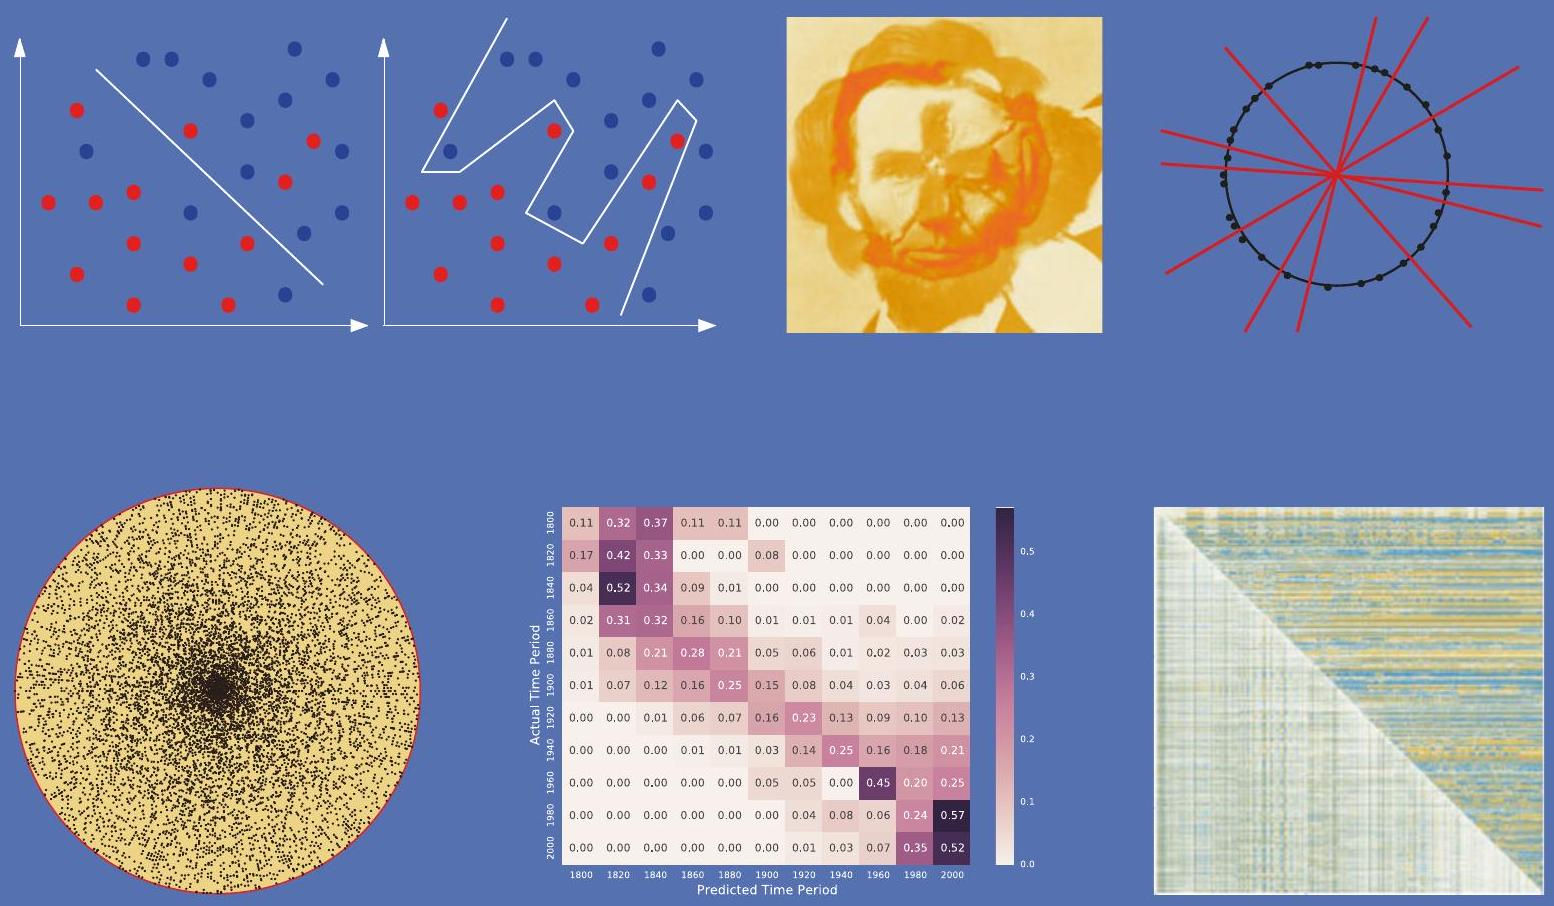
\includegraphics[max width=\textwidth]{2025_03_17_ca60ec0bfd96dcf8e028g-001}
\end{center}

\section*{Steven S. Skiena}
Springer
\begin{itemize}
\item ISBN 978-3-319-55443-3
\item ISBN 978-3-319-55444-0 (eBook)
\item \href{https://doi.org/10.1007/978-3-319-55444-0}{https://doi.org/10.1007/978-3-319-55444-0}
\end{itemize}

\section*{Preface}
Making sense of the world around us requires obtaining and analyzing data from our environment. Several technology trends have recently collided, providing new opportunities to apply our data analysis savvy to greater challenges than ever before.

Computer storage capacity has increased exponentially; indeed remembering has become so cheap that it is almost impossible to get computer systems to forget. Sensing devices increasingly monitor everything that can be observed: video streams, social media interactions, and the position of anything that moves. Cloud computing enables us to harness the power of massive numbers of machines to manipulate this data. Indeed, hundreds of computers are summoned each time you do a Google search, scrutinizing all of your previous activity just to decide which is the best ad to show you next.

The result of all this has been the birth of \textit{data science}, a new field devoted to maximizing value from vast collections of information. As a discipline, data science sits somewhere at the intersection of statistics, computer science, and machine learning, but it is building a distinct heft and character of its own. This book serves as an introduction to data science, focusing on the skills and principles needed to build systems for collecting, analyzing, and interpreting data.

My professional experience as a researcher and instructor convinces me that one major challenge of data science is that it is considerably more subtle than it looks. Any student who has ever computed their grade point average (GPA) can be said to have done rudimentary statistics, just as drawing a simple scatter plot lets you add experience in data visualization to your resume. But meaningfully analyzing and interpreting data requires both technical expertise and wisdom. That so many people do these basics so badly provides my inspiration for writing this book.

\section*{To the Reader}
I have been gratified by the warm reception that my book \textit{The Algorithm Design Manual} [\cite{skiena2008algorithm}] has received since its initial publication in 1997. It has been recognized as a unique guide to using algorithmic techniques to solve problems that often arise in practice. The book you are holding covers very different material, but with the same motivation.

In particular, here I stress the following basic principles as fundamental to becoming a good data scientist:

\begin{itemize}
  \item \textit{Valuing doing the simple things right}: Data science isn't rocket science. Students and practitioners often get lost in technological space, pursuing the most advanced machine learning methods, the newest open source software libraries, or the glitziest visualization techniques. However, the heart of data science lies in doing the simple things right: understanding the application domain, cleaning and integrating relevant data sources, and presenting your results clearly to others.

Simple doesn't mean easy, however. Indeed it takes considerable insight and experience to ask the right questions, and sense whether you are moving toward correct answers and actionable insights. I resist the temptation to drill deeply into clean, technical material here just because it is teachable. There are plenty of other books which will cover the intricacies of machine learning algorithms or statistical hypothesis testing. My mission here is to lay the groundwork of what really matters in analyzing data.

  \item \textit{Developing mathematical intuition}: Data science rests on a foundation of mathematics, particularly statistics and linear algebra. It is important to understand this material on an intuitive level: why these concepts were developed, how they are useful, and when they work best. I illustrate operations in linear algebra by presenting pictures of what happens to matrices when you manipulate them, and statistical concepts by examples and reducto ad absurdum arguments. My goal here is transplanting intuition into the reader.

But I strive to minimize the amount of formal mathematics used in presenting this material. Indeed, I will present exactly one formal proof in this book, an incorrect proof where the associated theorem is obviously false. The moral here is not that mathematical rigor doesn't matter, because of course it does, but that genuine rigor is impossible until after there is comprehension.

  \item \textit{Think like a computer scientist, but act like a statistician}: Data science provides an umbrella linking computer scientists, statisticians, and domain specialists. But each community has its own distinct styles of thinking and action, which gets stamped into the souls of its members.

In this book, I emphasize approaches which come most naturally to computer scientists, particularly the algorithmic manipulation of data, the use of machine learning, and the mastery of scale. But I also seek to transmit the core values of statistical reasoning: the need to understand the application domain, proper appreciation of the small, the quest for significance, and a hunger for exploration.

No discipline has a monopoly on the truth. The best data scientists incorporate tools from multiple areas, and this book strives to be a relatively neutral ground where rival philosophies can come to reason together.
\end{itemize}

Equally important is what you will not find in this book. I do not emphasize any particular language or suite of data analysis tools. Instead, this book provides a high-level discussion of important design principles. I seek to operate at a conceptual level more than a technical one. The goal of this manual is to get you going in the right direction as quickly as possible, with whatever software tools you find most accessible.

\section*{To the Instructor}
This book covers enough material for an \textit{Introduction to Data Science} course at the undergraduate or early graduate student levels. I hope that the reader has completed the equivalent of at least one programming course and has a bit of prior exposure to probability and statistics, but more is always better than less.

I have made a full set of lecture slides for teaching this course available online at \href{http://www.data-manual.com}{http://www.data-manual.com}. Data resources for projects and assignments are also available there to aid the instructor. Further, I make available online video lectures using these slides to teach a full-semester data science course. Let me help teach your class, through the magic of the web!

Pedagogical features of this book include:

\begin{itemize}
  \item \textit{War Stories}: To provide a better perspective on how data science techniques apply to the real world, I include a collection of "war stories," or tales from our experience with real problems. The moral of these stories is that these methods are not just theory, but important tools to be pulled out and used as needed.
  \item \textit{False Starts}: Most textbooks present methods as a fait accompli, obscuring the ideas involved in designing them, and the subtle reasons why other approaches fail. The war stories illustrate my reasoning process on certain applied problems, but I weave such coverage into the core material as well.
  \item \textit{Take-Home Lessons}: Highlighted "take-home" lesson boxes scattered through each chapter emphasize the big-picture concepts to learn from each chapter.
  \item \textit{Homework Problems}: I provide a wide range of exercises for homework and self-study. Many are traditional exam-style problems, but there are also larger-scale implementation challenges and smaller-scale interview questions, reflecting the questions students might encounter when searching for a job. Degree of difficulty ratings have been assigned to all problems.
In lieu of an answer key, a Solution Wiki has been set up, where solutions to all even numbered problems will be solicited by crowdsourcing. A similar system with my \textit{Algorithm Design Manual} produced coherent solutions, or so I am told. As a matter of principle I refuse to look at them, so let the buyer beware.
  \item \textit{Kaggle Challenges}: Kaggle (\href{http://www.kaggle.com}{www.kaggle.com}) provides a forum for data scientists to compete in, featuring challenging real-world problems on fascinating data sets, and scoring to test how good your model is relative to other submissions. The exercises for each chapter include three relevant Kaggle challenges, to serve as a source of inspiration, self-study, and data for other projects and investigations.
  \item \textit{Data Science Television}: Data science remains mysterious and even threatening to the broader public. \textit{The Quant Shop} is an amateur take on what a data science reality show should be like. Student teams tackle a diverse array of real-world prediction problems, and try to forecast the outcome of future events. Check it out at \href{http://www.quant-shop.com}{http://www.quant-shop.com}.

A series of eight 30-minute episodes has been prepared, each built around a particular real-world prediction problem. Challenges include pricing art at an auction, picking the winner of the Miss Universe competition, and forecasting when celebrities are destined to die. For each, we observe as a student team comes to grips with the problem, and learn along with them as they build a forecasting model. They make their predictions, and we watch along with them to see if they are right or wrong.

In this book, \textit{The Quant Shop} is used to provide concrete examples of prediction challenges, to frame discussions of the data science modeling pipeline from data acquisition to evaluation. I hope you find them fun, and that they will encourage you to conceive and take on your own modeling challenges.
  \item \textit{Chapter Notes}: Finally, each tutorial chapter concludes with a brief notes section, pointing readers to primary sources and additional references.
\end{itemize}

\section*{Dedication}
My bright and loving daughters Bonnie and Abby are now full-blown teenagers, meaning that they don't always process statistical evidence with as much alacrity as I would I desire. I dedicate this book to them, in the hope that their analysis skills improve to the point that they always just agree with me.

And I dedicate this book to my beautiful wife Renee, who agrees with me even when she doesn't agree with me, and loves me beyond the support of all creditable evidence.

\section*{Acknowledgments}
My list of people to thank is large enough that I have probably missed some. I will try to do enumerate them systematically to minimize omissions, but ask those I've unfairly neglected for absolution.

First, I thank those who made concrete contributions to help me put this book together. Yeseul Lee served as an apprentice on this project, helping with figures, exercises, and more during summer 2016 and beyond. You will see evidence of her handiwork on almost every page, and I greatly appreciate her help and dedication. Aakriti Mittal and Jack Zheng also contributed to a few of the figures.

Students in my Fall 2016 \textit{Introduction to Data Science} course (CSE 519) helped to debug the manuscript, and they found plenty of things to debug. I particularly thank Rebecca Siford, who proposed over one hundred corrections on her own. Several data science friends/sages reviewed specific chapters for me, and I thank Anshul Gandhi, Yifan Hu, Klaus Mueller, Francesco Orabona, Andy Schwartz, and Charles Ward for their efforts here.

I thank all the \textit{Quant Shop} students from Fall 2015 whose video and modeling efforts are so visibly on display. I particularly thank Jan (Dini) DiskinZimmerman, whose editing efforts went so far beyond the call of duty I felt like a felon for letting her do it.

My editors at Springer, Wayne Wheeler and Simon Rees, were a pleasure to work with as usual. I also thank all the production and marketing people who helped get this book to you, including Adrian Pieron and Annette Anlauf.

Several exercises were originated by colleagues or inspired by other sources. Reconstructing the original sources years later can be challenging, but credits for each problem (to the best of my recollection) appear on the website.

Much of what I know about data science has been learned through working with other people. These include my Ph.D. students, particularly Rami al-Rfou, Mikhail Bautin, Haochen Chen, Yanqing Chen, Vivek Kulkarni, Levon Lloyd, Andrew Mehler, Bryan Perozzi, Yingtao Tian, Junting Ye, Wenbin Zhang, and postdoc Charles Ward. I fondly remember all of my Lydia project masters students over the years, and remind you that my prize offer to the first one who names their daughter Lydia remains unclaimed. I thank my other collaborators with stories to tell, including Bruce Futcher, Justin Gardin, Arnout van de Rijt, and Oleksii Starov.

I remember all members of the General Sentiment/Canrock universe, particularly Mark Fasciano, with whom I shared the start-up dream and experienced what happens when data hits the real world. I thank my colleagues at Yahoo Labs/Research during my 2015-2016 sabbatical year, when much of this book was conceived. I single out Amanda Stent, who enabled me to be at Yahoo during that particularly difficult year in the company's history. I learned valuable things from other people who have taught related data science courses, including Andrew Ng and Hans-Peter Pfister, and thank them all for their help.

If you have a procedure with ten parameters, you probably missed some.

\section*{Caveat}
It is traditional for the author to magnanimously accept the blame for whatever deficiencies remain. I don't. Any errors, deficiencies, or problems in this book are somebody else's fault, but I would appreciate knowing about them so as to determine who is to blame.

\section*{Contents}
\begin{itemize}
  \item What is Data Science?
  \begin{itemize}
    \item Computer Science, Data Science, and Real Science
    \item Asking Interesting Questions from Data
    \begin{itemize}
      \item The Baseball Encyclopedia
      \item The Internet Movie Database (IMDb)
      \item Google Ngrams
      \item New York Taxi Records
    \end{itemize}
  \end{itemize}
  \item Mathematical Preliminaries
  \begin{itemize}
    \item Probability
    \begin{itemize}
      \item Probability vs. Statistics
      \item Compound Events and Independence
      \item Conditional Probability
      \item Probability Distributions
    \end{itemize}
  \end{itemize}
\end{itemize}

\section*{Chapter 1}
\section*{What is Data Science?}
\textit{The purpose of computing is insight, not numbers.} -- Richard W. Hamming

What is data science? Like any emerging field, it hasn't been completely defined yet, but you know enough about it to be interested or else you wouldn't be reading this book.

I think of data science as lying at the intersection of computer science, statistics, and substantive application domains. From computer science comes machine learning and high-performance computing technologies for dealing with scale. From statistics comes a long tradition of exploratory data analysis, significance testing, and visualization. From application domains in business and the sciences comes challenges worthy of battle, and evaluation standards to assess when they have been adequately conquered.

But these are all well-established fields. Why data science, and why now? I see three reasons for this sudden burst of activity:

\begin{itemize}
  \item \textit{New technology makes it possible to capture, annotate, and store vast amounts of social media, logging, and sensor data.} After you have amassed all this data, you begin to wonder what you can do with it.
  \item \textit{Computing advances make it possible to analyze data in novel ways and at ever increasing scales.} Cloud computing architectures give even the little guy access to vast power when they need it. New approaches to machine learning have lead to amazing advances in longstanding problems, like computer vision and natural language processing.
  \item \textit{Prominent technology companies (like Google and Facebook) and quantitative hedge funds (like Renaissance Technologies and TwoSigma) have proven the power of modern data analytics.} Success stories applying data to such diverse areas as sports management (\textit{Moneyball} [\cite{lewis2004moneyball}]) and election forecasting (Nate Silver [\cite{silver2012signal}]) have served as role models to bring data science to a large popular audience.
\end{itemize}

This introductory chapter has three missions. First, I will try to explain how good data scientists think, and how this differs from the mindset of traditional programmers and software developers. Second, we will look at data sets in terms of the potential for what they can be used for, and learn to ask the broader questions they are capable of answering. Finally, I introduce a collection of data analysis challenges that will be used throughout this book as motivating examples.

\subsection*{Computer Science, Data Science, and Real Science}
Computer scientists, by nature, don't respect data. They have traditionally been taught that the algorithm was the thing, and that data was just meat to be passed through a sausage grinder.

So to qualify as an effective data scientist, you must first learn to think like a real scientist. Real scientists strive to understand the natural world, which is a complicated and messy place. By contrast, computer scientists tend to build their own clean and organized virtual worlds and live comfortably within them. Scientists obsess about discovering things, while computer scientists invent rather than discover.

People's mindsets strongly color how they think and act, causing misunderstandings when we try to communicate outside our tribes. So fundamental are these biases that we are often unaware we have them. Examples of the cultural differences between computer science and real science include:

\begin{itemize}
  \item \textit{Data vs. method centrism}: Scientists are data driven, while computer scientists are algorithm driven. Real scientists spend enormous amounts of effort collecting data to answer their question of interest. They invent fancy measuring devices, stay up all night tending to experiments, and devote most of their thinking to how to get the data they need.

By contrast, computer scientists obsess about methods: which algorithm is better than which other algorithm, which programming language is best for a job, which program is better than which other program. The details of the data set they are working on seem comparably unexciting.

  \item \textit{Concern about results}: Real scientists care about answers. They analyze data to discover something about how the world works. Good scientists care about whether the results make sense, because they care about what the answers mean.

By contrast, bad computer scientists worry about producing plausible-looking numbers. As soon as the numbers stop looking grossly wrong, they are presumed to be right. This is because they are personally less invested in what can be learned from a computation, as opposed to getting it done quickly and efficiently.

  \item \textit{Robustness}: Real scientists are comfortable with the idea that data has errors. In general, computer scientists are not. Scientists think a lot about possible sources of bias or error in their data, and how these possible problems can effect the conclusions derived from them. Good programmers use strong data-typing and parsing methodologies to guard against formatting errors, but the concerns here are different.

Becoming aware that data can have errors is empowering. Computer scientists chant "garbage in, garbage out" as a defensive mantra to ward off criticism, a way to say \textit{that's not my job}. Real scientists get close enough to their data to smell it, giving it the sniff test to decide whether it is likely to be garbage.

  \item \textit{Precision}: Nothing is ever completely true or false in science, while \textit{everything} is either true or false in computer science or mathematics.

Generally speaking, computer scientists are happy printing floating point numbers to as many digits as possible: \(8/13=0.61538461538\). Real scientists will use only two significant digits: \(8/13 \approx 0.62\). Computer scientists care what a number is, while real scientists care what it means.
\end{itemize}

Aspiring data scientists must learn to think like real scientists. Your job is going to be to turn numbers into insight. It is important to understand the \textit{why} as much as the \textit{how}.

To be fair, it benefits real scientists to think like data scientists as well. New experimental technologies enable measuring systems on vastly greater scale than ever possible before, through technologies like full-genome sequencing in biology and full-sky telescope surveys in astronomy. With new breadth of view comes new levels of vision.

Traditional \textit{hypothesis-driven} science was based on asking specific questions of the world and then generating the specific data needed to confirm or deny it. This is now augmented by \textit{data-driven} science, which instead focuses on generating data on a previously unheard of scale or resolution, in the belief that new discoveries will come as soon as one is able to look at it. Both ways of thinking will be important to us:

\begin{itemize}
  \item Given a problem, what available data will help us answer it?
  \item Given a data set, what interesting problems can we apply it to?
\end{itemize}

There is another way to capture this basic distinction between software engineering and data science. It is that software developers are hired to build systems, while data scientists are hired to produce insights.

This may be a point of contention for some developers. There exist an important class of engineers who wrangle the massive distributed infrastructures necessary to store and analyze, say, financial transaction or social media data on a full Facebook or Twitter-level of scale. Indeed, I will devote Chapter 12 to the distinctive challenges of big data infrastructures. These engineers are building tools and systems to support data science, even though they may not personally mine the data they wrangle. Do they qualify as data scientists?

This is a fair question, one I will finesse a bit so as to maximize the potential readership of this book. But I do believe that the better such engineers understand the full data analysis pipeline, the more likely they will be able to build powerful tools capable of providing important insights. A major goal of this book is providing big data engineers with the intellectual tools to think like big data scientists.

\subsection*{Asking Interesting Questions from Data}
Good data scientists develop an inherent curiosity about the world around them, particularly in the associated domains and applications they are working on. They enjoy talking shop with the people whose data they work with. They ask them questions: What is the coolest thing you have learned about this field? Why did you get interested in it? What do you hope to learn by analyzing your data set? Data scientists always ask questions.

Good data scientists have wide-ranging interests. They read the newspaper every day to get a broader perspective on what is exciting. They understand that the world is an interesting place. Knowing a little something about everything equips them to play in other people's backyards. They are brave enough to get out of their comfort zones a bit, and driven to learn more once they get there.

Software developers are not really encouraged to ask questions, but data scientists are. We ask questions like:

\begin{itemize}
  \item What things might you be able to learn from a given data set?
  \item What do you/your people really want to know about the world?
  \item What will it mean to you once you find out?
\end{itemize}

Computer scientists traditionally do not really appreciate data. Think about the way algorithm performance is experimentally measured. Usually the program is run on "random data" to see how long it takes. They rarely even look at the results of the computation, except to verify that it is correct and efficient. Since the "data" is meaningless, the results cannot be important. In contrast, real data sets are a scarce resource, which required hard work and imagination to obtain.

Becoming a data scientist requires learning to ask questions about data, so let's practice. Each of the subsections below will introduce an interesting data set. After you understand what kind of information is available, try to come up with, say, five interesting questions you might explore/answer with access to this data set.

\begin{figure}[h]
    \centering
    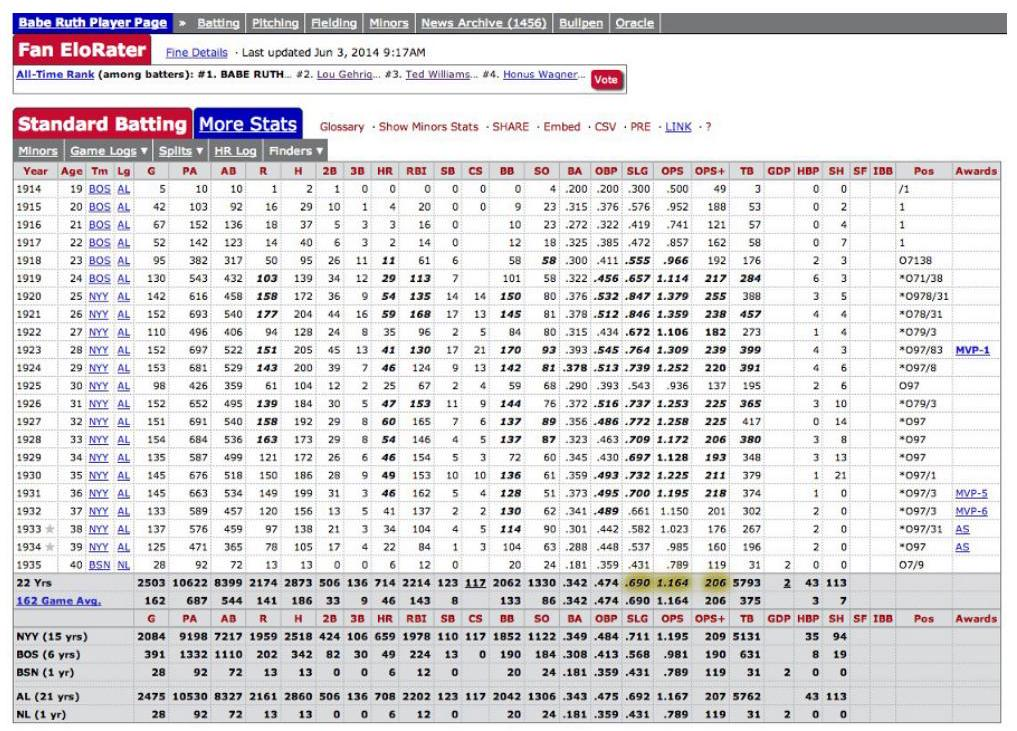
\includegraphics[max width=\textwidth, center]{2025_03_17_ca60ec0bfd96dcf8e028g-023}
    \caption{Statistical information on the performance of Babe Ruth can be found at \href{http://www.baseball-reference.com}{http://www.baseball-reference.com}.}
\end{figure}

The key is thinking broadly: the answers to big, general questions often lie buried in highly-specific data sets, which were by no means designed to contain them.

\subsubsection*{The Baseball Encyclopedia}
Baseball has long had an outsized importance in the world of data science. This sport has been called the national pastime of the United States; indeed, French historian Jacques Barzun observed that "Whoever wants to know the heart and mind of America had better learn baseball." I realize that many readers are not American, and even those that are might be completely disinterested in sports. But stick with me for a while.

What makes baseball important to data science is its extensive statistical record of play, dating back for well over a hundred years. Baseball is a sport of discrete events: pitchers throw balls and batters try to hit them - that naturally lends itself to informative statistics. Fans get immersed in these statistics as children, building their intuition about the strengths and limitations of quantitative analysis. Some of these children grow up to become data scientists. Indeed, the success of Brad Pitt's statistically-minded baseball team in the movie \textit{Moneyball} remains the American public's most vivid contact with data science.

This historical baseball record is available at \href{http://www.baseball-reference.com}{http://www.baseball-reference.com}. There you will find complete statistical data on the performance of every player who even stepped on the field. This includes summary statistics of each season's batting, pitching, and fielding record, plus information about teams

\begin{figure}[h]
    \centering
    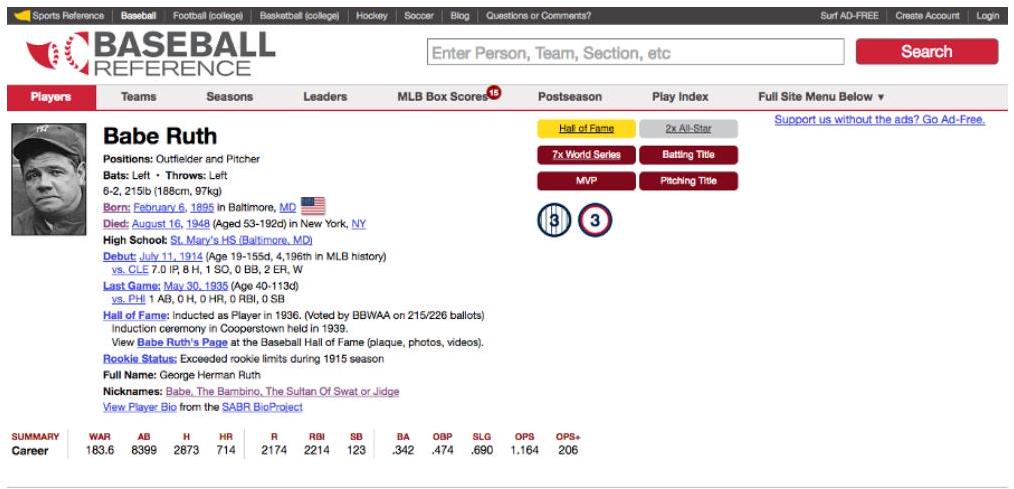
\includegraphics[max width=\textwidth, center]{2025_03_17_ca60ec0bfd96dcf8e028g-024}
    \caption{Personal information on every major league baseball player is available at \href{http://www.baseball-reference.com}{http://www.baseball-reference.com}.}
\end{figure}

and awards as shown in Figure 1.1.

But more than just statistics, there is metadata on the life and careers of all the people who have ever played major league baseball, as shown in Figure 1.2. We get the vital statistics of each player (height, weight, handedness) and their lifespan (when/where they were born and died). We also get salary information (how much each player got paid every season) and transaction data (how did they get to be the property of each team they played for).

Now, I realize that many of you do not have the slightest knowledge of or interest in baseball. This sport is somewhat reminiscent of cricket, if that helps. But remember that as a data scientist, it is your job to be interested in the world around you. Think of this as a chance to learn something.

So what interesting questions can you answer with this baseball data set? Try to write down five questions before moving on. Don't worry, I will wait here for you to finish.

The most obvious types of questions to answer with this data are directly related to baseball:

\begin{itemize}
  \item How can we best measure an individual player's skill or value?
  \item How fairly do trades between teams generally work out?
  \item What is the general trajectory of player's performance level as they mature and age?
  \item To what extent does batting performance correlate with position played? For example, are outfielders really better hitters than infielders?
\end{itemize}

These are interesting questions. But even more interesting are questions about demographic and social issues. Almost 20,000 major league baseball players have taken the field over the past 150 years, providing a large, extensively-documented cohort of men who can serve as a proxy for even larger, less well-documented populations. Indeed, we can use this baseball player data to answer questions like:

\begin{itemize}
  \item Do left-handed people have shorter lifespans than right-handers? Handedness is not captured in most demographic data sets, but has been diligently assembled here. Indeed, analysis of this data set has been used to show that right-handed people live longer than lefties [\cite{halpern1988right}]!
  \item How often do people return to live in the same place where they were born? Locations of birth and death have been extensively recorded in this data set. Further, almost all of these people played at least part of their career far from home, thus exposing them to the wider world at a critical time in their youth.
  \item Do player salaries generally reflect past, present, or future performance?
  \item To what extent have heights and weights been increasing in the population at large?
\end{itemize}

There are two particular themes to be aware of here. First, the identifiers and reference tags (i.e. the metadata) often prove more interesting in a data set than the stuff we are supposed to care about, here the statistical record of play.

Second is the idea of a \textit{statistical proxy}, where you use the data set you have to substitute for the one you really want. The data set of your dreams likely does not exist, or may be locked away behind a corporate wall even if it does. A good data scientist is a pragmatist, seeing what they can do with what they have instead of bemoaning what they cannot get their hands on.

\subsubsection*{The Internet Movie Database (IMDb)}
Everybody loves the movies. The Internet Movie Database (IMDb) provides crowdsourced and curated data about all aspects of the motion picture industry, at \href{http://www.imdb.com}{www.imdb.com}. IMDb currently contains data on over 3.3 million movies and TV programs. For each film, IMDb includes its title, running time, genres, date of release, and a full list of cast and crew. There is financial data about each production, including the budget for making the film and how well it did at the box office.

Finally, there are extensive ratings for each film from viewers and critics. This rating data consists of scores on a zero to ten stars scale, cross-tabulated into averages by age and gender. Written reviews are often included, explaining why a particular critic awarded a given number of stars. There are also links between films: for example, identifying which other films have been watched most often by viewers of \textit{It's a Wonderful Life}.

Every actor, director, producer, and crew member associated with a film merits an entry in IMDb, which now contains records on 6.5 million people.

\begin{figure}[h]
    \centering
    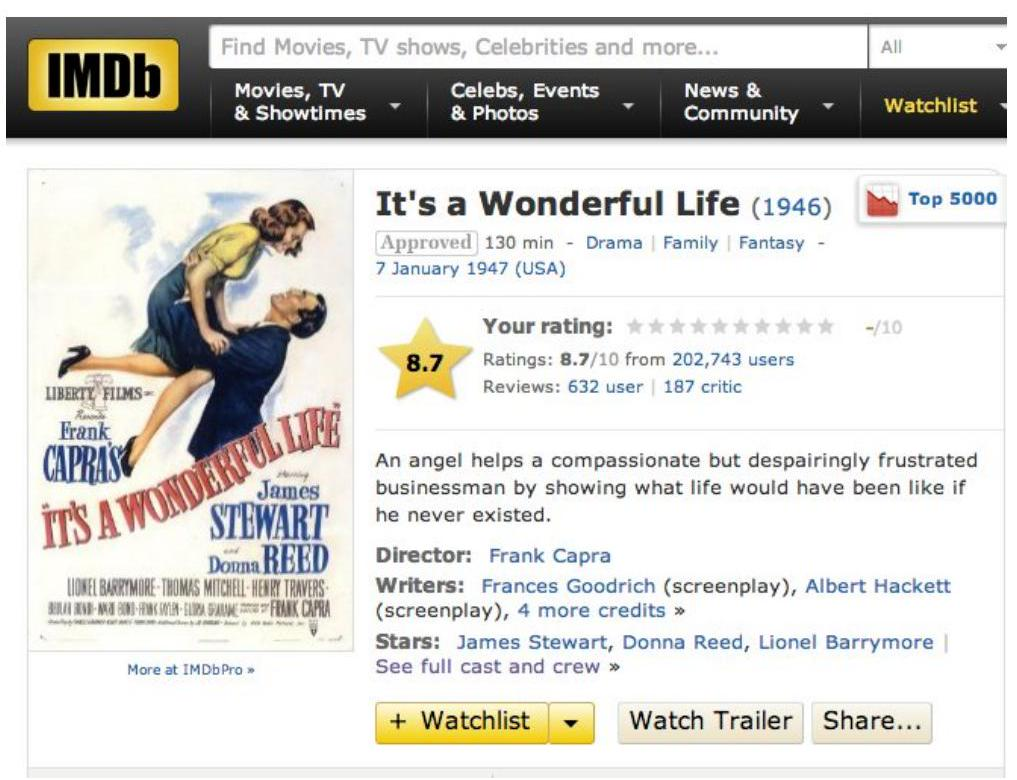
\includegraphics[max width=\textwidth, center]{2025_03_17_ca60ec0bfd96dcf8e028g-026}
    \caption{Representative film data from the Internet Movie Database.}
\end{figure}

\begin{figure}[h]
    \centering
    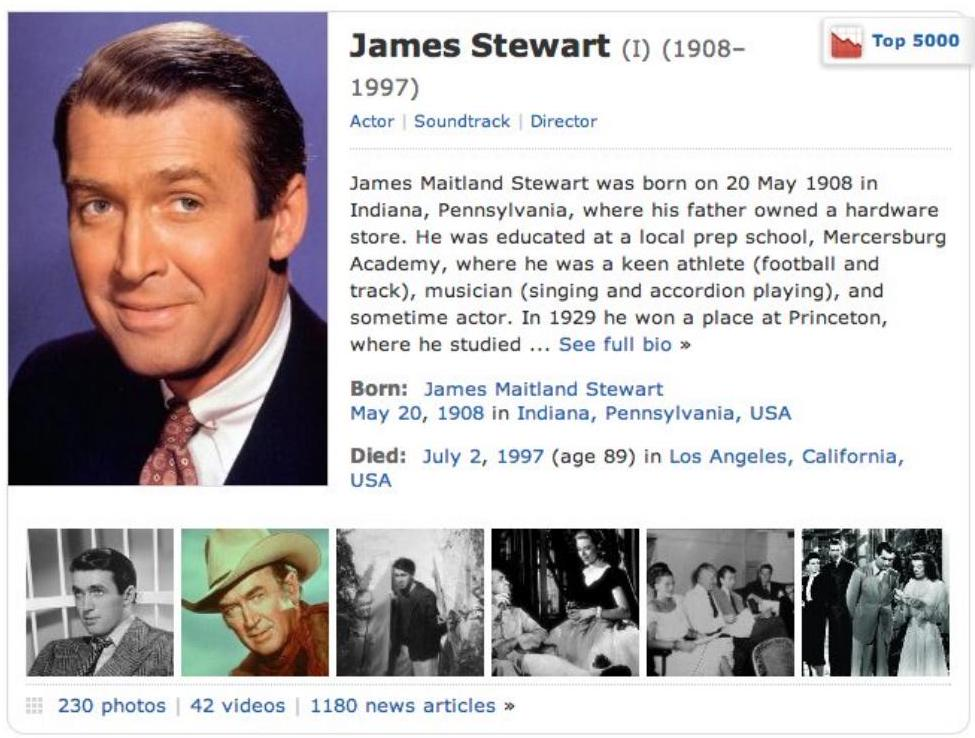
\includegraphics[max width=\textwidth, center]{2025_03_17_ca60ec0bfd96dcf8e028g-026(1)}
    \caption{Representative actor data from the Internet Movie Database.}
\end{figure}

These happen to include my brother, cousin, and sister-in-law. Each actor is linked to every film they appeared in, with a description of their role and their ordering in the credits. Available data about each personality includes birth/death dates, height, awards, and family relations.

So what kind of questions can you answer with this movie data?

Perhaps the most natural questions to ask IMDb involve identifying the extremes of movies and actors:

\begin{itemize}
  \item Which actors appeared in the most films? Earned the most money? Appeared in the lowest rated films? Had the longest career or the shortest lifespan?
  \item What was the highest rated film each year, or the best in each genre? Which movies lost the most money, had the highest-powered casts, or got the least favorable reviews.
\end{itemize}

Then there are larger-scale questions one can ask about the nature of the motion picture business itself:

\begin{itemize}
  \item How well does movie gross correlate with viewer ratings or awards? Do customers instinctively flock to trash, or is virtue on the part of the creative team properly rewarded?
  \item How do Hollywood movies compare to Bollywood movies, in terms of ratings, budget, and gross? Are American movies better received than foreign films, and how does this differ between U.S. and non-U.S. reviewers?
  \item What is the age distribution of actors and actresses in films? How much younger is the actress playing the wife, on average, than the actor playing the husband? Has this disparity been increasing or decreasing with time?
  \item Live fast, die young, and leave a good-looking corpse? Do movie stars live longer or shorter lives than bit players, or compared to the general public?
\end{itemize}

Assuming that people working together on a film get to know each other, the cast and crew data can be used to build a social network of the movie business. What does the social network of actors look like? The Oracle of Bacon (\href{https://oracleofbacon.org/}{https://oracleofbacon.org/}) posits Kevin Bacon as the center of the Hollywood universe and generates the shortest path to Bacon from any other actor. Other actors, like Samuel L. Jackson, prove even more central.

More critically, can we analyze this data to determine the probability that someone will like a given movie? The technique of \textit{collaborative filtering} finds people who liked films that I also liked, and recommends other films that they liked as good candidates for me. The 2007 Netflix Prize was a \$1,000,000 competition to produce a ratings engine 10\% better than the proprietary Netflix system. The ultimate winner of this prize (BellKor) used a variety of data sources and techniques, including the analysis of links [\cite{bell2007lessons}].

\begin{figure}[h]
    \centering
    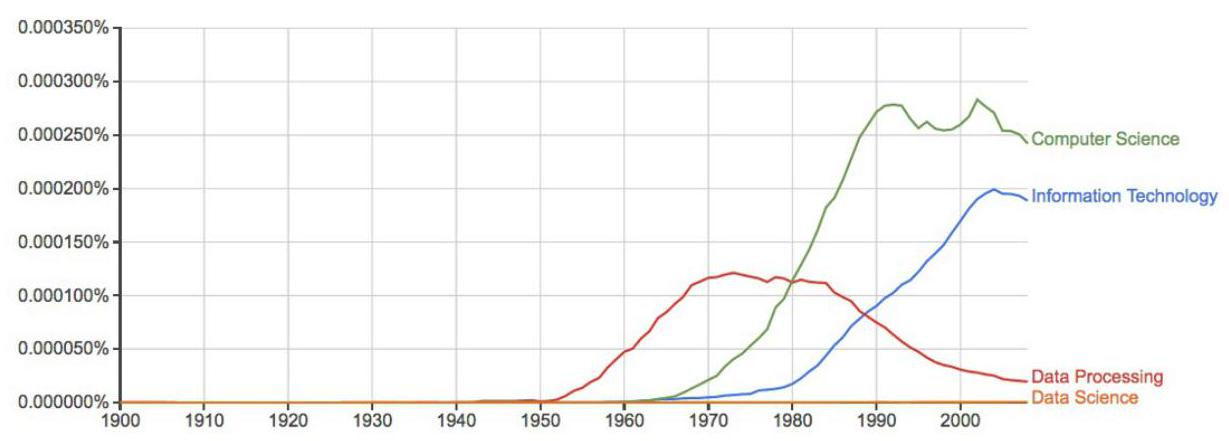
\includegraphics[max width=\textwidth, center]{2025_03_17_ca60ec0bfd96dcf8e028g-028}
    \caption{The rise and fall of data processing, as witnessed by Google Ngrams.}
\end{figure}

\subsubsection*{Google Ngrams}
Printed books have been the primary repository of human knowledge since Gutenberg's invention of movable type in 1439. Physical objects live somewhat uneasily in today's digital world, but technology has a way of reducing everything to data. As part of its mission to organize the world's information, Google undertook an effort to scan all of the world's published books. They haven't quite gotten there yet, but the 30 million books thus far digitized represent over 20\% of all books ever published.

Google uses this data to improve search results, and provide fresh access to out-of-print books. But perhaps the coolest product is \textit{Google Ngrams}, an amazing resource for monitoring changes in the cultural zeitgeist. It provides the frequency with which short phrases occur in books published each year. Each phrase must occur at least forty times in their scanned book corpus. This eliminates obscure words and phrases, but leaves over two billion time series available for analysis.

This rich data set shows how language use has changed over the past 200 years, and has been widely applied to cultural trend analysis [MAV$^{+}$11]. Figure 1.5 uses this data to show how the word \textit{data} fell out of favor when thinking about computing. \textit{Data processing} was the popular term associated with the computing field during the punched card and spinning magnetic tape era of the 1950s. The Ngrams data shows that the rapid rise of \textit{Computer Science} did not eclipse \textit{Data Processing} until 1980. Even today, \textit{Data Science} remains almost invisible on this scale.

Check out Google Ngrams at \href{http://books.google.com/ngrams}{http://books.google.com/ngrams}. I promise you will enjoy playing with it. Compare \textit{hot dog} to \textit{tofu}, \textit{science} against \textit{religion}, \textit{freedom} to \textit{justice}, and \textit{sex} vs. \textit{marriage}, to better understand this fantastic telescope for looking into the past.

But once you are done playing, think of bigger things you could do if you got your hands on this data. Assume you have access to the annual number of references for \textit{all} words/phrases published in books over the past 200 years.

Google makes this data freely available. So what are you going to do with it?

Observing the time series associated with particular words using the Ngrams Viewer is fun. But more sophisticated historical trends can be captured by aggregating multiple time series together. The following types of questions seem particularly interesting to me:

\begin{itemize}
  \item How has the amount of cursing changed over time? Use of the four-letter words I am most familiar with seem to have exploded since 1960, although it is perhaps less clear whether this reflects increased cussing or lower publication standards.
  \item How often do new words emerge and get popular? Do these words tend to stay in common usage, or rapidly fade away? Can we detect when words change meaning over time, like the transition of \textit{gay} from \textit{happy} to \textit{homosexual}?
  \item Have standards of spelling been improving or deteriorating with time, especially now that we have entered the era of automated spell checking? Rarely-occurring words that are only one character removed from a commonly-used word are likely candidates to be spelling errors (e.g. \textit{algorithm} vs. \textit{algorthm}). Aggregated over many different misspellings, are such errors increasing or decreasing?
\end{itemize}

You can also use this Ngrams corpus to build a language model that captures the meaning and usage of the words in a given language. We will discuss word embeddings in Section 11.6.3, which are powerful tools for building language models. Frequency counts reveal which words are most popular. The frequency of word pairs appearing next to each other can be used to improve speech recognition systems, helping to distinguish whether the speaker said \textit{that's too bad} or \textit{that's to bad}. These millions of books provide an ample data set to build representative models from.

\subsubsection*{New York Taxi Records}
Every financial transaction today leaves a data trail behind it. Following these paths can lead to interesting insights.

Taxi cabs form an important part of the urban transportation network. They roam the streets of the city looking for customers, and then drive them to their destination for a fare proportional to the length of the trip. Each cab contains a metering device to calculate the cost of the trip as a function of time. This meter serves as a record keeping device, and a mechanism to ensure that the driver charges the proper amount for each trip.

The taxi meters currently employed in New York cabs can do many things beyond calculating fares. They act as credit card terminals, providing a way

\begin{table}[h]
\centering
\begin{tabular}{|c|c|c|c|c|c|c|c|c|c|}
\hline
Vendor ID & Passenger Count & Trip Distance & Pickup Longitude & Pickup Latitude & Dropoff Longitude & Dropoff Latitude & Payment Type & Tip Amount & Total Amount \\
\hline
2 & 1 & 7.22 & -73.9998 & 40.74334 & -73.9428 & 40.80662 & 2 & 0 & 30.8 \\
1 & 1 & 2.3 & -73.977 & 40.7749 & -73.9783 & 40.74986 & 1 & 2.93 & 16.23 \\
1 & 1 & 1.5 & -73.9591 & 40.77513 & -73.9804 & 40.78231 & 1 & 1.65 & 9.95 \\
1 & 1 & 0.9 & -73.9766 & 40.78075 & -73.9706 & 40.78885 & 1 & 1.45 & 8.75 \\
2 & 1 & 2.44 & -73.9786 & 40.78592 & -73.9974 & 40.7563 & 1 & 2 & 16.3 \\
2 & 1 & 3.36 & -73.9764 & 40.78589 & -73.9424 & 40.82209 & 1 & 3.58 & 17.88 \\
2 & 2 & 2.34 & -73.9862 & 40.76087 & -73.9569 & 40.77156 & 1 & 1 & 13.8 \\
2 & 1 & 10.19 & -73.79 & 40.64406 & -73.9312 & 40.67588 & 2 & 0 & 32.8 \\
1 & 2 & 3.3 & -73.9937 & 40.72738 & -73.9982 & 40.7641 & 1 & 2 & 21.3 \\
1 & 1 & 1.8 & -73.9949 & 40.74006 & -73.9767 & 40.74934 & 1 & 1.85 & 11.15 \\
\hline
\end{tabular}
\caption{Representative fields from the New York city taxi cab data: pick-up and drop-off points, distances, and fares.}
\end{table}

for customers to pay for rides without cash. They are integrated with Global Positioning Systems (GPS), recording the exact location of every pickup and drop off. And finally, since they are on a wireless network, these boxes can communicate all of this data back to a central server.

The result is a database documenting every single trip by all taxi cabs in one of the world's greatest cities, a small portion of which is shown in Table 1. The New York Taxi and Limousine Commission is a public agency, its non-confidential data is available to all under the Freedom of Information Act (FOA).

Every ride generates two records: one with data on the trip, the other with details of the fare. Each trip is keyed to the medallion (license) of each car coupled with the identifier of each driver. For each trip, we get the time/date of pickup and drop-off, as well as the GPS coordinates (longitude and latitude) of the starting location and destination. We do not get GPS data of the route they traveled between these points, but to some extent that can be inferred by the shortest path between them.

As for fare data, we get the metered cost of each trip, including tax, surcharge and tolls. It is traditional to pay the driver a tip for service, the amount of which is also recorded in the data.

So I'm talking to you. This taxi data is readily available, with records of over 80 million trips over the past several years. What are you going to do with it?

Any interesting data set can be used to answer questions on many different scales. This taxi fare data can help us better understand the transportation industry, but also how the city works and how we could make it work even better. Natural questions with respect to the taxi industry include:
```
%---- Page End Break Here ---- Page : 12
```latex
\begin{figure}[h!]
\centering
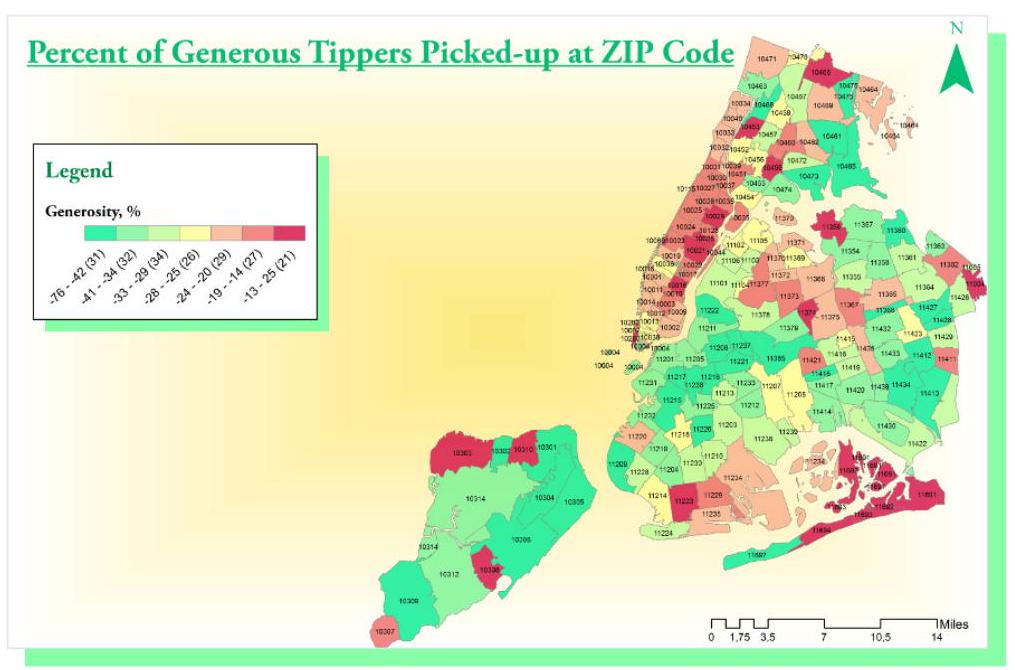
\includegraphics[max width=\textwidth]{2025_03_17_ca60ec0bfd96dcf8e028g-031}
\caption{Which neighborhoods in New York City tip most generously? The relatively remote outer boroughs of Brooklyn and Queens, where trips are longest and supply is relatively scarce.}
\label{fig:1.7}
\end{figure}

\begin{itemize}
  \item How much money do drivers make each night, on average? What is the distribution? Do drivers make more on sunny days or rainy days?
  \item Where are the best spots in the city for drivers to cruise, in order to pick up profitable fares? How does this vary at different times of the day?
  \item How far do drivers travel over the course of a night's work? We can't answer this exactly using this data set, because it does not provide GPS data of the route traveled between fares. But we do know the last place of drop off, the next place of pickup, and how long it took to get between them. Together, this should provide enough information to make a sound estimate.
  \item Which drivers take their unsuspecting out-of-town passengers for a "ride," running up the meter on what should be a much shorter, cheaper trip?
  \item How much are drivers tipped, and why? Do faster drivers get tipped better? How do tipping rates vary by neighborhood, and is it the rich neighborhoods or poor neighborhoods which prove more generous?
\end{itemize}

But the bigger questions have to do with understanding transportation in the city. We can use the taxi travel times as a sensor to measure the level of traffic in the city at a fine level. How much slower is traffic during rush hour than other times, and where are delays the worst? Identifying problem areas is the first step to proposing solutions, by changing the timing patterns of traffic lights, running more buses, or creating high-occupancy only lanes.

Similarly we can use the taxi data to measure transportation flows across the city. Where are people traveling to, at different times of the day? This tells us much more than just congestion. By looking at the taxi data, we should be able to see tourists going from hotels to attractions, executives from fancy neighborhoods to Wall Street, and drunks returning home from nightclubs after a bender.

Data like this is essential to designing better transportation systems. It is wasteful for a single rider to travel from point $a$ to point $b$ when there is another rider at point $a+\epsilon$ who also wants to get there. Analysis of the taxi data enables accurate simulation of a ride sharing system, so we can accurately evaluate the demands and cost reductions of such a service.

\subsection{Properties of Data}
This book is about techniques for analyzing data. But what is the underlying stuff that we will be studying? This section provides a brief taxonomy of the properties of data, so we can better appreciate and understand what we will be working on.

\subsubsection{Structured vs. Unstructured Data}
Certain data sets are nicely structured, like the tables in a database or spreadsheet program. Others record information about the state of the world, but in a more heterogeneous way. Perhaps it is a large text corpus with images and links like Wikipedia, or the complicated mix of notes and test results appearing in personal medical records.

Generally speaking, this book will focus on dealing with structured data. Data is often represented by a \emph{matrix}, where the rows of the matrix represent distinct items or records, and the columns represent distinct properties of these items. For example, a data set about U.S. cities might contain one row for each city, with columns representing features like state, population, and area.

When confronted with an unstructured data source, such as a collection of tweets from Twitter, our first step is generally to build a matrix to structure it. A \emph{bag of words} model will construct a matrix with a row for each tweet, and a column for each frequently used vocabulary word. Matrix entry $M[i, j]$ then denotes the number of times tweet $i$ contains word $j$. Such matrix formulations will motivate our discussion of linear algebra, in Chapter 8.

\subsubsection{Quantitative vs.\ Categorical Data}
\emph{Quantitative data} consists of numerical values, like height and weight. Such data can be incorporated directly into algebraic formulas and mathematical models, or displayed in conventional graphs and charts.

By contrast, \emph{categorical data} consists of labels describing the properties of the objects under investigation, like gender, hair color, and occupation. This descriptive information can be every bit as precise and meaningful as numerical data, but it cannot be worked with using the same techniques.

Categorical data can usually be coded numerically. For example, gender might be represented as male = 0 or female = 1. But things get more complicated when there are more than two characters per feature, especially when there is not an implicit order between them. We may be able to encode hair colors as numbers by assigning each shade a distinct value like gray hair = 0, red hair = 1, and blond hair = 2. However, we cannot really treat these values as numbers, for anything other than simple identity testing. Does it make any sense to talk about the maximum or minimum hair color? What is the interpretation of my hair color minus your hair color?

Most of what we do in this book will revolve around numerical data. But keep an eye out for categorical features, and methods that work for them. Classification and clustering methods can be thought of as generating categorical labels from numerical data, and will be a primary focus in this book.

\subsubsection{Big Data vs.\ Little Data}
Data science has become conflated in the public eye with \emph{big data}, the analysis of massive data sets resulting from computer logs and sensor devices. In principle, having more data is always better than having less, because you can always throw some of it away by sampling to get a smaller set if necessary.

Big data is an exciting phenomenon, and we will discuss it in Chapter 12. But in practice, there are difficulties in working with large data sets. Throughout this book we will look at algorithms and best practices for analyzing data. In general, things get harder once the volume gets too large. The challenges of big data include:

\begin{itemize}
  \item \emph{The analysis cycle time slows as data size grows:} Computational operations on data sets take longer as their volume increases. Small spreadsheets provide instantaneous response, allowing you to experiment and play ``what if?'' But large spreadsheets can be slow and clumsy to work with, and massive-enough data sets might take hours or days to get answers from.
  \item \emph{Large data sets are complex to visualize:} Plots with millions of points on them are impossible to display on computer screens or printed images, let alone conceptually understand. How can we ever hope to really understand something we cannot see?
  \item \emph{Simple models do not require massive data to fit or evaluate:} A typical data science task might be to make a decision (say, whether I should offer this fellow life insurance?) on the basis of a small number of variables: say age, gender, height, weight, and the presence or absence of existing medical conditions.
\end{itemize}

If I have this data on 1 million people with their associated life outcomes, I should be able to build a good general model of coverage risk. It probably wouldn't help me build a substantially better model if I had this data on hundreds of millions of people. The decision criteria on only a few variables (like age and marital status) cannot be too complex, and should be robust over a large number of applicants. Any observation that is so subtle it requires massive data to tease out will prove irrelevant to a large business which is based on volume.

\emph{Big data} is sometimes called \emph{bad data}. It is often gathered as the by-product of a given system or procedure, instead of being purposefully collected to answer your question at hand. The result is that we might have to go to heroic efforts to make sense of something just because we have it.

Consider the problem of getting a pulse on voter preferences among presidential candidates. The big data approach might analyze massive Twitter or Facebook feeds, interpreting clues to their opinions in the text. The small data approach might be to conduct a poll, asking a few hundred people this specific question and tabulating the results. Which procedure do you think will prove more accurate? The right data set is the one most directly relevant to the tasks at hand, not necessarily the biggest one.

\emph{Take-Home Lesson:} Do not blindly aspire to analyze large data sets. Seek the \emph{right} data to answer a given question, not necessarily the biggest thing you can get your hands on.

\subsection{Classification and Regression}
Two types of problems arise repeatedly in traditional data science and pattern recognition applications, the challenges of classification and regression. As this book has developed, I have pushed discussions of the algorithmic approaches to solving these problems toward the later chapters, so they can benefit from a solid understanding of core material in data munging, statistics, visualization, and mathematical modeling.

Still, I will mention issues related to classification and regression as they arise, so it makes sense to pause here for a quick introduction to these problems, to help you recognize them when you see them.

\begin{itemize}
  \item \emph{Classification:} Often we seek to assign a label to an item from a discrete set of possibilities. Such problems as predicting the winner of a particular sporting contest (team \( A \) or team \( B \)?) or deciding the genre of a given movie (comedy, drama, or animation?) are classification problems, since each entail selecting a label from the possible choices.
  \item \emph{Regression:} Another common task is to forecast a given numerical quantity. Predicting a person's weight or how much snow we will get this year is a regression problem, where we forecast the future value of a numerical function in terms of previous values and other relevant features.
\end{itemize}

Perhaps the best way to see the intended distinction is to look at a variety of data science problems and label (classify) them as regression or classification. Different algorithmic methods are used to solve these two types of problems, although the same questions can often be approached in either way:

\begin{itemize}
  \item Will the price of a particular stock be higher or lower tomorrow? (classification)
  \item What will the price of a particular stock be tomorrow? (regression)
  \item Is this person a good risk to sell an insurance policy to? (classification)
  \item How long do we expect this person to live? (regression)
\end{itemize}

Keep your eyes open for classification and regression problems as you encounter them in your life, and in this book.

\subsection{Data Science Television: The Quant Shop}
I believe that hands-on experience is necessary to internalize basic principles. Thus when I teach data science, I like to give each student team an interesting but messy forecasting challenge, and demand that they build and evaluate a predictive model for the task.

These forecasting challenges are associated with events where the students must make testable predictions. They start from scratch: finding the relevant data sets, building their own evaluation environments, and devising their model. Finally, I make them watch the event as it unfolds, so as to witness the vindication or collapse of their prediction.

As an experiment, we documented the evolution of each group's project on video in Fall 2014. Professionally edited, this became \emph{The Quant Shop}, a television-like data science series for a general audience. The eight episodes of this first season are available at \href{http://www.quant-shop.com}{http://www.quant-shop.com}, and include:

\begin{itemize}
  \item \emph{Finding Miss Universe} - The annual Miss Universe competition aspires to identify the most beautiful woman in the world. Can computational models predict who will win a beauty contest? Is beauty just subjective, or can algorithms tell who is the fairest one of all?
  \item \emph{Modeling the Movies} - The business of movie making involves a lot of high-stakes data analysis. Can we build models to predict which film will gross the most on Christmas day? How about identifying which actors will receive awards for their performance?
  \item \emph{Winning the Baby Pool} - Birth weight is an important factor in assessing the health of a newborn child. But how accurately can we predict junior's weight before the actual birth? How can data clarify environmental risks to developing pregnancies?
  \item \emph{The Art of the Auction} - The world's most valuable artworks sell at auctions to the highest bidder. But can we predict how many millions a particular J.W. Turner painting will sell for? Can computers develop an artistic sense of what's worth buying?
  \item \emph{White Christmas} - Weather forecasting is perhaps the most familiar domain of predictive modeling. Short-term forecasts are generally accurate, but what about longer-term prediction? What places will wake up to a snowy Christmas this year? And can you tell one month in advance?
  \item \emph{Predicting the Playoffs} - Sports events have winners and losers, and bookies are happy to take your bets on the outcome of any match. How well can statistics help predict which football team will win the Super Bowl? Can Google's PageRank algorithm pick the winners on the field as accurately as it does on the web?
  \item \emph{The Ghoul Pool} - Death comes to all men, but when? Can we apply actuarial models to celebrities, to decide who will be the next to die? Similar analysis underlies the workings of the life insurance industry, where accurate predictions of lifespan are necessary to set premiums which are both sustainable and affordable.
\end{itemize}

\begin{figure}[h!]
\centering
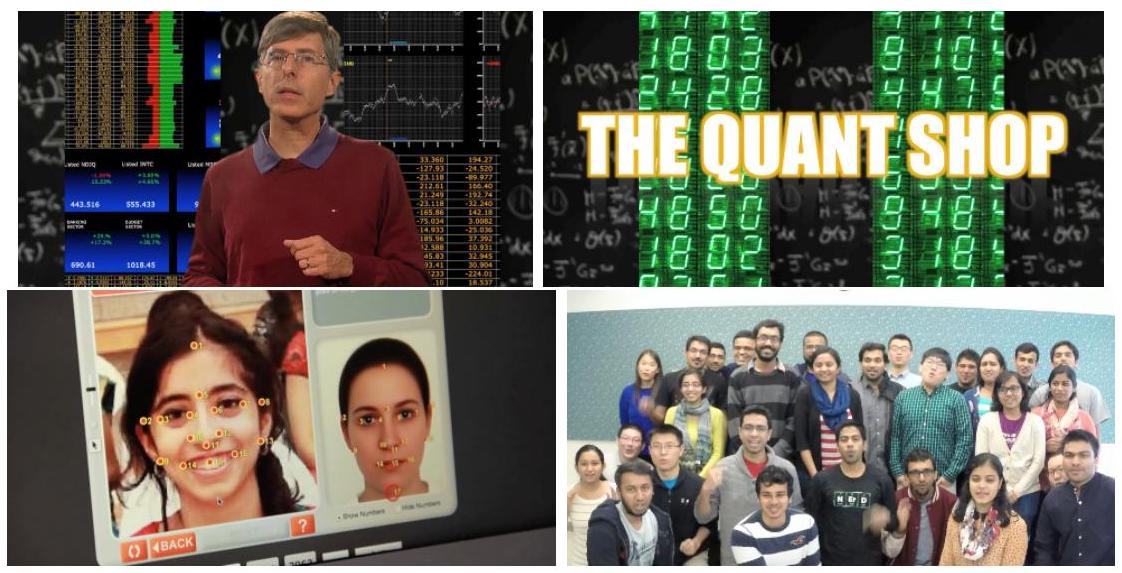
\includegraphics[max width=\textwidth]{2025_03_17_ca60ec0bfd96dcf8e028g-036}
\caption{Exciting scenes from data science television: The Quant Shop.}
\label{fig:1.8}
\end{figure}

\begin{itemize}
  \item \emph{Playing the Market} - Hedge fund quants get rich when guessing right about tomorrow's prices, and poor when wrong. How accurately can we predict future prices of gold and oil using histories of price data? What other information goes into building a successful price model?
\end{itemize}

I encourage you to watch some episodes of \emph{The Quant Shop} in tandem with reading this book. We try to make it fun, although I am sure you will find plenty of things to cringe at. Each show runs for thirty minutes, and maybe will inspire you to tackle a prediction challenge of your own.

These programs will certainly give you more insight into these eight specific challenges. I will use these projects throughout this book to illustrate important lessons in how to do data science, both as positive and negative examples. These projects provide a laboratory to see how intelligent but inexperienced people not wildly unlike yourself thought about a data science problem, and what happened when they did.

\subsubsection{Kaggle Challenges}
Another source of inspiration are challenges from Kaggle (\href{http://www.kaggle.com}{www.kaggle.com}), which provides a competitive forum for data scientists. New challenges are posted on a regular basis, providing a problem definition, training data, and a scoring function over hidden evaluation data. A leader board displays the scores of the strongest competitors, so you can see how well your model stacks up in comparison with your opponents. The winners spill their modeling secrets during post-contest interviews, to help you improve your modeling skills.

Performing well on Kaggle challenges is an excellent credential to put on your resume to get a good job as a data scientist. Indeed, potential employers will track you down if you are a real Kaggle star. But the real reason to participate is that the problems are fun and inspiring, and practice helps make you a better data scientist.

The exercises at the end of each chapter point to expired Kaggle challenges, loosely connected to the material in that chapter. Be forewarned that Kaggle provides a misleading glamorous view of data science as applied machine learning, because it presents extremely well-defined problems with the hard work of data collection and cleaning already done for you. Still, I encourage you to check it out for inspiration, and as a source of data for new projects.

\subsection{About the War Stories}
\emph{Genius} and \emph{wisdom} are two distinct intellectual gifts. Genius shows in discovering the right answer, making imaginative mental leaps which overcome obstacles and challenges. Wisdom shows in avoiding obstacles in the first place, providing a sense of direction or guiding light that keeps us moving soundly in the right direction.

Genius is manifested in technical strength and depth, the ability to see things and do things that other people cannot. In contrast, wisdom comes from experience and general knowledge. It comes from listening to others. Wisdom comes from humility, observing how often you have been wrong in the past and figuring out why you were wrong, so as to better recognize future traps and avoid them.

Data science, like most things in life, benefits more from wisdom than from genius. In this book, I seek to pass on wisdom that I have accumulated the hard way through \emph{war stories}, gleaned from a diverse set of projects I have worked on:

\begin{itemize}
  \item \emph{Large-scale text analytics and NLP:} My Data Science Laboratory at Stony Brook University works on a variety of projects in big data, including sentiment analysis from social media, historical trends analysis, deep learning approaches to natural language processing (NLP), and feature extraction from networks.
  \item \emph{Start-up companies:} I served as co-founder and chief scientist to two data analytics companies: General Sentiment and Thrivemetrics. General Sentiment analyzed large-scale text streams from news, blogs, and social media to identify trends in the sentiment (positive or negative) associated with people, places, and things. Thrivemetrics applied this type of analysis to internal corporate communications, like email and messaging systems.\\
Neither of these ventures left me wealthy enough to forgo my royalties from this book, but they did provide me with experience on cloud-based computing systems, and insight into how data is used in industry.
  \item \emph{Collaborating with real scientists:} I have had several interesting collaborations with biologists and social scientists, which helped shape my understanding of the complexities of working with real data. Experimental data is horribly noisy and riddled with errors, yet you must do the best you can with what you have, in order to discover how the world works.
  \item \emph{Building gambling systems:} A particularly amusing project was building a system to predict the results of jai-alai matches so we could bet on them, an experience recounted in my book \emph{Calculated Bets: Computers, Gambling, and Mathematical Modeling to Win}. Our system relied on web scraping for data collection, statistical analysis, simulation/modeling, and careful evaluation. We also have developed and evaluated predictive models for movie grosses, stock prices, and football games using social media analysis.
  \item \emph{Ranking historical figures:} By analyzing Wikipedia to extract meaningful variables on over 800,000 historical figures, we developed a scoring function to rank them by their strength as historical memes. This ranking does a great job separating the greatest of the great (Jesus, Napoleon, Shakespeare, Mohammad, and Lincoln round out the top five) from lesser mortals, and served as the basis for our book \emph{Who's Bigger?: Where Historical Figures Really Rank}.
\end{itemize}

All this experience drives what I teach in this book, especially the tales that I describe as war stories. \textit{Every one of these war stories is true.} Of course, the stories improve somewhat in the retelling, and the dialogue has been punched up to make them more interesting to read. However, I have tried to honestly trace the process of going from a raw problem to a solution, so you can watch how it unfolded.

\subsection{War Story: Answering the Right Question}
Our research group at Stony Brook University developed an NLP-based system for analyzing millions of news, blogs, and social media messages, and reducing this text to trends concerning all the entities under discussion. Counting the number of mentions each name receives in a text stream (volume) is easy, in principle. Determining whether the connotation of a particular reference is positive or negative (sentiment analysis) is hard. But our system did a pretty good job, particularly when aggregated over many references.

This technology served as the foundation for a social media analysis company named General Sentiment. It was exciting living through a start-up starting up, facing the challenges of raising money, hiring staff, and developing new products.

But perhaps the biggest problem we faced was answering the right question. The General Sentiment system recorded trends about the sentiment and volume for \emph{every} person, place, and thing that was ever mentioned in news, blogs, and social media: over 20 million distinct entities. We monitored the reputations of celebrities and politicians. We monitored the fates of companies and products. We tracked the performance of sports teams, and the buzz about movies. We could do anything!

But it turns out that no one pays you to do anything. They pay you to do \emph{something,} to solve a particular problem they have, or eliminate a specific pain point in their business. Being able to do anything proves to be a terrible sales strategy, because it requires you to find that need afresh for each and every customer.

Facebook didn't open up to the world until September 2006. So when General Sentiment started in 2008, we were at the very beginning of the social media era. We had lots of interest from major brands and advertising agencies which \emph{knew} that social media was ready to explode. They \emph{knew} this newfangled thing was important, and that they had to be there. They \emph{knew} that proper analysis of social media data could give them fresh insights into what their customers were thinking. But they didn't know exactly what it was they really wanted to know.

One aircraft engine manufacturer was very interested in learning how much the kids talked about them on Facebook. We had to break it to them gently that the answer was zero. Other potential customers demanded proof that we were more accurate than the Nielsen television ratings. But of course, if you wanted Nielsen ratings then you should buy them from Nielsen. Our system provided different insights from a completely different world. But you had to know what you wanted in order to use them.

We did manage to get substantial contracts from a very diverse group of customers, including consumer brands like Toyota and Blackberry, governmental organizations like the Hawaii tourism office, and even the presidential campaign of Republican nominee Mitt Romney in 2012. Our analysts provided them insights into a wide variety of business issues:

\begin{itemize}
  \item What did people think about Hawaii? (Answer: they think it is a very nice place to visit.)
  \item How quickly would Toyota's sentiment recover after news of serious brake problems in their cars? (Answer: about six months.)
  \item What did people think about Blackberry's new phone models? (Answer: they liked the iPhone much better.)
  \item How quickly would Romney's sentiment recover after insulting 47\% of the electorate in a recorded speech? (Answer: never.)
\end{itemize}

But each sale required entering a new universe, involving considerable effort and imagination on the part of our sales staff and research analysts. We never managed to get two customers in the same industry, which would have let us benefit from scale and accumulated wisdom.

Of course, the customer is always right. It was our fault that we could not explain to them the best way to use our technology. The lesson here is that the world will not beat a path to your door just for a new source of data. You must be able to supply the right questions before you can turn data into money.

\subsection{Chapter Notes}
The idea of using historical records from baseball players to establish that lefthanders have shorter lifespans is due to Halpern and Coren, but their conclusion remains controversial. The percentage of left-handers in the population has been rapidly growing, and the observed effects may be a function of survivorship bias. So lefties, hang in there! Full disclosure: I am one of you.

The discipline of quantitative baseball analysis is sometimes called \emph{sabermetrics}, and its leading light is a fellow named Bill James. I recommend budding data scientists read his \emph{Historical Baseball Abstract} as an excellent example of how one turns numbers into knowledge and understanding. Time Magazine once said of James: "Much of the joy of reading him comes from the extravagant spectacle of a first-rate mind wasting itself on baseball." I thank \href{http://sports-reference.com}{http://sports-reference.com} for permission to use images of their website in this book. Ditto to Amazon, the owner of IMDb.

The potential of ride-sharing systems in New York was studied by Santi et. al., who showed that almost 95\% of the trips could have been shared with no more than five minutes delay per trip.

The Lydia system for sentiment analysis is described in \cite{godbole2007large}. Methods to identify changes in word meaning through analysis of historical text corpora like Google Ngram are reported.

\subsection{Exercises}
\subsubsection{Identifying Data Sets}
1-1. [3] Identify where interesting data sets relevant to the following domains can be found on the web:\\
(a) Books.\\
(b) Horse racing.\\
(c) Stock prices.\\
(d) Risks of diseases.\\
(e) Colleges and universities.\\
(f) Crime rates.\\
(g) Bird watching.

For each of these data sources, explain what you must do to turn this data into a usable format on your computer for analysis.

1-2. [3] Propose relevant data sources for the following \emph{The Quant Shop} prediction challenges. Distinguish between sources of data that you are sure \emph{somebody} must have, and those where the data is clearly available to you.\\
(a) Miss Universe.\\
(b) Movie gross.\\
(c) Baby weight.\\
(d) Art auction price.\\
(e) White Christmas.\\
(f) Football champions.\\
(g) Ghoul pool.\\
(h) Gold/oil prices.

1-3. [3] Visit \href{http://data.gov}{http://data.gov}, and identify five data sets that sound interesting to you. For each write a brief description, and propose three interesting things you might do with them.

\subsubsection{Asking Questions}
1-4. [3] For each of the following data sources, propose three interesting questions you can answer by analyzing them:\\
(a) Credit card billing data.
```
%---- Page End Break Here ---- Page : 23
```latex
(b) Click data from \href{http://www.Amazon.com}{http://www.Amazon.com}\\
(c) White Pages residential/commercial telephone directory.

\begin{enumerate}
    \setcounter{enumi}{4}
    \item[\textbf{1-5.}] \textit{[5] } Visit Entrez, the National Center for Biotechnology Information (NCBI) portal. Investigate what data sources are available, particularly the Pubmed and Genome resources. Propose three interesting projects to explore with each of them.
    \item[\textbf{1-6.}] \textit{[5] } You would like to conduct an experiment to establish whether your friends prefer the taste of regular Coke or Diet Coke. Briefly outline a design for such a study.\\
    \item[\textbf{1-7.}] \textit{[5] } You would like to conduct an experiment to see whether students learn better if they study without any music, with instrumental music, or with songs that have lyrics. Briefly outline the design for such a study.
    \item[\textbf{1-8.}] \textit{[5] } Traditional polling operations like Gallup use a procedure called random digit dialing, which dials random strings of digits instead of picking phone numbers from the phone book. Suggest why such polls are conducted using random digit dialing.
\end{enumerate}

\section*{Implementation Projects}
\begin{enumerate}
    \setcounter{enumi}{8}
    \item[\textbf{1-9.}] \textit{[5] } Write a program to scrape the best-seller rank for a book on \href{http://Amazon.com}{Amazon.com}. Use this to plot the rank of all of Skiena's books over time. Which one of these books should be the next item that you purchase? Do you have friends for whom they would make a welcome and appropriate gift? :-)
    \item[\textbf{1-10.}] \textit{[5] } For your favorite sport (baseball, football, basketball, cricket, or soccer) identify a data set with the historical statistical records for all major participants. Devise and implement a ranking system to identify the best player at each position.
\end{enumerate}

\section*{Interview Questions}
\begin{enumerate}
    \setcounter{enumi}{10}
    \item [\textbf{1-11.}] \textit{[3] } For each of the following questions: 
    \begin{enumerate}
        \item produce a quick guess based only on your understanding of the world, and then 
        \item use Google to find supportable numbers to produce a more principled estimate from.
    \end{enumerate}
    How much did your two estimates differ by?
    \begin{enumerate}
        \item [(a)] How many piano tuners are there in the entire world?
        \item [(b)] How much does the ice in a hockey rink weigh?
        \item [(c)] How many gas stations are there in the United States?
        \item [(d)] How many people fly in and out of LaGuardia Airport every day?
        \item [(e)] How many gallons of ice cream are sold in the United States each year?
        \item [(f)] How many basketballs are purchased by the National Basketball Association (NBA) each year?
        \item [(g)] How many fish are there in all the world's oceans?
        \item [(h)] How many people are flying in the air right now, all over the world?
        \item [(i)] How many ping-pong balls can fit in a large commercial jet?
        \item [(j)] How many miles of paved road are there in your favorite country?
        \item [(k)] How many dollar bills are sitting in the wallets of all people at Stony Brook University?
        \item [(l)] How many gallons of gasoline does a typical gas station sell per day?
        \item [(m)] How many words are there in this book?
        \item [(n)] How many cats live in New York city?
        \item [(o)] How much would it cost to fill a typical car's gas tank with Starbucks's coffee?
        \item [(p)] How much tea is there in China?
        \item [(q)] How many checking accounts are there in the United States?
    \end{enumerate}
    \item[\textbf{1-12.}] \textit{[3] } What is the difference between regression and classification?\\
    \item[\textbf{1-13.}] \textit{[8] } How would you build a data-driven recommendation system? What are the limitations of this approach?\\
    \item[\textbf{1-14.}] \textit{[3] } How did you become interested in data science?\\
    \item[\textbf{1-15.}] \textit{[3] } Do you think data science is an art or a science?
\end{enumerate}

\section*{Kaggle Challenges}
\begin{enumerate}
    \item[1-16.] Who survived the shipwreck of the Titanic?\\ \href{https://www.kaggle.com/c/titanic}{https://www.kaggle.com/c/titanic}
    \item[1-17.] Where is a particular taxi cab going? \\ \href{https://www.kaggle.com/c/pkdd-15-predict-taxi-service-trajectory-i}{https://www.kaggle.com/c/pkdd-15-predict-taxi-service-trajectory-i}
    \item[1-18.] How long will a given taxi trip take? \\
    \href{https://www.kaggle.com/c/pkdd-15-taxi-trip-time-prediction-ii}{https://www.kaggle.com/c/pkdd-15-taxi-trip-time-prediction-ii}
\end{enumerate}

\section*{Chapter 2}

\section*{Mathematical Preliminaries}
A data scientist is someone who knows more statistics than a computer scientist and more computer science than a statistician.

\begin{itemize}
  \item Josh Blumenstock
\end{itemize}

You must walk before you can run. Similarly, there is a certain level of mathematical maturity which is necessary before you should be trusted to do anything meaningful with numerical data.

In writing this book, I have assumed that the reader has had some degree of exposure to probability\index{probability} and statistics, linear algebra, and continuous mathematics. I have also assumed that they have probably forgotten most of it, or perhaps didn't always see the forest (why things are important, and how to use them) for the trees (all the details of definitions, proofs, and operations).

This chapter will try to refresh your understanding of certain basic mathematical concepts. Follow along with me, and pull out your old textbooks if necessary for future reference. Deeper concepts will be introduced later in the book when we need them.

\subsection*{2.1 Probability}
Probability theory provides a formal framework for reasoning about the likelihood of events. Because it is a formal discipline, there are a thicket of associated definitions to instantiate exactly what we are reasoning about:

\begin{itemize}
  \item An \textit{experiment}\index{experiment} is a procedure which yields one of a set of possible outcomes. As our ongoing example, consider the experiment of tossing two six-sided dice, one red and one blue, with each face baring a distinct integer \{1, \ldots, 6\}.
  \item A \textit{sample space}\index{sample space} $S$ is the set of possible outcomes of an experiment. In our dice example, there are 36 possible outcomes, namely
\end{itemize}

\[
\begin{aligned}
S=\{ & (1,1),(1,2),(1,3),(1,4),(1,5),(1,6),(2,1),(2,2),(2,3),(2,4),(2,5),(2,6), \\
& (3,1),(3,2),(3,3),(3,4),(3,5),(3,6),(4,1),(4,2),(4,3),(4,4),(4,5),(4,6) \\
& (5,1),(5,2),(5,3),(5,4),(5,5),(5,6),(6,1),(6,2),(6,3),(6,4),(6,5),(6,6)\} .
\end{aligned}
\]

\begin{itemize}
  \item An \textit{event} $E$ is a specified subset of the outcomes of an experiment. The event that the sum of the dice equals 7 or 11 (the conditions to win at craps on the first roll) is the subset
\end{itemize}

\[
E=\{(1,6),(2,5),(3,4),(4,3),(5,2),(6,1),(5,6),(6,5)\}
\]

\begin{itemize}
  \item The \textit{probability} of an outcome $s$, denoted $p(s)$ is a number with the two properties:
  \item For each outcome $s$ in sample space $S, 0 \leq p(s) \leq 1$.
  \item The sum of probabilities of all outcomes adds to one: \(\sum_{s \in S} p(s)=1\).
\end{itemize}

If we assume two distinct fair dice, the probability \(p(s)=(1 / 6) \times(1 / 6)=1 / 36\) for all outcomes \(s \in S\).

\begin{itemize}
  \item The probability of an \textit{event} $E$ is the sum of the probabilities of the outcomes of the experiment. Thus
\end{itemize}

\[
p(E)=\sum_{s \in E} p(s)
\]

An alternate formulation is in terms of the complement of the event \(\bar{E}\), the case when $E$ does not occur. Then

\[
P(E)=1-P(\bar{E}) .
\]

This is useful, because often it is easier to analyze \(P(\bar{E})\) than \(P(E)\) directly.

\begin{itemize}
  \item A \textit{random variable} $V$ is a numerical function on the outcomes of a probability space. The function "sum the values of two dice" \(V((a, b))=a+b\) produces an integer result between 2 and 12. This implies a probability distribution of the values of the random variable. The probability \(P(V(s)=7)=1 / 6\), as previously shown, while \(P(V(s)=12)=1 / 36\).
  \item The \textit{expected value} of a random variable \(V\) defined on a sample space \(S\), \(E(V)\) is defined
\end{itemize}

\[
E(V)=\sum_{s \in S} p(s) \cdot V(s)
\]

All this you have presumably seen before. But it provides the language we will use to connect between probability and statistics. The data we see usually comes from measuring properties of observed events. The theory of probability and statistics provides the tools to analyze this data.

\subsection*{2.1.1 Probability vs. Statistics}
Probability and statistics are related areas of mathematics which concern themselves with analyzing the relative frequency of events. Still, there are fundamental differences in the way they see the world:

\begin{itemize}
  \item \textit{Probability} deals with predicting the likelihood of future events, while \textit{statistics} involves the analysis of the frequency of past events.

  \item Probability is primarily a theoretical branch of mathematics, which studies the consequences of mathematical definitions. \textit{Statistics} is primarily an applied branch of mathematics, which tries to make sense of observations in the real world.
\end{itemize}

Both subjects are important, relevant, and useful. But they are different, and understanding the distinction is crucial in properly interpreting the relevance of mathematical evidence. Many a gambler has gone to a cold and lonely grave for failing to make the proper distinction between probability and statistics.

This distinction will perhaps become clearer if we trace the thought process of a mathematician encountering her first craps game:

\begin{itemize}
  \item If this mathematician were a probabilist, she would see the dice and think "Six-sided dice? Each side of the dice is presumably equally likely to land face up. Now assuming that each face comes up with probability \(1 / 6\), I can figure out what my chances are of crapping out."

  \item If instead a statistician wandered by, she would see the dice and think "How do I know that they are not loaded? I'll watch a while, and keep track of how often each number comes up. Then I can decide if my observations are consistent with the assumption of equal-probability faces. Once I'm confident enough that the dice are fair, I'll call a probabilist to tell me how to bet."
\end{itemize}

In summary, probability theory enables us to find the consequences of a given ideal world, while statistical theory enables us to measure the extent to which our world is ideal. This constant tension between theory and practice is why statisticians prove to be a tortured group of individuals compared with the happy-go-lucky probabilists.

Modern probability theory first emerged from the dice tables of France in 1654. Chevalier de Méré, a French nobleman, wondered whether the player or the house had the advantage in a particular betting game. \footnote{He really shouldn't have wondered. The house always has the advantage.} In the basic version, the player rolls four dice, and wins provided none of them are a 6. The house collects on the even money bet if at least one 6 appears.

De Méré brought this problem to the attention of the French mathematicians Blaise Pascal and Pierre de Fermat, most famous as the source of Fermat's Last Theorem. Together, these men worked out the basics of probability theory,

\begin{figure}[h]
  \centering
  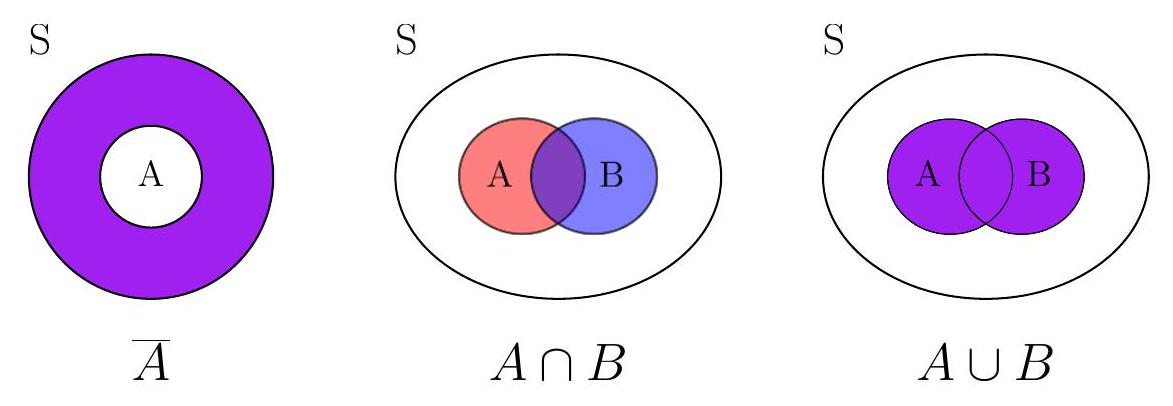
\includegraphics[max width=\textwidth]{2025_03_17_ca60ec0bfd96dcf8e028g-047}
  \caption{Venn diagrams illustrating set difference (left), intersection (middle), and union (right).}
\end{figure}

along the way establishing that the house wins this dice game with probability \(p=1-(5 / 6)^{4} \approx 0.517\), where the probability \(p=0.5\) would denote a fair game where the house wins exactly half the time.

\subsection*{2.1.2 Compound Events and independence\index{independence}}
We will be interested in complex events computed from simpler events $A$ and $B$ on the same set of outcomes. Perhaps event $A$ is that at least one of two dice be an even number, while event $B$ denotes rolling a total of either 7 or 11. Note that there exist certain outcomes of $A$ which are not outcomes of $B$, specifically

\[
\begin{aligned}
A-B=\{ & (1,2),(1,4),(2,1),(2,2),(2,3),(2,4),(2,6),(3,2),(3,6),(4,1) \\
& (4,2),(4,4),(4,5),(4,6),(5,4),(6,2),(6,3),(6,4),(6,6)\}
\end{aligned}
\]

This is the set difference operation. Observe that here \(B-A=\{\}\), because every pair adding to 7 or 11 must contain one odd and one even number.

The outcomes in common between both events $A$ and $B$ are called the intersection, denoted \(A \cap B\). This can be written as

\[
A \cap B=A-(S-B) .
\]

Outcomes which appear in either $A$ or $B$ are called the union, denoted \(A \cup B\). With the complement operation \(\bar{A}=S-A\), we get a rich language for combining events, shown in Figure 2.1. We can readily compute the probability of any of these sets by summing the probabilities of the outcomes in the defined sets.

The events $A$ and $B$ are independent if and only if

\[
P(A \cap B)=P(A) \times P(B)
\]

This means that there is no special structure of outcomes shared between events $A$ and $B$. Assuming that half of the students in my class are female, and half the students in my class are above average, we would expect that a quarter of my students are both female and above average if the events are independent.

\subsection*{2.1.3 conditional probability\index{conditional probability}}
When two events are correlated, there is a dependency between them which makes calculations more difficult. The conditional probability of $A$ given $B$, \(P(A \mid B)\) is defined:

\[
P(A \mid B)=\frac{P(A \cap B)}{P(B)}
\]

Recall the dice rolling events from Section 2.1.2 namely:

\begin{itemize}
  \item Event $A$ is that at least one of two dice be an even number.
  \item Event $B$ is the sum of the two dice is either a 7 or an 11 .
\end{itemize}

Observe that \(P(A \mid B)=1\), because any roll summing to an odd value must consist of one even and one odd number. Thus \(A \cap B=B\), analogous to the umbrella case above. For \(P(B \mid A)\), note that \(P(A \cap B)=9 / 36\) and \(P(A)=25 / 36\), so \(P(B \mid A)=9 / 25\).

Conditional probability will be important to us, because we are interested in the likelihood of an event $A$ (perhaps that a particular piece of email is spam) as a function of some evidence $B$ (perhaps the distribution of words within the document). Classification problems generally reduce to computing conditional probabilities, in one way or another.

Our primary tool to compute conditional probabilities will be Bayes theorem, which reverses the direction of the dependencies:

\[
P(B \mid A)=\frac{P(A \mid B) P(B)}{P(A)}
\]

Often it proves easier to compute probabilities in one direction than another, as in this problem. By Bayes theorem \(P(B \mid A)=(1 \cdot 9 / 36) /(25 / 36)=9 / 25\), exactly what we got before. We will revisit Bayes theorem in Section 5.6. where it will establish the foundations of computing probabilities in the face of evidence.

\begin{figure}[h]
  \centering
  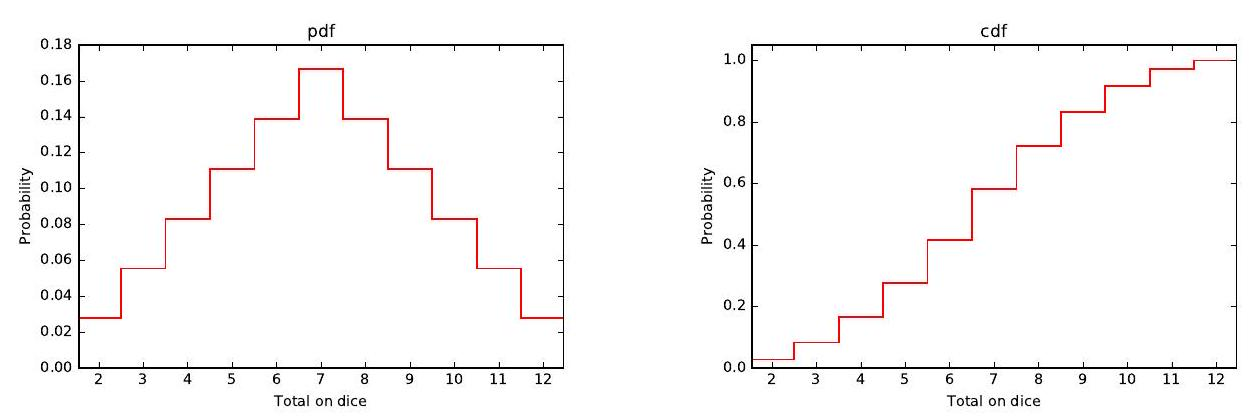
\includegraphics[max width=\textwidth]{2025_03_17_ca60ec0bfd96dcf8e028g-049}
  \caption{The probability density function (pdf) of the sum of two dice contains exactly the same information as the cumulative density function (cdf), but looks very different.}
\end{figure}

\subsection*{2.1.4 probability distribution\index{probability distribution}s}
Random variables are numerical functions where the values are associated with probabilities of occurrence. In our example where \(V(s)\) the sum of two tossed dice, the function produces an integer between 2 and 12. The probability of a particular value \(V(s)=X\) is the sum of the probabilities of all the outcomes which add up to \(X\).

Such random variables can be represented by their \textit{probability density function}, or pdf. This is a graph where the \(x\)-axis represents the range of values the random variable can take on, and the \(y\)-axis denotes the probability of that given value. Figure 2.2 (left) presents the pdf of the sum of two fair dice. Observe that the peak at \(X=7\) corresponds to the most frequent dice total, with a probability of \(1 / 6\).

Such pdf plots have a strong relationship to histograms of data frequency, where the \(x\)-axis again represents the range of value, but \(y\) now represents the observed frequency of exactly how many event occurrences were seen for each given value \(X\). Converting a histogram to a pdf can be done by dividing each bucket by the total frequency over all buckets. The sum of the entries then becomes 1, so we get a probability distribution.

Histograms are statistical: they reflect actual observations of outcomes. In contrast, pdfs are probabilistic: they represent the underlying chance that the next observation will have value \(X\). We often use the histogram of observations \(h(x)\) in practice to estimate the probabilities\footnote{A technique called discounting offers a better way to estimate the frequency of rare events, and will be discussed in Section 11.1 .2} by normalizing counts by the total number of observations:

\[
P(k=X)=\frac{h(k=X)}{\sum_{x} h(x=X)}
\]

There is another way to represent random variables which often proves useful, called a \textit{cumulative density function} or cdf. The cdf is the running sum of the probabilities in the pdf; as a function of \(k\), it reflects the probability that \(X \leq k\) instead of the probability that \(X=k\). Figure 2.2 (right) shows the cdf of the dice sum distribution. The values increase monotonically from left to right, because each term comes from adding a positive probability to the previous total. The rightmost value is 1, because all outcomes produce a value no greater than the maximum.

It is important to realize that the pdf \(P(V)\) and \texttt{cdf} \(C(V)\) of a given random variable \(V\) contain exactly the same information. We can move back and forth between them because:

\[
P(k=X)=C(X \leq k+\delta)-C(X \leq k)
\]

where \(\delta=1\) for integer distributions. The cdf is the running sum of the pdf, so

\[
C(X \leq k)=\sum_{x \leq k} P(X=x)
\]

Just be aware of which distribution you are looking at. Cumulative distributions always get higher as we move to the right, culminating with a probability of \(C(X \leq \infty)=1\). By contrast, the total area under the curve of a pdf equals 1, so the probability at any point in the distribution is generally substantially less.

\begin{figure}[h]
  \centering
  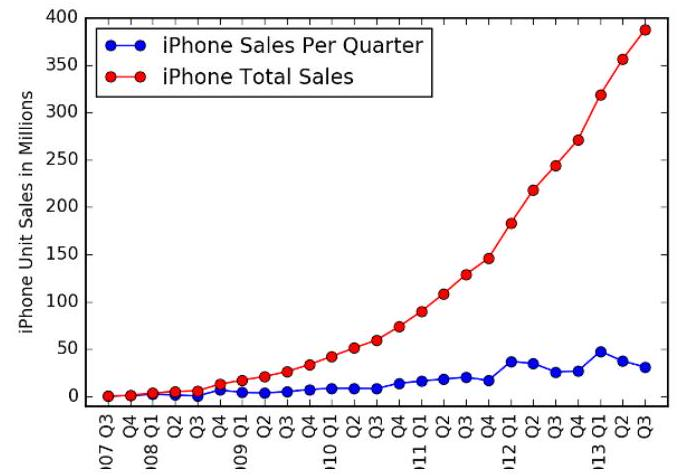
\includegraphics[max width=\textwidth]{2025_03_17_ca60ec0bfd96dcf8e028g-050}
  \caption{iPhone quarterly sales data presented as cumulative and incremental (quarterly) distributions. Which curve did Apple CEO Tim Cook choose to present?}
\end{figure}

\subsection*{2.2 Descriptive Statistics}
Descriptive statistics provide ways of capturing the properties of a given data set or sample. They summarize observed data, and provide a language to talk about it. Representing a group of elements by a new derived element, like mean, min, count, or sum reduces a large data set to a small summary statistic: aggregation as data reduction.

Such statistics can become features in their own right when taken over natural groups or clusters in the full data set. There are two main types of descriptive statistics:

\begin{itemize}
  \item \textit{Central tendency measures}, which capture the center around which the data is distributed.
  \item \textit{Variation} or \textit{variability measures}, which describe the data spread, i.e. how far the measurements lie from the center.
\end{itemize}

Together these statistics tell us an enormous amount about our distribution.

\subsection*{2.2.1 Centrality Measures}
The first element of statistics we are exposed to in school are the basic centrality measures: mean, median\index{median}, and mode. These are the right place to start when thinking of a single number to characterize a data set.

\begin{itemize}
  \item \textit{Mean}: You are probably quite comfortable with the use of the \textit{arithmetic} mean, where we sum values and divide by the number of observations:
\end{itemize}

\[
\mu_{X}=\frac{1}{n} \sum_{i=1}^{n} x_{i}
\]

We can easily maintain the mean under a stream of insertions and deletions, by keeping the sum of values separate from the frequency count, and divide only on demand.
The mean is very meaningful to characterize symmetric distributions without outliers, like height and weight. That it is symmetric means the number of items above the mean should be roughly the same as the number
below. That it is without outliers means that the range of values is reasonably tight. Note that a single MAXINT creeping into an otherwise sound set of observations throws the mean wildly off. The median is a centrality measure which proves more appropriate with such ill-behaved distributions.

\begin{itemize}
  \item \textit{geometric} mean\index{geometric mean}: The geometric mean is the \(n\)th root of the product of \(n\) values:
\end{itemize}

\[
\left(\prod_{i=1}^{n} a_{i}\right)^{1 / n}=\sqrt[n]{a_{1} a_{2} \ldots a_{n}}
\]

The geometric mean is always less than or equal to the arithmetic mean. For example, the geometric mean of the sums of 36 dice rolls is 6.5201, as opposed to the arithmetic mean of 7. It is very sensitive to values near zero. A single value of zero lays waste to the geometric mean: no matter what other values you have in your data, you end up with zero. This is somewhat analogous to having an outlier of \(\infty\) in an arithmetic mean.
But geometric means prove their worth when averaging ratios. The geometric mean of \(1 / 2\) and \(2 / 1\) is 1, whereas the mean is 1.25. There is less available "room" for ratios to be less than 1 than there is for ratios above 1, creating an asymmetry that the arithmetic mean overstates. The geometric mean is more meaningful in these cases, as is the arithmetic mean of the \textit{logarithms} of the ratios.

\begin{itemize}
  \item \textit{Median}: The median is the exact middle value among a data set; just as many elements lie above the median as below it. There is a quibble about what to take as the median when you have an even number of elements. You can take either one of the two central candidates: in any reasonable data set these two values should be about the same. Indeed in the dice example, both are 7.
A nice property of the median as so defined is that it must be a genuine value of the original data stream. There actually is someone of median height to you can point to as an example, but presumably no one in the world is of exactly average height. You lose this property when you average the two center elements.
Which centrality measure is best for applications? The median typically lies pretty close to the arithmetic mean in symmetrical distributions, but it is often interesting to see how far apart they are, and on which side of the mean the median lies.
The median generally proves to be a better statistic for skewed distributions or data with outliers: like wealth and income. Bill Gates adds $\$ 250$ to the mean per capita wealth in the United States, but nothing to the median. If he makes you personally feel richer, then go ahead and use the mean. But the median is the more informative statistic here, as it will be for any power law distribution.
\end{itemize}

\begin{figure}[h]
  \centering
  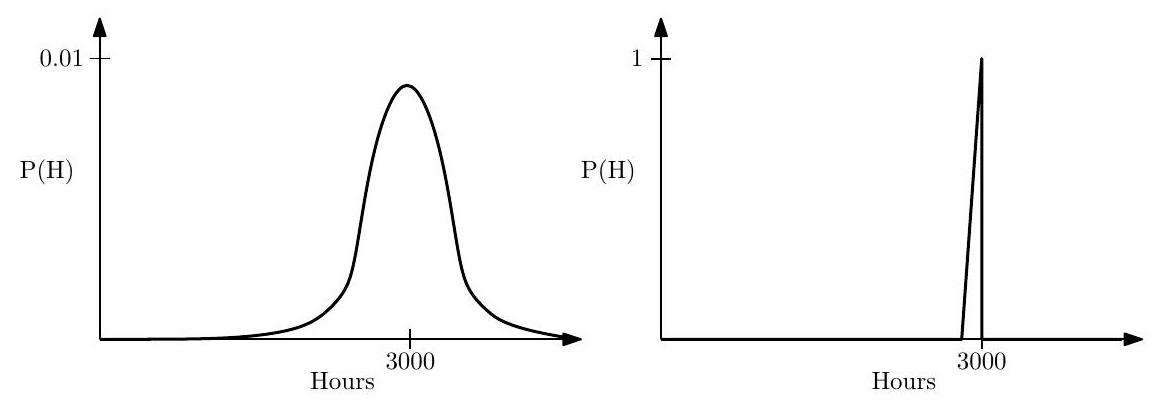
\includegraphics[max width=\textwidth]{2025_03_17_ca60ec0bfd96dcf8e028g-053}
  \caption{Two distinct probability distributions with \(\mu=3000\) for the lifespan of light bulbs: normal (left) and with zero variance\index{variance} (right).}
\end{figure}

\begin{itemize}
  \item \textit{mode}\index{mode}: The mode is the most frequent element in the data set. This is 7 in our ongoing dice example, because it occurs six times out of thirty-six elements. Frankly, I've never seen the mode as providing much insight as centrality measure, because it often isn't close to the center. Samples measured over a large range should have very few repeated elements or collisions at any particular value. This makes the mode a matter of happenstance. Indeed, the most frequently occurring elements often reveal artifacts or anomalies in a data set, such as default values or error codes that do not really represent elements of the underlying distribution.
The related concept of the peak in a frequency distribution (or histogram) is meaningful, but interesting peaks only get revealed through proper bucketing. The current peak of the annual salary distribution in the United States lies between $\$ 30,000$ and $\$ 40,000$ per year, although the mode presumably sits at zero.
\end{itemize}

\subsection*{2.2.2 variability measures\index{variability measures}}
The most common measure of variability is the \textit{standard deviation}\index{standard deviation} \(\sigma\), which measures sum of squares differences between the individual elements and the mean:

\[
\sigma=\sqrt{\frac{\sum_{i=1}^{n}\left(a_{i}-\bar{a}\right)^{2}}{n-1}}
\]

A related statistic, the \textit{variance} \(V\), is the square of the standard deviation, i.e. \(V=\sigma^{2}\). Sometimes it is more convenient to talk about variance than standard deviation, because the term is eight characters shorter. But they measure exactly the same thing.

As an example, consider the humble light bulb, which typically comes with an expected working life, say \(\mu=3000\) hours, derived from some underlying distribution shown in Figure 2.4. In a conventional bulb, the chance of it lasting longer than \(\mu\) is presumably about the same as that of it burning out quicker, and this degree of uncertainty is measured by \(\sigma\). Alternately, imagine a "printer cartridge bulb," where the evil manufacturer builds very robust bulbs, but includes a counter so they can prevent it from ever glowing after 3000 hours of use. Here \(\mu=3000\) and \(\sigma=0\). Both distributions have the same mean, but substantially different variance.

The sum of squares penalty in the formula for \(\sigma\) means that one outlier value \(d\) units from the mean contributes as much to the variance as \(d^{2}\) points each one unit from the mean, so the variance is very sensitive to outliers.

An often confusing matter concerns the denominator in the formula for standard deviation. Should we divide by \(n\) or \(n-1\)? The difference here is technical. The standard deviation of the full population divides by \(n\), whereas the standard deviation of the sample divides by \(n-1\). The issue is that sampling just one point tells us absolutely nothing about the underlying variance in any population, where it is perfectly reasonable to say there is zero variance in weight among the population of a one-person island. But for reasonable-sized data sets \(n \approx(n-1)\), so it really doesn't matter.

\subsection*{2.2.3 Interpreting Variance}
Repeated observations of the same phenomenon do not always produce the same results, due to random noise or error. \textit{Sampling errors} result when our observations capture unrepresentative circumstances, like measuring rush hour traffic on weekends as well as during the work week. \textit{Measurement errors} reflect the limits of precision inherent in any sensing device. The notion of \textit{signal to noise ratio}\index{signal to noise ratio} captures the degree to\index{interpretation} which a series of observations reflects a quantity of interest as opposed to data variance. As data scientists, we care about changes in the signal instead of the noise, and such variance often makes this problem surprisingly difficult.

I think of variance as an inherent property of the universe, akin to the speed of light or the time-value of money. Each morning you weigh yourself on a scale you are guaranteed to get a different number, with changes reflecting when you last ate (sampling error), the flatness of the floor, or the age of the scale (both measurement error) as much as changes in your body mass (actual variation). So what is your real weight?

Every measured quantity is subject to some level of variance, but the phenomenon cuts much deeper than that. Much of what happens in the world is just random fluctuations or arbitrary happenstance causing variance even when the situation is unchanged. Data scientists seek to explain the world through data, but distressingly often there is no real phenomena to explain, only a ghost created by variance. Examples include:

\begin{itemize}
  \item The \textit{stock market}\index{stock market}: Consider the problem of measuring the relative "skill" of different stock market investors. We know that Warren Buffet is much better at investing than we are. But very few professional investors prove consistently better than others. Certain investment vehicles wildly outperform the market in any given time period. However, the hot fund one
\end{itemize}

\begin{verbatim}
ln[28]:= Season[p_Real, n_Integer] :=
    Count[Table[If[RandomReal[1] }\leqslantP,1,0],{n}], 1]/(1.0*n
In[29]:= Histogram[d = Table[Season[0.300, 500], {100 000}], 100]
\end{verbatim}

\begin{figure}[h]
  \centering
  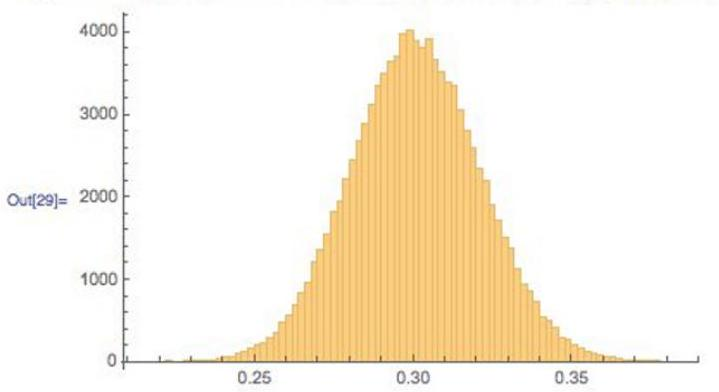
\includegraphics[max width=\textwidth]{2025_03_17_ca60ec0bfd96dcf8e028g-055}
  \caption{Sample variance on hitters with a real 30\% success rate results in a wide range of observed performance even over 500 trials per season.}
\end{figure}

year usually underperforms the market the year after, which shouldn't happen if this outstanding performance was due to skill rather than luck.

The fund managers themselves are quick to credit profitable years to their own genius, but losses to unforeseeable circumstances. However, several studies have shown that the performance of professional investors is essentially random, meaning there is little real difference in skill. Most investors are paying managers for previously-used luck. So why do these entrail-readers get paid so much money?

\begin{itemize}
  \item \textit{sports performance}\index{sports performance}: Students have good semesters and bad semesters, as reflected by their grade point average (GPA). Athletes have good and bad seasons, as reflected by their performance and statistics. Do such changes reflect genuine differences in effort and ability, or are they just variance?
In baseball, .300 hitters (players who hit with a 30\% success rate) represent consistency over a full season. Batting .275 is not a noteworthy season, but hit .300 and you are a star. Hit . 325 and you are likely to be the batting champion.
\end{itemize}

Figure 2.5 shows the results of a simple simulation, where random numbers were used to decide the outcome of each at-bat over a 500 at-bats/season. Our synthetic player is a real .300 hitter, because we programmed it to report a hit with probability 300 / 1000 (0.3). The results show that a real . 300 hitter has a 10\% chance of hitting .275 or below, just by chance. Such a season will typically be explained away by injuries or maybe the inevitable effects of age on athletic performance. But it could just be natural variance. Smart teams try to acquire a good hitter after a lousy season, when the price is cheaper, trying to take advantage of this variance.

Our . 300 hitter also has a 10\% chance of batting above .325
```
%---- Page End Break Here ---- Page : 38
\

\section{Characterizing distributions}
Distributions do not necessarily have much probability mass exactly at the mean. Consider what your wealth would look like after you borrow \$100 million, and then bet it all on an even money coin flip. Heads you are now \$100 million in clear, tails you are \$100 million in hock. Your expected wealth is zero, but this mean does not tell you much about the shape of your wealth distribution.

However, taken together the mean and standard deviation do a decent job of characterizing \textit{any} distribution. Even a relatively small amount of mass positioned far from the mean would add a lot to the standard deviation, so a small value of \(\sigma\) implies the bulk of the mass must be near the mean.

To be precise, regardless of how your data is distributed, at least \((1-(1/k^{2}))\)th of the mass must lie within \(\pm k\) standard deviations of the mean. This means that at least 75\% of all the data must lie within \(2\sigma\) of the mean, and almost 89\% within \(3\sigma\) for any distribution.

We will see that even tighter bounds hold when we know the distribution is well-behaved, like the Gaussian or normal distribution. But this is why it is a great practice to report both \(\mu\) and \(\sigma\) whenever you talk about averages. The average height of adult women in the United States is \(63.7 \pm 2.7\) inches, meaning \(\mu=63.7\) and \(\sigma=2.7\). The average temperature in Orlando, Fl is 60.3 degrees Fahrenheit. However, there have been many more 100 degree days at Disney World than 100 inch (8.33 foot) women visiting to enjoy them.

\textbf{Take-Home Lesson:} Report both the mean and standard deviation to characterize your distribution, written as \(\mu \pm \sigma\).

\section{Correlation Analysis}
Suppose we are given two variables \(x\) and \(y\), represented by a sample of \(n\) points of the form \((x_{i}, y_{i})\), for \(1 \leq i \leq n\). We say that \(x\) and \(y\) are \textit{correlated} when the value of \(x\) has some predictive power on the value of \(y\).

The \textit{correlation coefficient} \(r(X, Y)\) is a statistic that measures the degree to which \(Y\) is a function of \(X\), and vice versa. The value of the correlation coefficient ranges from -1 to 1, where 1 means fully correlated and 0 implies no relation, or independent variables. Negative correlations imply that the variables are \textit{anti-correlated}, meaning that when \(X\) goes up, \(Y\) goes down.

Perfectly anti-correlated variables have a correlation of -1. Note that negative correlations are just as good for predictive purposes as positive ones. That you are less likely to be unemployed the more education you have is an example of a negative correlation, so the level of education can indeed help predict job status. Correlations around 0 are useless for forecasting.

Observed correlations drive many of the predictive models we build in data science. Representative strengths of correlations include:
\begin{itemize}
    \item Are taller people more likely to remain lean? The observed correlation between height and BMI is \(r=-0.711\), so height is indeed negatively correlated with body mass index (BMI).\footnote{\url{https://onlinecourses.science.psu.edu/stat500/node/60}}
    \item Do standardized tests predict the performance of students in college? The observed correlation between SAT scores and freshmen GPA is \(r=0.47\), so yes, there is some degree of predictive power. But social economic status is just as strongly correlated with SAT scores \((r=0.42)\).\footnote{\url{https://research.collegeboard.org/sites/default/files/publications/2012/9/researchreport-2009-1-socioeconomic-status-sat-freshman-gpa-analysis-data.pdf}}
    \item Does financial status affect health? The observed correlation between household income and the prevalence of coronary artery disease is \(r= -0.717\), so there is a strong negative correlation. So yes, the wealthier you are, the lower your risk of having a heart attack.\footnote{\url{http://www.ncbi.nlm.nih.gov/pmc/articles/PMC3457990/}}
    \item Does smoking affect health? The observed correlation between a group's propensity to smoke and their mortality rate is \(r=0.716\), so for G-d's sake, don't smoke.\footnote{\url{http://lib.stat.cmu.edu/DASL/Stories/SmokingandCancer.html}}
    \item Do violent video games increase aggressive behavior? The observed correlation between play and violence is \(r=0.19\), so there is a weak but significant correlation.\footnote{\url{http://webspace.pugetsound.edu/facultypages/cjones/chidev/Paper/Articles/Anderson-Aggression.pdf}}
\end{itemize}

This section will introduce the primary measurements of correlation. Further, we study how to appropriately determine the strength and power of any observed correlation, to help us understand when the connections between variables are real.

\subsection{Correlation Coefficients: Pearson and Spearman Rank}
In fact, there are two primary statistics used to measure correlation. Mercifully, both operate on the same -1 to 1 scale, although they measure somewhat different things. These different statistics are appropriate in different situations, so you should be aware of both of them.

\subsubsection{The Pearson Correlation Coefficient}
The more prominent of the two statistics is \textit{Pearson correlation}, defined as
\[
r=\frac{\sum_{i=1}^{n}\left(X_{i}-\bar{X}\right)\left(Y_{i}-\bar{Y}\right)}{\sqrt{\sum_{i=1}^{n}\left(X_{i}-\bar{X}\right)^{2}} \sqrt{\sum_{i=1}^{n}\left(Y_{i}-\bar{Y}\right)^{2}}}=\frac{\operatorname{Cov}(X, Y)}{\sigma(X) \sigma(Y)}
\]

Let's parse this equation. Suppose \(X\) and \(Y\) are strongly correlated. Then we would expect that when \(x_{i}\) is greater than the mean \(\bar{X}\), then \(y_{i}\) should be bigger than its mean \(\bar{Y}\). When \(x_{i}\) is lower than its mean, \(y_{i}\) should follow. Now look at the numerator. The sign of each term is positive when both values are above (1 \times 1) or below (-1 \times-1) their respective means. The sign of each term is negative ((-1 \times 1) or (1 \times-1)) if they move in opposite directions, suggesting negative correlation. If \(X\) and \(Y\) were uncorrelated, then positive and negative terms should occur with equal frequency, offsetting each other and driving the value to zero.

The numerator's operation determining the sign of the correlation is so useful that we give it a name, \textit{covariance}, computed:
\[
\operatorname{Cov}(X, Y)=\sum_{i=1}^{n}\left(X_{i}-\bar{X}\right)\left(Y_{i}-\bar{Y}\right)
\]

Remember covariance: we will see it again in Section 8.2.3. The denominator of the Pearson formula reflects the amount of variance in the two variables, as measured by their standard deviations. The covariance between \(X\) and \(Y\) potentially increases with the variance of these variables, and this denominator is the magic amount to divide it by to bring correlation to a -1 to 1 scale.

\begin{figure}[h]
    \centering
    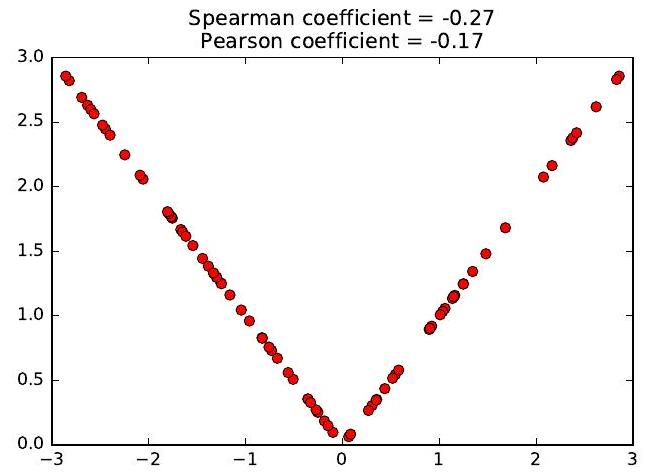
\includegraphics[max width=\textwidth]{2025_03_17_ca60ec0bfd96dcf8e028g-059}
    \caption{The function \(y=|x|\) does not have a linear model, but seems like it should be easily fitted despite weak correlations.}
\end{figure}

\subsubsection{The Spearman Rank Correlation Coefficient}
The Pearson correlation coefficient defines the degree to which a linear predictor of the form \(y=m \cdot x+b\) can fit the observed data. This generally does a good job measuring the similarity between the variables, but it is possible to construct pathological examples where the correlation coefficient between \(X\) and \(Y\) is zero, yet \(Y\) is completely dependent on (and hence perfectly predictable from) \(X\).

Consider points of the form \((x,|x|)\), where \(x\) is uniformly (or symmetrically) sampled from the interval \([-1,1]\) as shown in Figure 2.6. The correlation will be zero because for every point \((x, x)\) there will be an offsetting point \((-x, x)\), yet \(y=|x|\) is a perfect predictor. Pearson correlation measures how well the best linear predictors can work, but says nothing about weirder functions like absolute value.

The \textit{Spearman rank correlation coefficient} essentially counts the number of pairs of input points which are out of order. Suppose that our data set contains points \((x_{1}, y_{1})\) and \((x_{2}, y_{2})\) where \(x_{1}<x_{2}\) and \(y_{1}<y_{2}\). This is a vote that the values are positively correlated, whereas the vote would be for a negative correlation if \(y_{2}<y_{1}\).

Summing up over all pairs of points and normalizing properly gives us Spearman rank correlation. Let \(\operatorname{rank}\left(x_{i}\right)\) be the rank of \(x_{i}\) in sorted order among all \(x_{i}\), so the rank of the smallest value is 1 and the largest value \(n\). Then
\[
\rho=1-\frac{6 \sum d_{i}^{2}}{n\left(n^{2}-1\right)}
\]
where \(d_{i}=\operatorname{rank}\left(x_{i}\right)-\operatorname{rank}\left(y_{i}\right)\).

The relationship between our two coefficients is better delineated by the example in Figure 2.7. In addition to giving high scores to non-linear but monotonic functions, Spearman correlation is less sensitive to extreme outlier elements than Pearson. Let \(p=(x_{1}, y_{\max})\) be the data point with largest value.

\begin{figure}[h]
    \centering
    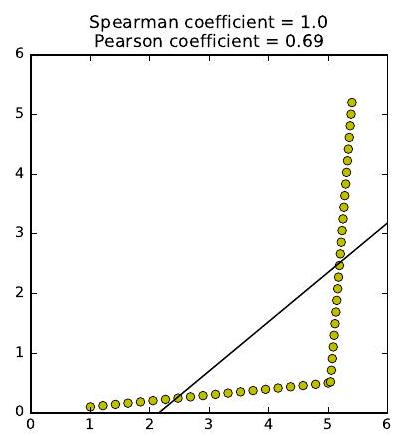
\includegraphics[max width=\textwidth]{2025_03_17_ca60ec0bfd96dcf8e028g-060(2)}
    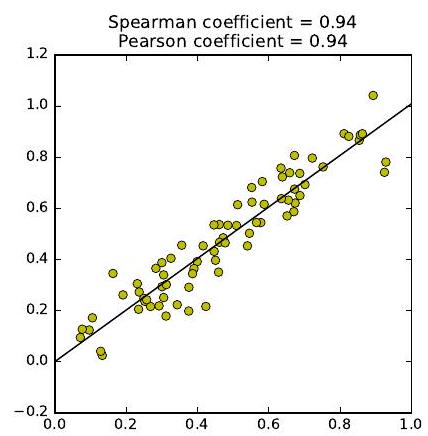
\includegraphics[max width=\textwidth]{2025_03_17_ca60ec0bfd96dcf8e028g-060}
    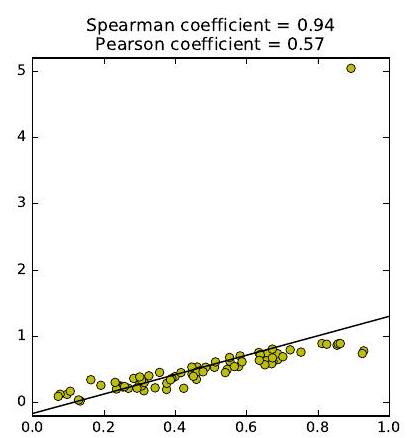
\includegraphics[max width=\textwidth]{2025_03_17_ca60ec0bfd96dcf8e028g-060(1)}
    \caption{A monotonic but not linear point set has a Spearman coefficient \(r=1\) even though it has no good linear fit (left). Highly-correlated sequences are recognized by both coefficients (center), but the Pearson coefficient is much more sensitive to outliers (right).}
\end{figure}

%---- Page End Break Here ---- Page : 58
\begin{itemize}
  \item \textit{Java and C/C++}: These mainstream programming languages for the development of large systems are important in big data applications. Parallel processing systems like Hadoop and Spark are based on Java and C++, respectively. If you are living in the world of distributed computing, then you are living in a world of Java and C++ instead of the other languages listed here.
  
  \item \textit{Mathematica/Wolfram Alpha}: Mathematica is a proprietary system providing computational support for all aspects of numerical and symbolic mathematics, built upon the less proprietary Wolfram programming language. It is the foundation of the Wolfram Alpha computational knowledge engine, which processes natural language-like queries through a mix of algorithms and pre-digested data sources. Check it out at \href{http://www.wolframalpha.com}{wolframalpha.com}.\\
I will confess a warm spot for Mathematica. It is what I tend to reach for when I am doing a small data analysis or simulation, but cost has traditionally put it out of the range of many users. The release of the Wolfram language perhaps now opens it up to a wider community.
  
  \item \textit{Excel}: Spreadsheet programs like Excel are powerful tools for exploratory data analysis, such as playing with a given data set to see what it contains. They deserve our respect for such applications.\\
Full featured spreadsheet programs contain a surprising amount of hidden functionality for power users. A student of mine who rose to become a Microsoft executive told me that 25\% of all new feature requests for Excel proposed functionality already present there. The special functions and data manipulation features you want probably are in Excel if you look hard enough, in the same way that a Python library for what you need probably will be found if you search for it.
\end{itemize}

\subsection{The Importance of Notebook Environments}
The primary deliverable for a data science project should not be a program. It should not be a data set. It should not be the results of running the program on your data. It should not just be a written report.

The deliverable result of every data science project should be a computable notebook tying together the code, data, computational results, and written analysis of what you have learned in the process. Figure~\ref{fig:jupyter} presents an excerpt from a Jupyter/IPython notebook, showing how it integrates code, graphics, and documentation into a descriptive document which can be executed like a program.

The reason this is so important is that computational results are the product of long chains of parameter selections and design decisions. This creates several problems that are solved by notebook computing environments:

\begin{verbatim}
# Example of a notebook code block
degrees = range(1, 8)
errors = np.array([regressor3(d) for d in degrees])
plt.plot(degrees, errors[:, 0], marker='^', c='r', label='Testing samples')
plt.plot(degrees, errors[:, 1], marker='o', c='b', label='Training samples')
plt.yscale('log')
plt.xlabel("degree")
plt.ylabel("Error")
plt.legend(loc='best')
\end{verbatim}

\begin{figure}[h]
\centering
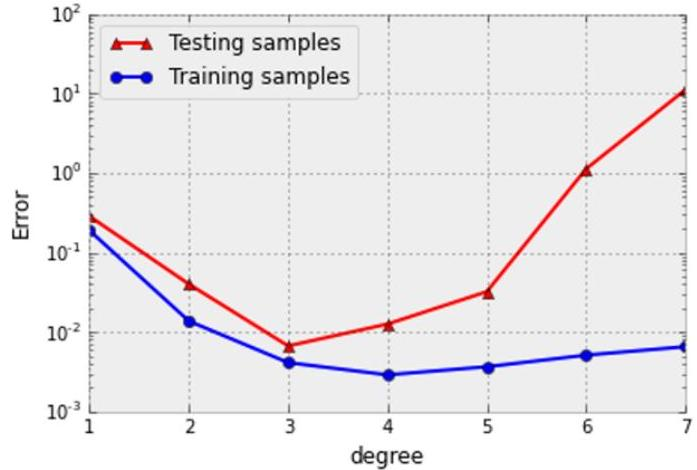
\includegraphics[max width=\textwidth]{2025_03_17_ca60ec0bfd96dcf8e028g-077}
\caption{Jupyter/IPython notebooks tie together code, computational results, and documentation.}
\label{fig:jupyter}
\end{figure}

By sweeping the degree, we discover two regions of model performance:
\begin{itemize}
  \item \textit{Underfitting (degree < 3)}: Characterized by the fact that the testing error will get lower if we increase the model capacity.
  \item \textit{Overfitting (degree > 3)}: Characterized by the fact the testing error will get higher if we increase the model capacity. Note that the training error is getting lower or just staying the same!
\end{itemize}

\begin{itemize}
  \item \textit{Computations need to be reproducible.} We must be able to run the same programs again from scratch, and get exactly the same result. This means that data pipelines must be \textit{complete}: taking raw input and producing the final output. It is terrible karma to start with a raw data set, do some processing, edit/format the data files by hand, and then do some more processing—because what you did by hand cannot be readily done again on another data set, or undone after you realize that you may have goofed up.
  \item \textit{Computations must be tweakable.} Often reconsideration or evaluation will prompt a change to one or more parameters or algorithms. This requires rerunning the notebook to produce the new computation. There is nothing more disheartening than to be given a big data product without provenance and told that \textit{this} is the final result and you can't change anything. A notebook is never finished until after the entire project is done.
  \item \textit{Data pipelines need to be documented.} That notebooks permit you to integrate text and visualizations with your code provides a powerful way to communicate what you are doing and why, in ways that traditional programming environments cannot match.
\end{itemize}

\textit{Take-Home Lesson}: Use a notebook environment like IPython or Mathematica to build and report the results of any data science project.

\subsection{Standard Data Formats}
Data comes from all sorts of places, and in all kinds of formats. Which representation is best depends upon who the ultimate consumer is. Charts and graphs are marvelous ways to convey the meaning of numerical data to people. Indeed, Chapter 6 will focus on techniques for visualizing data. But these pictures are essentially useless as a source of data to compute with. There is a long way from printed maps to Google Maps.

The best computational data formats have several useful properties:
\begin{itemize}
  \item \textit{They are easy for computers to parse:} Data written in a useful format is destined to be used again, elsewhere. Sophisticated data formats are often supported by APIs that govern technical details ensuring proper format.
  \item \textit{They are easy for people to read:} Eyeballing data is an essential operation in many contexts. Which of the data files in this directory is the right one for me to use? What do we know about the data fields in this file? What is the gross range of values for each particular field?\\
These use cases speak to the enormous value of being able to open a data file in a text editor to look at it. Typically, this means presenting the data in a human-readable text-encoded format, with records demarcated by separate lines, and fields separated by delimiting symbols.
  \item \textit{They are widely used by other tools and systems:} The urge to invent proprietary data standard beats firmly in the corporate heart, and most software developers would rather share a toothbrush than a file format. But these are impulses to be avoided. The power of data comes from mixing and matching it with other data resources, which is best facilitated by using popular standard formats.
\end{itemize}

One property I have omitted from this list is \textit{conciseness}, since it is generally not a primary concern for most applications running on modern computing systems. The quest to minimize data storage costs often works against other goals. Cleverly packing multiple fields into the higher-order bits of integers saves space, but at the cost of making it incompatible and unreadable.

The most important data formats/representations to be aware of are discussed below:
\begin{itemize}
  \item \textit{CSV (comma separated value) files:} These files provide the simplest, most popular format to exchange data between programs. That each line represents a single record, with fields separated by commas, is obvious from inspection. But subtleties revolve around special characters and text strings: what if your data about names contains a comma, like "Thurston Howell, Jr." The csv format provides ways to escape code such characters so they are not treated as delimiters, but it is messy. A better alternative is to use a rarer delimiter character, as in tsv or \textit{tab separated value} files.\\
The best test of whether your csv file is properly formatted is whether Microsoft Excel or some other spreadsheet program can read it without hassle. Make sure the results of every project pass this test as soon as the first csv file has been written, to avoid pain later.
  
  \item \textit{XML (eXtensible Markup Language):} Structured but non-tabular data are often written as text with annotations. The natural output of a named-entity tagger for text wraps the relevant substrings of a text in brackets denoting person, place, or thing. I am writing this book in LaTex, a formatting language with bracketing commands positioned around mathematical expressions and \textit{italicized text}. All webpages are written in HTML, the hypertext markup language which organizes documents using bracketing commands like \texttt{<b>} and \texttt{</b>} to enclose \textbf{bold faced text}.\\
XML is a language for writing specifications of such markup languages. A proper XML specification enables the user to parse any document complying with the specification. Designing such specifications and fully adhering to them requires discipline, but is worthwhile. In the first version of our Lydia text analysis system, we wrote our markups in a "pseudo-XML," read by ad hoc parsers that handled 99\% of the documents correctly but broke whenever we tried to extend them. After a painful switch to XML, everything worked more reliably \textit{and} more efficiently, because we could deploy fast, open-source XML parsers to handle all the dirty work of enforcing our specifications.
  
  \item \textit{SQL (structured query language) databases:} Spreadsheets are naturally structured around single tables of data. In contrast, relational databases prove excellent for manipulating multiple distinct but related tables, using SQL to provide a clunky but powerful query language.\\
Any reasonable database system imports and exports records as either csv or XML files, as well as an internal content dump. The internal representation in databases is opaque, so it really isn't accurate to describe them as a data format. Still, I emphasize them here because SQL databases generally prove a better and more powerful solution than manipulating multiple data files in an ad hoc manner.
  
  \item \textit{JSON (JavaScript Object Notation):} This is a format for transmitting data objects between programs. It is a natural way to communicate the state of variables/data structures from one system to another. This representation is basically a list of attribute-value pairs corresponding to variable/field names, and the associated values:
\begin{verbatim}
{"employees":[
    {"firstName":"John", "lastName":"Doe"},
    {"firstName":"Anna", "lastName":"Smith"},
    {"firstName":"Peter", "lastName":"Jones"}
]}
\end{verbatim}
Because library functions that support reading and writing JSON objects are readily available in all modern programming languages, it has become a very convenient way to store data structures for later use. JSON objects are human readable, but are quite cluttered-looking, representing arrays of records compared to CSV files. Use them for complex structured objects, but not simple tables of data.
  
  \item \textit{Protocol buffers:} These are a language/platform-neutral way of serializing structured data for communications and storage across applications. They are essentially lighter weight versions of XML (where you define the format of your structured data), designed to communicate small amounts of data across programs like JSON. This data format is used for much of the intermachine communication at Google. Apache Thrift is a related standard, used at Facebook.
\end{itemize}
%---- Page End Break Here ---- Page : 68
%---- Page End Break Here ---- Page : 68

thousand characters), this device in principle has room for 3 billion records, roughly one for every two people on earth.

The important considerations in designing any logging system are:

\begin{itemize}
  \item Build it to endure with limited maintenance. Set it and forget it, by provisioning it with enough storage for unlimited expansion, and a backup.
  \item Store all fields of possible value, without going crazy.
  \item Use a human-readable format or transactions database, so you can understand exactly what is in there when the time comes, months or years later, to sit down and analyze your data.
\end{itemize}

\subsection{Cleaning Data}
\index{cleaning data}
"garbage in, garbage out\index{garbage in, garbage out}" is the fundamental principle of data analysis. The road from raw data to a clean, analyzable data set can be a long one.

Many potential issues can arise in cleaning data for analysis. In this section, we discuss identifying processing artifacts\index{artifacts} and integrating diverse data sets. Our focus here is the processing \emph{before} we do our real analysis, to make sure that the garbage never gets in in the first place.

\emph{Take-Home Lesson:} Savvy painting restorers only do things to the original that are reversible. They never do harm. Similarly, data cleaning is always done on a copy of the original data, ideally by a pipeline that makes changes in a systematic and repeatable way.

\subsubsection{Errors vs. Artifacts}
\index{errors vs. artifacts}
Under ancient Jewish law, if a suspect on trial was unanimously found guilty by all judges, then this suspect would be \emph{acquitted}. The judges had noticed that unanimous agreement often indicates the presence of a systemic error in the judicial process. They reasoned that when something seems too good to be true, a mistake has likely been made somewhere.

If we view data items as measurements about some aspect of the world, data \emph{errors} represent information that is fundamentally lost in acquisition. The Gaussian noise blurring the resolution of our sensors represents error, precision which has been permanently lost. The two hours of missing logs because the server crashed represents data error: it is information which cannot be reconstructed again.

By contrast, \emph{artifacts} are generally systematic problems arising from processing done to the raw information it was constructed from. The good news is that processing artifacts can be corrected, so long as the original raw data set remains available. The bad news is that these artifacts must be detected before they can be corrected.

%---- Page End Break Here ---- Page : 69

\begin{figure}[ht]
  \centering
  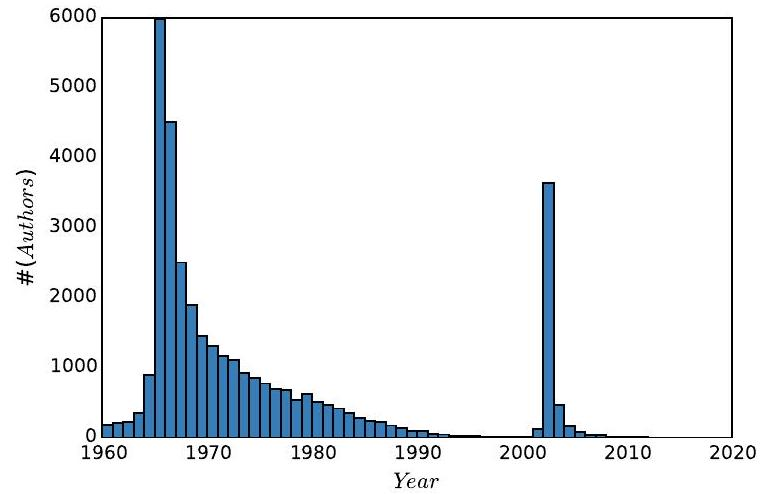
\includegraphics[max width=\textwidth]{2025_03_17_ca60ec0bfd96dcf8e028g-087}
  \caption{What artifacts can you find in this time series, counting the number of author's names first appearing in the scientific literature each year?}
\end{figure}

The key to detecting processing artifacts is the "sniff test," examining the product closely enough to get a whiff of something bad. Something bad is usually something unexpected or surprising, because people are naturally optimists. Surprising observations are what data scientists live for. Indeed, such insights are the primary reason we do what we do. But in my experience, most surprises turn out to be artifacts, so we must look at them skeptically.

Figure \ref{fig:artifact-detection} presents computational results from a project where we investigated the process of scientific publication. It shows a time series of the 100,000 most prolific authors, binned according to the year of their first paper appearing in Pubmed\index{Pubmed}, an essentially complete bibliography of the biomedical literature.

Study this figure closely, and see if you can discover any artifacts worth commenting on. I see at least two of them. Extra credit will be awarded if you can figure out what caused the problem.

The key to finding artifacts is to look for anomalies in the data, that contradict what you expect to see. What \emph{should} the distribution in the number of virgin authors look like, and how should it change over time? First, construct a prior distribution of what you expect to see, so that you can then properly evaluate potential anomalies against it.

My intuition says that the distribution of new top scientists should be pretty flat, because new stars are born with every successive class of graduate students. I would also guess that there may be a gradual drift upward as population expands, and more people enter the scientific community. But that's not what I see in Figure \ref{fig:artifact-detection}. So try to enumerate what the anomalies/potential artifacts are...

I see two big bumps when I look at Figure \ref{fig:artifact-detection}: a left bump starting around 1965, and a peak which explodes in 2002. On reflection, the leftmost bump makes sense. This left peak occurs the year when Pubmed first started to systematically collect bibliographic records. Although there is some very incomplete data from 1960–1964, most older scientists who had been publishing papers for several years would "emerge" only with the start of systematic records in 1965. So this explains the left peak, which then settles down by 1970 to what looks like the flat distribution we expected.

But what about that giant 2002 peak? And the decline in new authors to almost zero in the years which precede it? A similar decline is also visible to the right of the big peak. Were all the world's major scientists destined to be born in 2002?

A careful inspection of the records in the big peak revealed the source of the anomaly: first names. In the early days of Pubmed, authors were identified by their initials and last names. But late in 2001, \emph{SS Skiena} became \emph{Steven S. Skiena}, so it looked like a new author emerging from the heavens.

But why the declines to nothingness to the left and right of this peak? Recall that we limited this study to the 100,000 most prolific scientists. A scientific rock star emerging in 1998 would be unlikely to appear in this ranking because their name was doomed to change a few years later, not leaving enough time to accumulate a full career of papers. Similar things happen at the very right of the distribution: newly created scientists in 2010 would never be able to achieve a full career's work in only a couple of years. Both phenomena are neatly explained by this first name basis.

Cleaning this data to unify name references took us a few iterations to get right. Even after eliminating the 2002 peak, we still saw a substantial dip in prominent scientists starting their careers in the mid-1990s. This was because many people who had a great half career pre-first names and a second great half career post-first names did not rise to the threshold of a great full career in either single period. Thus we had to match all the names in the full before identifying who were the top 100,000 scientists.

\begin{figure}[ht]
  \centering
  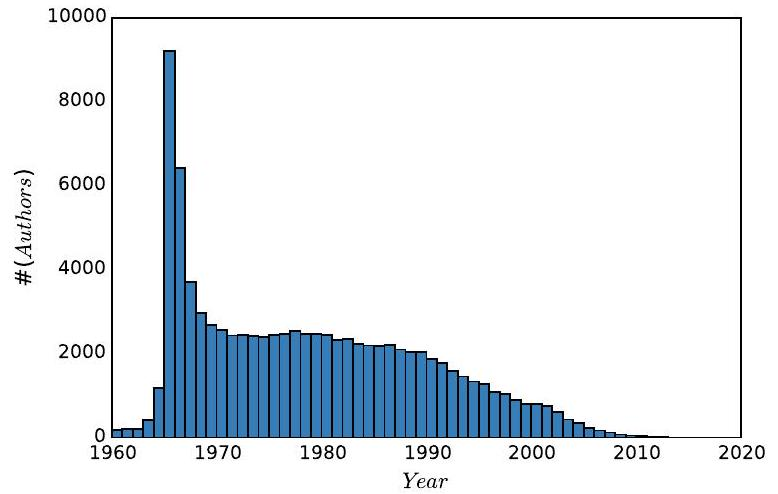
\includegraphics[max width=\textwidth]{2025_03_17_ca60ec0bfd96dcf8e028g-088}
  \caption{The cleaned data removes these artifacts, and the resulting distribution looks correct.}
\end{figure}

Figure \ref{fig:cleaned-data} shows our final distribution of authors, which matches the platonic ideal of what we expected the distribution to be. Don't be too quick to rationalize away how your data looks coming out of the computer. My collaborators were at one point ready to write off the 2002 bump as due to increases in research funding or the creation of new scientific journals. Always be suspicious of whether your data is clean enough to trust.

\subsubsection{Data Compatibility}
\index{compatibility}
We say that a comparison of two items is "apples to apples" when it is fair comparison, that the items involved are similar enough that they can be meaningfully stood up against each other. In contrast, "apples to oranges" comparisons are ultimately meaningless. For example:

\begin{itemize}
  \item It makes no sense to compare weights of 123.5 against 78.9, when one is in pounds and the other is in kilograms.
  \item It makes no sense to directly compare the movie gross of \emph{Gone with the Wind} against that of \emph{Avatar}, because 1939 dollars are 15.43 times more valuable than 2009 dollars.
  \item It makes no sense to compare the price of gold at noon today in New York and London, because the time zones are five hours off, and the prices are affected by intervening events.
  \item It makes no sense to compare the stock price of Microsoft on February 17, 2003 to that of February 18, 2003, because the intervening 2-for-1 stock split cut the price in half, but reflects no change in real value.
\end{itemize}

These types of data comparability issues arise whenever data sets are merged. Here I hope to show you how insidious such comparability issues can be, to sensitize you as to why you need to be aware of them. Further, for certain important classes of conversions, I point to ways to deal with them.

\emph{Take-Home Lesson:} Review the meaning of each of the fields in any data set you work with. If you do not understand what's in there down to the units of measurement, there is no sensible way you can use it.

\subsection{Unit Conversions}
Quantifying observations in physical systems requires standard units of measurement. Unfortunately, there exist many functionally equivalent but incompatible systems of measurement. My 12-year-old daughter and I both weigh about 70, but one of us is in pounds and the other in kilograms.

%---- Page End Break Here ---- Page : 72

Disastrous things like rocket explosions happen when measurements are entered into computer systems using the wrong units of measurement. In particular, NASA\index{NASA} lost the \$125 million Mars Climate Orbiter space mission on September 23, 1999 due to a metric-to-English conversion issue.

Such problems are best addressed by selecting a single system of measurements and sticking to it. The metric system offers several advantages over the traditional English system. In particular, individual measurements are naturally expressed as single decimal quantities (like 3.28 meters) instead of incomparable pairs of quantities (5 feet, 8 inches). This same issue arises in measuring angles (radians vs. degrees/seconds) and weight (kilograms vs. pounds/oz).

Sticking to the metric system does not by itself solve all comparability issues, since there is nothing to prevent you from mixing heights in meters and centimeters. But it is a good start.

How can you defend yourself against incompatible units when merging data sets? Vigilance has to be your main weapon. Make sure that you know the intended units for each numerical column in your data set, and verify compatibility when merging. Any column which does not have an associated unit or object type should immediately be suspect.

When merging records from diverse sources, it is an excellent practice to create a new "origin" or "source" field to identify where each record came from. This provides at least the hope that unit conversion mistakes can be corrected later, by systematically operating on the records from the problematic source.

A partially-automated procedure to detect such problems can be devised from statistical significance testing, to be discussed in Section 5.3. Suppose we were to plot the frequencies of human heights in a merged data set of English (feet) and metric (meter) measurements. We would see one peak in the distribution around 1.8 and a second around 5.5. The existence of multiple peaks in a distribution should make us suspicious. The \emph{p}-value resulting from significance testing on the two input populations provides a rigorous measurement of the degree to which our suspicions are validated.

\subsection{Numerical Representation Conversions}
Numerical features are the easiest to incorporate into mathematical models. Indeed, certain machine learning algorithms such as linear regression and support vector machines work only with numerically-coded data. But even turning numbers into numbers can be a subtle problem. Numerical fields might be represented in different ways: as integers (123), as decimals (123.5), or even as fractions (123 1/2). Numbers can even be represented as text, requiring the conversion from "ten million" to 10000000 for numerical processing.

Numerical representation issues can take credit for destroying another rocket ship. An Ariane 5 rocket launched at a cost of \$500 million on June 4, 1996 exploded forty seconds after lift-off, with the cause ultimately ascribed to an unsuccessful conversion of a 64-bit floating point number to a 16-bit integer.

The distinction between integers and floating point (real) numbers is important to maintain. Integers are counting numbers: quantities which are really discrete should be represented as integers. Physically measured quantities are never precisely quantified, because we live in a continuous world. Thus, all measurements should be reported as real numbers. Integer approximations of real numbers are sometimes used in a misbegotten attempt to save space. Don't do this: the quantification effects of rounding or truncation introduce artifacts.

In one particularly clumsy data set we encountered, baby weights were represented as two integer fields (pounds and the remaining ounces). Much better would have been to combine them into a single decimal quantity.

\subsection{Name Unification}
Integrating records from two distinct data sets requires them to share a common key field. Names are frequently used as key fields, but they are often reported inconsistently. Is \emph{José} the same fellow as \emph{Jose}? Such diacritic marks are banned from the official birth records of several U.S. states, in an aggressive attempt to force them to be consistent.

As another case in point, databases show my publications as authored by the Cartesian product of my first (\emph{Steve}, \emph{Steven}, or \emph{S.}), middle (\emph{Sol}, \emph{S.}, or blank), and last (\emph{Skiena}) names, allowing for nine different variations. And things get worse if we include misspellings. I can find myself on Google with a first name of \emph{Stephen} and last names of \emph{Skienna} and \emph{Skeina}.

Unifying records by key is a very ugly problem, which doesn't have a magic bullet. This is exactly why ID numbers were invented, so use them as keys if you possibly can.

The best general technique is unification: doing simple text transformations to reduce each name to a single canonical version. Converting all strings to lower case increases the number of (usually correct) collisions. Eliminating middle names or at least reducing them to an abbreviation creates even more name matches/collisions, as does mapping first names to canonical versions (like turning all \emph{Steves} into \emph{Stevens}).

Any such transformation runs the risk of creating Frankenstein-people, single records assembled from multiple bodies. Applications differ in whether the greater danger lies in merging too aggressively or too timidly. Figure out where your task sits on this spectrum and act accordingly.

An important concern in merging data sets is \emph{character code unification}. Characters in text strings are assigned numerical representations, with the mapping between symbols and numbers governed by the character code standard. Unfortunately, there are several different character code standards in common usage, meaning that what you scrape from a webpage might not be in the same character code as assumed by the system which will process it.

Historically, the good old 7-bit \emph{ASCII} code standard was expanded to the 8-bit \emph{ISO 8859-1 Latin} alphabet code, which adds characters and punctuation marks from several European languages. \emph{UTF-8} is an encoding of all Unicode characters using variable numbers of 8-bit blocks, which is backwards compatible with ASCII. It is the dominant encoding for web-pages, although other systems remain in use.

Correctly unifying character codes after merging is pretty much impossible. You must have the discipline to pick a single code as a standard, and check the encoding of each input file on preprocessing, converting it to the target before further work.

\subsection{Time/Date Unification}
Data/time stamps are used to infer the relative order of events, and group events by relative simultaneity. Integrating event data from multiple sources requires careful cleaning to ensure meaningful results.

First, let us consider issues in measuring time. The clocks from two computers never exactly agree, so precisely aligning logs from different systems requires a mix of work and guesswork. There are also time zone issues when dealing with data from different regions, as well as diversities in local rules governing changes in daylight saving time.

The right answer here is to align all time measurements to \emph{Coordinated Universal Time} (UTC), a modern standard subsuming the traditional \emph{Greenwich Mean Time} (GMT). A related standard is \emph{UNIX time}, which reports an event's precise time in terms of the number of elapsed seconds since 00:00:00 UTC on Thursday, January 1, 1970.

The Gregorian calendar is common throughout the technology world, although many other calendar systems are in use in different countries. Subtle algorithms must be used to convert between calendar systems. A bigger problem for date alignment concerns the proper interpretation of time zones and the international date line.

Time series unification is often complicated by the nature of the business calendar. Financial markets are closed on weekends and holidays, making for questions of interpretation when you are correlating, say, stock prices to local temperature. What is the right moment over the weekend to measure temperature, so as to be consistent with other days of the week? Languages like Python contain extensive libraries to deal with financial time series data to get issues like this correct. Similar issues arise with monthly data, because months (and even years) have different lengths.

\subsection{Financial Unification}
Money makes the world go round, which is why so many data science projects revolve around financial time series. But money can be dirty, so this data requires cleaning.

One issue here is \emph{currency conversion}, representing international prices using a standardized financial unit. Currency exchange rates can vary by a few percent within a given day, so certain applications require time-sensitive conversions. Conversion rates are not truly standardized. Different markets will each have different rates and \emph{spreads}, the gap between buying and selling prices that cover the cost of conversion.

The other important correction is for inflation. The \emph{time value of money} implies that a dollar today is (generally) more valuable than a dollar a year from now, with interest rates providing the right way to discount future dollars. Inflation rates are estimated by tracking price changes over baskets of items, and provide a way to standardize the purchasing power of a dollar over time.

Using unadjusted prices in a model over non-trivial periods of time is just begging for trouble. A group of my students once got very excited by the strong correlation observed between stock prices and oil prices over a thirty-year period, and so tried to use stock prices in a commodity prediction model. But both goods were priced in dollars, without any adjustment as they inflated. The time series of prices of essentially \emph{any} pair of items will correlate strongly over time when you do not correct for inflation.

In fact, the most meaningful way to represent price changes over time is probably not differences but \emph{returns}, which normalize the difference by the initial price:

\begin{equation}
r_{i} = \frac{p_{i+1}-p_{i}}{p_{i}}
\end{equation}

This is more analogous to a percentage change, with the advantage here that taking the logarithm of this ratio becomes symmetric to gains and losses.

Financial time series contain many other subtleties which require cleaning. Many stocks give scheduled \emph{dividends} to the shareholder on a particular date every year. Say, for example, that Microsoft will pay a \$2.50 dividend on January 16. If you own a share of Microsoft at the start of business that day, you receive this check, so the value of the share then immediately drops by \$2.50 the moment after the dividend is issued. This price decline reflects no real loss to the shareholder, but properly cleaned data needs to factor the dividend into the price of the stock. It is easy to imagine a model trained on uncorrected price data learning to sell stocks just prior to its issuing dividends, and feeling unjustly proud of itself for doing so.

\subsection{Dealing with Missing Values}
Not all data sets are complete. An important aspect of data cleaning is identifying fields for which data isn't there, and then properly compensating for them:

\begin{itemize}
  \item What is the year of death of a living person?
  \item What should you do with a survey question left blank, or filled with an obviously outlandish value?
  \item What is the relative frequency of events too rare to see in a limited-size sample?
\end{itemize}

Numerical data sets expect a value for every element in a matrix. Setting missing values to zero is tempting, but generally wrong, because there is always some ambiguity as to whether these values should be interpreted as data or not. Is someone's salary zero because he is unemployed, or did he just not answer the question?

The danger with using nonsense values as not-data symbols is that they can get misinterpreted as data when it comes time to build models. A linear regression model trained to predict salaries from age, education, and gender will have trouble with people who refused to answer the question.

Using a value like -1 as a no-data symbol has exactly the same deficiencies as zero. Indeed, be like the mathematician who is afraid of negative numbers: stop at nothing to avoid them.

\emph{Take-Home Lesson:} Separately maintain both the raw data and its cleaned version. The raw data is the ground truth, and must be preserved intact for future analysis. The cleaned data may be improved using imputation to fill in missing values. But keep raw data distinct from cleaned, so we can investigate different approaches to guessing.

So how should we deal with missing values? The simplest approach is to drop all records containing missing values. This works just fine when it leaves enough training data, provided the missing values are absent for non-systematic reasons. If the people refusing to state their salary were generally those above the mean, dropping these records will lead to biased results.

But typically we want to make use of records with missing fields. It can be better to estimate or \emph{impute} missing values, instead of leaving them blank. We need general methods for filling in missing values. Candidates include:

\begin{itemize}
  \item \emph{Heuristic-based imputation:} Given sufficient knowledge of the underlying domain, we should be able to make a reasonable guess for the value of certain fields. If I need to fill in a value for the year you will die, guessing \emph{birth year +80} will prove about right on average, and a lot faster than waiting for the final answer.
  \item \emph{Mean value imputation:} Using the mean value of a variable as a proxy for missing values is generally sensible. First, adding more values with the mean leaves the mean unchanged, so we do not bias our statistics by such imputation. Second, fields with mean values add a vanilla flavor to most models, so they have a muted impact on any forecast made using the data.
\end{itemize}

But the mean might not be appropriate if there is a systematic reason for missing data. Suppose we used the mean death-year in Wikipedia to impute the missing value for all living people. This would prove disastrous, with many people recorded as dying before they were actually born.

\begin{itemize}
  \item \emph{Random value imputation:} Another approach is to select a random value from the column to replace the missing value. This would seem to set us up for potentially lousy guesses, but that is actually the point. Repeatedly selecting random values permits statistical evaluation of the impact of imputation. If we run the model ten times with ten different imputed values and get widely varying results, then we probably shouldn't have much confidence in the model. This accuracy check is particularly valuable when there is a substantial fraction of values missing from the data set.
  \item \emph{Imputation by nearest neighbor:} What if we identify the complete record which matches most closely on all fields present, and use this nearest neighbor to infer the values of what is missing? Such predictions should be more accurate than the mean, when there are systematic reasons to explain variance among records.
\end{itemize}

This approach requires a distance function to identify the most similar records. \emph{Nearest neighbor} methods are an important technique in data science, and will be presented in greater detail in Section 10.2.

\begin{itemize}
  \item \emph{Imputation by interpolation:} More generally, we can use a method like linear regression (see Section 9.1) to predict the values of the target column, given the other fields in the record. Such models can be trained over full records and then applied to those with missing values.
\end{itemize}

Using linear regression to predict missing values works best when there is only one field missing per record. The potential danger here is creating significant outliers through lousy predictions. Regression models can easily turn an incomplete record into an outlier, by filling the missing fields in with unusually high or low values. This would lead downstream analysis to focus more attention on the records with missing values, exactly the opposite of what we want to do.

Such concerns emphasize the importance of outlier detection, the final step in the cleaning process that will be considered here.

\subsubsection{Outlier Detection}
Mistakes in data collection can easily produce outliers that can interfere with proper analysis. An interesting example concerns the largest dinosaur vertebra\index{dinosaur vertebra} ever discovered. Measured at 1500 millimeters, it implies an individual that was 188 feet long. This is amazing, particularly because the \emph{second} largest specimen ever discovered comes in at only 122 feet.

The most likely explanation here (see [\cite{goldenberg2016biggest}]) is that this giant fossil never actually existed: it has been missing from the American Museum of Natural History for over a hundred years. Perhaps the original measurement was taken on a conventionally-sized bone and the center two digits accidentally transposed, reducing the vertebra down to 1050 millimeters.

Outlier elements are often created by data entry mistakes, as apparently was the case here. They can also result from errors in scraping, say an irregularity in formatting causing a footnote number to be interpreted as a numerical value. Just because something is written down doesn't make it correct. As with the dinosaur example, a single outlier element can lead to major misinterpretations.
%---- Page End Break Here ---- Page : 78
```latex
\section{General sanity checking and outlier detection}

General sanity checking requires looking at the largest and smallest values in each variable/column to see whether they are too far out of line. This can best be done by plotting the frequency histogram and looking at the location of the extreme elements. Visual inspection can also confirm that the distribution looks the way it should, typically bell-shaped.

In normally distributed data, the probability that a value is $k$ standard deviations from the mean decreases exponentially with $k$. This explains why there are no 10-foot basketball players, and provides a sound threshold to identify outliers. Power law distributions are less easy to detect outliers in: there really \textit{is} a Bill Gates worth over 10,000 times as much as the average individual.

It is too simple to just delete the rows containing outlier fields and move on. Outliers often point to more systematic problems that one must deal with. Consider a data set of historical figures by lifespan. It is easy to finger the biblical Methuselah (at 969 years) as an outlier, and remove him.

But it is better to figure out whether he is indicative of other figures that we should consider removing. Observe that Methuselah had no firmly established birth and death dates. Perhaps the published ages of anybody without dates should be considered suspicious enough to prune. By contrast, the person with the shortest lifespan in \index{Wikipedia}Wikipedia (John I, King of France) lived only five days. But his birth (November 15) and death (November 20) dates in 1316 convinces me that his lifespan was accurate.

\subsection{War Story: Beating the Market}

Every time we met, my graduate student Wenbin told me we were making money. But he sounded less and less confident every time I asked.

Our Lydia sentiment analysis system took in massive text feeds of news and social media, reducing them to daily time series of frequency and sentiment for the millions of different people, places, and organizations mentioned within. When somebody wins a sports championship, many articles get written describing how great an athlete they are. But when this player then gets busted on drug charges, the tone of the articles about them immediately changes. By keeping count of the relative frequency of association with positive words ("victorious") vs. negative words ("arrested") in the text stream, we can construct sentiment signals for any news-worthy entity.

Wenbin studied how sentiment signals could be used to predict future events like the gross for a given movie, in response to the quality of published reviews or buzz. But he particularly wanted to use this data to play the stock market\index{stock market}. Stocks move up and down according to news. A missed earnings report is bad news for a company, so the price goes down. Food and Drug Administration (FDA) approval of a new drug is \textit{great} news for the company which owns it, so the price goes up. If Wenbin could use our sentiment signal to predict future stock prices, well, let's just say I wouldn't have to pay him as a research assistant anymore.

So he simulated a strategy of buying the stocks that showed the highest sentiment in that day's news, and then shorting those with the lowest sentiment. He got great results. "See," he said. "We are making money."

The numbers looked great, but I had one quibble. Using today's news results to predict current price movements wasn't really fair, because the event described in the article may have already moved the price before we had any chance to read about it. Stock prices should react very quickly to important news.

So Wenbin simulated the strategy of buying stocks based on sentiment from the previous day's news, to create a gap between the observed news and price changes. The return rate went down substantially, but was still positive. "See," he said. "We are still making money."

But I remained a little uncomfortable with this. Many economists believe that the financial markets are \textit{efficient}, meaning that all public news is instantly reflected in changing prices. Prices certainly changed in response to news, but you would not be able to get in fast enough to exploit the information. We had to remain skeptical enough to make sure there were no data/timing problems that could explain our results.

So I pressed Wenbin about exactly how he had performed his simulation. His strategy bought and sold at the closing price every day. But that left sixteen hours until the next day's open, plenty of time for the world to react to events that happened while I slept. He switched his simulated purchase to the opening price. Again, the return rate went down substantially, but was still positive. "See," he said. "We are still making some money."

But might there still be other artifacts in how we timed our data, giving us essentially tomorrow's newspaper today? In good faith, we chased down all other possibilities we could think of, such as whether the published article dates reflected when they appeared instead of when they were written. After doing our best to be skeptical, his strategies still seemed to show positive returns from news sentiment.

Our paper on this analysis \cite{\cite{zhang2010trading}} has been well received, and Wenbin has gone on to be a successful quant, using sentiment among other signals to trade in the financial markets. But I remain slightly queasy about this result. Cleaning our data to precisely time-stamp each news article was very difficult to do correctly. Our system was originally designed to produce daily time series in a batch mode, so it is hard to be sure that we did everything right in the millions of articles downloaded over several years to now perform finer-scale analysis.

The take-home lesson is that cleanliness is important when there is money on the line. Further, it is better to design a clean environment at the beginning of analysis instead of furiously washing up at the end.

\subsection{Crowdsourcing}

No single person has all the answers. Not even me. Much of what passes for wisdom is how we aggregate expertise, assembling opinions from the knowledge and experience of others.

\begin{figure}[h]
  \centering
  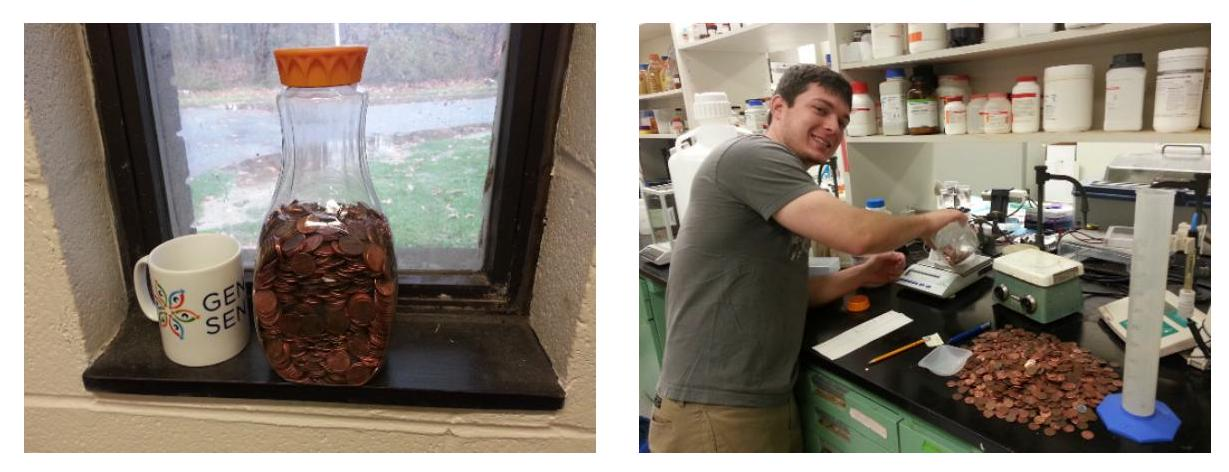
\includegraphics[max width=\textwidth]{2025_03_17_ca60ec0bfd96dcf8e028g-098}
  \caption{Guess how many pennies I have in this jar? (left) The correct answer was determined using precise scientific methods (right).}
  \label{fig:penny_jar}
\end{figure}

\textit{Crowdsourcing} harnesses the insights and labor from large numbers of people towards a common goal. It exploits the \textit{wisdom of crowds}, that the collective knowledge of a group of people might well be greater than that of the smartest individual among them.

This notion began with an ox. Francis Galton, a founder of statistical science and a relative of Charles Darwin, attended a local livestock fair in 1906. As part of the festivities, villagers were invited to guess the weight of this particular ox, with the person whose guess proved closest to the mark earning a prize. Almost 800 participants took a whack at it. No one picked the actual weight of 1,178 pounds, yet Galton observed that the average guess was amazingly close: 1,179 pounds! Galton's experiment suggests that for certain tasks one can get better results by involving a diverse collection of people, instead of just asking the experts.

Crowdsourcing serves as an important source of data in building models, especially for tasks associated with human perception. Humans remain the state-of-the-art system in natural language processing and computer vision, achieving the highest level of performance. The best way to gather training data often requires asking people to score a particular text or image. Doing this on a large enough scale to build substantial training data typically requires a large number of annotators, indeed a crowd.

Social media and other new technologies have made it easier to collect and aggregate opinions on a massive scale. But how can we separate the wisdom of crowds from the cries of the rabble?

\subsection{The Penny Demo}

Let's start by performing a little wisdom of crowds experiment of our own. Figure~\ref{fig:penny_jar} contains photos of a jar of pennies I accumulated in my office over many years. How many pennies do I have in this jar? Make your own guess now, because I am going to tell you the answer on the next page.

To get the right answer, I had my biologist-collaborator Justin Garden weigh the pennies on a precision laboratory scale. Dividing by the weight of a single penny gives the count. Justin can be seen diligently performing his task in Figure~\ref{fig:penny_jar} (right).

So I ask again: how many pennies do you think I have in this jar? I performed this experiment on students in my data science class. How will your answer compare to theirs?

I first asked eleven of my students to write their opinions on cards and quietly pass them up to me at the front of the room. Thus these guesses were completely independent of each other. The results, sorted for convenience, were:

$$
537, \, 556, \, 600, \, 636, \, 1200, \, 1250, \, 2350, \, 3000, \, 5000, \, 11{,}000, \, 15{,}000.
$$

I then wrote these numbers on the board, and computed some statistics. The median of these guesses was 1250, with a mean of 3739. In fact, there were exactly 1879 pennies in the jar. The median score among my students was closer to the right amount than any single guess.

But before revealing the actual total, I then asked another dozen students to guess. The only difference was that this cohort had seen the guesses from the first set of students written on the board. Their choices were:
$$
750, \, 750, \, 1000, \, 1000, \, 1000, \, 1250, \, 1400, \, 1770, \, 1800, \, 3500, \, 4000, \, 5000.
$$
Exposing the cohort to other people's guesses strongly conditioned the distribution by eliminating all outliers: the minimum among the second group was greater than four of the previous guesses, and the maximum less than or equal to three of the previous round. Within this cohort, the median was 1325 and the mean 1935. Both happen to be somewhat closer to the actual answer, but it is clear that group-think had settled in to make it happen.

\textit{Anchoring} is the well-known cognitive bias that people's judgments get irrationally fixated on the first number they hear. Car dealers exploit this all the time, initially giving an inflated cost for the vehicle so that subsequent prices sound like a bargain.

I then did one final test before revealing the answer. I allowed my students to bid on the jar, meaning that they had to be confident enough to risk money on the result. This yielded exactly two bids from brave students, at 1500 and 2000 pennies respectively. I pocketed \$1.21 from the sucker with the high bid, but both proved quite close. This is not a surprise: people willing to bet their own money on an event are, by definition, confident in their selection.

\subsection{When is the Crowd Wise?}

According to James Surowiecki in his book \textit{The Wisdom of Crowds} \cite{\cite{surowiecki2005wisdom}}, crowds are wise when four conditions are satisfied:

\begin{itemize}
    \item \textit{When the opinions are independent:} Our experiment highlighted how easy it is for a group to lapse into group-think. People naturally get influenced by others. If you want someone's true opinion, you must ask them in isolation.
    \item \textit{When crowds are people with diverse knowledge and methods:} Crowds only add information when there is disagreement. A committee composed of perfectly-correlated experts contributes nothing more than you could learn from any one of them. In the penny-guessing problem, some people estimated the volume of the container, while others gauged the sag of my arm as I lifted the heavy mass. Alternate approaches might have estimated how many pennies I could have accumulated in twenty years of occasionally emptying my pockets, or recalled their own hoarding experiences.
    \item \textit{When the problem is in a domain that does not need specialized knowledge:} I trust the consensus of the crowd in certain important decisions, like which type of car to buy or who should serve as the president of my country (gulp). But when it comes to deciding whether my tumor sample is cancerous or benign, I will trust the word of one doctor over a cast of 1,000 names drawn at random from the phonebook.\\
    Why? Because the question at hand benefits greatly from specialized knowledge and experience. There is a genuine reason why the doctor \textit{should} know more than all the others. For simpler perceptual tasks the mob rules, but one must be careful not to ask the crowd something they have no way of knowing.
    \item \textit{Opinions can be fairly aggregated:} The least useful part of any mass survey form is the open response field "Tell us what you think!". The problem here is that there is no way to combine these opinions to form a consensus, because different people have different issues and concerns. Perhaps these texts could be put into buckets by similarity, but this is hard to do effectively.\\
    The most common use of such free-form responses are anecdotal. People cherry-pick the most positive-sounding ones, then put them on a slide to impress the boss.
\end{itemize}

\textit{Take-Home Lesson:} Be an incomparable element on the partial order of life. Diverse, independent thinking contributes the most wisdom to the crowd.

\subsection{Mechanisms for Aggregation}

Collecting wisdom from a set of responses requires using the right aggregation mechanism. For estimating numerical quantities, standard techniques like plotting the frequency distribution and computing summary statistics are appropriate. Both the mean and median implicitly assume that the errors are symmetrically distributed. A quick look at the shape of the distribution can generally confirm or reject that hypothesis.

The median is, generally speaking, a more appropriate choice than the mean in such aggregation problems. It reduces the influence of outliers, which is a particular problem in the case of mass experiments where a certain fraction of your participants are likely to be bozos. On our penny guessing data, the mean produced a ghastly over-estimate of 3739, which reduced to 2843 after removing the largest and smallest guess, and then down to 2005 once trimming the two outliers on each end (recall the correct answer was 1879).

Removing outliers is a very good strategy, but we may have other grounds to judge the reliability of our subjects, such as their performance on other tests where we do know the answer. Taking a \textit{weighted average}, where we give more weight to the scores deemed more reliable, provides a way to take such confidence measures into account.

For classification problems, voting is the basic aggregation mechanism. The \textit{Condorcet jury theorem} justifies our faith in democracy. It states that if the probability of each voter being correct on a given issue is $p>0.5$, the probability that a majority of the voters are correct ($P(n)$) is greater than $p$. In fact, it is exactly:

$$
P(n) = \sum_{i=(n+1)/2}^{n}\binom{n}{i} p^{i}(1-p)^{n-i}
$$

Large voter counts give statistical validity even to highly contested elections. Suppose $p=0.51$, meaning the forces of right are a bare majority. A jury of 101 members would reach the correct decision $57\%$ of the time, while $P(1001)=0.73$ and $P(10001)=0.9999$. The probability of a correct decision approaches 1 as $n \rightarrow \infty$.

There are natural limitations to the power of electoral systems, however. \textit{Arrow's impossibility theorem} states that no electoral system for summing permutations of preferences as votes satisfies four natural conditions for the fairness of an election. This will be discussed in Section 4.6, in the context of scores and rankings.

\subsection{Crowdsourcing Services}

Crowdsourcing services like Amazon Turk\index{Amazon Turk} and CrowdFlower\index{CrowdFlower} provide the opportunity for you to hire large numbers of people to do small amounts of piecework. They help you to wrangle people, in order to create data for you to wrangle.

These crowdsourcing services maintain a large stable of freelance workers, serving as the middleman between them and potential employers. These workers, generally called \textit{Turkers}, are provided with lists of available jobs and what they will pay, as shown in Figure 3.5. Employers generally have some ability to control the location and credentials of who they hire, and the power to reject a worker's efforts without pay, if they deem it inadequate. But statistics on employers' acceptance rates are published, and good workers are unlikely to labor for bad actors.

\begin{figure}[h]
  \centering
  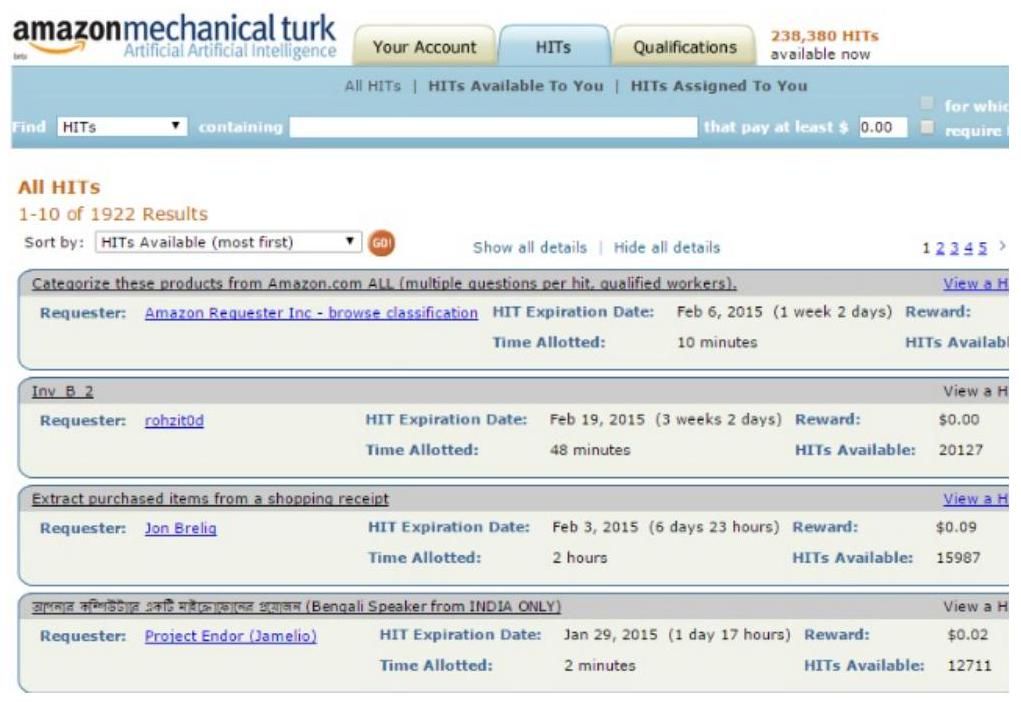
\includegraphics[max width=\textwidth]{2025_03_17_ca60ec0bfd96dcf8e028g-102}
  \caption{Representative tasks on Mechanical Turk.}
  \label{fig:tasks_mechanical_turk}
\end{figure}

The tasks assigned to Turkers generally involve simple cognitive efforts that cannot currently be performed well by computers. Good applications of Turkers include:

\begin{itemize}
    \item \textit{Measuring aspects of human perception:} Crowdsourcing systems provide efficient ways to gather representative opinions on simple tasks. One nice application was establishing linkages between colors in red-green-blue space, and the names by which people typically identify them in a language. This is important to know when writing descriptions of products and images.\\
          So where is the boundary in color space between "blue" and "light blue," or "robin’s egg blue" and "teal"? The right names are a function of culture and convention, not physics. To find out, you must ask people, and crowdsourcing permits you to easily query hundreds or thousands of different people.
    \item \textit{Obtaining training data for machine learning classifiers:} Our primary interest in crowdsourcing will be to produce human annotations that serve as training data. Many machine learning problems seek to do a particular task "as well as people do." Doing so requires a large number of training instances to establish what people did, when given the chance.\\
          For example, suppose we sought to build a sentiment analysis system capable of reading a written review and deciding whether its opinion of a product is favorable or unfavorable. We will need a large number of reviews labeled by annotators to serve as testing/training data. Further, we need the same reviews labeled repeatedly by different annotators, so as to identify any inter-annotator disagreements concerning the exact meaning of a text.
    \item \textit{Obtaining evaluation data for computer systems:} A/B testing is a standard method for optimizing user interfaces: show half of the judges version $A$ of a given system and the other half version $B$. Then test which group did better according to some metric. Turkers can provide feedback on how interesting a given app is, or how well a new classifier is performing.\\
          One of my grad students (Yanqing Chen) used CrowdFlower\index{CrowdFlower} to evaluate a system he built to identify the most relevant Wikipedia category for a particular entity. Which category better describes Barack Obama: \textit{Presidents of the United States} or \textit{African-American Authors}? For \$200, he got people to answer a total of 10,000 such multiple-choice questions, enough for him to properly evaluate his system.
    \item \textit{Putting humans into the machine:} There still exist many cognitive tasks that people do much better than machines. A cleverly-designed interface can supply user queries to people sitting inside the computer, waiting to serve those in need.\\
          Suppose you wanted to build an app to help the visually impaired, enabling the user to snap a picture and ask someone for help. Maybe they are in their kitchen, and need someone to read the label on a can to them. This app could call a Turker as a subroutine, to do such a task as it is needed.\\
          Of course, these image-annotation pairs should be retained for future analysis. They could serve as training data for a machine learning program to take the people out of the loop, as much as possible.
    \item \textit{Independent creative efforts:} Crowdsourcing can be used to commission large numbers of creative works on demand. You can order blog posts or articles on demand, or written product reviews both good and bad. Anything that you might imagine can be created, if you just specify what you want.\\
          Here are two silly examples that I somehow find inspiring:
          \begin{itemize}
              \item \textbf{The Sheep Market} (\url{http://www.thesheepmarket.com}) commissioned 10,000 drawings of sheep for pennies each. As a conceptual art piece, it tries to sell them to the highest bidder. What creative endeavors can you think of that people will do for you at \$0.25 a pop?
              \item \textbf{Emoji Dick} (\url{http://www.emojidick.com}) was a crowdsourced effort to translate the great American novel \textit{Moby Dick} completely into emoji images. Its creators partitioned the book into roughly 10,000 parts, and farmed out each part to be translated by three separate Turkers. Other Turkers were hired to select the best one of these to be incorporated into the final book. Over 800 Turkers were involved, with the total cost of \$3,676 raised by the crowd-funding site Kickstarter.
          \end{itemize}
    \item \textit{Economic/psychological experiments:} Crowdsourcing has proven a boon to social scientists conducting experiments in behavioral economics and psychology. Instead of bribing local undergraduates to participate in their studies, these investigators can now expand their subject pool to the entire world. They get the power to harness larger populations, perform independent replications in different countries, and thus test whether there are cultural biases in their hypotheses.
\end{itemize}

There are many exciting tasks that can be profitably completed using crowdsourcing. However, you are doomed to disappointment if you employ Turkers for the wrong task, in the wrong way. Bad uses of crowdsourcing include:

\begin{itemize}
    \item \textit{Any task that requires advanced training:} Although every person possesses unique skills and expertise, crowdsourcing workers come with no specific training. They are designed to be treated as interchangeable parts. You do not establish a personal relationship with these workers, and any sensible gig will be too short to allow for more than a few minutes training.\\
          Tasks requiring specific technical skills are not reasonably crowdsourced. However, they might be reasonably subcontracted, in traditional longer-term arrangements.
    \item \textit{Any task you cannot specify clearly:} You have no mechanism for back-and-forth communication with Turkers. Generally speaking, they have no way to ask you questions. Thus the system works only if you can specify your tasks clearly, concisely, and unambiguously.\\
          This is much harder than it looks. Realize that you are trying to program people instead of computers, with all the attendant bugs associated with "do as I say" trumping "do what I mean." Test your specifications out on local people before opening up your job to the masses, and then do a small test run on your crowdsourcing platform to evaluate how it goes before cutting loose with the bulk of your budget. You may be in for some cultural surprises. Things that seem obvious to you might mean something quite different to a worker halfway around the world.
    \item \textit{Any task where you cannot verify whether they are doing a good job:} Turkers have a single motivation for taking on your piecework: they are trying to convert their time into money as efficiently as possible. They are looking out for jobs offering the best buck for their bang, and the smartest ones will seek to complete your task as quickly and thoughtlessly as possible.\\
          Crowdsourcing platforms permit employers to withhold payment if the contracted work is unacceptable. Taking advantage of this requires some efficient way to check the quality of the product. Perhaps you should ask them to complete certain tasks where you already know the correct answer. Perhaps you can compare their responses to that of other independent workers, and throw out their work if it disagrees too often from the consensus.
    \item \textit{Any illegal task, or one too inhuman to subject people to:} You are not allowed to ask a Turker to do something illegal or unethical. The classic example is hiring someone to write bad reviews of your competitor's products. Hiring a hit man makes you just as guilty of murder as the guy who fired the shots. Be aware that there are electronic trails that can be followed from the public placement of your ad directly back to you.\\
          People at educational and research institutions are held to a higher standard than the law, through their \textit{institutional review board} or IRB. The IRB is a committee of researchers and administrative officials who must approve any research on human subjects before it is undertaken. Benign crowdsourcing applications such as the ones we have discussed are routinely approved, after the researchers have undergone a short online training course to make sure they understand the rules.\\
          Always realize that there is a person at the other end of the machine. Don’t assign them tasks that are offensive, degrading, privacy-violating, or too stressful. You will probably get better results out of your workers if you treat them like human beings.
\end{itemize}

Getting people to do your bidding requires proper incentives, not just clear instructions. In life, you generally get what you pay for. Be aware of the currently prevailing minimum hourly wage in your country, and price your tasks accordingly. This is not a legal requirement, but it is generally good business.

The sinister glow that comes from hiring workers at \$0.50 per hour wears off quickly once you see the low quality of workers that your tasks attract. You can easily eat up all your savings by the need to rigorously correct their work product, perhaps by paying multiple workers do it repeatedly. Higher paying tasks find workers much more quickly, so be prepared to wait if you do not pay the prevailing rate. Bots and their functional equivalents are happier to accept slave wages than the workers you really want to hire.

\subsection{Gamification}

There is an alternative to paying people to annotate or transcribe your data. Instead, make things so much fun that people will work for you for free!

\textit{Games with a purpose} (GWAP) are systems which disguise data collection as a game people want to play, or a task people themselves want done. With the right combination of game, motive, and imagination, amazing things can be done. Successful examples include:

\begin{itemize}
    \item \textit{CAPTCHAs for optical character recognition (OCR):} CAPTCHAs are those distorted text images you frequently encounter when creating an account on the web. They demand that you type in the contents of text strings shown in the image to prove that you are a human, thus enabling them to deny access to bots and other programmed systems.\\
          ReCAPTCHAs were invented to get useful data from the over 100 million CAPTCHAs displayed each day. Two text strings are displayed in each, one of which the system checks in order to grant entry. The other represents a hard case for an OCR system that is digitizing old books and newspapers. The answers are mapped back to improve the digitization of archival documents, transcribing over 40 million words per day.
    \item \textit{Psychological/IQ testing in games/apps:} Psychologists have established five basic personality traits as important and reproducible aspects of personality. Academic psychologists use multiple-choice personality tests to measure where individuals sit along personality scales for each of the big five traits: openness, conscientiousness, extroversion, agreeableness, and neuroticism.\\
          By turning these surveys into game apps ("What are \textit{your} personality traits?") psychologists have gathered personality measurements on over 75,000 different people, along with other data on preferences and behavior. This has created an enormous data set to study many interesting issues in the psychology of personality.
    \item \textit{The FoldIt game for predicting protein structures:} Predicting the structures formed by protein molecules is one of the great computational challenges in science. Despite many years of work, what makes a protein fold into a particular shape is still not well understood.\\
          FoldIt (\url{https://fold.it}) is a game challenging non-biologists to design protein molecules that fold into a particular shape. Players are scored as to how closely their design approaches the given target, with the highest scoring players ranked on a leader board. Several scientific papers have been published on the strength of the winning designs.
\end{itemize}

The key to success here is making a game that is playable enough to become popular. This is much harder than it may appear. There are millions of free apps in the app store, mostly games. Very few are ever tried by more than a few hundred people, which is nowhere near enough to be interesting from a data collection standpoint. Adding the extra constraint that the game generates interesting scientific data while being playable makes this task even harder.

Motivational techniques should be used to improve playability. Keeping score is an important part of any game, and the game should be designed so that performance increases rapidly at first, in order to hook the player. Progress bars...
```
%---- Page End Break Here ---- Page : 89
```latex
\subsection*{3.6 Chapter Notes}
The Charles Babbage quote from the start of this chapter is from his book \textit{Passages from the Life of a Philosopher} \cite{\cite{babbage2011passages}}. I recommend Padua's graphic novel \cite{\cite{padua2015thrilling}} for an amusing but meaningful (albeit fictitious) introduction to his work and relationship with Ada Lovelace.

Many books deal with hands-on practical matters of data wrangling in particular programming languages. Particularly useful are the O'Reilly books for data science in Python, including \cite{\cite{grus2015data}}, \cite{\cite{mckinney2012python}}.

The story of our jai-alai betting system, including the role of website scraping, is reported in my book \textit{Calculated Bets} \cite{\cite{skiena2001calculated}}. It is a quick and fun overview of how to build simulation models for prediction, and will be the subject of the war story of Section 7.8.

The failure of space missions due to numerical computing errors has been well chronicled in popular media. See Gleick \cite{\cite{gleick1996bug}} and Stephenson et al. \cite{\cite{stephenson1999mars}} for discussions of the Ariane 5 and Mars Climate Orbiter space missions, respectively.

The clever idea of using accelerometers in cell phones to detect earthquakes comes from Faulkner et al. \cite{\cite{faulkner2014community}}. Representative studies of large sets of Flickr images includes Kisilevich et al. \cite{\cite{kisilevich2010event}}.

Kittur \cite{\cite{kittur2008crowdsourcing}} reports on experiences with crowdsourcing user studies on Amazon Turk. Our use of CrowdFlower to identify appropriate descriptions of historical figures was presented in \cite{\cite{chen2015vector}}. Methods for gamification in instruction are discussed in \cite{\cite{deterding2011game}, \cite{kapp2012gamification}}. Recaptchas are introduced in Von Ahn, et al. \cite{\cite{vonahn2008recaptcha}}. The large-scale collection of psychological trait data via mobile apps is due to Kosinski, et al. \cite{\cite{kosinski2013private}}.

\subsection*{3.7 Exercises}
\section*{Data Munging}
3-1. [3] Spend two hours getting familiar with one of the following programming languages: Python, R, MatLab, Wolfram Alpha/Language. Then write a brief paper with your impressions on its characteristics:
\begin{itemize}
  \item Expressibility.
  \item Runtime speed.
  \item Breadth of library functions.
  \item Programming environment.
  \item Suitability for algorithmically-intensive tasks.
  \item Suitability for general data munging tasks.
\end{itemize}

3-2. [5] Pick two of the primary data science programming languages, and write programs to solve the following tasks in both of them. Which language did you find most suitable for each task?\\
(a) Hello World!\\
(b) Read numbers from a file, and print them out in sorted order.\\
(c) Read a text file, and count the total number of words.\\
(d) Read a text file, and count the total number of \textit{distinct} words.\\
(e) Read a file of numbers, and plot a frequency histogram of them.\\
(f) Download a page from the web, and scrape it.

3-3. [3] Play around for a little while with Python, R, and Matlab. Which do you like best? What are the strengths and weaknesses of each?\\
3-4. [5] Construct a data set of \textit{n} human heights, with \textit{p}\% of them recorded in English (feet) and the rest with metric (meter) measurements. Use statistical tests to test whether this distribution is distinguishable from one properly recorded in meters. What is the boundary as a function of \textit{n} and \textit{p} where it becomes clear there is a problem?

\section*{Data Sources}
3-5. [3] Find a table of storage prices over time. Analyze this data, and make a projection about the cost/volume of data storage five years from now. What will disk prices be in 25 or 50 years?\\
3-6. [5] For one or more of the following \textit{The Quant Shop} challenges, find relevant data sources and assess their quality:
\begin{itemize}
  \item \textit{Miss Universe}.
  \item \textit{Movie gross}.
  \item \textit{Baby weight}.
  \item \textit{Art auction price}.
  \item \textit{Snow on Christmas}.
  \item \textit{Super Bowl/college champion}.
  \item \textit{Ghoul pool}.
  \item \textit{Future gold/oil price}.
\end{itemize}

\section*{Data Cleaning}
3-7. [3] Find out what was weird about September 1752. What special steps might the data scientists of the day have had to take to normalize annual statistics?\\
3-8. [3] What types of outliers might you expect to occur in the following data sets:\\
(a) Student grades.\\
(b) Salary data.\\
(c) Lifespans in Wikipedia.

3-9. [3] A health sensor produces a stream of twenty different values, including blood pressure, heart rate, and body temperature. Describe two or more techniques you could use to check whether the stream of data coming from the sensor is valid.

\section*{Implementation Projects}
3-10. [5] Implement a function that extracts the set of hashtags from a data frame of tweets. Hashtags begin with the "\#" character and contain any combination of upper and lowercase characters and digits. Assume the hashtag ends where there is a space or a punctuation mark, like a comma, semicolon, or period.

3-11. [5] The laws governing voter registration records differ from state to state in the United States. Identify one or more states with very lax rules, and see what you must do to get your hands on the data. Hint: Florida.

\section*{Crowdsourcing}
3-12. [5] Describe how crowdsourced workers might have been employed to help gather data for \textit{The Quant Shop} challenges:
\begin{itemize}
  \item \textit{Miss Universe}.
  \item \textit{Movie gross}.
  \item \textit{Baby weight}.
  \item \textit{Art auction price}.
  \item \textit{Snow on Christmas}.
  \item \textit{Super Bowl/college champion}.
  \item \textit{Ghoul pool}.
  \item \textit{Future gold/oil price}.
\end{itemize}

3-13. [3] Suppose you are paying Turkers to read texts and annotate them based on the underlying sentiment (positive or negative) that each passage conveys. This is an opinion task, but how can we algorithmically judge whether the Turker was answering in a random or arbitrary manner instead of doing their job seriously?

\section*{Interview Questions}
3-14. [5] Suppose you built a system to predict stock prices. How would you evaluate it?\\
3-15. [5] In general, how would you screen for outliers, and what should you do if you find one?

3-16. [3] Why does data cleaning play a vital role in analysis?\\
3-17. [5] During analysis, how do you treat missing values?\\
3-18. [5] Explain selection bias. Why is it important? How can data management procedures like handling missing data make it worse?\\
3-19. [3] How do you efficiently scrape web data?

\section*{Kaggle Challenges}
3-20. Partially sunny, with a chance of hashtags. \url{https://www.kaggle.com/c/crowdflower-weather-twitter}\\
3-21. Predict end of day stock returns, without being deceived by noise. \url{https://www.kaggle.com/c/the-winton-stock-market-challenge}\\
3-22. Data cleaning and the analysis of historical climate change. \url{https://www.kaggle.com/berkeleyearth/climate-change-earth-surface-temperature-data}

\section*{Chapter 4}
\section*{Scores and Rankings}
\begin{flushright}
Money is a scoreboard where you can rank how you're doing against other people. 
\\ — Mark Cuban
\end{flushright}

\textit{Scoring functions} are measures that reduce multi-dimensional records to a single value, highlighting some particular property of the data. A familiar example of scoring functions are those used to assign student grades in courses such as mine. Students can then be ranked (sorted) according to these numerical scores, and later assigned letter grades based on this order.

Grades are typically computed by functions over numerical features that reflect student performance, such as the points awarded on each homework and exam. Each student receives a single combined score, often scaled between 0 and 100. These scores typically come from a linear combination of the input variables, perhaps giving 8\% weight to each of five homework assignments, and 20\% weight to each of three exams.

There are several things to observe about such grading rubrics, which we will use as a model for more general scoring and ranking functions:

\begin{itemize}
  \item \textit{Degree of arbitrariness}: Every teacher/professor uses a different trade-off between homework scores and exams when judging their students. Some weigh the final exam more than all the other variables. Some normalize each value to 100 before averaging, while others convert each score to a Z-score. They all differ in philosophy, yet every teacher/professor is certain that their grading system is the best way to do things.
  \item \textit{Lack of validation data}: There is no gold standard informing instructors of the "right" grade that their students \textit{should} have received in the course. Students often complain that I should give them a better grade, but self-interest seems to lurk behind these requests more than objectivity. Indeed, I rarely hear students recommend that I lower their grade.
\end{itemize}

Without objective feedback or standards to compare against, there is no rigorous way for me to evaluate my grading system and improve it.

\begin{itemize}
  \item \textit{General Robustness}: And yet, despite using widely-disparate and totally unvalidated approaches, different grading systems generally produce similar results. Every school has a cohort of straight-A students who monopolize a sizable chunk of the top grades in each course. This couldn't happen if all these different grading systems were arbitrarily ordering student performance. C students generally muddle along in the middle-to-lower tiers of the bulk of their classes, instead of alternating As and Fs on the way to their final average. All grading systems are different, yet almost all are defensible.
\end{itemize}

In this chapter, we will use scoring and ranking functions as our first foray into data analysis. Not everybody loves them as much as I do. Scoring functions often seem arbitrary and ad hoc, and in the wrong hands can produce impressive-looking numbers which are essentially meaningless. Because their effectiveness generally cannot be validated, these techniques are not as scientifically sound as the statistical and machine learning methods we will present in subsequent chapters.

But I think it is important to appreciate scoring functions for what they are: useful, heuristic ways to tease understanding from large data sets. A scoring function is sometimes called a \textit{statistic}, which lends it greater dignity and respect. We will introduce several methods for getting meaningful scores from data.

\subsection*{4.1 The Body Mass Index (BMI)}
Everybody loves to eat, and our modern world of plenty provides numerous opportunities for doing so. The result is that a sizable percentage of the population are above their optimal body weight. But how can you tell whether you are one of them?

The \textit{body mass index} (BMI) is a score or statistic designed to capture whether your weight is under control. It is defined as
\[
BMI = \frac{\text{mass}}{\text{height}^{2}}
\]
where mass is measured in kilograms and height in meters.

As I write this, I am 68 inches tall (1.727 meters) and feeling slightly pudgy at 150 lbs (68.0 kg). Thus my BMI is \(68.0 / (1.727^2) = 22.8\). This isn't so terrible, however, because commonly accepted BMI ranges in the United States define:
\begin{itemize}
  \item \textit{Underweight}: below 18.5.
  \item \textit{Normal weight}: from 18.5 to 25.
  \item \textit{Overweight}: from 25 to 30.
\end{itemize}

\begin{figure}[h]
\centering
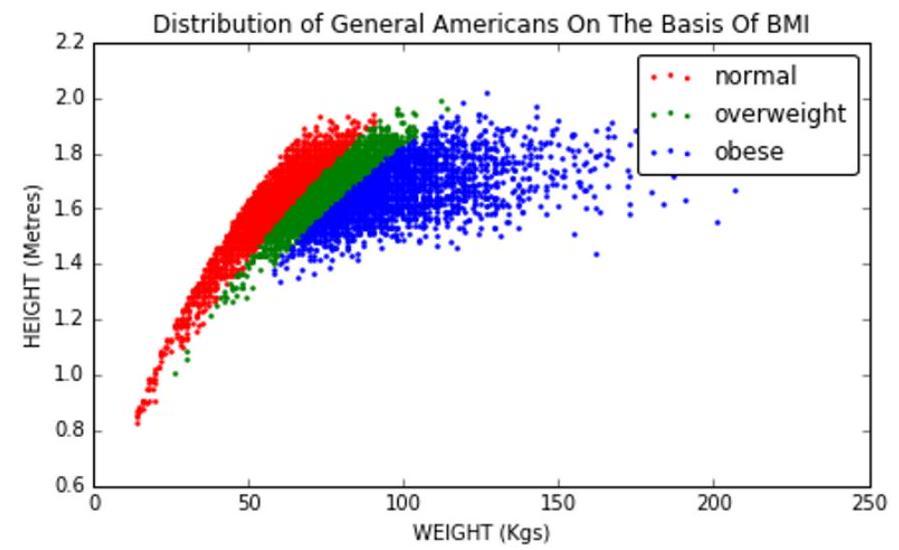
\includegraphics[width=\textwidth]{2025_03_17_ca60ec0bfd96dcf8e028g-113}
\caption{Height-weight scatter plot, for 1000 representative Americans. Colors illustrate class labels in the BMI distribution.}
\end{figure}

\begin{itemize}
  \item \textit{Obese}: over 30.
\end{itemize}

Thus I am considered to be in normal range, with another dozen pounds to gain before I officially become overweight. Figure 4.1 plots where a representative group of Americans sit in height-weight space according to this scale. Each point in this scatter plot is a person, colored according to their weight classification by BMI. Regions of seemingly solid color are so dense with people that the dots overlap. Outlier points to the right correspond to the heaviest individuals.

The BMI is an example of a very successful statistic/scoring function. It is widely used and generally accepted, although some in the public health field quibble that better statistics are available.

The logic for the BMI is almost sound. The square of height should be proportional to area. But mass should grow proportional to the \textit{volume}, not area, so why is it not \textit{mass/height}$^3$? Historically, BMI was designed to correlate with the percentage of body fat in an individual, which is a much harder measurement to make than height and weight. Experiments with several simple scoring functions, including \textit{m/l} and \textit{m/l}$^3$ revealed that BMI works best.

It is very interesting to look at BMI distributions for extreme populations. Consider professional athletes in American football (NFL) and basketball (NBA):
\begin{itemize}
  \item Basketball players are notoriously tall individuals. They also have to run up and down the court all day, promoting superior fitness.
  \item American football players are notoriously heavy individuals. In particular, linemen exist only to block or move other linemen, thus placing a premium on bulk.
\end{itemize}

Let's look at some data. Figure 4.2 shows the BMI distributions of basketball and football players, by sport. And indeed, almost all of the basketball players

\begin{figure}[h]
\centering
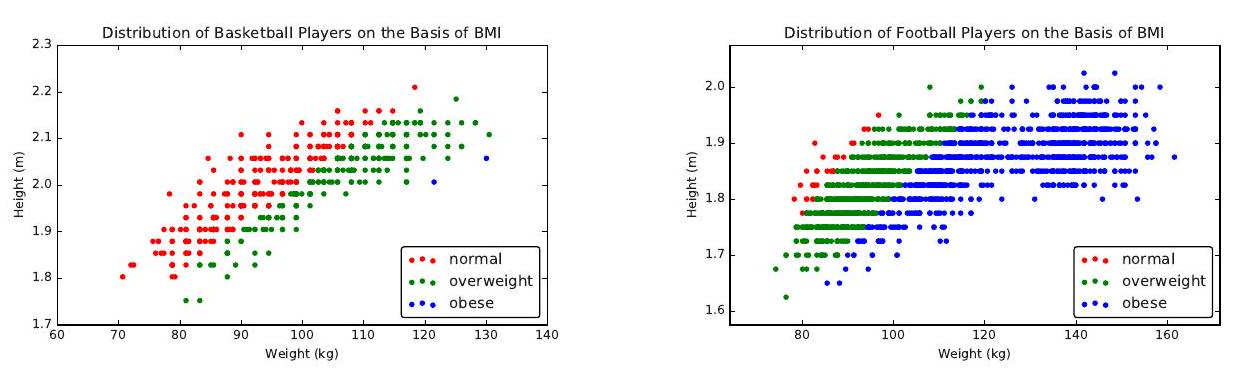
\includegraphics[width=\textwidth]{2025_03_17_ca60ec0bfd96dcf8e028g-114(2)}
\caption{BMI distributions of professional basketball (left) and football (right) players.}
\end{figure}

\begin{figure}[h]
\centering
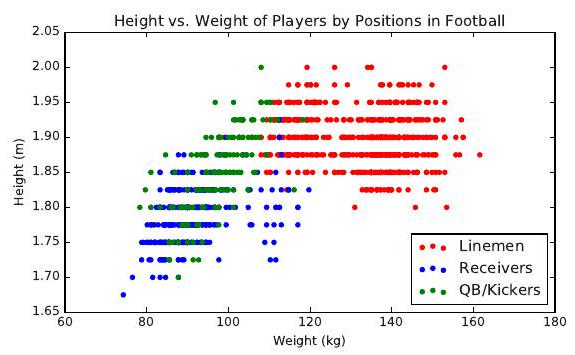
\includegraphics[width=\textwidth]{2025_03_17_ca60ec0bfd96dcf8e028g-114}
\caption{Position in basketball (left) and football (right) is largely determined by size.}
\end{figure}

have normal BMI despite their very abnormal heights. And the football players are almost uniformly animals, with most scored as obese despite the fact that they are also well-conditioned athletes. These football players are generally optimized for strength, instead of cardiovascular fitness.

In Chapter 6, we will discuss visualization techniques to highlight the presentation of data, but let's start to develop our aesthetic here. We use \textit{scatter plots} to show each individual as a point in height-weight space, with labels (weight class or player position) shown as colors.

The breakdown of BMI by position is also revealing, and shown in Figure 4.3. In basketball, the guards are quick and sleek while the centers are tall and intimidating. So all of these positions segregate neatly by size. In football, the skill players (the quarterbacks, kickers, and punters) prove to be considerably smaller than the sides of beef on the line.

\subsection*{4.2 Developing Scoring Systems}
\textit{Scores} are functions that map the features of each entity to a numerical value of merit. This section will look at the basic approaches for building effective scoring systems, and evaluating them.

\subsection*{4.2.1 Gold Standards and Proxies}
Historically, paper currencies were backed with gold, meaning that one paper dollar could always be traded in for \$1 worth of gold. This was why we knew that our money was worth more than the paper it was printed on.

In data science, a \textit{gold standard} is a set of labels or answers that we trust to be correct. In the original formulation of BMI, the gold standard was the body fat percentages carefully measured on a small number of subjects. Of course, such measurements are subject to some error, but by defining these values to be the gold standard for fitness we accept them to be the right measure. In gold we trust.

The presence of a gold standard provides a rigorous way to develop a good scoring system. We can use curve-fitting technique like linear regression (to be discussed in Section 9.1) to weigh the input features so as to best approximate the "right answers" on the gold standard instances.

But it can be hard to find real gold standards. \textit{Proxies} are easier-to-find data that \textit{should} correlate well with the desired but unobtainable ground truth. BMI was designed to be a proxy for body fat percentages. It is easily computable from just height and weight, and does a pretty good job correlating with body fat. This means it is seldom necessary to test buoyancy in water tanks or "pinch an inch" with calipers, more intrusive measures that directly quantify the extent of an individual's flab.

Suppose I wanted to improve the grading system I use for next year's data science course. I have student data from the previous year, meaning their scores on homework and tests, but I don't really have a gold standard on what grades these students \textit{deserved}. I have only the grade I gave them, which is meaningless if I am trying to improve the system.

I need a proxy for their unknown "real" course merit. A good candidate for this might be each student's cumulative GPA in their \textit{other} courses. Generally speaking, student performance should be conserved across courses. If my scoring system hurts the GPA of the best students and helps the lower tier, I am probably doing something wrong.

Proxies are particularly good when evaluating scoring/ranking systems. In our book \textit{Who's Bigger?} \cite{\cite{skiena2013bigger}} we used Wikipedia to rank historical figures by "significance." We did not have any gold standard significance data measuring how important these people \textit{really} were. But we used several proxies to evaluate how we were doing to keep us honest:
\begin{itemize}
  \item The prices that collectors will pay for autographs from celebrities \textit{should} generally correlate with the celebrity's significance. The higher the price people are willing to pay, the bigger the star.
  \item The statistics of how good a baseball player is \textit{should} generally correlate with the player's significance. The better the athlete, the more important they are likely to be.
  \item Published rankings appearing in books and magazines list the top presidents, movie stars, singers, authors, etc. Presidents ranked higher by historians should generally be ranked higher by us. Such opinions, in aggregate, should generally correlate with the significance of these historical figures.
\end{itemize}
We will discuss the workings of our historical significance scores in greater detail in Section 4.7.
```
%---- Page End Break Here ---- Page : 104
```latex
\begin{itemize}
    \item \textit{Sports contest results}: Typical sporting events, be they football games or chess matches, pit teams \textit{A} and \textit{B} against each other. Only one of them will win. Thus each match is essentially a binary comparison of merit.
    \item \textit{Votes and polls}: Knowledgeable individuals are often asked to compare options and decide which choice they think is better. In an election, these comparisons are called votes. A major component of certain university rankings come from asking professors: which school is better, \textit{A} or \textit{B}?
\end{itemize}

In the movie \textit{The Social Network}, Facebook’s Mark Zuckerberg is shown getting his start with FaceMash, a website showing viewers two faces and asking them to pick which one is more attractive. His site then ranked all the faces from most to least attractive, based on these paired comparisons.

\begin{itemize}
    \item \textit{Implicit comparisons}: From the right vantage point, feature data can be meaningfully interpreted as pairwise comparisons. Suppose a student has been accepted by both universities \textit{A} and \textit{B}, but opts for \textit{A}. This can be taken as an implicit vote that \textit{A} is better than \textit{B}.
\end{itemize}

What is the right way to interpret collections of such votes, especially where there are many candidates, and not all pairs of players face off against each other? It isn’t reasonable to say the one with the most wins wins, because (a) they might have competed in more comparisons than other players, and (b) they might have avoided strong opponents and beaten up only inferior competition.

The \textit{Elo system} starts by rating all players, presumably equally, and then incrementally adjusts each player’s score in response to the result of each match, according to the formula:

$$
r^{\prime}(A) = r(A) + k(S_A - \mu_A)
$$

where

\begin{itemize}
    \item \(r(A)\) and \(r^{\prime}(A)\) represent the previous and updated scores for player \textit{A}.
    \item \(k\) is a fixed parameter reflecting the maximum possible score adjustment in response to a single match. A small value of \(k\) results in fairly static rankings, while using too large a \(k\) will cause wild swings in ranking based on the latest match.
    \item \(S_A\) is the scoring result achieved by player \textit{A} in the match under consideration. Typically, \(S_A = 1\) if \textit{A} won, and \(S_A = -1\) if \textit{A} lost.
    \item \(\mu_A\) was the expected result for \textit{A} when competing against \textit{B}. If \textit{A} has exactly the same skill level as \textit{B}, then presumably \(\mu_A = 0\). But suppose that \textit{A} is a champion and \textit{B} is a beginner or chump. Our expectation is that \textit{A} should almost certainly win in a head-to-head matchup, so \(\mu_A > 0\) and is likely to be quite close to 1.
\end{itemize}

\begin{figure}[h]
    \centering
    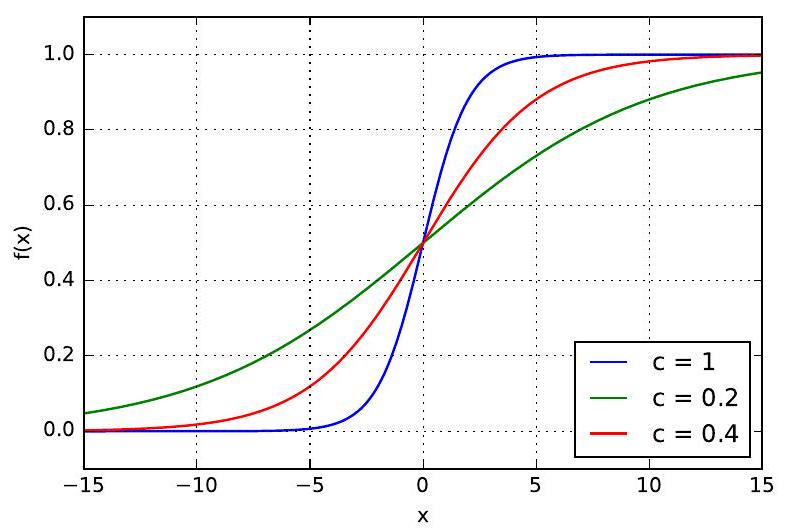
\includegraphics[max width=\textwidth]{2025_03_17_ca60ec0bfd96dcf8e028g-122}
    \caption{The shape of the logit function, for three different values for \(c\).}
\end{figure}

All is clear here except how to determine \(\mu_A\). Given an estimate of the probability that \textit{A} beats \textit{B} \((P_{A>B})\), then

$$
\mu_A = 1 \cdot P_{A>B} + (-1) \cdot (1 - P_{A>B}).
$$

This win probability clearly depends on the magnitude of the skill difference between players \textit{A} and \textit{B}, which is exactly what is supposed to be measured by the ranking system. Thus \(x = r(A) - r(B)\) represents this skill difference.

To complete the Elo ranking system, we need a way to take this real variable \(x\) and convert it to a meaningful probability. This is an important problem we will repeatedly encounter in this book, solved by a bit of mathematics called the \textit{logit function}.

\section*{The Logit Function}
Suppose we want to take a real variable \(-\infty < x < \infty\) and convert it to a probability \(0 \leq p \leq 1\). There are many ways one might imagine doing this, but a particularly simple transformation is \(p = f(x)\), where

$$
f(x) = \frac{1}{1 + e^{-cx}}
$$

The shape of the logit function \(f(x)\) is shown in Figure 4.5. Particularly note the special cases at the mid and endpoints:

\begin{itemize}
    \item When two players are of equal ability, \(x = 0\), and \(f(0) = \frac{1}{2}\), reflects that both players have an equal probability of winning.
    \item When player \textit{A} has a vast advantage, \(x \rightarrow \infty\), and \(f(\infty) = 1\), defining that \textit{A} is a lock to win the match.
\end{itemize}

\begin{figure}[h]
    \centering
    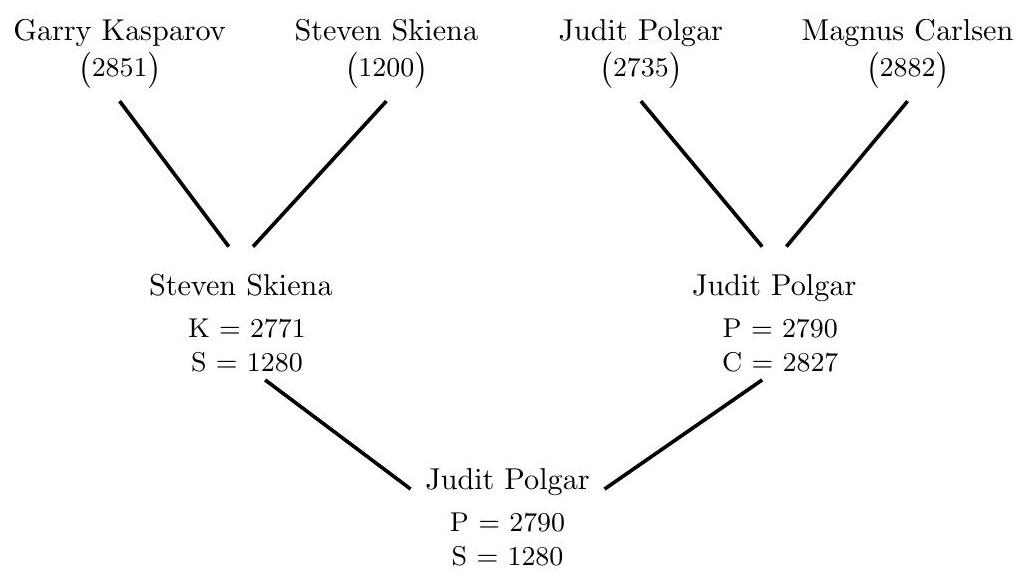
\includegraphics[max width=\textwidth]{2025_03_17_ca60ec0bfd96dcf8e028g-123}
    \caption{Changes in ELO scores as a consequence of an unlikely chess tournament.}
\end{figure}

\begin{itemize}
    \item When player \textit{B} has a vast advantage, \(x \rightarrow -\infty\), and \(f(-\infty) = 0\), denoting that \textit{B} is a lock to win the match.
\end{itemize}

These are exactly the values we want if \(x\) measures the skill difference between the players.

The logit function smoothly and symmetrically interpolates between these poles. The parameter \(c\) in the logit function governs how steep the transition is. Do small differences in skill translate into large differences in the probability of winning? For \(c = 0\), the landscape is as flat as a pancake: \(f(x) = \frac{1}{2}\) for all \(x\). The larger \(c\) is, the sharper the transition, as shown in Figure 4.5. Indeed, \(c = \infty\) yields a step function from 0 to 1.

Setting \(c = 1\) is a reasonable start, but the right choice is domain specific. Observing how often a given skill-difference magnitude results in an upset (the weaker party winning) helps specify the parameter. The Elo Chess ranking system was designed so that \(r(A) - r(B) = 400\) means that \textit{A} has ten times the probability of winning than \textit{B}.

Figure 4.6 illustrates Elo computations, in the context of a highly unlikely tournament featuring three of the greatest chess players in history, and one low-ranked patzer. Here \(k = 40\), implying a maximum possible scoring swing of 80 points as a consequence of any single match. The standard logit function gave Kasparov a probability of 0.999886 of beating Skiena in the first round, but through a miracle akin to raising Lazarus the match went the other way. As a consequence, 80 points went from Kasparov’s ranking to mine.

On the other side of the bracket two real chess champions did battle, with the more imaginable upset by Polgar moving only 55 points. She wiped the floor with me the final round, an achievement so clearly expected that she gained essentially zero rating points. The Elo method is very effective at updating ratings in response to surprise, not just victory.

\begin{center}
    \begin{tabular}{l|ccccll}
        1 & A & B & A & A & \text{A: 5} \\
        2 & C & A & B & B & \text{B: 8} \\
        3 & B & C & C & D & \text{C: 12} \\
        4 & D & D & E & C & \text{D: 16} \\
        5 & E & E & D & E & \text{E: 19} \\
    \end{tabular}
\end{center}

\begin{figure}
    \centering
    \caption{Borda’s method for constructing the consensus ranking of \{A, B, C, D, E\} from a set of four input rankings, using linear weights.}
\end{figure}

\subsection*{4.4.2 Merging Rankings}
Any single numeric feature \(f\), like height, can seed \(\binom{n}{2}\) pairwise comparisons among \(n\) items, by testing whether \(f(A) > f(B)\) for each pair of items \(A\) and \(B\). We could feed these pairs to the Elo method to obtain a ranking, but this would be a silly way to think about things. After all, the result of any such analysis would simply reflect the sorted order of \(f\).

Integrating a collection of rankings by several different features makes for a more interesting problem, however. Here we interpret the sorted order of the \(i\)th feature as defining a permutation \(P_i\) on the items of interest. We seek the consensus permutation \(P\), which somehow best reflects all of the component permutations \(P_1, \ldots, P_k\).

This requires defining a distance function to measure the similarity between two permutations. A similar issue arose in defining the Spearman rank correlation coefficient (see Section 2.3.1), where we compared two variables by the measure of agreement in the relative order of the elements.\footnote{Observe the difference between a similarity measure and a distance metric. In correlation, the scores get bigger as elements get more similar, while in a distance function the difference goes to zero. Distance metrics will be discussed more thoroughly in Section 10.1.1.}

\textit{Borda’s method} creates a consensus ranking from multiple other rankings by using a simple scoring system. In particular, we assign a cost or weight to each of the \(n\) positions in the permutation. Then, for each of the \(n\) elements, we sum up the weights of its positions over all of the \(k\) input rankings. Sorting these \(n\) scores determines the final consensus ranking.

All is now clear except for the mapping between positions and costs. The simplest cost function assign \(i\) points for appearing in the \(i\)th position in each permutation, i.e. we sum up the ranks of the element over all permutations. This is what we do in the example of Figure 4.7. Item \textit{A} gets \(3 \cdot 1 + 1 \cdot 2 = 5\) points on the strength of appearing first in three rankings and second in one. Item \textit{C} finishes with 12 points by finishing 2, 3, 3, and 4. The final consensus ranking of \{A, B, C, D, E\} integrates all the votes from all input rankings, even though the consensus disagrees at least in part with all four input rankings.

But it is not clear that using linear weights represents the best choice, because it assumes uniform confidence in our accuracy to position elements throughout the permutation. Typically, we will know the most about the merits of our top choices, but will be fairly fuzzy about exactly how those near the middle order among themselves. If this is so, a better approach might be to award more points for the distinction between 1st and 2nd than between 110th and 111th.

This type of weighting is implicitly performed by a bell-shaped curve. Suppose we sample \(n\) items at equal intervals from a normal distribution, as shown in Figure 4.8. Assigning these \(x\) values as the positional weights produces more spread at the highest and lowest ranks than the center. The tail regions really are as wide as they appear for these 50 equally-spaced points: recall that 95\% of the probability mass sits within \(2\sigma\) of the center.

\begin{figure}
    \centering
    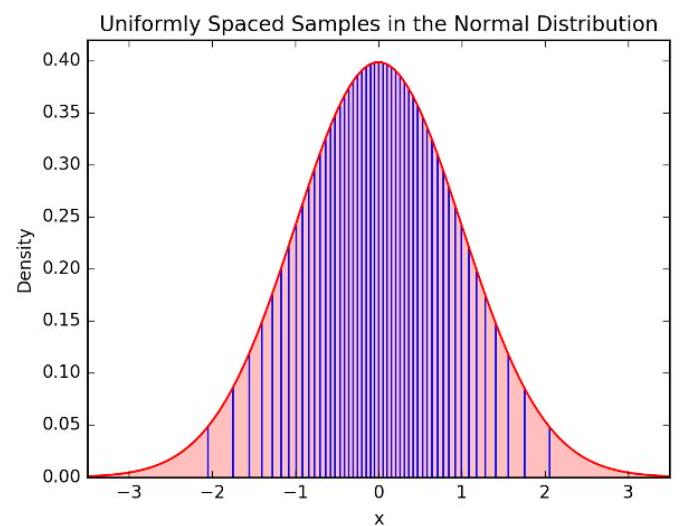
\includegraphics[max width=\textwidth]{2025_03_17_ca60ec0bfd96dcf8e028g-125}
    \caption{Equally-spaced values by the normal distribution are closer in the middle than the ends, making appropriate weights for Borda’s method.}
\end{figure}

Alternately, if our confidence is not symmetric, we could sample from the half-normal distribution, so the tail of our ranks is weighted by the peak of the normal distribution. This way, there is the greatest separation among the highest-ranked elements, but little distinction among the elements of the tail.

Your choice of weighting function here is domain dependent, so pick one that seems to do a good job on your problem. Identifying the very \textit{best} cost function turns out to be an ill-posed problem. And strange things happen when we try to design the perfect election system, as will be shown in Section 4.6.

\subsection*{4.4.3 Digraph-based Rankings}
Networks provide an alternate way to think about a set of votes of the form “\textit{A} ranks ahead of \textit{B}.” We can construct a directed graph/network where there is a vertex corresponding to each entity, and a directed edge \((A, B)\) for each vote that \textit{A} ranks ahead of \textit{B}.

The optimal ranking would then be a permutation \(P\) of the vertices which violates the fewest number of edges, where edge \((A, B)\) is violated if \textit{B} comes before \textit{A} in the final ranking permutation \(P\).

\begin{figure}
    \centering
    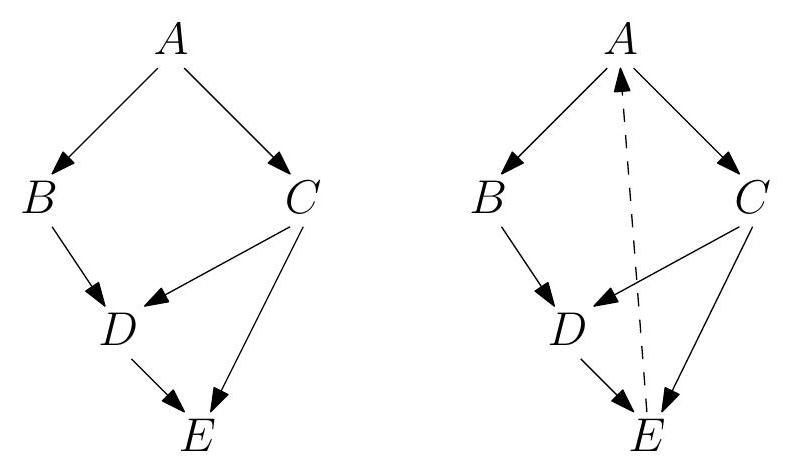
\includegraphics[max width=\textwidth]{2025_03_17_ca60ec0bfd96dcf8e028g-126}
    \caption{Consistently ordered preferences yield an acyclic graph or DAG (left). Inconsistent preferences result in directed cycles, which can be broken by deleting small sets of carefully selected edges, here shown dashed (right).}
\end{figure}

If the votes were totally consistent, then this optimal permutation would violate exactly zero edges. Indeed, this is the case when there are no directed cycles in the graph. A directed cycle like \((A, C)\), \((C, E)\), \((E, A)\) represents an inherent contradiction to any rank order, because there will always be an unhappy edge no matter which order you choose.

A directed graph without cycles is called a \textit{directed acyclic graph} or DAG. An alert reader with a bit of algorithms background will recall that finding this optimal vertex order is called \textit{topologically sorting} the DAG, which can be performed efficiently in linear time. Figure 4.9 (left) is a DAG, and has exactly two distinct orders consistent with the directed edges: \{A, B, C, D, E\} and \{A, C, B, D, E\}.

However, it is exceedingly unlikely that a real set of features or voters will all happen to be mutually consistent. The \textit{maximum acyclic subgraph} problem seeks to find the smallest number of edges to delete to leave a DAG. Removing edge \((E, A)\) suffices in Figure 4.9 (right). Unfortunately, the problem of finding the best ranking here is NP-complete, meaning that no efficient algorithm exists for finding the optimal solution.

But there are natural heuristics. A good clue as to where a vertex \(v\) belongs is the difference \(d_v\) between its in-degree and its out-degree. When \(d_v\) is highly negative, it probably belongs near the front of the permutation, since it dominates many elements but is dominated by only a few. One can build a decent ranking permutation by sorting the vertices according to these differences. Even better is incrementally inserting the most negative (or most positive) vertex \(v\) into its logical position, deleting the edges incident on \(v\), and then adjusting the counts before positioning the next best vertex.

\subsection*{4.4.4 PageRank}
There is a different and more famous method to order the vertices in a network by importance: the PageRank algorithm underpinning Google’s search engine.

The web is constructed of webpages, most of which contain links to other webpages. Your webpage linking to mine is an implicit endorsement that you think my page is pretty good. If it is interpreted as a vote that “you think my page is better than yours,” we can construct the network of links and treat it as a maximum acyclic-subgraph problem, discussed in the previous subsection.

But dominance isn’t really the right interpretation for links on the web. PageRank instead rewards vertices which have the most in-links to it: if all roads lead to Rome, Rome must be a fairly important place. Further, it weighs these in-links by the strength of the source: a link to me from an important page should count for more than one from a spam site.

The details here are interesting, but I will defer a deeper discussion to Section 10.4, when we discuss network analysis. However, I hope this brief introduction to PageRank helps you appreciate the following tale.

\subsection*{4.5 War Story: Clyde’s Revenge}
During my sophomore year of high school, I had the idea of writing a program to predict the outcome of professional football games. I wasn’t all that interested in football as a sport, but I observed several of my classmates betting their lunch money on the outcome of the weekend football games. It seemed clear to me that writing a program which accurately predicted the outcome of football games could have significant value, and be a very cool thing to do besides.

In retrospect, the program I came up with now seems hopelessly crude. My program would average the points scored by team \(x\) and the points allowed by team \(y\) to predict the number of points \(x\) will score against \(y\).

\[ P_x = \frac{((\text{points scored by team } x) + (\text{points allowed by team } y))}{2 \times (\text{games played})} \]

\[ P_y = \frac{((\text{points scored by team } y) + (\text{points allowed by team } x))}{2 \times (\text{games played})} \]

I would then adjust these numbers up or down in response to other factors, particularly home field advantage, round the numbers appropriately, and call what was left my predicted score for the game.

This computer program, \textit{Clyde}, was my first attempt to build a scoring function for some aspect of the real world. It had a certain amount of logic going for it. Good teams score more points than they allow, while bad teams allow more points than they score. If team \(x\) plays a team \(y\) which has given up a lot of points, then \(x\) should score more points against \(y\) than it does against teams with better defenses. Similarly, the more points team \(x\) has scored against the rest of the league, the more points it is likely to score against \(y\).

Of course, this crude model couldn’t capture all aspects of football reality. Suppose team \(x\) has been playing all stiffs thus far in the season, while team \(y\) has been playing the best teams in the league. Team \(y\) might be a much better team than \(x\) even though its record so far is poor. This model also ignores any injuries a team is suffering from, whether the weather is hot or cold, and whether the team is hot or cold. It disregards all the factors that make sports inherently unpredictable.

And yet, even such a simple model can do a reasonable job of predicting the outcome of football games. If you compute the point averages as above, and give the home team an additional three points as a bonus, you will pick the winner in almost two-thirds of all football games. Compare this to the even cruder model of flipping a coin, which predicts only half the games correctly. That was the first major lesson \textit{Clyde} taught me:

\begin{quote}
    \textit{Even crude mathematical models can have real predictive power.}
\end{quote}

As an audacious 16 year-old, I wrote to our local newspaper, \textit{The New Brunswick Home News}, explaining that I had a computer program to predict football game results and was ready to offer them the exclusive opportunity to publish my predictions each week. Remember that this was back in 1977, well before personal computers had registered on the public consciousness. In those days, the idea of a high school kid actually \textit{using} a computer had considerable gee-whiz novelty value. To appreciate how much times have changed, check out the article the paper published about \textit{Clyde} and I in Figure 4.10.

I got the job. \textit{Clyde} predicted the outcome of each game in the 1977 National Football League. As I recall, \textit{Clyde} and I finished the season with the seemingly impressive record of 135–70. Each week, they would compare my predictions against those of the newspaper’s sportswriters. As I recall, we all finished within a few games of each other, although most of the sportswriters finished with better records than the computer.

The \textit{Home News} was so impressed by my work that they didn’t renew me the following season. However, \textit{Clyde}’s picks for the 1978 season were published in the \textit{Philadelphia Inquirer}, a much bigger newspaper. I didn’t have the column to myself, though. Instead, the \textit{Inquirer} included me among ten amateur and professional prognosticators, or touts. Each week we had to predict the outcomes of four games against the point spread.

The point spread in football is a way of handicapping stronger teams for betting purposes. The point spread is designed to make each game a 50/50 proposition, and hence makes predicting the outcome of games much harder.

\textit{Clyde} and I didn’t do very well against the spread during the 1978 National Football League season, and neither did most of the other \textit{Philadelphia Inquirer} touts. We predicted only 46\% of our games correctly against the spread, a performance good (or bad) enough to finish 7th out of the ten published prognosticators. Picking against the spread taught me a second major life lesson:

\begin{quote}
    \textit{Crude mathematical models do not have real predictive power when there is real money on the line.}
\end{quote}

\begin{figure}
    \centering
    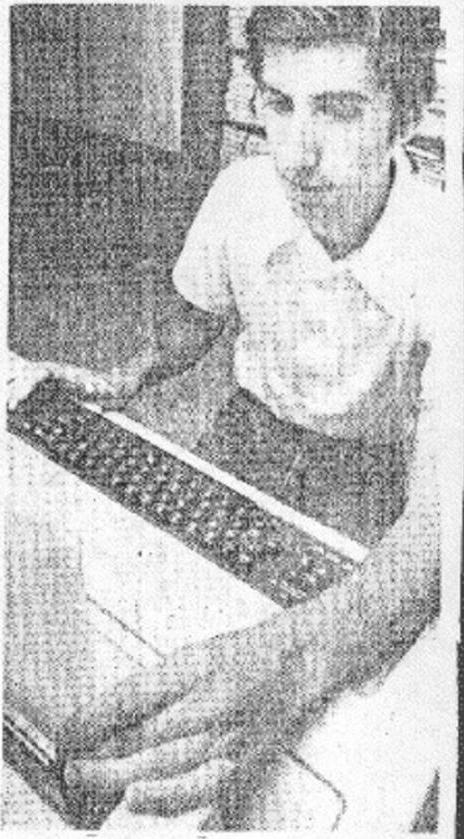
\includegraphics[max width=\textwidth]{2025_03_17_ca60ec0bfd96dcf8e028g-129}
    \caption{My first attempt at mathematical modeling.}
\end{figure}

So Clyde was not destined to revolutionize the world of football prognostication. I pretty much forgot about it until I assigned the challenge of predicting the Super Bowl as a project in my data science class. The team that got the job was made up of students from India, meaning they knew much more about cricket than American football when they started.

Still, they rose to the challenge, becoming fans as they built a large data set on the outcome of every professional and college game played over the past ten years. They did a logistic regression analysis over 142 different features including rushing, passing, and kicking yardage, time of possession, and number of punts. They then proudly reported to me the accuracy of their model: correct predictions on 51.52\% of NFL games.\\ “What!” I screamed, “That’s terrible!” “Fifty percent is what you get by flipping a coin. Try averaging the points scored and yielded by the two teams, and give three points to the home team. How does that simple model do?”

On their data set, this Clyde-light model picked 59.02\% of all games correctly, much much better than their sophisticated-looking machine learning model. They had gotten lost in the mist of too many features, which were not properly normalized, and built using statistics collected over too long a history to be representative of the current team composition. Eventually, the students managed to come up with a PageRank-based model that did a little bit better (60.61\%), but Clyde did almost as well serving as a baseline model.

There are several important lessons here. First, garbage in, garbage out. If you don’t prepare a clean, properly normalized data set, the most advanced machine learning algorithms can’t save you. Second, simple scores based on a modest amount of domain-specific knowledge can do surprisingly well. Further, they help keep you honest. Build and evaluate simple, understandable baselines before you invest in more powerful approaches. Clyde going baseline left their machine learning model defenseless.

\subsection*{4.6 Arrow’s Impossibility Theorem}
We have seen several approaches to construct rankings or scoring functions from data. If we have a gold standard reporting the “right” relative order for at least some of the entities, then this could be used to train or evaluate our scoring function to agree with these rankings to the greatest extent possible.

But without a gold standard, it can be shown that no best ranking system exists. This is a consequence of \textit{Arrow’s impossibility theorem}, which proves that no election system for aggregating permutations of preferences satisfies the following desirable and innocent-looking properties:

\begin{itemize}
    \item The system should be complete, in that when asked to choose between alternatives \textit{A} and \textit{B}, it should say (1) \textit{A} is preferred to \textit{B}, (2) \textit{B} is preferred to \textit{A}, or (3) there is equal preference between them.
\end{itemize}

\begin{center}
    \begin{tabular}{c|ccc}
        Voter & Red & Green & Blue \\
        \hline
        x & 1 & 2 & 3 \\
        y & 2 & 3 & 1 \\
        z & 3 & 1 & 2 \\
        \hline
    \end{tabular}
\end{center}

\begin{figure}
    \centering
    \caption{Preference rankings for colors highlighting the loss of transitivity. Red is preferred to green and green preferred to blue, yet blue is preferred to red.}
\end{figure}

\begin{itemize}
    \item The results should be transitive, meaning if \textit{A} is preferred to \textit{B}, and \textit{B} is preferred to \textit{C}, then \textit{A} must be preferred to \textit{C}.
    \item If every individual prefers \textit{A} to \textit{B}, then the system should prefer \textit{A} to \textit{B}.
    \item The system should not depend only upon the preferences of one individual, a dictator.
    \item The preference of \textit{A} compared to \textit{B} should be independent of preferences for any other alternatives, like \textit{C}.
\end{itemize}

Figure 4.11 captures some of the flavor of Arrow’s theorem, and the non-transitive nature of “rock-paper-scissors” type ordering. It shows three voters (\textit{x}, \textit{y}, and \textit{z}) ranking their preferences among colors. To establish the preference among two colors \textit{a} and \textit{b}, a logical system might compare how many permutations rank \textit{a} before \textit{b} as opposed to \textit{b} before \textit{a}. By this system, red is preferred to green by \textit{x} and \textit{y}, so red wins. Similarly, green is preferred to blue by \textit{x} and \textit{z}, so green wins. By transitivity, red should be preferred to blue by implication on these results. Yet \textit{y} and \textit{z}, prefer blue to red, violating an inherent property we want our election system to preserve.

Arrow’s theorem is very surprising, but does it mean that we should give up on rankings as a tool for analyzing data? Of course not, no more than Arrow’s theorem means that we should give up on democracy. Traditional voting systems based on the idea that the \textit{majority rules} generally do a good job of reflecting popular preferences, once appropriately generalized to deal with large numbers of candidates. And the techniques in this chapter generally do a good job of ranking items in interesting and meaningful ways.

\textit{Take-Home Lesson}: We do not seek correct rankings, because this is an ill-defined objective. Instead, we seek rankings that are useful and interesting.

\subsection*{4.7 War Story: Who’s Bigger?}
My students sometimes tell me that I am history. I hope this isn’t true quite yet, but I am very interested in history, as is my former postdoc Charles Ward. Charles and I got to chatting about who the most significant figures in history were, and how you might measure this. Like most people, we found our answers in Wikipedia.

Wikipedia is an amazing thing, a distributed work product built by over 100,000 authors which somehow maintains a generally sound standard of accuracy and depth. Wikipedia captures an astonishing amount of human knowledge in an open and machine-readable form.

We set about using the English Wikipedia as a data source to base historical rankings on. Our first step was to extract feature variables from each person’s Wikipedia page that should clearly correlate with historical significance. This included features like:

\begin{itemize}
    \item \textit{Length}: Most significant historical figures should have longer Wikipedia pages than lesser mortals. Thus article length in words provides a natural feature reflecting historical wattage, to at least some degree.
    \item \textit{Hits}: The most significant figures have their Wikipedia pages read more often than others, because they are of greater interest to a larger number of people. My Wikipedia page gets hit an average of twenty times per day, which is pretty cool. But Issac Newton’s page gets hit an average of 7700 times per day, which is a hell of a lot better.
    \item \textit{PageRank}: Significant historical figures interact with other significant historical figures, which get reflected as hyperlink references in Wikipedia articles. This defines a directed graph where the vertices are articles, and the directed edges hyperlinks. Computing the PageRank of this graph will measure the centrality of each historical figure, which correlates well with significance.
\end{itemize}

All told, we extracted six features for each historical figure. Next, we normalized these variables before aggregating, essentially by combining the underlying rankings with normally-distributed weights, as suggested in Section 4.4.2. We used a technique called \textit{statistical factor analysis} related to principal component analysis (discussed in Section 8.5.2), to isolate two factors that explained most of the variance in our data. A simple linear combination of these variables gave us a scoring function, and we sorted the scores to determine our initial ranking, something we called \textit{fame}.

The top twenty figures by our fame score are shown in Figure 4.12 (right). We studied these rankings and decided that it didn’t really capture what we wanted it to. The top twenty by fame included pop musicians like Madonna and Michael Jackson, and three contemporary U.S. presidents. It was clear that contemporary figures ranked far higher than we thought they should: our scoring function was capturing current fame much more than historical significance.

Our solution was to decay the scores of contemporary figures to account for the passage of time. That a current celebrity gets a lot of Wikipedia hits is impressive, but that we still care about someone who died 300 years ago is much more impressive. The top twenty figures after age correction are shown in Figure 4.12 (left).
```
%---- Page End Break Here ---- Page : 116
%---- Page End Break Here ---- Page : 116

\begin{center}
\begin{tabular}{|r|l|c|l|}
\hline
Signif & \multicolumn{1}{|c|}{Name} & \multicolumn{1}{|c|}{Fame} & \multicolumn{1}{|c|}{Person} \\
\hline
1 & Jesus & 1 & George W. Bush \\
2 & Napoleon &  &  \\
3 & William Shakespeare & 2 & Barack Obama \\
4 & Muhammad & 3 & Jesus \\
5 & Abraham Lincoln & 4 & Adolf Hitler \\
6 & George Washington & 5 & Ronald Reagan \\
7 & Adolf Hitler & 6 & Bill Clinton \\
8 & Aristotle & 7 & Napoleon \\
9 & Alexander the Great &  &  \\
10 & Thomas Jefferson & 8 & Michael Jackson \\
11 & Henry VIII & 9 & W. Shakespeare \\
12 & Elizabeth I & 10 & Elvis Presley \\
13 & Julius Caesar & 11 & Muhammad \\
14 & Charles Darwin & 12 & Joseph Stalin \\
15 & Karl Marx & 13 & Abraham Lincoln \\
16 & Martin Luther & 14 & G. Washington \\
17 & Queen Victoria & 15 & Albert Einstein \\
18 & Joseph Stalin & 16 & John F. Kennedy \\
19 & Theodore Roosevelt &  &  \\
20 & Albert Einstein & 17 & Elizabeth II \\
 & 18 & John Paul II &  \\
 & 19 & Madonna &  \\
20 & Britney Spears &  &  \\
\hline
\end{tabular}
\end{center}

\begin{figure}[h]
\centering
\caption{The top 20 historical figures, ranked by significance (left) and contemporary fame (right).}
\end{figure}

Now \emph{this} was what we were looking for! We validated the rankings using whatever proxies for historical significance we could find: other published rankings, autograph prices, sports statistics, history textbooks, and Hall of Fame election results. Our rankings showed a strong correlation against all of these proxies.

Indeed, I think these rankings are wonderfully revealing. We wrote a book describing all kinds of things that could be learned from them \cite{SW13}. I proudly encourage you to read it if you are interested in history and culture. The more we studied these rankings, the more I was impressed in their general soundness.

That said, our published rankings did not meet with universal agreement. Far from it. Dozens of newspaper and magazine articles were published about our rankings, many quite hostile. Why didn't people respect them, despite our extensive validation? In retrospect, most of the flack we fielded came for three different reasons:

\begin{itemize}
  \item \emph{Differing implicit notions of significance}: Our methods were designed to measure \emph{meme-strength}, how successfully these historical figures were propagating their names through history. But many readers thought our methods should capture notions of historical \emph{greatness}. Who was most important, in terms of changing the world? And do we mean world or just the English-speaking world? How can there be no Chinese or Indian figures on the list when they represent over $30\%$ of the world's population?\\
We must agree on what we are trying to measure before measuring it. Height is an excellent measure of size, but it does not do a good job of capturing obesity. However, height is very useful to select players for a basketball team.
  \item \emph{Outliers}: Sniff tests are important to evaluating the results of an analysis. With respect to our rankings, this meant checking the placement of people we knew, to confirm that they fell in reasonable places.\\
I felt great about our method's ranking of the vast majority of historical figures. But there were a few people who our method ranked higher than any reasonable person would, specifically President George W. Bush (36) and teenage TV star Hilary Duff (1626). One could look at these outliers and dismiss the entire thing. But understand that we ranked almost 850,000 historical figures, roughly the population of San Francisco. A few cherry-picked bad examples must be put in the proper context.
  \item \emph{Pigeonhole constraints}: Most reviewers saw only the rankings of our top 100 figures, and they complained about exactly where we placed people and who didn't make the cut. The women's TV show \emph{The View} complained we didn't have enough women. I recall British articles complaining we had Winston Churchill (37) ranked too low, South African articles that thought we dissed Nelson Mandela (356), Chinese articles saying we didn't have enough Chinese, and even a Chilean magazine whining about the absence of Chileans.\\
Some of this reflects cultural differences. These critics had a different implicit notion of significance than reflected by English Wikipedia. But much of it reflects the fact that there are exactly one hundred places in the top 100. Many of the figures they saw as missing were just slightly outside the visible horizon. For every new person we moved into the top hundred, we had to drop somebody else out. But readers almost never suggested names that should be omitted, only those who had to be added.
\end{itemize}

What is the moral here? Try to anticipate the concerns of the audience for your rankings. We were encouraged to explicitly call our measure \emph{meme-strength} instead of \emph{significance}. In retrospect, using this less-loaded name would have permitted our readers to better appreciate what we were doing. We probably also should have discouraged readers from latching on to our top 100 rankings, and instead concentrate on relative orderings within groups of interest: who were the top musicians, scientists, and artists? This might have proved less controversial, better helping people build trust in what we were doing.

\subsection*{4.8 Chapter Notes}
Langville and Meyer \cite{\cite{langville2012who}} provide a thorough introduction to most of the ranking methods discussed here, including Elo and PageRank.

%---- Page End Break Here ---- Page : 118

One important topic not covered in this chapter is \emph{learning to rank} methods, which exploit gold standard ranking data to train appropriate scoring functions. Such ground truth data is generally not available, but proxies can sometimes be found. When evaluating search engines, the observation that a user clicked the (say) fourth item presented to them can be interpreted as a vote that it should have been higher ranked than the three placed above it. SVMrank \cite{\cite{joachims2002optimizing}} presents a method for learning ranking functions from such data.

The heuristic proposed minimizing edge conflicts in a vertex order is due to Eades et. al. \cite{\cite{eades1993fast}}. My presentation of Arrow's impossibility theorem is based on notes from Watkins \cite{\cite{watkins2016arrow}}.

The war stories of this chapter were drawn very closely from my books \emph{Calculated Bets} and \emph{Who's Bigger?} Don't sue me for self-plagiarism.

\subsection*{4.9 Exercises}
\section*{Scores and Rankings}
\begin{enumerate}
    \item Let $X$ represent a random variable drawn from the normal distribution defined by $\mu=2$ and $\sigma=3$. Suppose we observe $X=5.08$. Find the Z-score of $x$, and determine how many standard deviations away from the mean that $x$ is.
    
    \item What percentage of the standard normal distribution $(\mu=0, \sigma=1)$ is found in each region?
    \begin{enumerate}
        \item $Z > 1.13$.
        \item $Z < 0.18$.
        \item $Z > 8$.
        \item $|Z| < 0.5$.
    \end{enumerate}
    
    \item Amanda took the Graduate Record Examination (GRE), and scored 160 in verbal reasoning and 157 in quantitative reasoning. The mean score for verbal reasoning was 151 with a standard deviation of 7, compared with mean $\mu=153$ and $\sigma=7.67$ for quantitative reasoning. Assume that both distributions are normal.
    \begin{enumerate}
        \item What were Amanda's Z-scores on these exam sections? Mark these scores on a standard normal distribution curve.
        \item Which section did she do better on, relative to other students?
        \item Find her percentile scores for the two exams.
    \end{enumerate}
    
    \item Identify three successful and well-used scoring functions in areas of personal interest to you. For each, explain what makes it a good scoring function and how it is used by others.
    
    \item Find a data set on properties of one of the following classes of things:
    \begin{enumerate}
        \item The countries of the world.
        \item Movies and movie stars.
        \item Sports stars.
        \item Universities.
    \end{enumerate}
    Construct a sensible ranking function reflecting quality or popularity. How well is this correlated with some external measure aiming at a similar result?
    
    \item Produce two substantially different but sensible scoring functions on the same set of items. How different are the resulting rankings? Does the fact that both have to be sensible constrain rankings to be grossly similar?
    
    \item The scoring systems used by professional sports leagues to select the most valuable player award winner typically involves assigning positional weights to permutations specified by voters. What systems do they use in professional baseball, basketball, and football? Are they similar? Do you think they are sensible?
\end{enumerate}

\section*{Implementation Projects}
\begin{enumerate}
    \item Use Elo ratings to rank all the teams in a sport such as baseball, football, or basketball, which adjusts the rating in response to each new game outcome. How accurately do these Elo ratings predict the results of future contests?
    
    \item Evaluate the robustness of Borda's method by applying $k$ random swaps to each of $m$ distinct copies of the permutation $p=\{1,2, \ldots, n\}$. What is the threshold where Borda's method fails to reconstruct $p$, as a function of $n, k$, and $m$?
\end{enumerate}

\section*{Interview Questions}
\begin{enumerate}
    \item What makes a data set a gold standard?
    \item How can you test whether a new credit risk scoring model works?
    \item How would you forecast sales for a particular book, based on Amazon public data?
\end{enumerate}

\section*{Kaggle Challenges}
\begin{enumerate}
    \item Rating chess players from game positions.\\ \url{https://www.kaggle.com/c/chess}
    \item Develop a financial credit scoring system.\\ \url{https://www.kaggle.com/c/GiveMeSomeCredit}
    \item Predict the salary of a job from its ad.\\ \url{https://www.kaggle.com/c/job-salary-prediction}
\end{enumerate}

\section*{Chapter 5}
\section*{Statistical Analysis}
\begin{quote}
It is easy to lie with statistics, but easier to lie without them.
\end{quote}

\begin{flushright}
— Frederick Mosteller
\end{flushright}

I will confess that I have never had a truly satisfying conversation with a statistician. This is not completely for want of trying. Several times over the years I have taken problems of interest to statisticians, but always came back with answers like "You can't do it that way" or "But it's not independent," instead of hearing "Here is the way you can handle it."

To be fair, these statisticians generally did not appreciate talking with me, either. Statisticians have been thinking seriously about data for far longer than computer scientists, and have many powerful methods and ideas to show for it. In this chapter, I will introduce some of these important tools, like the definitions of certain fundamental distributions and tests for statistical significance. This chapter will also introduce Bayesian analysis, a way to rigorously assess how new data should affect our previous estimates of future events.\\

\begin{figure}[h]
\centering
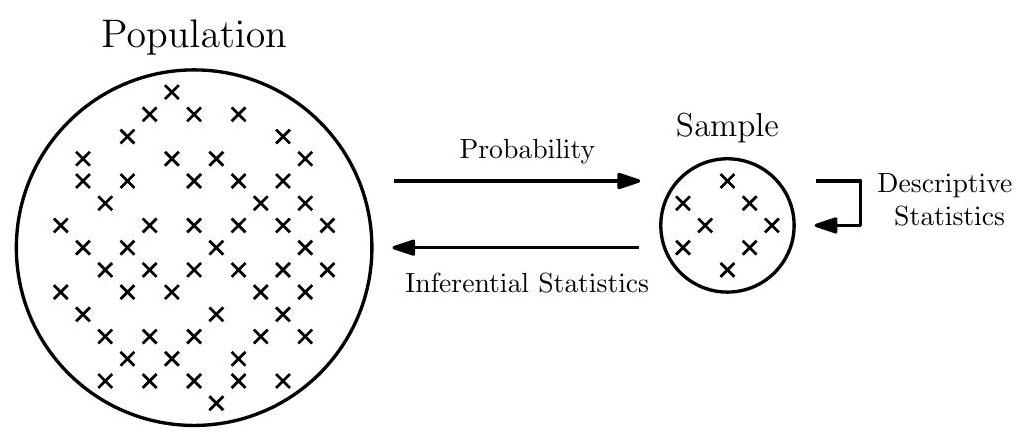
\includegraphics[max width=\textwidth]{2025_03_17_ca60ec0bfd96dcf8e028g-137}
\caption{The central dogma of statistics: analysis of a small random sample enables drawing rigorous inferences about the entire population.}
\end{figure} 

Figure 5.1 illustrates the process of statistical reasoning. There is an underlying population of possible things that we can potentially observe. Only a relatively small subset of them are actually sampled, ideally at random, meaning that we can observe properties of the sampled items. Probability theory describes what properties our sample should have, given the properties of the underlying population. But statistical inference works the other way, where we try to deduce what the full population is like given analysis of the sample.

Ideally, we will learn to think like a statistician: enough so as to remain vigilant and guard against overinterpretation and error, while retaining our confidence to play with data and take it where it leads us.

\subsection*{5.1 Statistical Distributions}
Every variable that we observe defines a particular frequency distribution, which reflects how often each particular value arises. The unique properties of variables like height, weight, and IQ are captured by their distributions. But the shapes of these distributions are themselves not unique: to a great extent, the world's rich variety of data appear only in a small number of classical forms.

These classical distributions have two nice properties: (1) they describe \emph{shapes of frequency distributions that arise often in practice}, and (2) they can often be described mathematically using closed-form expressions with very few parameters. Once abstracted from specific data observations, they become \emph{probability distributions}, worthy of independent study.

Familiarity with the classical probability distributions is important. They arise often in practice, so you should be on the look out for them. They give us a vocabulary to talk about what our data looks like. We will review the most important statistical distributions (binomial, normal, Poisson, and power law) in the sections to follow, emphasizing the properties that define their essential character.

Note that your observed data does not necessarily arise from a particular theoretical distribution just because its shape is similar. Statistical tests can be used to rigorously prove whether your experimentally-observed data reflects samples drawn from a particular distribution.

But I am going to save you the trouble of actually running any of these tests. I will state with high confidence that your real-world data \emph{does not} precisely fit any of the famous theoretical distributions.

Why is that? Understand that the world is a complicated place, which makes measuring it a messy process. Your observations will probably be drawn from multiple sample populations, each of which has a somewhat different underlying distribution. Something funny generally happens at the tails of any observed distribution: a sudden burst of unusually high or low values. Measurements will have errors associated with them, sometimes in weird systematic ways.

But that said, understanding the basic distributions is indeed very important. Each classical distribution is classical for a reason. Understanding these reasons tells you a lot about observed data, so they will be reviewed here.

\begin{figure}[h]
\centering
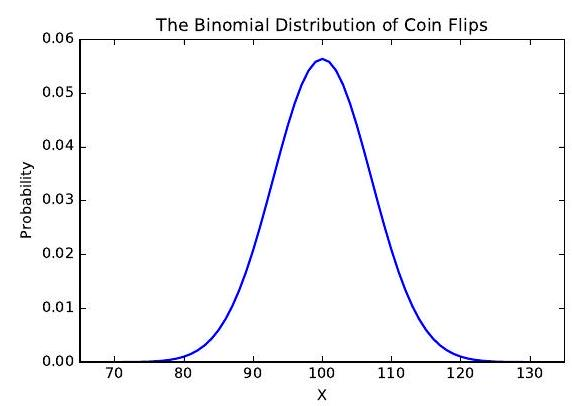
\includegraphics[max width=\textwidth]{2025_03_17_ca60ec0bfd96dcf8e028g-139(1)}
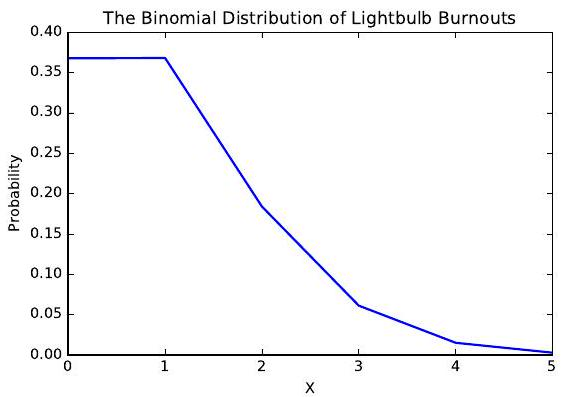
\includegraphics[max width=\textwidth]{2025_03_17_ca60ec0bfd96dcf8e028g-139}
\caption{The binomial distribution can be used to model the distribution of heads in 200 coin tosses with $p=0.5$ (left), and the number of blown lightbulbs in 1000 events with failure probability $p=0.001$ (right).}
\end{figure}

\subsection*{5.1.1 The Binomial Distribution}
Consider an experiment consisting of identical, independent trials which have two possible outcomes $P_{1}$ and $P_{2}$, with the respective probabilities of $p$ and $q=(1-p)$. Perhaps your experiment is flipping fair coins, where the probability of heads $(p=0.5)$ is the same as getting tails $(q=0.5)$. Perhaps it is repeatedly turning on a light switch, where the probability of suddenly discovering that you must change the bulb ($p=0.001$) is much less than that of seeing the light ($q=0.999$).

The \emph{binomial distribution} reports the probability of getting exactly $x P_{1}$ events in the course of $n$ independent trials, in no particular order. Independence is important here: we are assuming the probability of failure of a bulb has no relation to how many times it has previously been used. The pdf for the binomial distribution is defined by:

\[
P(X=x)=\binom{n}{x} p^{x}(1-p)^{(n-x)}
\]

There are several things to observe about the binomial distribution:
\begin{itemize}
  \item \emph{It is discrete}: Both arguments to the binomial distribution ($n$ and $x$) must be integers. The smoothness of Figure 5.2 (left) is an illusion, because $n=200$ is fairly large. There is no way of getting 101.25 heads in 200 coin tosses.
  \item \emph{You probably can explain the theory behind it}: You first encountered the binomial distribution in high school. Remember Pascal's triangle? To end up with exactly $x$ heads in $n$ flips in a particular sequence occurs with probability $p^{x}(1-p)^{(n-x)}$, for each of the $\binom{n}{x}$ distinct flip sequences.
  \item \emph{It is sort of bell-shaped}: For a fair coin $(p=0.5)$, the binomial distribution is perfectly symmetrical, with the mean in the middle. This is not true\\
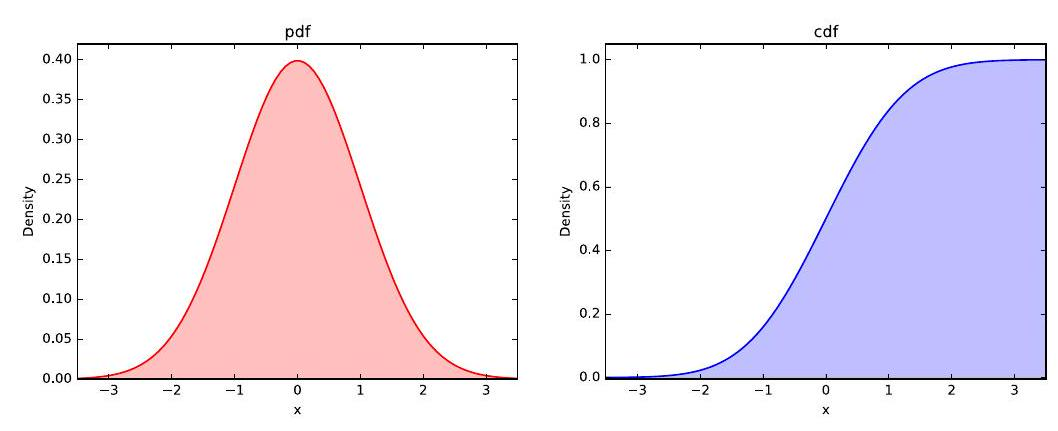
\includegraphics[max width=\textwidth]{2025_03_17_ca60ec0bfd96dcf8e028g-140}
\end{itemize}

Figure 5.3: The probability density function (pdf) of the normal distribution (left) with its corresponding cumulative density function (cdf) on right.\\
in the lightbulb case: if we only turn on the bulb $n=1000$ times, the most likely number of failures will be zero. This rings just half the bell in Figure 5.2. That said, as $n \rightarrow \infty$ we will get a symmetric distribution peaking at the mean.

\begin{itemize}
  \item \emph{It is defined using only two parameters}: All we need are values of $p$ and $n$ to completely define a given binomial distribution.
\end{itemize}

Many things can be reasonably modeled by the binomial distribution. Recall the variance in the performance of a $p=0.300$ hitter discussed in Section 2.2.3. There the probability of getting a hit with each trial was $p=0.3$, with $n=500$ trials per season. Thus the number of hits per season are drawn from a binomial distribution.

Realizing that it was a binomial distribution meant that we really didn't have to use simulation to construct the distribution. Properties like the expected number of hits $\mu=n p=500 \times 0.3=150$ and its standard deviation $\sigma=$ $\sqrt{n p q}=\sqrt{500 \times 0.3 \times 0.7}=10.25$ simply fall out of closed-form formulas that you can look up when needed.

\subsection*{5.1.2 The Normal Distribution}
A great many natural phenomenon are modeled by bell-shaped curves. Measured characteristics like height, weight, lifespan, and IQ all fit the same basic scheme: the bulk of the values lie pretty close to the mean, the distribution is symmetric, and no value is too extreme. In the entire history of the world, there has never been either a 12-foot-tall man or a 140-year-old woman.

The mother of all bell-shaped curves is the \emph{Gaussian} or \emph{normal distribution}, which is completely parameterized by its mean and standard deviation:

\[
P(x)=\frac{1}{\sigma \sqrt{2 \pi}} e^{-(x-\mu)^{2} / 2 \sigma^{2}}
\]

Figure 5.3 shows the pdf and cdf of the normal distribution. There are several things to note:
\begin{itemize}
  \item \emph{It is continuous}: The arguments to the normal distribution (mean $\mu$ and standard deviation $\sigma$ ) are free to arbitrary real numbers, with the lone constraint that $\sigma>0$.
  \item \emph{You probably can't explain where it comes from}: The normal distribution is a generalization of the binomial distribution, where $n \rightarrow \infty$ and the degree of concentration around the mean is specified by the parameter $\sigma$. Take your intuition here from the binomial distribution, and trust that Gauss got his calculations right: the great mathematician worked out the normal distribution for his Ph.D. dissertation. Or consult any decent statistics book if you are really curious to see where it comes from.
  \item \emph{It truly is bell-shaped}: The Gaussian distribution is the platonic example of a bell-shaped curve. Because it operates on a continuous variable (like height) instead of a discrete count (say, the number of events) it is perfectly smooth. Because it goes infinitely in both directions, there is no truncation of the tails at either end. The normal distribution is a theoretical construct, which helps explain this perfection.
  \item \emph{It is also defined using only two parameters}: However, these are different parameters than the binomial distribution! The normal distribution is completely defined by its central point (given by the mean $\mu$ ) and its spread (given by the standard deviation $\sigma$ ). They are the only knobs we can use to tweak the distribution.
\end{itemize}

\section*{What's Normal?}
An amazing number of naturally-occurring phenomenon are modeled by the normal distribution. Perhaps the most important one is measurement error. Every time you measure your weight on a bathroom scale, you will get a somewhat different answer, even if your weight has not changed. Sometimes the scale will read high and other times low, depending upon room temperature and the warping of the floor. Small errors are more likely than big ones, and slightly high is just \index{duality}as likely as slightly low. Experimental error is generally normally distributed as Gaussian noise.

Physical phenomenon like height, weight, and lifespan all have bell-shaped distributions, by similar arguments. Yet the claim that such distributions are normal is usually made too casually, without precisely specifying the underlying population. Is human height normally distributed? Certainly not: men and women have different mean heights and associated distributions. Is male height normally distributed? Certainly not: by including children in the mix and shrinking senior citizens you again have the sum of several different underlying distributions. Is the height of adult males in the United States normal? No, probably not even then. There are non-trivial populations with growth disorders\
%---- Page End Break Here ---- Page : 125
\
\begin{figure}[h]
\centering
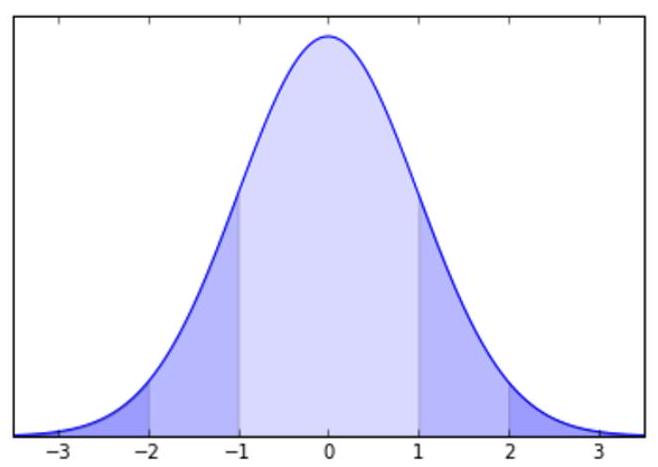
\includegraphics[max width=\textwidth]{2025_03_17_ca60ec0bfd96dcf8e028g-142}
\caption{The normal distribution implies tight bounds on the probability of lying far from the mean. $68 \%$ of the values must lie within one sigma of the mean, and $95 \%$ within $2 \sigma$, and $99.7 \%$ within $3 \sigma$.} 
\end{figure}

like dwarfism and acromegaly, that leave bunches of people substantially shorter and taller than could be explained by the normal distribution.

Perhaps the most famous bell-shaped but non-normal distribution is that of daily returns (percentage price movements) in the financial markets. A big market crash is defined by a large percentage price drop: on October 10, 1987, the Dow Jones average lost $22.61 \%$ of its value. Big stock market crashes occur with much greater frequency than can be accurately modeled by the normal distribution. Indeed, every substantial market crash wipes out a certain number of quants who assumed normality, and inadequately insured against such extreme events. It turns out that the logarithm of stock returns proves to be normally distributed, resulting in a distribution with far fatter tails than normal.

Although we must remember that bell-shaped distributions are not always normal, making such an assumption is a reasonable way to start thinking in the absence of better knowledge.

\subsection*{5.1.3 Implications of the Normal Distribution}
Recall that the mean and standard deviation together always roughly characterize any frequency distribution, as discussed in Section 2.2.4 But they do a spectacularly good job of characterizing the normal distribution, because they define the normal distribution.

Figure 5.4 illustrates the famous $68 \%-95 \%-99.7 \%$ rule of the normal distribution. Sixty-eight percent of the probability mass must lie within the region $\pm 1 \sigma$ of the mean. Further, $95 \%$ of the probability is within $2 \sigma$, and $99.7 \%$ within $3 \sigma$.

This means that values far from the mean (in terms of $\sigma$ ) are vanishingly rare in any normally distributed variable. Indeed the term six sigma is used to\
%---- Page End Break Here ---- Page : 126
\
connote quality standards so high that defects are incredibly rare events. We want plane crashes to be six sigma events. The probability of a $6 \sigma$ event on the normal distribution is approximately 2 parts per billion.

Intelligence as measured by IQ is normally distributed, with a mean of 100 and standard deviation $\sigma=15$. Thus $95 \%$ of the population lies within $2 \sigma$ of the mean, from 70 to 130 . This leaves only $2.5 \%$ of people with IQs above 130, and another $2.5 \%$ below 70 . A total of $99.7 \%$ of the mass lies within $3 \sigma$ of the mean, i.e. people with IQs between 55 and 145 .

So how smart is the smartest person in the world? If we assume a population of 7 billion people, the probability of a randomly-selected person being smartest is approximately $1.43 \times 10^{-10}$. This is about the same probability of a single sample lying more than $6.5 \sigma$ from the mean. Thus the smartest person in the world should have an IQ of approximately 197.5, according to this reckoning.

The degree to which you accept this depends upon how strongly you believe that IQ really is normally distributed. Such models are usually in grave danger of breaking down at the extremes. Indeed, by this model there is almost the same probability of there being someone dumb enough to earn a negative score on an IQ test.

\subsection*{5.1.4 Poisson Distribution}
The \emph{Poisson distribution} measures the frequency of intervals between rare events. Suppose we model human lifespan by a sequence of daily events, where there is a small but constant probability $1-p$ that one happens to stop breathing today. A lifespan of exactly $n$ days means successfully breathing for each of the first $n-1$ days and then forever breaking the pattern on the $n$th day. The probability of living exactly $n$ days is given by $\operatorname{Pr}(n)=p^{n-1}(1-p)$, yielding an expected lifespan

\[
\mu=\sum_{k=0}^{\infty} k \cdot \operatorname{Pr}(k).
\]

The Poisson distribution basically follows from this analysis, but takes a more convenient argument than $p$. Instead it is based on $\mu$, the average value of the distribution. Since each $p$ defines a particular value of $\mu$, these parameters are in some sense equivalent, but the average is much easier to estimate or measure. The Poisson distribution yields the very simple closed form:

\[
\operatorname{Pr}(x)=\frac{e^{-\mu} \mu^{x}}{x!}
\]

Once you start thinking the right way, many distributions begin to look Poisson, because they represent intervals between rare events.

Recall the binomial distribution lightbulb model from the previous section. This made it easy to compute the expected number of changes in Figure 5.2 (right), but not the lifespan distribution, which is Poisson. Figure 5.5 plots the associated Poisson distribution for $\mu=1 / p=1000$, which shows that we should\\
\begin{figure}[h]
\centering
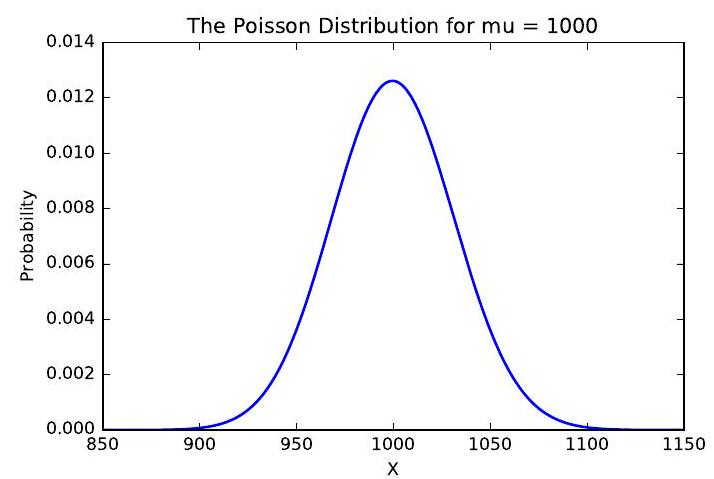
\includegraphics[max width=\textwidth]{2025_03_17_ca60ec0bfd96dcf8e028g-144}
\caption{The lifespan distribution of lightbulbs with an expected life of $\mu= 1000$ hours, as modeled by a Poisson distribution.}
\end{figure}

\begin{figure}[h]
\centering
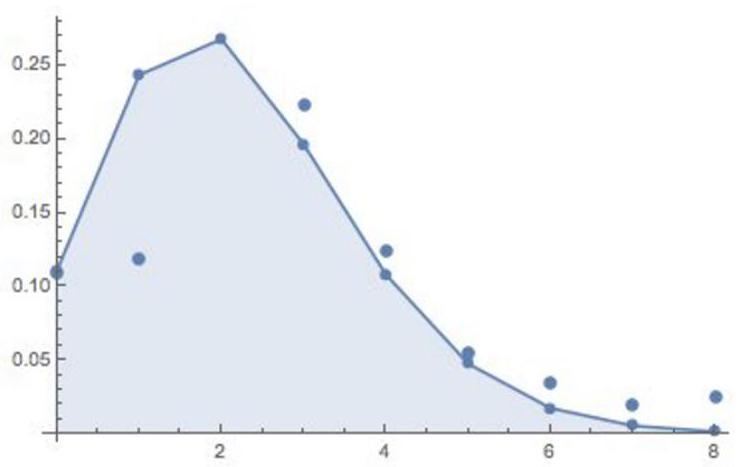
\includegraphics[max width=\textwidth]{2025_03_17_ca60ec0bfd96dcf8e028g-144(1)}
\caption{The observed fraction of families with $x$ kids (isolated points) is accurately modeled by Poisson distribution, defined by an average of $\mu=2.2$ children per family (polyline).}
\end{figure}

expect almost all bulbs to glow for between 900 and 1100 hours before the dying of the light.

Alternately, suppose we model the number of children by a process where the family keeps having children until after one too many tantrums, bake sales, or loads of laundry, a parent finally cracks. "That's it! I've had enough of this. No more!"

Under such a model, family size should be modeled as a Poisson distribution, where every day there is a small but non-zero probability of a breakdown that results in shutting down the factory.

How well does the "I've had it" model work to predict family size? The polygonal line in Figure 5.6 represents the Poisson distribution with the parameter $\lambda=2.2$, meaning families have an average of 2.2 kids. The points represent the fraction of families with $k$ children, drawn from the 2010 U.S. General Social\\
\begin{figure}[h]
\centering
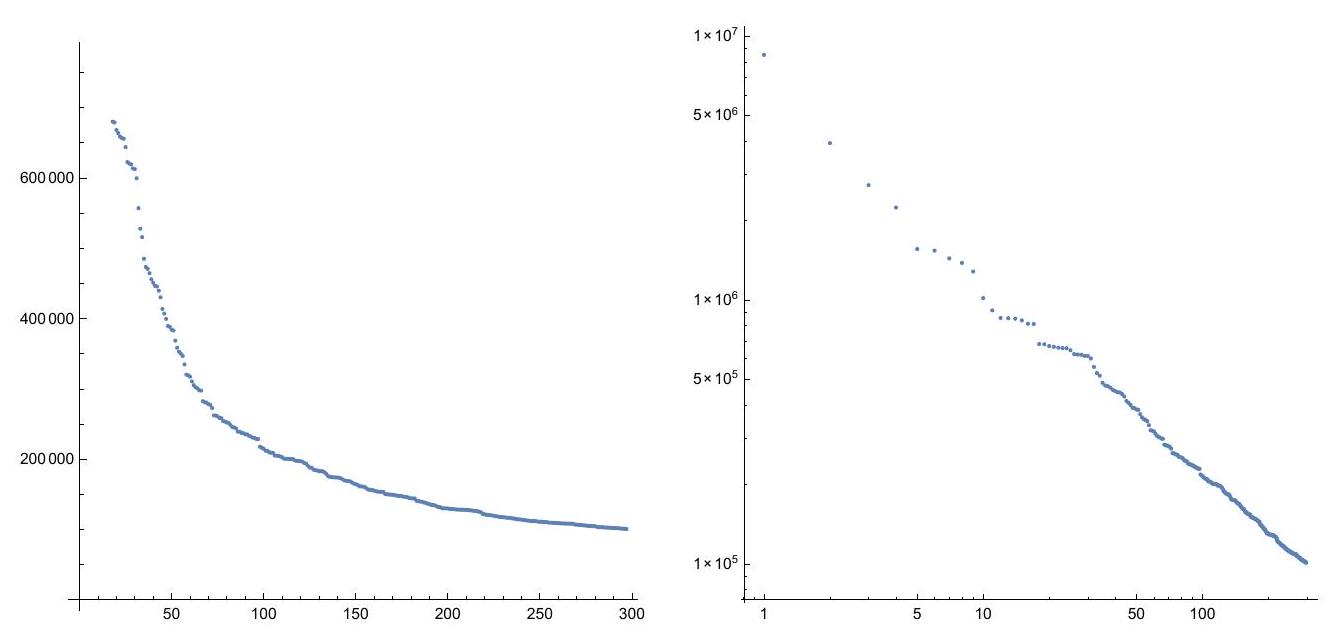
\includegraphics[max width=\textwidth]{2025_03_17_ca60ec0bfd96dcf8e028g-145}
\caption{The population of U.S. cities by decreasing rank (left). On the right is the same data, now including the very largest cities, but plotted on a log-log scale. That they sit on a line is indicative of a power law distribution.}
\end{figure}

Survey (GSS).\\
There is excellent agreement over all family sizes except $k=1$, and frankly, my personal experience suggests there are more singleton kids than this data set represents. Together, knowing just the mean and the formula for Poisson distribution enables us to construct a reasonable estimate of the real family-size distribution.

\subsection*{5.1.5 Power Law Distributions}
Many data distributions exhibit much longer tails than could be possible under the normal or Poisson distributions. Consider, for example, the population of cities. There were exactly 297 U.S. cities in 2014 with populations greater than 100,000 people, according to Wikipedia. The population of the $k$ th largest city, for $1 \leq k \leq 297$ is presented in Figure 5.7 (left). It shows that a relatively small number of cities have populations wildly dominating the rest. Indeed, the seventeen largest cities have populations so large they have been clipped off this plot so that we can see the rest.

These cities have a mean population of 304,689, with a ghastly standard deviation of 599,816. Something is wrong when the standard deviation is so large relative to the mean. Under a normal distribution, $99.7 \%$ of the mass lies within $3 \sigma$ of the mean, thus making it unlikely that any of these cities would have a population above 2.1 million people. Yet Houston has a population of 2.2 million people, and New York (at 8.4 million people) is more than $13 \sigma$ above the mean! City populations are clearly not normally distributed. In fact, they observe a different distribution, called a power law.

%---- Page End Break Here ---- Page : 129

For a given variable $X$ defined by a power law distribution,

\[
P(X=x)=c x^{-\alpha}
\]

This is parameterized by two constants: the exponent $\alpha$ and normalization constant $c$.

Power law distributions require some thinking to properly parse. The total probability defined by this distribution is the area under the curve:

\[
A=\int_{x=-\infty}^{\infty} c x^{-\alpha}=c \int_{x=-\infty}^{\infty} x^{-\alpha}
\]

The particular value of $A$ is defined by the parameters $\alpha$ and $c$. The normalization constant $c$ is chosen specifically for a given $\alpha$ to make sure that $A=1$, as demanded by the laws of probability. Other than that, $c$ is of no particular importance to us.

The real action happens with $\alpha$. Note that when we double the value of the input (from $x$ to $2 x$ ), we decrease the probability by a factor of $f=2^{-\alpha}$. This looks bad, but for any given $\alpha$ it is just a constant. So what the power law is really saying is that the probability of a $2 x$-sized event is $2^{\alpha}$ times less frequent than an $x$-sized event, for all $x$.

Personal wealth is well modeled by a power law, where $f \approx 0.2=1 / 5$. This means that over a large range, if $Z$ people have $x$ dollars, then $Z / 5$ people have $2 x$ dollars. One fifth as many people have $\$ 200,000$ than have $\$ 100,000$. If there are 625 people in the world worth $\$ 5$ billion, then there should be approximately 125 multi-billionaires each worth $\$ 10$ billion. Further, there should be 25 superbillionaires each worth $\$ 20$ billion, five hyper-billionaires at the $\$ 40$ billion level, and finally a single Bill Gates worth $\$ 80$ billion.

Power laws define the " $80 / 20$ " rules which account for all the inequality of our world: the observation that the top $20 \%$ of the $A$ gets fully $80 \%$ of the $B$. Power laws tend to arise whenever the rich get richer, where there is an increasing probability you will get more based on what you already have. Big cities grow disproportionately large because more people are attracted to cities when they are big. Because of his wealth, Bill Gates gets access to much better investment opportunities than I do, so his money grows faster than mine does.

Many distributions are defined by such preferential growth or attachment models, including:

\begin{itemize}
  \item \emph{Internet sites with $x$ users}: Websites get more popular because they have more users. You are more likely to join Instagram or Facebook because your friends have already joined Instagram or Facebook. Preferential attachment leads to a power law distribution.
  \item \emph{Words used with a relative frequency of $x$}: There is a long tail of millions of words like algorist or defenestrate$^{1}$ that are rarely used in the English
\end{itemize}

\footnotetext{${ }^{1}$ Defenestrate means "to throw someone out a window."
}
language. On the other hand, a small set of words like the are used wildly more often than the rest.

Zipf's law governs the distribution of word usage in natural languages, and states that the $k$ th most popular word (as measured by frequency rank) is used only $1 / k$ th as frequently as the most popular word. To gauge how well it works, consider the ranks of words based on frequencies from the English Wikipedia below:

\begin{center}
\begin{tabular}{c|c|c}
Rank & Word & Count \\
\hline
1 & the & 25131726 \\
110 & even & 415055 \\
212 & men & 177630 \\
312 & least & 132652 \\
412 & police & 99926 \\
514 & quite & 79205 \\
614 & include & 65764 \\
714 & knowledge & 57974 \\
816 & set & 50862 \\
916 & doctor & 46091 \\
\end{tabular}
\end{center}

\begin{center}
\begin{tabular}{c|c|c}
Rank & Word & Count \\
\hline
1017 & build & 41890 \\
2017 & essential & 21803 \\
3018 & sounds & 13867 \\
4018 & boards & 9811 \\
5018 & rage & 7385 \\
6019 & occupied & 5813 \\
7020 & continually & 4650 \\
8020 & delay & 3835 \\
9021 & delayed & 3233 \\
10021 & glances & 2767 \\
\end{tabular}
\end{center}

\begin{center}
\begin{tabular}{c|c|c}
Rank & Word & Count \\
\hline
10021 & glances & 2767 \\
20026 & ecclesiastical & 881 \\
30028 & zero-sum & 405 \\
40029 & excluded & 218 \\
50030 & sympathizes & 124 \\
60034 & capon & 77 \\
70023 & fibs & 49 \\
80039 & conventionalized & 33 \\
90079 & grandmom & 23 \\
100033 & slum-dwellers & 17 \\
\end{tabular}
\end{center}

It should be convincing that frequency of use drops rapidly with rank: recall that grandmom is only a slang form of grandma, not the real McCoy.

Why is this a power law? A word of rank $2 x$ has a frequency of $F_{2 x} \sim$ $F_{1} / 2 x$, compared to $F_{x} \sim F_{1} / x$. Thus halving the rank doubles the frequency, and this corresponds to the power law with $\alpha=1$.\\
What is the mechanism behind the evolution of languages that lead to this distribution? A plausible explanation is that people learn and use words because they hear other people using them. Any mechanism that favors the already popular leads to a power law.

\begin{itemize}
  \item \emph{Frequency of earthquakes of magnitude x}: The Richter scale for measuring the strength of earthquakes is logarithmic, meaning a 5.3 quake is ten times stronger than a 4.3 scale event. Adding one to the magnitude multiplies the strength by a factor of ten.\\
With such a rapidly increasing scale it makes sense that bigger events are rarer than smaller ones. I cause a 0.02 magnitude quake every time I flush a toilet. There are indeed billions of such events each day, but larger quakes get increasingly rare with size. Whenever a quantity grows in a potentially unbounded manner but the likelihood it does diminishes exponentially, you get a power law. Data shows this is as true of the energy released by earthquakes as it is with the casualties of wars: mercifully the number of conflicts which kill $x$ people decreases as a power law.
\end{itemize}

Learn to keep your eyes open for power law distributions. You will find them everywhere in our unjust world. They are revealed by the following properties:

\begin{itemize}
  \item \emph{Power laws show as straight lines on log value, log frequency plots:} Check out the graph of city populations in Figure 5.7(right). Although there are some gaps at the edges where data gets scarce, by and large the points lie\\
neatly on a line. This is the main characteristic of a power law. By the way, the slope of this line is determined by $\alpha$, the constant defining the shape of the power law distribution.
  \item \emph{The mean does not make sense}: Bill Gates alone adds about $\$ 250$ to the wealth of the average person in the United States. This is weird. Under a power law distribution there is a very small but non-zero probability that someone will have infinite wealth, so what does this do to the mean? The median does a much better job of capturing the bulk of such distributions than the observed mean.
  \item \emph{The standard deviation does not make sense}: In a power law distribution, the standard deviation is typically as large or larger than the mean. This means that the distribution is very poorly characterized by $\mu$ and $\sigma$, while the power law provides a very good description in terms of $\alpha$ and $c$.
  \item \emph{The distribution is scale invariant}: Suppose we plotted the populations of the 300th through 600th largest U.S. cities, instead of the top 300 as in Figure 5.7 (left). The shape would look very much the same, with the population of the 300th largest city towering over the tail. Any exponential function is scale invariant, because it looks the same at any resolution. This is a consequence of it being a straight line on a log-log plot: any subrange is a straight line segment, which has the same parameters in its window as the full distribution.
\end{itemize}

\subsection*{5.2 Sampling from Distributions}
Sampling points from a given probability distribution is a common operation, one which it is pays to know how to do. Perhaps you need test data from a power law distribution to run a simulation, or to verify that your program operates under extreme conditions. Testing whether your data in fact fits a particular distribution requires something to compare it against, and that should generally be properly-generated synthetic data drawn from the canonical distribution.

There is a general technique for sampling from any given probability distribution, called \emph{inverse transform sampling}. Recall that we can move between the probability density function $P$ and the cumulative density function $C$ by integration and differentiation. We can move back and forth between them because:

\[
P(k=X)=C^{\prime}(k)=C(X \leq k+\delta)-C(X \leq k), \text { and }
\]

\begin{figure}[h]
\centering
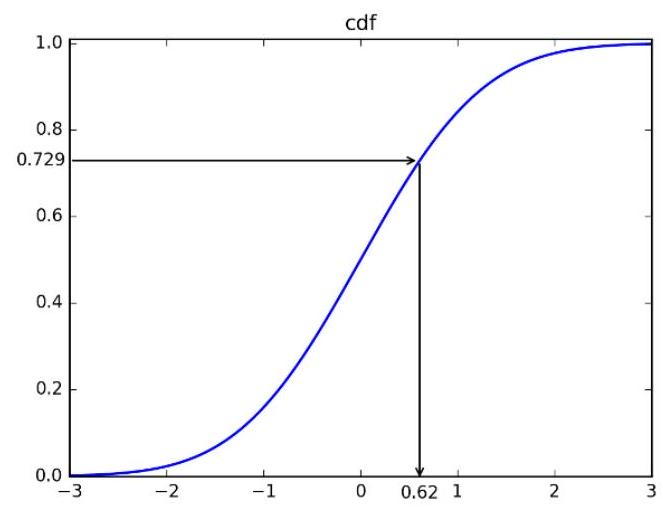
\includegraphics[max width=\textwidth]{2025_03_17_ca60ec0bfd96dcf8e028g-149}
\caption{The inverse transform sampling method enables us to convert a random number generated uniformly from $[0,1]$ (here 0.729 ) to a random sample drawn from any distribution, given its cdf.}
\end{figure}

\[
C(X \leq k)=\int_{x=-\infty}^{k} P(X=x)
\]

Suppose I want to sample a point from this possibly very complicated distribution. I can use a uniform random number generator to select a value $p$ in the interval $[0, \ldots, 1]$. We can interpret $p$ as a probability, and use it as an index on the cumulative distribution $C$. Precisely, we report the exact value of $x$ such that $C(X \leq x)=p$.

Figure 5.8 illustrates the approach, here sampling from the normal distribution. Suppose $p=0.729$ is the random number selected from our uniform generator. We return the $x$ value such that $y=0.729$, so $x=0.62$ as per this cdf.

If you are working with a popular probability distribution in a well-supported language like Python, there is almost certainly a library function to generate random samples already available. So look for the right library before you write your own.

\subsection*{5.2.1 Random Sampling beyond One Dimension}
Correctly sampling from a given distribution becomes a very subtle problem once you increase the number of dimensions. Consider the task of sampling points uniformly from within a circle. Think for a moment about how you might do this before we proceed.\
%---- Page End Break Here ---- Page : 133
\
\begin{figure}[h]
\centering
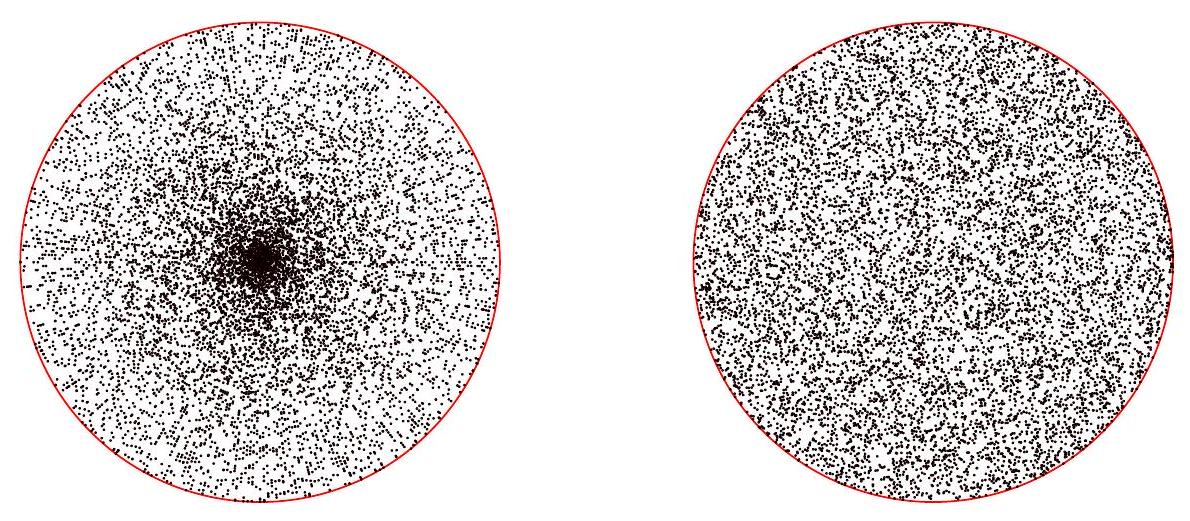
\includegraphics[max width=\textwidth]{2025_03_17_ca60ec0bfd96dcf8e028g-150}
\caption{Randomly generating 10,000 points by angle-radius pairs clearly oversamples near the origin of the circle (left). In contrast, Monte Carlo sampling generates points uniformly within the circle (right).}
\end{figure}

The clever among you may hit upon the idea of sampling the angle and distance from the center independently. The angle that any sampled point must make with respect to the origin and positive $x$-axis varies between 0 and $2 \pi$. The distance from the origin must be a value between 0 and $r$. Select these coordinates uniformly at random and you have a random point in the circle.

This method is clever, but wrong. Sure, any point so created must lie within the circle. But the points are not selected with uniform frequency. This method will generate points where half of them will lie within a distance of at most $r / 2$ from the center. But most of the area of the circle is farther from the center than that! Thus we will oversample near the origin, at the expense of the mass near the boundary. This is shown by Figure 5.9 (left), a plot of 10,000 points generated using this method.

A dumb technique that proves correct is Monte Carlo sampling. The $x$ and $y$ coordinates of every point in the circle range from $-r$ to $r$, as do many points outside the circle. Thus sampling these values uniformly at random gives us a point which lies in a bounding box of the circle, but not always within the circle itself. This can be easily tested: is the distance from $(x, y)$ to the origin at most $r$, i.e. is $\sqrt{x^{2}+y^{2}} \leq r$? If yes, we have found a random point in the circle. If not, we toss it out and try again. Figure 5.9 (right) plots 10,000 points constructed using this method: see how uniformly they cover the circle, without any obvious places of over- or under-sampling.

The efficiency here depends entirely upon the ratio of the desired region volume (the area of the circle) to the volume of the bounding box (the area of a square). Since $78.5 \%$ of this bounded box is occupied by the circle, less than two trials on average suffice to find each new circle point.

%---- Page End Break Here ---- Page : 134

Total revenue generated by arcades\\
correlates with\\
Computer science doctorates awarded in the US\\
\begin{figure}[h]
\centering
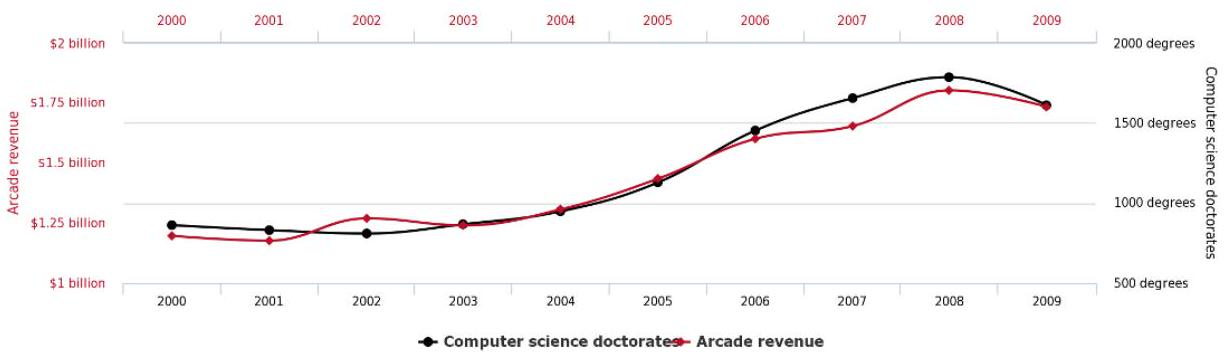
\includegraphics[max width=\textwidth]{2025_03_17_ca60ec0bfd96dcf8e028g-151}
\caption{Correlation vs. causation: the number of Computer Science Ph.Ds awarded each year in the United States strongly correlates with video/pinball arcade revenue. (from \cite{\cite{vigen2015spurious}})}
\end{figure}

\subsection*{5.3 Statistical Significance}
Statisticians are largely concerned with whether observations on data are \emph{significant}. Computational analysis will readily find a host of patterns and correlations in any interesting data set. But does a particular correlation reflect a real phenomena, as opposed to just chance? In other words, when is an observation really \emph{significant}?

Sufficiently strong correlations on large data sets may seem to be "obviously" meaningful, but the issues are often quite subtle. For one thing, \emph{correlation does not imply causation}. Figure 5.10 convincingly demonstrates that the volume of advanced study in computer science correlates with how much video games are being played. I'd like to think I have driven more people to algorithms than Nintendo, but maybe this is just the same thing? The graphs of such spurious correlations literally fill a book \cite{Vig15}, and a very funny one at that.

The discipline of statistics comes into its own in making subtle distinctions about whether an observation is meaningful or not. The classical example comes from medical statistics, in determining the efficacy of drug treatments. A pharmaceutical company conducts an experiment comparing two drugs. Drug $A$ cured 19 of 34 patients. Drug $B$ cured 14 of 21 patients. Is drug $B$ really better than drug $A$? FDA approval of new drugs can add or subtract billions from the value of drug companies. But can you be sure that a new drug represents a real improvement? How do you tell?

\subsection*{5.3.1 The Significance of Significance}
Statistical significance measures our confidence that there is a genuine difference between two given distributions. This is important. But statistical significance does not measure the importance or magnitude of this difference. For large
%---- Page End Break Here ---- Page : 135
```latex
\begin{figure}[h]
    \centering
    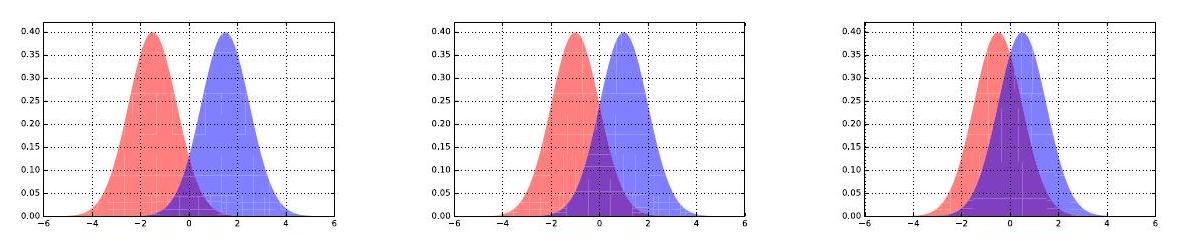
\includegraphics[max width=\textwidth]{2025_03_17_ca60ec0bfd96dcf8e028g-152}
    \caption{Pairs of normal distributions with the same variance, but decreasing difference in their means from left to right. As the means get closer, the greater overlap between the distributions makes it harder to tell them apart.}
    \label{fig:distributions-mean-difference}
\end{figure}

enough sample sizes, extremely small differences can register as highly significant on statistical tests.

For example, suppose I get suckered into betting tails on a coin which comes up heads 51\% of the time, instead of the 50\% we associate with a fair coin. After 100 tosses of a fair coin, I would expect to see 51\% or more heads 46.02\% of the time, so I have absolutely no grounds for complaint when I do. After 1,000 tosses, the probability of seeing at least 510 heads falls to 0.274. By 10,000 tosses, the probability of seeing so many heads is only 0.0233, and I should start to become suspicious of whether the coin is fair. After 100,000 tosses, the probability of fairness will be down to $1.29 \times 10^{-10}$, so small that I must issue a formal complaint, even if I thought my opponent to be a gentleman.

But here is the thing. Although it is now crystal clear that I had been tricked into using a biased coin, the consequences of this act are not substantial. For almost any issue in life worth flipping over, I would be willing to take the short side of the coin, because the stakes are just not high enough. At \$1 bet per flip, my expected loss even after 100,000 tosses would only be \$1,000 bucks.

Significance tells you how unlikely it is that something is due to chance, but not whether it is important. We really care about \textit{effect size}, the magnitude of difference between the two groups. We informally categorize a \textit{medium}-level effect size as visible to the naked eye by a careful observer. On this scale, \textit{large} effects pop out, and \textit{small} effects are not completely trivial \cite{\cite{sullivan2012effect}}. There are several statistics which try to measure the effect size, including:

\begin{itemize}
    \item \textit{Cohen's $d$}: The importance of the difference between two means $\mu$ and $\mu'$ depends on the absolute magnitude of the change, but also the natural variation of the distributions as measured by $\sigma$ or $\sigma'$. This effect size can be measured by:
\end{itemize}

\[
    d = \frac{|\mu - \mu'|}{\sigma}
\]

A reasonable threshold for a small effect size is $>0.2$, medium effect $>0.5$, and large effect size $>0.8$.

\begin{itemize}
    \item \textit{Pearson's correlation coefficient $r$}: Measures the degree of linear relationship between two variables, on a scale from $-1$ to $1$. The thresholds for effect sizes are comparable to the mean shift: small effects start at $\pm0.2$,
\end{itemize}
\begin{figure}[h]
    \centering
    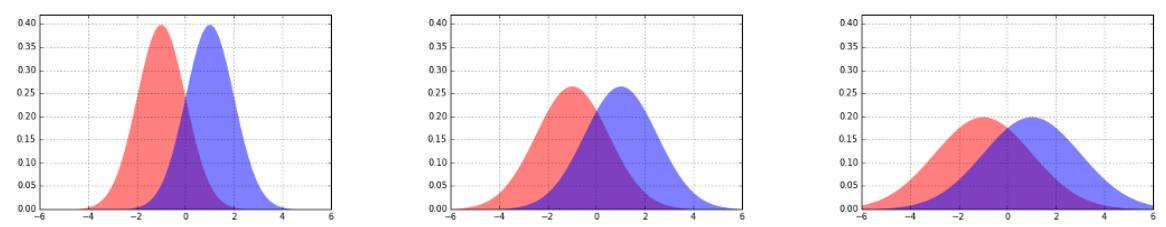
\includegraphics[max width=\textwidth]{2025_03_17_ca60ec0bfd96dcf8e028g-153}
    \caption{Pairs of normal distributions with the same difference in their means but increasing variance, from left to right. As the variance increases, there becomes greater overlap between the distributions, making it harder to tell them apart.}
    \label{fig:distributions-variance}
\end{figure}

medium effects about $\pm0.5$, and large effect sizes require correlations of $\pm0.8$.

\begin{itemize}
    \item \textit{The coefficient of variation $r^{2}$}: The square of the correlation coefficient reflects the proportion of the variance in one variable that is explained by the other. The thresholds follow from squaring those above. Small effects explain at least 4\% of the variance, medium effects $\geq 25\%$, and large effect sizes at least 64\%.
    \item \textit{Percentage of overlap}: The area under any single probability distribution is, by definition, 1. The area of intersection between two given distributions is a good measure of their similarity, as shown in Figure \ref{fig:distributions-mean-difference}. Identical distributions overlap 100\%, while disjoint intervals overlap 0\%. Reasonable thresholds are: for small effects 53\% overlap, medium effects 67\% overlap, and large effect sizes 85\% overlap.
\end{itemize}

Of course, any sizable effect which is not statistically significant is inherently suspect. The CS study vs. video game play correlation in Figure 5.10 was so high ($r=0.985$) that the effect size would be huge, were the number of sample points and methodology sound enough to support the conclusion.

\textit{Take-Home Lesson}: Statistical significance depends upon the number of samples, while the effect size does not.

\subsection{The T-test: Comparing Population Means}
We have seen that large mean shifts between two populations suggest large effect sizes. But how many measurements do we need before we can safely believe that the phenomenon is real? Suppose we measure the IQs of twenty men and twenty women. Does the data show that one group is smarter, on average? Certainly, the sample means will differ, at least a bit, but is this difference significant?

The t-test evaluates whether the population means of two samples are different. This problem commonly arises in \textit{A/B testing}, associated with evaluating whether a product change makes a difference in performance. Suppose you show one group of users version A, and another group version B. Further, suppose you measure a system performance value for each user, such as the number of times they click on ads or the number of stars they give when asked about the experience. The t-test measures whether the observed difference between the two groups is significant.

Two means differ significantly if:

\begin{itemize}
    \item \textit{The mean difference is relatively large}: This makes sense. One can conclude that men weigh more than women on average fairly easily, because the effect size is so large. According to the Center for Disease Control\footnote{\url{http://www.cdc.gov/nchs/fastats/obesity-overweight.htm}}, the average American male weighed 195.5 pounds in 2010, whereas the average American woman weighed 166.2 pounds. This is huge. Proving that a much more subtle difference, like IQ, is real requires much more evidence to be equally convincing.
    \item \textit{The standard deviations are small enough}: This also makes sense. It is easy to convince yourself that men and women have, on average, the same number of fingers because the counts we observe are very tightly bunched around the mean: $\{10, 10, 10, 10, 9, 10, \ldots\}$. The equal-finger count hypothesis would require much more evidence if the numbers jumped around a lot. I would be reluctant to commit to a true distributional average of $\mu=10$ if what I observed was $\{3, 15, 6, 14, 17, 5\}$.
    \item \textit{The number of samples are large enough}: This again makes sense. The more data I see, the more solidly I become convinced that the sample will accurately represent its underlying distribution. For example, men undoubtedly have \textit{fewer} fingers on average than women, as a consequence of more adventures with power tools\footnote{This observation alone may be sufficient to resolve the gender–IQ relationship, without the need for additional statistical evidence.}. But it would require a very large number of samples to observe and validate this relatively rare phenomenon.
\end{itemize}

The t-test starts by computing a \textit{test statistic} on the two sets of observations. Welch's t-statistic is defined as

\[
    t = \frac{\bar{x}_{1} - \bar{x}_{2}}{\sqrt{\frac{\sigma_{1}^{2}}{n_{1}} + \frac{\sigma_{2}^{2}}{n_{2}}}}
\]

where $\bar{x}_{i}, \sigma_{i}$, and $n_{i}$ are the mean, standard deviation, and population size of sample $i$, respectively.

Let us parse this equation carefully. The numerator is the difference between the means, so the bigger this difference, the bigger the value of the t-statistic. The standard deviations are in the denominator, so the smaller that $\sigma_{i}$ is, the bigger the value of the t-statistic. If this is confusing, recall what happens when you divide $x$ by a number approaching zero. Increasing the sample sizes $n_{i}$ also makes the denominator smaller, so the larger $n_{i}$ is, the bigger the value of the t-statistic. In all cases, the factors that make us more confident in there being a real difference between the two distributions increases the value of the t-statistic.

Interpreting the meaning of a particular value of the t-statistic comes from looking up a number in an appropriate table. For a desired \textit{significance level} $\alpha$ and number of \textit{degrees of freedom} (essentially the sample sizes), the table entry specifies the value $v$ that the t-statistic $t$ must exceed. If $t > v$, then the observation is significant to the $\alpha$ level.

\section*{Why Does This Work?}
Statistical tests like the t-test often seem like voodoo to me, because we look up a number from some magic table and treat it like gospel. \textit{The oracle has spoken: the difference is significant!} Of course, there is real mathematics behind significance testing, but the derivation involves calculus and strange functions (like the gamma function $\Gamma(n)$, a real numbered generalization of factorials). These complex calculations are why the convention arose to look things up in a precomputed table, instead of computing it yourself.

You can find derivations of the relevant formulae in any good statistics book, if you are interested. These tests are based on ideas like random sampling. We have seen how the mean and standard deviation constrain the shape of any underlying probability distribution. Getting a sample average very far from the mean implies bad luck. Randomly picking values several standard deviations away from the population mean is very unlikely, according to the theory. This makes it more likely that observing such a large difference is the result of drawing from a different distribution.

Much of the technicality here is a consequence of dealing with subtle phenomenon and small data sets. Historically, observed data was a very scarce resource, and it remains so in many situations. Recall our discussion of drug efficacy testing, where someone new must die for every single point we collect. The big data world you will likely inhabit generally features more observations (everybody visiting our webpage), lower stakes (do customers buy more when you show them a green background instead of a blue background?), and perhaps smaller effect sizes (how big an improvement do we really need to justify changing the background color?).
```
%---- Page End Break Here ---- Page : 147
```latex
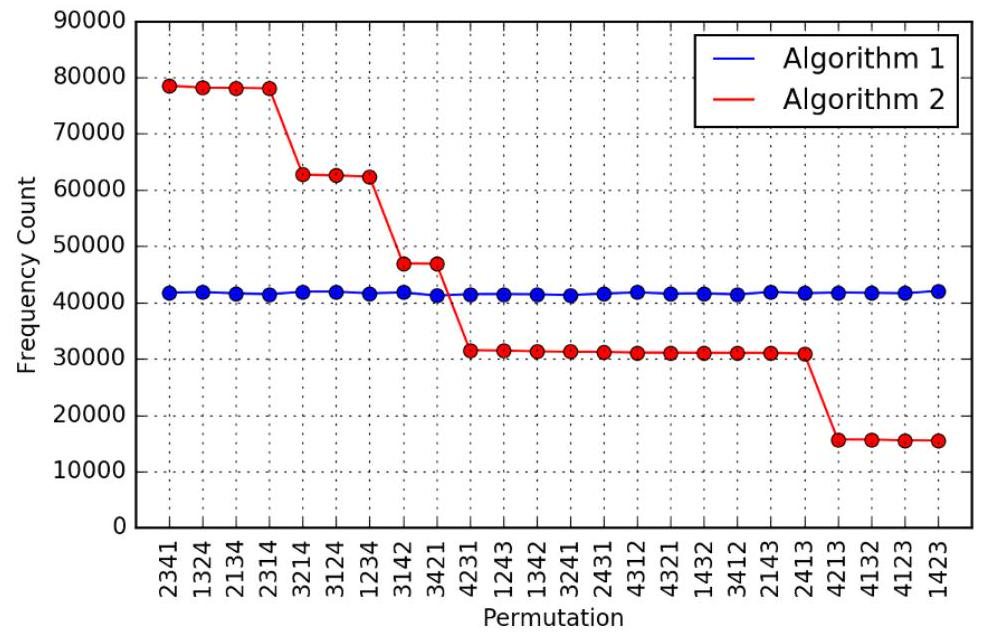
\includegraphics[max width=\textwidth, center]{2025_03_17_ca60ec0bfd96dcf8e028g-164}

\begin{figure}[H]
\centering
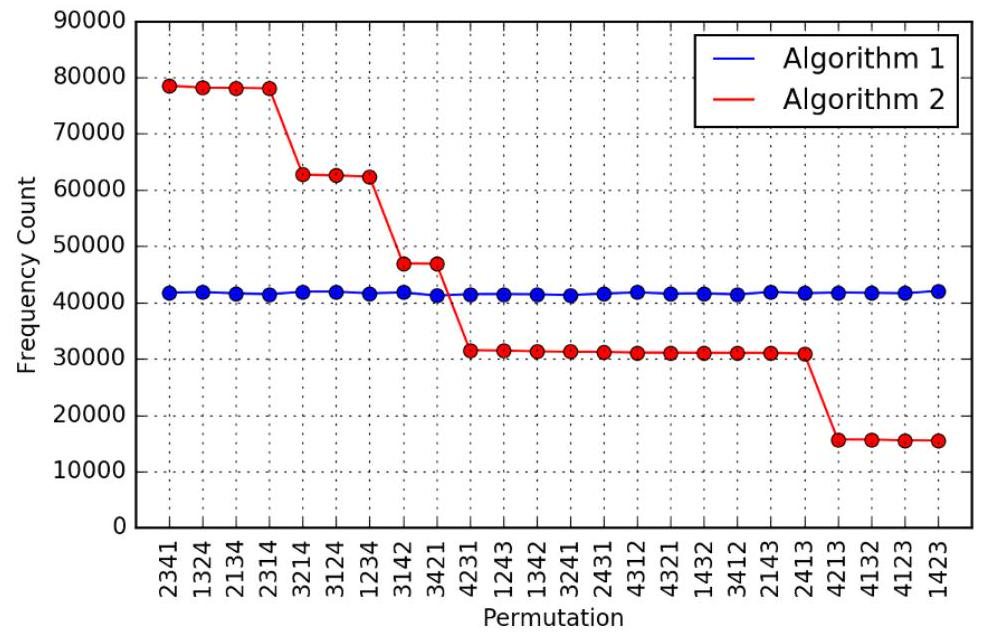
\includegraphics[max width=\textwidth]{2025_03_17_ca60ec0bfd96dcf8e028g-164}
\caption{The generation frequency of all $4!=24$ permutations using two different algorithms. Algorithm 1 generates them with uniform frequency, while algorithm 2 is substantially biased.}
\end{figure}

It recurs on the rest. It generates permutations uniformly at random. The second algorithm gives certain elements a better chance to end up first, showing that the distribution is not uniform.

But if you can't prove this theoretically, you can use the idea of a permutation test. Implement both of the algorithms, and perform 1,000,000 runs of each, constructing random permutations of, say, $n=4$ elements. Count how often each algorithm generates each one of the $4!=24$ distinct permutations. The results of such an experiment are shown in Figure \ref{fig:5.17}. Algorithm 1 proves incredibly steady, with a standard deviation of 166.1 occurrences. In contrast, there is an eight-fold difference between the most and least frequent permutations under algorithm 2, with $\sigma = 20,923.9$.

The moral here is that random generation can be very subtle. And that Monte Carlo-type experiments like permutation tests can eliminate the need for subtle reasoning. Verify, then trust.

\subsection{DiMaggio's Hitting Streak}
One of baseball's most amazing records is Joe DiMaggio's 56-game hitting streak. The job of a batter is to get hits, and they receive perhaps four chances every game to get one. Even very good hitters often fail.

But back in 1941, Joe DiMaggio succeeded in getting hits in 56 straight games, a truly amazing accomplishment. No player in the seventy-five years since then has come close to this record, nor any one before him.

But how unusual was such a long streak in the context of his career? DiMaggio played 1736 games, with 2214 hits in 6821 at bats. Thus he should get hits in roughly $1 - (1 - (2214 / 6821))^{4} = 79.2\%$ of his games with four at bats. What is the probability that someone with his skill level could manage such a consecutive game streak in the course of their career?

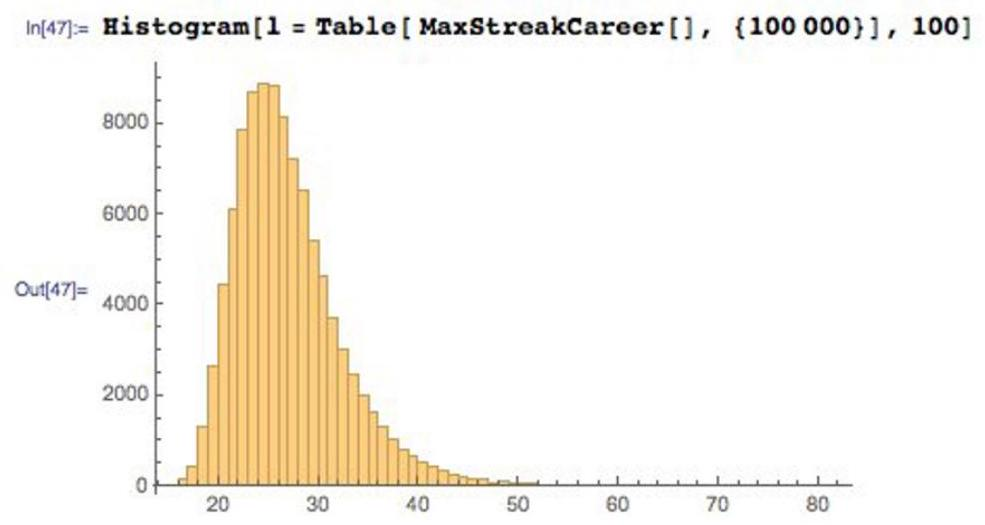
\includegraphics[max width=\textwidth, center]{2025_03_17_ca60ec0bfd96dcf8e028g-165}

\begin{figure}[H]
\centering
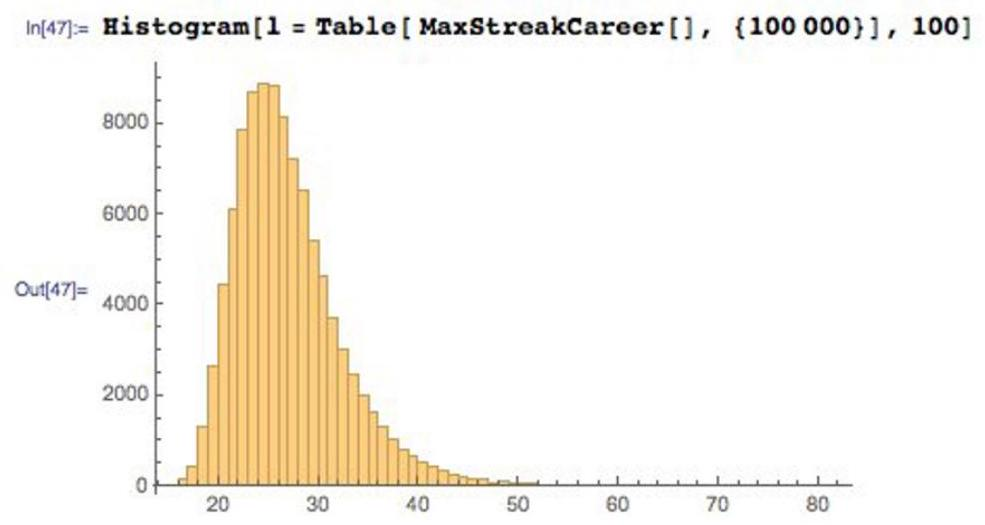
\includegraphics[max width=\textwidth]{2025_03_17_ca60ec0bfd96dcf8e028g-165}
\caption{The distribution of longest hitting streaks, over 100,000 simulated careers. DiMaggio's actual 56-game hitting streak stands at the very tail of this distribution, thus demonstrating the difficulty of this feat.}
\end{figure}

For those of you tired of my baseball analogies, let's put this in another context. Suppose you are a student who averages a grade of 90 on tests. You are a very good student to be sure, but not perfect. What are the chances you could have a hot streak where you scored above 90 on ten straight tests? What about twenty straight? Could you possibly ace 56 tests in a row?\footnote{Not if you are taking one of my classes, I tell you.} If such a long streak happened, would that mean that you had taken your studies to another level, or did you just get lucky?

So when DiMaggio had his hitting streak, was it just an expected consequence of his undisputed skills and consistency, or did he just get lucky? He was one of the very best hitters of his or any time, an all-star every season of his thirteen-year career. But we also know that DiMaggio got lucky from time to time. After all, he \textit{was} married to the movie star Marilyn Monroe.

To resolve this question, we used random numbers to simulate when he got hits over a synthetic "career" of 1736 games. Each game, the simulated Joe received four chances to hit and succeeded with a probability of $p = (2214 / 6821) = 0.325$. We could then identify the longest hitting streak over the course of this simulated career. By simulating 100,000 DiMaggio careers, we get a frequency distribution of streaks that can put the rarity of his accomplishment in context, getting a $p$-value in the process.

The results are shown in Figure \ref{fig:5.18}. In only 44 of 100,000 simulated careers ($p = 0.00044$) did DiMaggio manage a streak of at least 56 games. Thus, the length is quite out of line with what would be expected from him. The second longest streak of any major league hitter is only 44 games, so it is out of line with everyone else as well. But he also once hit in 61 straight games at a lower level of competition, so he seems to have had an extraordinary capacity for consistency.

Hitting streaks can be thought of as runs between games without hits, and so can be modeled using a Poisson distribution. But Monte Carlo simulations provide answers without detailed mathematics. Permutation tests give us insight with minimal knowledge and intellectual effort.

\subsection{Bayesian Reasoning}
The conditional probability $P(A \mid B)$ measures the likelihood of event $A$ given knowledge that event $B$ has occurred. We will rely on conditional probability throughout this book, because it lets us update our confidence in an event in response to fresh evidence, like observed data.

\textit{Bayes' Theorem} is an important tool for working with conditional probabilities, because it lets us turn the conditionals around:
\[
P(A \mid B) = \frac{P(B \mid A) P(A)}{P(B)}
\]

With Bayes theorem, we can convert the question of $P($outcome$\mid$data$)$ to $P($data $\mid$ outcome$)$, which is often much easier to compute. In some sense, Bayes’ theorem is just a consequence of algebra, but it leads to a different way of thinking about probability.

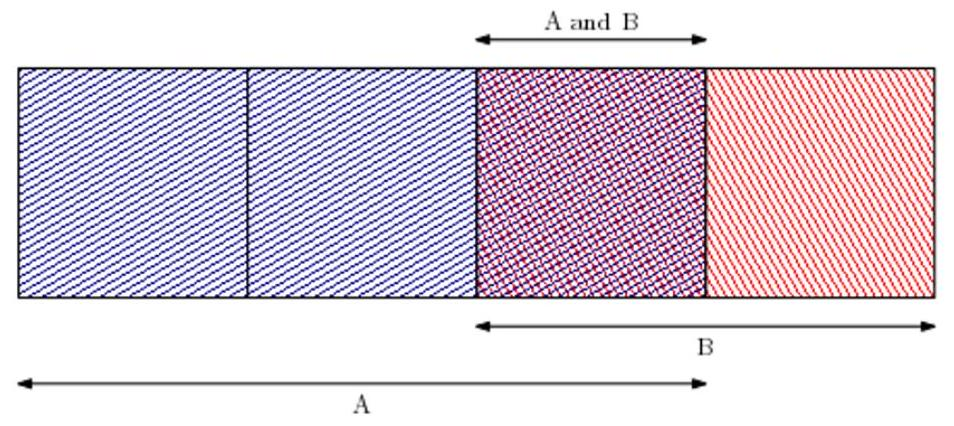
\includegraphics[max width=\textwidth, center]{2025_03_17_ca60ec0bfd96dcf8e028g-166}

\begin{figure}[H]
\centering
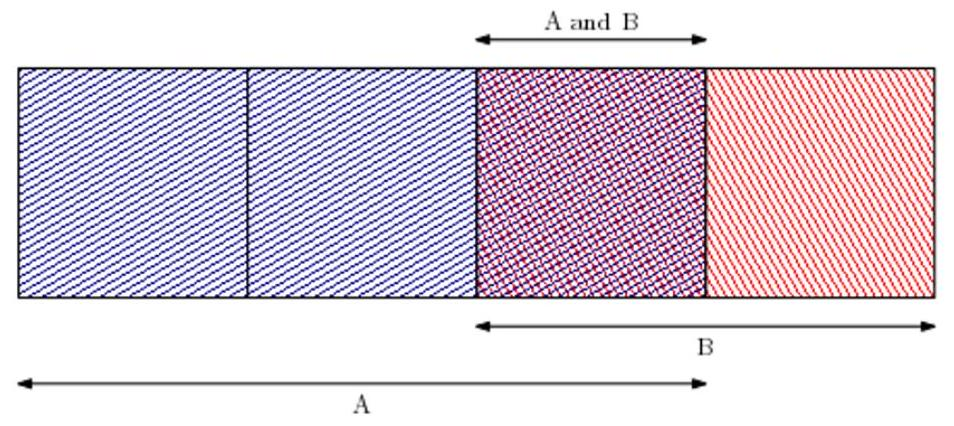
\includegraphics[max width=\textwidth]{2025_03_17_ca60ec0bfd96dcf8e028g-166}
\caption{Bayes' Theorem in action.}
\end{figure}

The event space consists of picking one of four blocks. The complex events $A$ and $B$ represent sub-ranges of blocks, where $P(A) = 3 / 4$ and $P(B) = 2 / 4 = 1/2$. By counting blocks from the figure, we can see that $P(A \mid B) = 1 / 2$ and $P(B \mid A) = 1 / 3$. These also follow directly from Bayes’ theorem:

\[
\begin{aligned}
P(A \mid B) &= \frac{P(B \mid A) P(A)}{P(B)} = \frac{(1 / 3) \cdot (3 / 4)}{(1 / 2)} = 1 / 2 \\
P(B \mid A) &= \frac{P(A \mid B) P(B)}{P(A)} = \frac{(1 / 2) \cdot (1 / 2)}{(3 / 4)} = 1 / 3
\end{aligned}
\]

Bayesian reasoning reflects how a prior probability $P(A)$ is updated to give the posterior probability $P(A \mid B)$ in the face of a new observation $B$, according to the ratio of the likelihood $P(B \mid A)$ and the marginal probability $P(B)$. The \textit{prior} probability $P(A)$ reflects our initial assumption about the world, to be revised based on the additional evidence $B$.

Bayesian reasoning is an important way to look at the world. Walking into Rachel and David’s wedding, my prior assumption was that the age distribution would reflect that of the world at large. But my confidence weakened with every elderly cousin I encountered, until it finally crumbled.

We will use Bayesian reasoning to build classifiers in Section 11.1. But keep this philosophy in mind as you analyze data. You should come to each task with a prior conception of what the answers should be, and then revise in accordance with statistical evidence.

\section{Chapter Notes}
Every data scientist should take a good elementary statistics course. Representative texts include Freedman \cite{\cite{freedman2007statistics}} and James et al. \cite{\cite{james2013introduction}}. Wheelan \cite{\cite{wheelan2013naked}} is a gentler introduction, with Huff \cite{\cite{huff2010how}} the classic treatise on how best to lie with statistics.

Donoho \cite{\cite{donoho2015data}} presents a fascinating history of data science from the vantage point of a statistician. It makes an effective case that most of the major principles of today’s data science were originally developed by statisticians, although they were not quickly embraced by the discipline at large. Modern statisticians have begun having much more satisfying conversations with computer scientists on these matters as interests have mutually converged.

Vigen \cite{Vig15} presents an amusing collection of spurious correlations drawn from a large number of interesting time series. Figure 5.10 is representative, and is reprinted with permission.

It has been demonstrated that the size of American families is reasonably well fit by a Poisson distribution. In fact, an analysis of household size distributions from 104 countries suggests that the “I’ve had enough” model works around the world \cite{\cite{jennings1999household}}.
```
%---- Page End Break Here ---- Page : 163
```latex
\subsection{Minimizing the Lie Factor}
A visualization seeks to tell a true story about what the data is saying. The baldest form of lie is to fudge your data, but it remains quite possible to report your data accurately, yet deliberately mislead your audience about what it is saying. Tufte defines the \emph{lie factor} of a chart as:
\[
\text{lie factor} = \frac{\text{(size of an effect in the graphic)}}{\text{(size of the effect in the data)}}
\]
Graphical integrity requires minimizing this lie factor, by avoiding the techniques which tend to mislead. Bad practices include:
\begin{itemize}
  \item \emph{Presenting means without variance}: The data values \{100, 100, 100, 100, 100\} and \{200, 0, 100, 200, 0\} tell different stories, even though both means are 100. If you cannot plot the actual points with the mean, at least show the variance, to make clear the degree to which the mean reflects the distribution.
  \item \emph{Presenting interpolations without the actual data}: Regression lines and fitted curves are effective at communicating trends and simplifying large data sets. But without showing the data points it is based on, it is impossible to ascertain the quality of the fit.
  \item \emph{Distortions of scale}: The aspect ratio of a figure can have a huge effect on how we interpret what we are seeing. Figure \ref{fig:financial-time-series} presents three renderings of a given financial time series, identical except for the aspect ratio of the chart.
\end{itemize}

In the bottom rendering, the series looks flat: there is nothing to worry about here. On the right, profits have fallen off a cliff: the sky is falling! The left corner plot presents a serious decline, but with signs of an autumn rebound.

Which plot is right? People are generally used to seeing plots presented according to the Golden ratio, implying that the width should be about 1.6 times the height. Give this shape to them, unless you have well-developed reasons why it is inappropriate. Psychologists inform us that 45 degree lines are the most readily interpretable, so avoid shapes that substantially amplify or mute lines from this objective.

\begin{figure}[h]
  \centering
  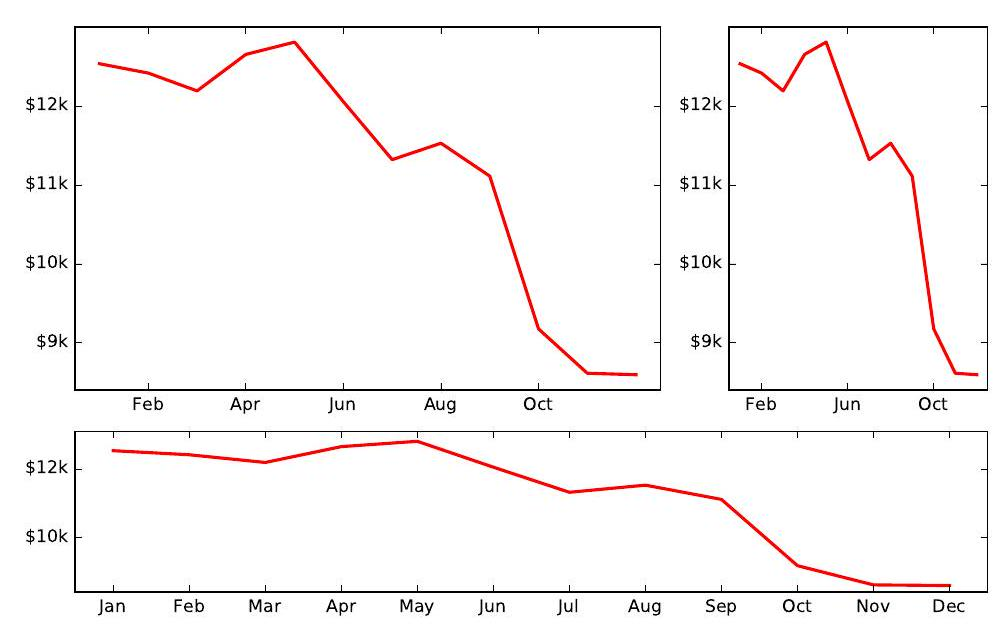
\includegraphics[max width=\textwidth]{2025_03_17_ca60ec0bfd96dcf8e028g-181}
  \caption{Three renderings of the same financial time series. Which most accurately represents the situation?}
  \label{fig:financial-time-series}
\end{figure}

\begin{itemize}
  \item \emph{Eliminating tick labels from numerical axes}: Even the worst scale distortions can be completely concealed by not printing numerical reference labels on axes. Only with the numerical scale markings can the actual data values be reconstructed from the plot.
  \item \emph{Hide the origin point from the plot}: The implicit assumption in most graphs is that the range of values on the $y$-axis goes from zero to $y_{\max}$. We lose the ability to visually compare magnitudes if the $y$-range instead goes from $y_{\min}-\epsilon$ to $y_{\max}$. The largest value suddenly looks many times larger than the smallest value, instead of being scaled to the proper proportion.
\end{itemize}

Despite Tufte's formula, the lie factor cannot be computed mechanically, because it requires understanding the agenda that is behind the distortion. In reading any graph, it is important to know who produced it and why. Understanding their agenda should sensitize you to potentially misleading messages encoded in the graphic.

\subsection{Minimizing Chartjunk}
Extraneous visual elements distract from the message the data is trying to tell. In an exciting graphic, the data tells the story, not the chartjunk.

\begin{figure}[h]
  \centering
  \includegraphics[max width=\textwidth]{2025_03_17_ca60ec0bfd96dcf8e028g-182}
  \caption{A monthly time series of sales. How can we improve/simplify this bar chart time series?}
\end{figure}

Figure \ref{fig:sales} presents a monthly time series of sales at a company beginning to encounter bad times. The graphic in question is a \emph{bar plot}, a perfectly sound way to represent time series data, and is drawn using conventional, perhaps default, options using a reasonable plotting package.

But can we simplify this plot by removing elements to make the data stand out better? Think about this for a minute before peeking at Figure \ref{fig:simplifications}, which presents a series of four successive simplifications to this chart. The critical operations are:

\begin{itemize}
  \item \emph{Jailbreak your data (upper left)}: Heavy grids imprison your data, by visually dominating the contents. Often graphs can be improved by removing the grid, or at least lightening it.
  \item \emph{Stop throwing shade (upper right)}: The colored background here contributes nothing to the interpretation of the graphic. Removing it increases the data-ink ratio, and makes it less obtrusive.
  \item \emph{Think outside the box (lower left)}: The bounding box does not really contribute information, particularly the upper and rightmost boundaries which do not define axes. Take them out, and let more air into your plots.
  \item \emph{Make missing ink work for you (lower right)}: The effect of the reference grid can be recovered by removing lines from the bars instead of adding elements. This makes it easier to compare the magnitude of biggest numbers, by focusing attention on big changes in the relatively small top piece, instead of small changes in the long bar.
\end{itemize}

\begin{figure}[h]
  \centering
  \includegraphics[max width=\textwidth]{2025_03_17_ca60ec0bfd96dcf8e028g-183}
  \caption{Four successive simplifications of Figure \ref{fig:sales} by removing extraneous non-data elements.}
  \label{fig:simplifications}
\end{figure}

The architect Mies van der Rohe famously said that "less is more." Removing elements from plots often improves them far more than adding things. Make this part of your graphical design philosophy.

\subsection{Proper Scaling and Labeling}
Deficiencies in scaling and labeling are the primary source of intentional or accidental misinformation in graphs. Labels need to report the proper magnitude of numbers, and scale needs to show these numbers to the right resolution, in a way to facilitate comparison. Generally speaking, data should be scaled so as to fill the space allotted to it on the chart.

Reasonable people can differ as to whether to scale the axes over the full theoretical range of the variable, or cut it down to reflect only the observed values. But certain decisions are clearly unreasonable.

\begin{figure}[h]
  \centering
  \includegraphics[max width=\textwidth]{2025_03_17_ca60ec0bfd96dcf8e028g-184}
  \caption{Scaling over the maximum possible range (left) is silly when all it shows is white space. Better scaling permits more meaningful comparisons (right).}
  \label{fig:scaling}
\end{figure}

The biggest sin of truncated scales comes when you do not show the whole of each bar, so the length of the bar no longer reflects the relative value of the variable. We show the $y=0$ line here, helping the reader to know that each bar must be whole. Getting the data out of its prison grid would also have helped.

\subsection{Effective Use of Color and Shading}
Colors are increasingly assumed as part of any graphical communication. Indeed, I was pleased to learn that my publisher's printing costs are now identical for color and black-and-white, so you the reader are not paying any more to see my color graphics here.

Colors play two major roles in charts, namely marking class distinctions and encoding numerical values. Representing points of different types, clusters, or classes with different colors encodes another layer of information on a conventional dot plot. This is a great idea when we are trying to establish the extent of differences in the data distribution across classes. The most critical thing is that the classes be easily distinguishable from each other, by using bold primary colors.

It is best when the colors are selected to have mnemonic values to link naturally to the class at hand. Losses should be printed in red ink, environmental causes associated with green, nations with their flag colors, and sports teams with their jersey colors. Coloring points to represent males as blue and females as red offers a subtle clue to help the viewer interpret a scatter plot, as shown in Figure 9.17.

Selecting colors to represent a numerical scale is a more difficult problem. Rainbow color maps are perceptually non-linear, meaning it is not obvious to anyone whether purple lies before or after green. Thus while plotting numbers in rainbow colors groups similar numbers in similar colors, the relative magnitudes are imperceptible without explicitly referencing the color scale. Figure \ref{fig:color-scales} presents several color scales from Python's MatPlotLib, for comparison.

\begin{figure}[h]
  \centering
  \includegraphics[max width=\textwidth]{2025_03_17_ca60ec0bfd96dcf8e028g-185}
  \caption{Color scales from Python's MatPlotLib, varying hue, saturation, and brightness. Rainbow color maps are perceptually non-linear, making it difficult to recognize the magnitudes of differences.}
  \label{fig:color-scales}
\end{figure}

Much better are color scales based on a varying either brightness or saturation. The \emph{brightness} of a color is modulated by blending the hue with a shade of gray, somewhere between white and black. \emph{Saturation} is controlled by mixing in a fraction of gray, where 0 produces the pure hue, and 1 removes all color.

As a general rule, large areas on plots should be shown with unsaturated colors. The converse is true for small regions, which stand out better with saturated colors. Color systems are a surprisingly technical and complicated matter, which means that you should always use well established color scales, instead of inventing your own.

\subsection{The Power of Repetition}
Small multiple plots and tables are excellent ways to represent multivariate data. Recall the power of grids showing all bivariate distributions in Figure 6.1.

There are many applications of small multiple charts. We can use them to break down a distribution by classes, perhaps plotting separate but comparable charts by region, gender, or time period. Arrays of plots facilitate comparisons: what has changed between different distributions.

Time series plots enable us to compare the same quantities at different calendar points. Even better is to compare multiple time series, either as lines on the same plot, or multiple plots in a logical array reflecting their relationship.

\subsection{Chart Types}
In this section, we will survey the rationale behind the primary types of data visualizations. For each chart, I present best practices for using them, and outline the degrees of freedom you have to make your presentation as effective as possible.

Nothing says "Here's a plot of some data" like a thoughtlessly-produced graphic, created using the default settings of some software tool. My students present me with such undigested data products way too often, and this section is somewhat of a personal reaction against it.

\emph{Take-Home Lesson}: You have the power and responsibility to produce meaningful and interpretable presentations of your work. Effective visualization involves an iterative process of looking at the data, deciding what story it is trying to tell, and then improving the display to tell the story better.

\begin{figure}[h]
  \centering
  \includegraphics[max width=\textwidth]{2025_03_17_ca60ec0bfd96dcf8e028g-187}
  \caption{A clever decision tree to help identify the best visual representation for representing data. Reprinted with permission from Abela [\cite{abela2013advanced}].}
\end{figure}

\subsection{Tabular Data}
Tables of numbers can be beautiful things, and are very effective ways to present data. Although they may \emph{appear} to lack the visual appeal of graphic presentations, tables have several advantages over other representations, including:
\begin{itemize}
  \item \emph{Representation of precision}: The resolution of a number tells you something about the process of how it was obtained: an average salary of \$79,815 says something different than \$80,000. Such subtleties are generally lost on plots, but nakedly clear in numerical tables.
  \item \emph{Representation of scale}: The digit lengths of numbers in a table can be likened to bar charts, on a logarithmic scale. Right-justifying numbers best communicates order-of-magnitude differences, as (to a lesser extent) does scanning the leading digits of numbers in a column.
\end{itemize}

\begin{center}
\begin{tabular}{lcr}
left & center & right \\
\hline
1 & 1 & 1 \\
10 & 10 & 10 \\
100 & 100 & 100 \\
1000 & 1000 & 1000 \\
\hline
\end{tabular}
\end{center}

Left justifying numbers prevents such comparisons, so always be sure to right justify them.

Presenting tabular data seems simple to do ("just put it in a table"), akin to rapping a leg with a stick. But subtleties go into producing the most informative tables. Best practices include:
\begin{itemize}
  \item \emph{Order rows to invite comparison}: You have the freedom to order the rows in a table any way you want, so take advantage of it. Sorting the rows according to the values of an important column is generally a good idea. Thus grouping the rows is valuable to facilitate comparison, by putting likes with likes.
  \item \emph{Order columns to highlight importance, or pairwise relationships}: Eyes darting from left-to-right across the page cannot make effective visual comparisons, but neighboring fields are easy to contrast. Generally speaking, columns should be organized to group similar fields, hiding the least important ones on the right.
  \item \emph{Right-justify uniform-precision numbers}: Visually comparing 3.1415 with 39.2 in a table is a hopeless task: the bigger number has to look bigger. Best is to right justify them, and set all to be the same precision: 3.14 vs. 39.20.
  \item \emph{Use emphasis, font, or color to highlight important entries}: Marking the extreme values in each column so they stand out reveals important information at a glance. It is easy to overdo this, however, so strive for subtlety.
  \item \emph{Avoid excessive-length column descriptors}: White ribbons in tables are distracting, and usually result from column labels that are longer than the values they represent. Use abbreviations or multiple-line word stacking to minimize the problem, and clarify any ambiguity in the caption attached to the table.
\end{itemize}

To help illustrate these possible sins, here is a table recording six properties of fifteen different nations, with the row and column orders given at random. Do you see any possible ways of improving it?

\begin{tabular}{l|llllll}
Country & Area & Density & Birthrate & Population & Mortality & GDP \\
\hline
Russia & 17075200 & 8.37 & 99.6 & 142893540 & 15.39 & 8900.0 \\
Mexico & 1972550 & 54.47 & 92.2 & 107449525 & 20.91 & 9000.0 \\
Japan & 377835 & 337.35 & 99.0 & 127463611 & 3.26 & 28200.0 \\
United Kingdom & 244820 & 247.57 & 99.0 & 60609153 & 5.16 & 27700.0 \\
New Zealand & 268680 & 15.17 & 99.0 & 4076140 & 5.85 & 21600.0 \\
Afghanistan & 647500 & 47.96 & 36.0 & 31056997 & 163.07 & 700.0 \\
Israel & 20770 & 305.83 & 95.4 & 6352117 & 7.03 & 19800.0 \\
United States & 9631420 & 30.99 & 97.0 & 298444215 & 6.5 & 37800.0 \\
China & 9596960 & 136.92 & 90.9 & 1313973713 & 24.18 & 5000.0 \\
Tajikistan & 143100 & 51.16 & 99.4 & 7320815 & 110.76 & 1000.0 \\
Burma & 678500 & 69.83 & 85.3 & 47382633 & 67.24 & 1800.0 \\
Tanzania & 945087 & 39.62 & 78.2 & 37445392 & 98.54 & 600.0 \\
Tonga & 748 & 153.33 & 98.5 & 114689 & 12.62 & 2200.0 \\
Germany & 357021 & 230.86 & 99.0 & 82422299 & 4.16 & 27600.0 \\
Australia & 7686850 & 2.64 & 100.0 & 20264082 & 4.69 & 29000.0 \\
\hline
\end{tabular}

There are many possible orderings of the rows (countries). Sorting by any single column is an improvement over random, although we could also group them by region/continent. The order of the columns can be made more understandable by putting like next to like. Finally, tricks like right-justifying numbers, removing uninformative digits, adding commas, and highlighting the biggest value in each column makes the data easier to read:

\begin{tabular}{l|rrrrrr}
 \multicolumn{7}{c}{\textbf{Birth}} \\
Country & Population & Area & Density & Mortality & GDP & \textbf{Rate} \\
\hline
Afghanistan & $31,056,997$ & 647,500 & 47.96 & \textbf{163.07} & 700 & 36.0 \\
Australia & $20,264,082$ & $7,686,850$ & 2.64 & 4.69 & 29,000 & \textbf{100.0} \\
Burma & $47,382,633$ & 678,500 & 69.83 & 67.24 & 1,800 & 85.3 \\
China & \textbf{1,313,973,713} & $9,596,960$ & 136.92 & 24.18 & 5,000 & 90.9 \\
Germany & $82,422,299$ & 357,021 & 230.86 & 4.16 & 27,600 & 99.0 \\
Israel & $6,352,117$ & 20,770 & 305.83 & 7.03 & 19,800 & 95.4 \\
Japan & $127,463,611$ & 377,835 & \textbf{337.35} & 3.26 & 28,200 & 99.0 \\
Mexico & $107,449,525$ & $1,972,550$ & 54.47 & 20.91 & 9,000 & 92.2 \\
New Zealand & $4,076,140$ & 268,680 & 15.17 & 5.85 & 21,600 & 99.0 \\
Russia & $142,893,540$ & \textbf{17,075,200} & 8.37 & 15.39 & 8,900 & 99.6 \\
Tajikistan & $7,320,815$ & 143,100 & 51.16 & 110.76 & 1,000 & 99.4 \\
Tanzania & $37,445,392$ & 945,087 & 39.62 & 98.54 & 600 & 78.2 \\
Tonga & 114,689 & 748 & 153.33 & 12.62 & 2,200 & 98.5 \\
United Kingdom & $60,609,153$ & 244,820 & 247.57 & 5.16 & 27,700 & 99.0 \\
United States & $298,444,215$ & $9,631,420$ & 30.99 & 6.50 & \textbf{37,800} & 97.0 \\
\hline
\end{tabular}

\begin{figure}[h]
  \centering
  \includegraphics[max width=\textwidth]{2025_03_17_ca60ec0bfd96dcf8e028g-190}
  \caption{Many of the line chart styles that we have seen are supported by Python's MatPlotLib package.}
\end{figure}

\subsection{Dot and Line Plots}
Dot and line plots are the most ubiquitous forms of data graphic, providing a visual representation of a function $\emph{y}=\emph{f}(x)$ defined by a set of $(x, y)$ points. Dot plots just show the data points, while line plots connect them or interpolate to define a continuous function $f(x)$. Figure \ref{fig:line-styles} shows several different styles of line plots, varying in the degree of emphasis they give the points vs. the interpolated curve. Advantages of line charts include:

\begin{itemize}
  \item \emph{Interpolation and fitting}: The interpolation curve derived from the points provides a prediction for $f(x)$ over the full range of possible $x$. This enables us to sanity check or reference other values, and make explicit the trends shown in the data.
  \item \emph{Dot plots}: A great thing about line plots is that you don’t actually have to show the line, resulting in a dot plot. Connecting points by line segments (polylines) proves misleading in many situations. If the function is only defined at integer points, or the $x$-values represent distinct conditions, then it makes no sense at all to interpolate between them.
\end{itemize}

Best practices with line charts include:

\begin{itemize}
  \item \emph{Show data points, not just fits}: It is generally important to show the actual data, instead of just the fitted or interpolated lines. The key is to make sure that one does not overwhelm the other. To represent large numbers of points unobtrusively, we can (a) reduce the size of the points, possibly to pinpricks, and/or (b) lighten the shade of the points so they sit in the background. Remember that there are fifty shades of gray, and that subtlety is the key.
  \item \emph{Show the full variable range if possible}: By default, most graphic software plots from $x_{\text {min}}$ to $x_{\text {max}}$ and $y_{\text {min}}$ to $y_{\max}$, where the mins and maxes are defined over the input data values. But the logical min and max are context specific, and it can reduce the lie factor to show the full range. Counts should logically start from zero, not $y_{\min}$. 
\end{itemize}
```
%---- Page End Break Here ---- Page : 180
```latex
\section{Chart Types}

\begin{figure}[h]
\centering
\includegraphics[max width=\textwidth]{2025_03_17_ca60ec0bfd96dcf8e028g-197}
\caption{Voter data from three U.S. presidential elections. Bar plots and pie charts display the frequency of proportion of categorical variables. Relative magnitudes in a time series can be displayed by modulating the area of the line or circle.}
\end{figure}

Figure~6.17 shows voter data from three years of U.S. presidential elections, presented as both pie and bar charts. The blue represents Democratic votes, the red Republican votes. The pies more clearly show which side won each election, but the bars show the Republican vote totals have stayed fairly constant while the Democrats were generally growing. Observe that these bars can be easily compared because they are left-justified.

Certain critics get whipped into an almost religious fever against pie charts, because they take up more space than necessary and are generally harder to read and compare. But pie charts are arguably better for showing percentages of totality. Many people seem to like them, so they are probably harmless in small quantities. Best practices for bar plots and pie charts include:

\begin{itemize}
  \item \textit{Directly label slices of the pie}: Pie charts are often accompanied by legend keys labeling what each color slice corresponds to. This is very distracting, because your eyes must move back and forth between the key and the pie to interpret this. Much better is to label each slice directly, inside the slice or just beyond the rim. This has a secondary benefit of discouraging the use of too many slices, because slivers generally become uninterpretable. It helps to group the slivers into a single slice called \textit{other}, and then perhaps present a second pie chart decomposed into the major \textit{other} components.
  \item \textit{Use bar charts to enable precise comparisons}: When anchored on a fixed line, arrays of bars make it easy to identify the minimum and maximum values in a series, and whether a trend is increasing or decreasing. Stacked bar charts are concise, but harder to use for such purposes. Presenting an array of small bar charts, here one for each gender/ethnic group, empowers us to make such fine comparisons, as shown in Figure~\ref{fig:small-multiples}.
  \item \textit{Scale appropriately, depending upon whether you seek to highlight absolute magnitude or proportion}: Pie charts exist to represent fractions of the whole. In presenting a series of pie or bar charts, your most critical decision is whether you want to show the size of the whole, or instead the fractions of each subgroup.
\end{itemize}

\begin{figure}[h]
\centering
\includegraphics[max width=\textwidth]{2025_03_17_ca60ec0bfd96dcf8e028g-198}
\caption{Small multiple bar plots/tables are excellent ways to represent multivariate data for comparison.}
\label{fig:small-multiples}
\end{figure}

\begin{figure}[h]
\centering
\includegraphics[max width=\textwidth]{2025_03_17_ca60ec0bfd96dcf8e028g-198(1)}
\includegraphics[max width=\textwidth]{2025_03_17_ca60ec0bfd96dcf8e028g-199}
\caption{Stacked bar charts illustrating the survivorship rate on the doomed ship Titanic, by ticket class. The histogram (left) informs us of the size of each class, but scaled bars (right) better capture proportions. Primary conclusion: you were better off not to be traveling steerage (third class).}
\end{figure}

Figure~6.19 shows two stacked bar charts presenting survivorship statistics on the doomed ship \textit{Titanic}, reported by ticket class. The histogram (left) precisely records the sizes of each class and the resulting outcomes. The chart with equal length bars (right) better captures how the mortality rate increased for lower classes. Pie charts can also be used to show changes in magnitude, by varying the area of the circle defining the pie. But it is harder for the eye to calculate area than length, making comparisons difficult. Modulating the radius to reflect magnitude instead of area is even more deceptive, because doubling the radius of a circle multiplies the area by four.

\subsection*{Bad Pie Charts}

\begin{figure}[h]
\centering
\includegraphics[max width=\textwidth]{2025_03_17_ca60ec0bfd96dcf8e028g-199}
\caption{Pie charts of delegates to the 2016 Republican convention by candidate. Which one is better and why?}
\end{figure}

Figure~6.20 shows two pie charts reporting the distribution of delegates to the 2016 Republican convention, by candidate. The left pie is two-dimensional, while the chart on right has thick slices neatly separated to show off this depth. Which one is better at conveying the distribution of votes?

It should be clear that the three-dimensional effects and separation are pure chartjunk, that only obscures the relationship between the size of the slices. The actual data values disappeared as well, perhaps because there wasn't enough space left for them after all those shadows. But why do we need a pie chart at all? A little table of labels/colors with an extra column with percentages would be more concise and informative.

\subsection{Histograms}

The interesting properties of variables or features are defined by their underlying frequency distribution. Where is the peak of the distribution, and is the mode near the mean? Is the distribution symmetric or skewed? Where are the tails? Might it be bimodal, suggesting that the distribution is drawn from a mix of two or more underlying populations?

\begin{figure}[h]
\centering
\includegraphics[max width=\textwidth]{2025_03_17_ca60ec0bfd96dcf8e028g-200}
\caption{Time series of vote totals in U.S. presidential elections by party enable us to see the changes in magnitude and distribution. Democrats are shown in blue, and Republicans in red. It is hard to visualize changes, particularly in the middle layers of the stack.}
\end{figure}

Often we are faced with a large number of observations of a particular variable, and seek to plot a representation for them. Histograms are plots of the observed frequency distributions. When the variable is defined over a large range of possible values relative to the $n$ observations, it is unlikely we will ever see any exact duplication. However, by partitioning the value range into an appropriate number of equal-width bins, we can accumulate different counts per bin, and approximate the underlying probability distribution.

The biggest issue in building a histogram is deciding on the right number of bins to use. Too many bins, and there will be only a few points in even the most popular bucket. We turned to binning to solve exactly this problem in the first place. But use too few bins, and you won't see enough detail to understand the shape of the distribution.

Figure~6.22 illustrates the consequences of bin size on the appearance of a histogram. The plots in the top row bin 100,000 points from a normal distribution into ten, twenty, and fifty buckets respectively. There are enough points to fill fifty buckets, and the distribution on right looks beautiful. The plots in the bottom row bin have only 100 points, so the thirty-bucket plot on right is sparse and scraggy. Here seven bins (shown on the left) seems to produce the most representative plot.

It is impossible to give hard and fast rules to select the best bin count $b$ for showing off your data. Realize you will never be able to discriminate between more than a hundred bins by eye, so this provides a logical upper bound. In general, I like to see an average of 10 to 50 points per bin to make things smooth, so $b = \lceil n / 25 \rceil$ gives a reasonable first guess. But experiment with different values of $b$, because the right bin count will work much better than the others. You will know it when you see it.

\begin{figure}[h]
\centering
\includegraphics[max width=\textwidth]{2025_03_17_ca60ec0bfd96dcf8e028g-201}
\caption{Histograms of a given distribution can look wildly different depending on the number of bins. A large data set benefits from many bins (top). But the structure of a smaller data set is best shown when each bin a non-trivial number of elements.}
\end{figure}

\begin{figure}[h]
\centering
\includegraphics[max width=\textwidth]{2025_03_17_ca60ec0bfd96dcf8e028g-202(1)}
\caption{Dividing counts by the total yields a probability density plot, which is more generally interpretable even though the shapes are identical.}
\end{figure}

\begin{figure}[h]
\centering
\includegraphics[max width=\textwidth]{2025_03_17_ca60ec0bfd96dcf8e028g-202}
\caption{Generally speaking, histograms are better for displaying peaks in a distribution, but cdfs are better for showing tails.}
\end{figure}

Best practices for histograms include:

\begin{itemize}
  \item \textit{Turn your histogram into a pdf}: Typically, we interpret our data as observations that approximate the probability density function (pdf) of an underlying random variable. If so, it becomes more interpretable to label the $y$-axis by the fraction of elements in each bucket, instead of the total count. This is particularly true in large data sets, where the buckets are full enough that we are unconcerned about the exact level of support. Figure~6.23 shows the same data, plotted on the right as a pdf instead of a histogram. The shape is exactly the same in both plots: all that changes is the label on the $y$-axis. Yet the result is easier to interpret, because it is in terms of probabilities instead of counts.
  \item \textit{Consider the cdf}: The cumulative density function (cdf) is the integral of the pdf, and the two functions contain exactly the same information. So consider using a cdf instead of a histogram to represent your distribution, as shown in Figure~6.24. One great thing about plotting the cdf is that it does not rely on a bin count parameter, so it presents a true, unadulterated view of your data. Recall how great the cdfs looked in the Kolmogorov-Smirnov test, Figure~5.13. We draw a cdf as a line plot with $n+2$ points for $n$ observations. The first and last points are $(x_{\min} - \epsilon, 0)$ and $(x_{\max} + \epsilon, 1)$. We then sort the observations to yield $S = \{s_{1}, \ldots, s_{n}\}$, and plot $(s_{i}, i/n)$ for all $i$.

Cumulative distributions require slightly more sophistication to read than histograms. The cdf is monotonically increasing, so there are no peaks in the distribution. Instead, the mode is marked by the longest vertical line segment. But cdfs are much better at highlighting the tails of a distribution. The reason is clear: the small counts at the tails are obscured by the axis on a histogram, but accumulate into visible stuff in the cdf.
\end{itemize}
```

%---- Page End Break Here ---- Page : 202
```
\subsection{Philosophies of Modeling}

I associate the word \textit{bias} with prejudice, and the correspondence is fairly apt: an apriori assumption that one group is inferior to another will result in less accurate predictions than an unbiased one. Models that perform lousy on both training and testing data are underfit.

Errors of variance result in \textit{overfit} models: their quest for accuracy causes them to mistake noise for signal, and they adjust so well to the training data that noise leads them astray. Models that do much better on testing data than training data are overfit\footnote{To complete this taxonomy, models that do better on testing data than the training data are said to be cheating.}

Take-Home Lesson: \textit{Models based on first principles or assumptions are likely to suffer from bias, while data-driven models are in greater danger of overfitting.}

\subsubsection{What Would Nate Silver Do?}

Nate Silver is perhaps the most prominent public face of data science today. A quantitative fellow who left a management consulting job to develop baseball forecasting methods, he rose to fame through his election forecast website \url{http://www.fivethirtyeight.com}. Here he used quantitative methods to analyze poll results to predict the results of U.S. presidential elections. In the 2008 election, he accurately called the winner of 49 of the 50 states, and improved in 2012 to bag 50 out of 50. The results of the 2016 election proved a shock to just about everyone, but alone among public commentators Nate Silver had identified a substantial chance of Trump winning the electoral college while losing the popular vote. This indeed proved to be the case.

Silver wrote an excellent book \textit{The Signal and the Noise: Why so many predictions fail – but some don’t} \cite{Sil12}. There he writes sensibly about state-of-the-art forecasting in several fields, including sports, weather and earthquake prediction, and financial modeling. He outlines principles for effective modeling, including:

\begin{itemize}
  \item \textit{Think probabilistically}: Forecasts which make concrete statements are \textit{less} meaningful than those that are inherently probabilistic. A forecast that Trump has only 28.3\% chance of winning is more meaningful than one that categorically states that he will lose.
\end{itemize}

The real world is an uncertain place, and successful models recognize this uncertainty. There are always a range of possible outcomes that can occur with slight perturbations of reality, and this should be captured in your model. Forecasts of numerical quantities should not be single numbers, but instead report probability distributions. Specifying a standard deviation, \(\sigma\), along with the mean prediction, \(\mu\), suffices to describe such a distribution, particularly if it is assumed to be normal.

Several of the machine learning techniques we will study naturally provide probabilistic answers. Logistic regression provides a confidence along with each classification it makes. Methods that vote among the labels of the \(k\) nearest neighbors define a natural confidence measure, based on the consistency of the labels in the neighborhood. Collecting ten of eleven votes for blue means something stronger than seven out of eleven.

\begin{itemize}
  \item \textit{Change your forecast in response to new information}: Live models are much more interesting than dead ones. A model is \textit{live} if it is continually updating predictions in response to new information. Building an infrastructure that maintains a live model is more intricate than that of a one-off computation, but much more valuable.
  
  Live models are more intellectually honest than dead ones. \textit{Fresh information should} change the result of any forecast. Scientists should be open to changing opinions in response to new data: indeed, this is what separates scientists from hacks and trolls.
\end{itemize}

Dynamically-changing forecasts provide excellent opportunities to evaluate your model. Do they ultimately converge on the correct answer? Does uncertainty diminish as the event approaches? Any live model should track and display its predictions over time, so the viewer can gauge whether changes accurately reflected the impact of new information.

\begin{itemize}
  \item \textit{Look for consensus}: A good forecast comes from multiple distinct sources of evidence. Data should derive from as many different sources as possible. Ideally, multiple models should be built, each trying to predict the same thing in different ways. You should have an opinion as to which model is the best, but be concerned when it substantially differs from the herd.
  
  Often third parties produce competing forecasts, which you can monitor and compare against. Being different doesn’t mean that you are wrong, but it does provide a reality check. Who has been doing better lately? What explains the differences in the forecast? Can your model be improved?
  
  Google’s Flu Trends forecasting model predicted disease outbreaks by monitoring key words on search: a surge in people looking for \textit{aspirin} or \textit{fever} might suggest that illness is spreading. Google’s forecasting model proved quite consistent with the Center for Disease Control’s (CDC) statistics on actual flu cases for several years, until they embarrassingly went astray.
  
  The world changes. Among the changes was that Google’s search interface began to suggest search queries in response to a user’s history. When offered the suggestion, many more people started searching for \textit{aspirin} after searching for \textit{fever}. And the old model suddenly wasn’t accurate anymore. Google’s sins lay in not monitoring its performance and adjusting over time.
\end{itemize}

Certain machine learning methods explicitly strive for consensus. \textit{Boosting} algorithms combine large numbers of weak classifiers to produce a strong one. Ensemble decision tree methods build many independent classifiers, and vote among them to make the best decision. Such methods can have a robustness which eludes more single-track models.

\begin{itemize}
  \item \textit{Employ Baysian reasoning}: Bayes’ theorem has several interpretations, but perhaps most cogently provides a way to calculate how probabilities change in response to new evidence. When stated as
\end{itemize}

\[ 
P(A \mid B)=\frac{P(B \mid A) P(A)}{P(B)} 
\]

it provides a way to calculate how the probability of event \(A\) changes in response to new evidence \(B\).

Applying Bayes’ theorem requires a \textit{prior} probability \(P(A)\), the likelihood of event \(A\) \textit{before} knowing the status of a particular event \(B\). This might be the result of running a classifier to predict the status of \(A\) from other features, or background knowledge about event frequencies in a population. Without a good estimate for this prior, it is very difficult to know how seriously to take the classifier.

Suppose \(A\) is the event that person \(x\) is actually a terrorist, and \(B\) is the result of a feature-based classifier that decides if \(x\) looks like a terrorist. When trained/evaluated on a data set of 1,000 people, half of whom were terrorists, the classifier achieved an enviable accuracy of, say, 90\%. The classifier now says that Skiena looks like a terrorist. What is the probability that Skiena \textit{really} is a terrorist?

The key insight here is that the prior probability of “\(x\) is a terrorist” is really, really low. If there are a hundred terrorists operating in the United States, then \(P(A)=100/300,000,000=3.33\times 10^{-7}\). The probability of the terrorist detector saying yes, \(P(B)=0.5\), while the probability of the detector being right when it says yes \(P(B \mid A)=0.9\). Multiplying this out gives a still very tiny probability that I am a bad guy,

\[
P(A \mid B)=\frac{P(B \mid A) P(A)}{P(B)}=\frac{(0.9)(3.33 \times 10^{-7})}{(0.5)}=6 \times 10^{-7}
\]

although admittedly now greater than that of a random citizen.

Factoring in prior probabilities is essential to getting the right interpretation from this classifier. Bayesian reasoning starts from the prior distribution, then weighs further evidence by how strongly it should impact the probability of the event.

\section{A Taxonomy of Models}

Models come in, well, many different models. Part of developing a philosophy of modeling is understanding your available degrees of freedom in design and implementation. In this section, we will look at model types along several different dimensions, reviewing the primary technical issues which arise to distinguish each class.

\subsection{Linear vs. Non-Linear Models}

Linear models are governed by equations that weigh each feature variable by a coefficient reflecting its importance, and sum up these values to produce a score. Powerful machine learning techniques, such as linear regression, can be used to identify the best possible coefficients to fit training data, yielding very effective models.

But generally speaking, the world is not linear. Richer mathematical descriptions include higher-order polynomials, logarithms, and exponentials. These permit models that fit training data much more tightly than linear functions can. Generally speaking, it is much harder to find the best possible coefficients to fit non-linear models. But we don’t \textit{have} to find the best possible fit: deep learning methods, based on neural networks, offer excellent performance despite inherent difficulties in optimization.

Modeling cowboys often sneer in contempt at the simplicity of linear models. But linear models offer substantial benefits. They are readily understandable, generally defensible, easy to build, and avoid overfitting on modest-sized data sets. Occam’s razor tells us that “the simplest explanation is the best explanation.” I am generally happier with a robust linear model, yielding an accuracy of \(x\%\), than a complex non-linear beast only a few percentage points better on limited testing data.

\subsection{Blackbox vs. Descriptive Models}

Black boxes are devices that do their job, but in some unknown manner. Stuff goes in and stuff comes out, but how the sausage is made is completely impenetrable to outsiders.

By contrast, we prefer models that are \textit{descriptive}, meaning they provide some insight into why they are making their decisions. Theory-driven models are generally descriptive, because they are explicit implementations of a particular well-developed theory. If you believe the theory, you have a reason to trust the underlying model, and any resulting predictions.

Certain machine learning models prove less opaque than others. Linear regression models are descriptive, because one can see exactly which variables receive the most weight, and measure how much they contribute to the resulting prediction. Decision tree models enable you to follow the exact decision path used to make a classification. “Our model denied you a home mortgage because your income is less than \$10,000 per year, you have greater than \$50,000 in credit card debt, and you have been unemployed over the past year.”

But the unfortunate truth is that blackbox modeling techniques such as deep learning can be extremely effective. Neural network models are generally completely opaque as to \textit{why} they do what they do. Figure 7.1 makes this clear. It shows images which were very carefully constructed to fool state-of-the-art neural networks. They succeeded brilliantly. The networks in question had \(\geq 99.6\%\) confidence that they had found the right label for every image in Figure 7.1.

\begin{figure}[h]
\centering
\includegraphics[max width=\textwidth]{2025_03_17_ca60ec0bfd96dcf8e028g-223}
\caption{Synthetic images that are mistakenly recognized as objects by state-of-the-art Deep Learning neural networks, each with a confidence greater than 99.6\%. Source: \cite{nguyen2015deep}.}
\end{figure}

The scandal here is not that the network got the labels wrong on these perverse images, for these recognizers are very impressive systems. Indeed, they were much more accurate than dreamed possible only a year or two before. The problem is that the creators of these classifiers had no idea why their programs made such terrible errors, or how they could prevent them in the future.

A similar story is told of a system built for the military to distinguish images of cars from trucks. It performed well in training, but disastrously in the field. Only later was it realized that the training images for cars were shot on a sunny day and those of trucks on a cloudy day, so the system had learned to link the sky in the background with the class of the vehicle.

Tales like these highlight why visualizing the training data and using descriptive models can be so important. You must be convinced that your model has the information it needs to make the decisions you are asking of it, particularly in situations where the stakes are high.

\subsection{First-Principle vs. Data-Driven Models}

\textit{First-principle models} are based on a belief of how the system under investigation really works. It might be a theoretical explanation, like Newton’s laws of motion. Such models can employ the full weight of classical mathematics: calculus, algebra, geometry, and more. The model might be a discrete event simulation, as will be discussed in Section 7.7. It might be seat-of-the-pants reasoning from an understanding of the domain: voters are unhappy if the economy is bad, therefore variables which measure the state of the economy should help us predict who will win the election.

In contrast, \textit{data-driven models} are based on observed correlations between input parameters and outcome variables. The same basic model might be used to predict tomorrow’s weather or the price of a given stock, differing only on the data it was trained on. Machine learning methods make it possible to build an effective model on a domain one knows nothing about, provided we are given a good enough training set.

Because this is a book on data science, you might infer that my heart lies more on the side of data-driven models. But this isn’t really true. Data science is also about \textit{science}, and things that happen for understandable reasons. Models which ignore this are doomed to fail embarrassingly in certain circumstances.

There is an alternate way to frame this discussion, however. \textit{Ad hoc models} are built using domain-specific knowledge to guide their structure and design. These tend to be brittle in response to changing conditions, and difficult to apply to new tasks. In contrast, machine learning models for classification and regression are \textit{general}, because they employ no problem-specific ideas, only specific data. Retrain the models on fresh data, and they adapt to changing conditions. Train them on a different data set, and they can do something completely different. By this rubric, general models sound much better than ad hoc ones.

The truth is that the best models are a mixture of both theory and data. It is important to understand your domain as deeply as possible, while using the best data you can in order to fit and evaluate your models.

\subsection{Stochastic vs. Deterministic Models}

Demanding a single deterministic “prediction” from a model can be a fool’s errand. The world is a complex place of many realities, with events that generally would not unfold in exactly the same way if time could be run over again. Good forecasting models incorporate such thinking, and produce probability distributions over all possible events.

\textit{Stochastic} is a fancy word meaning “randomly determined.” Techniques that explicitly build some notion of probability into the model include logistic regression and Monte Carlo simulation. It is important that your model observe the basic properties of probabilities, including:

\begin{itemize}
  \item \textit{Each probability is a value between 0 and 1}: Scores that are not constrained to be in this range do not directly estimate probabilities. The solution is often to put the values through a logit function (see Section 4.4.1) to turn them into probabilities in a principled way.
  \item \textit{That they must sum to 1}: Independently generating values between 0 and 1 does not mean that they together add up to a unit probability, over the full event space. The solution here is to scale these values so that they do, by dividing each by the partition function. See Section 9.7.4. Alternately, rethink your model to understand why they didn’t add up in the first place.
  \item \textit{Rare events do not have probability zero}: Any event that is possible must have a greater than zero probability of occurrence. \textit{Discounting} is a way of evaluating the likelihood of unseen but possible events, and will be discussed in Section 11.1.2.
\end{itemize}

Probabilities are a measure of humility about the accuracy of our model, and the uncertainty of a complex world. Models must be honest in what they do and don’t know.

There are certain advantages of deterministic models, however. First-principle models often yield only one possible answer. Newton’s laws of motion will tell you \textit{exactly} how long a mass takes to fall a given distance.

That deterministic models always return the same answer helps greatly in debugging their implementation. This speaks to the need to optimize \textit{repeatability} during model development. Fix the initial seed if you are using a random number generator, so you can rerun it and get the same answer. Build a regression test suite for your model, so you can confirm that the answers remain identical on a given input after program modifications.

\subsection{Flat vs. Hierarchical Models}

Interesting problems often exist on several different levels, each of which may require independent submodels. Predicting the future price for a particular stock really should involve submodels for analyzing such separate issues as (a) the general state of the economy, (b) the company’s balance sheet, and (c) the performance of other companies in its industrial sector.

Imposing a hierarchical structure on a model permits it to be built and evaluated in a logical and transparent way, instead of as a black box. Certain subproblems lend themselves to theory-based, first-principle models, which can then be used as features in a general data-driven model. Explicitly hierarchical models are descriptive: one can trace a final decision back to the appropriate top-level subproblem, and report how strongly it contributed to making the observed result.

The first step to build a hierarchical model is explicitly decomposing our problem into subproblems. Typically these represent mechanisms governing the underlying process being modeled. What \textit{should} the model depend on? If data and resources exist to make a principled submodel for each piece, great! If not, it is OK to leave it as a null model or baseline, and explicitly describe the omission when documenting the results.

Deep learning models can be thought of as being both flat and hierarchical, at the same time. They are typically trained on large sets of unwashed data, so there is no explicit definition of subproblems to guide the subprocess. Looked at as a whole, the network does only one thing. But because they are built from multiple nested layers (the \textit{deep} in deep learning), these models presume that there are complex features there to be learned from the lower level inputs.

I am always reluctant to believe that machine learning models prove better than me at inferring the basic organizing principles in a domain that I understand. Even when employing deep learning, it pays to sketch out a rough hierarchical structure that likely exists for your network to find. For example, any image processing network should generalize from patches of pixels to edges, and then from boundaries to sub-objects to scene analysis as we move to higher layers. This influences the architecture of your network, and helps you validate it. Do you see evidence that your network is making the right decisions for the right reasons?

\subsection{Baseline Models}

A wise man once observed that a broken clock is right twice a day. As modelers we strive to be better than this, but proving that we are requires some level of rigorous evaluation.

The first step to assess the complexity of your task involves building \textit{baseline models}: the simplest reasonable models that produce answers we can compare against. More sophisticated models \textit{should} do better than baseline models, but verifying that they really do and, if so by how much, puts its performance into the proper context.

Certain forecasting tasks are inherently harder than others. A simple baseline (“yes”) has proven very accurate in predicting whether the sun will rise tomorrow. By contrast, you could get rich predicting whether the stock market will go up or down 51\% of the time. Only after you decisively beat your baselines can your models really be deemed effective.

\subsubsection{Baseline Models for Classification}

There are two common tasks for data science models: \textit{classification} and \textit{value prediction}. In classification tasks, we are given a small set of possible labels for any given item, like (spam or not spam), (man or woman), or (bicycle, car, or truck). We seek a system that will generate a label accurately describing a particular instance of an email, person, or vehicle.

Representative baseline models for classification include:

\begin{itemize}
  \item \textit{Uniform or random selection among labels}: If you have absolutely no prior distribution on the objects, you might as well make an arbitrary selection using the broken watch method. Comparing your stock market prediction model against random coin flips will go a long way to showing how hard the problem is.

  I think of such a blind classifier as \textit{the monkey}, because it is like asking your pet to make the decision for you. In a prediction problem with twenty possible labels or classes, doing substantially better than 5\% is the first evidence that you have some insight into the problem. You first have to show me that you can beat the monkey before I start to trust you.
  
  \item \textit{The most common label appearing in the training data}: A large training set usually provides some notion of a prior distribution on the classes. Selecting the most frequent label is better than selecting them uniformly or randomly. This is the theory behind the sun-will-rise-tomorrow baseline model.
  
  \item \textit{The most accurate single-feature model}: Powerful models strive to exploit all the useful features present in a given data set. But it is valuable to know what the best single feature can do. Building the best classifier on a single numerical feature \(x\) is easy: we are declaring that the item is in class 1 if \(x \geq t\), and class 2 if otherwise. To find the best threshold \(t\), we can test all \(n\) possible thresholds of the form \(t_{i}=x_{i}+\epsilon\), where \(x_{i}\) is the value of the feature in the \(i\) th of \(n\) training instances. Then select the threshold which yields the most accurate classifier on your training data.
  
  Occam’s razor deems the simplest model to be best. Only when your complicated model beats all single-factor models does it start to be interesting.
  
  \item \textit{Somebody else’s model}: Often we are not the first person to attempt a particular task. Your company may have a legacy model that you are charged with updating or revising. Perhaps a close variant of the problem has been discussed in an academic paper, and maybe they even released their code on the web for you to experiment with.

  One of two things can happen when you compare your model against someone else’s work: either you beat them or you don’t. If you beat them, you now have something worth bragging about. If you don’t, it is a chance to learn and improve. \textit{Why} didn’t you win? The fact that you lost gives you certainty that your model can be improved, at least to the level of the other guy’s model.
  
  \item \textit{Clairvoyance}: There are circumstances when even the best possible model cannot theoretically reach 100\% accuracy. Suppose that two data records are exactly the same in feature space, but with contradictory labels. There is no deterministic classifier that could ever get both of these problems right, so we’re doomed to less than perfect performance. But the tighter upper bound from an optimally clairvoyant predictor might convince you that your baseline model is better than you thought.
\end{itemize}

The need for better upper bounds often arises when your training data is the result of a human annotation process, and multiple annotators evaluate the same instances. We get inherent contradictions whenever two annotators disagree with each other. I’ve worked on problems where 86.6\% correct was the highest possible score. This lowers expectations. A good bit of life advice is to expect little from your fellow man, and realize you will have to make do with a lot less than that.

\subsubsection{Baseline Models for Value Prediction}

In value prediction problems, we are given a collection of feature-value pairs \((f_{i}, v_{i})\) to use to train a function \(F\) such that \(F(v_{i})=v_{i}\). Baseline models for value prediction problems follow from similar techniques to what were proposed for classification, like:

\begin{itemize}
  \item \textit{Mean or median}: Just ignore the features, so you can always output the consensus value of the target. This proves to be quite an informative baseline, because if you can’t substantially beat always guessing the mean, either you have the wrong features or are working on a hopeless task.
  
  \item \textit{Linear regression}: We will thoroughly cover linear regression in Section 9.1. But for now, it suffices to understand that this powerful but simple-to-use technique builds the best possible linear function for value prediction problems. This baseline enables you to better judge the performance of non-linear models. If they do not perform substantially better than the linear classifier, they are probably not worth the effort.
  
  \item \textit{Value of the previous point in time}: Time series forecasting is a common task, where we are charged with predicting the value \(f(t_{n}, x)\) at time \(t_{n}\) given feature set \(x\) and the observed values \(f'(t_{i})\) for \(1 \leq i < n\). But today’s weather is a good guess for whether it will rain tomorrow. Similarly, the value of the previous observed value \(f'(t_{n-1})\) is a reasonable forecast for time \(f(t_{n})\). It is often surprisingly difficult to beat this baseline in practice.
\end{itemize}

Baseline models must be fair: they should be simple but not stupid. You want to present a target that you hope or expect to beat, but not a sitting duck. You should feel relieved when you beat your baseline, but not boastful or smirking.

\section{Evaluating Models}

Congratulations! You have built a predictive model for classification or value prediction. Now, how good is it?

This innocent-looking question does not have a simple answer. We will detail the key technical issues in the sections below. But the informal \textit{sniff test} is perhaps the most important criteria for evaluating a model. Do you \textit{really} believe that it is doing a good job on your training and testing instances?

The formal evaluations that will be detailed below reduce the performance of a model down to a few summary statistics, aggregated over many instances. But many sins in a model can be hidden when you only interact with these aggregate scores. You have no way of knowing whether there are bugs in your implementation or data normalization, resulting in poorer performance than it should have. Perhaps you intermingled your training and test data, yielding much better scores on your testbed than you deserve.
```
%---- Page End Break Here ---- Page : 212
```latex
\begin{tabular}{cc|cc}
 &  & \multicolumn{2}{|c}{Predicted Class} \\
 &  & Yes & No \\
\hline
\multirow{2}{*}{Actual} & Yes & True Positives (TP) & False Negatives (FN) \\
 & No & False Positives (FP) & True Negatives (TN) \\
\hline
\end{tabular}

\begin{center}
Figure 7.2: The confusion matrix for binary classifiers, defining different classes of correct and erroneous predictions.
\end{center}

To really know what is happening, you need to do a sniff test. My personal sniff test involves looking carefully at a few example instances where the model got it right, and a few where it got it wrong. The goal is to make sure that I understand why the model got the results that it did. Ideally these will be records whose "names" you understand, instances where you have some intuition about what the right answers should be as a result of exploratory data analysis or familiarity with the domain.

\textit{Take-Home Lesson:} Too many data scientists only care about the evaluation statistics of their models. But good scientists have an understanding of whether the errors they are making are defensible, serious, or irrelevant.

Another issue is your degree of surprise at the evaluated accuracy of the model. Is it performing better or worse than you expected? How accurate do \textit{you} think you would be at the given task, if you had to use human judgment.

A related question is establishing a sense of how valuable it would be if the model performed just a little better. An NLP task that classifies words correctly with 95\% accuracy makes a mistake roughly once every two to three sentences. Is this good enough? The better its current performance is, the harder it will be to make further improvements.

But the best way to assess models involves \textit{out-of-sample} predictions, results on data that you never saw (or even better, did not exist) when you built the model. Good performance on the data that you trained models on is very suspect, because models can easily be overfit. Out of sample predictions are the key to being honest, provided you have enough data and time to test them. This is why I had my \textit{Quant Shop} students build models to make predictions of future events, and then forced them to watch and see whether they were right or not.

\subsection{Evaluating Classifiers}
Evaluating a classifier means measuring how accurately our predicted labels match the gold standard labels in the evaluation set. For the common case of two distinct labels or classes (binary classification), we typically call the smaller and more interesting of the two classes as \textit{positive} and the larger/other class as \textit{negative}. In a spam classification problem, the spam would typically be positive and the ham (non-spam) would be negative. This labeling aims to ensure that identifying the positives is at least as hard as identifying the negatives, although often the test instances are selected so that the classes are of equal cardinality.

There are four possible results of what the classification model could do on any given instance, which defines the \textit{confusion matrix} or \textit{contingency table} shown in Figure 7.2.

\begin{itemize}
  \item \textit{True Positives (TP):} Here our classifier labels a positive item as positive, resulting in a win for the classifier.
  \item \textit{True Negatives (TN):} Here the classifier correctly determines that a member of the negative class deserves a negative label. Another win.
  \item \textit{False Positives (FP):} The classifier mistakenly calls a negative item as a positive, resulting in a "type I" classification error.
  \item \textit{False Negatives (FN):} The classifier mistakenly declares a positive item as negative, resulting in a "type II" classification error.
\end{itemize}

\begin{figure}[h]
    \centering
    \includegraphics[max width=\textwidth]{2025_03_17_ca60ec0bfd96dcf8e028g-230}
    \caption{What happens if we classify everyone of height $\geq 168$ centimeters as male? The four possible results in the confusion matrix reflect which instances were classified correctly (TP and TN) and which ones were not (FN and FP).}
\end{figure}

\section{Accuracy, Precision, Recall, and F-Score}
There are several different evaluation statistics which can be computed from the true/false positive/negative counts detailed above. The reason we need so many statistics is that we must defend our classifier against two baseline opponents, the \textit{sharp} and the \textit{monkey}.

The \textit{sharp} is the opponent who knows what evaluation system we are using, and picks the baseline model which will do best according to it. The sharp will try to make the evaluation statistic look bad, by achieving a high score with a useless classifier. That might mean declaring all items positive, or perhaps all negative.

In contrast, the \textit{monkey} randomly guesses on each instance. To interpret our model's performance, it is important to establish by how much it beats both the sharp and the monkey.

The first statistic measures the \textit{accuracy} of classifier, the ratio of the number of correct predictions over total predictions. Thus:

\[
\text{accuracy} = \frac{TP + TN}{TP + TN + FN + FP}
\]

By multiplying such fractions by 100, we can get a percentage accuracy score.
Accuracy is a sensible number which is relatively easy to explain, so it is worth providing in any evaluation environment. How accurate is the monkey, when half of the instances are positive and half negative? The monkey would be expected to achieve an accuracy of 50\% by random guessing. The same accuracy of 50\% would be achieved by the sharp, by always guessing positive, or (equivalently) always guessing negative. The sharp would get a different half of the instances correct in each case.

Still, accuracy alone has limitations as an evaluation metric, particularly when the positive class is much smaller than the negative class. Consider the development of a classifier to diagnose whether a patient has cancer, where the positive class has the disease (i.e. tests positive) and the negative class is healthy. The prior distribution is that the vast majority of people are healthy, so

\[ p = \frac{\mid \text{positive} \mid}{\mid \text{positive} \mid + \mid \text{negative} \mid} \ll \frac{1}{2} \]

The expected accuracy of a fair-coin monkey would still be 0.5: it should get an average of half of the positives and half the negatives right. But the sharp would declare everyone to be healthy, achieving an accuracy of \(1 - p\). Suppose that only 5\% of the test takers really had the disease. The sharp could brag about her accuracy of 95\%, while simultaneously dooming all members of the diseased class to an early death.

Thus we need evaluation metrics that are more sensitive to getting the positive class right. \textit{Precision} measures how often this classifier is correct when it dares to say positive:

\[
\text{precision} = \frac{TP}{TP + FP}
\]

Achieving high precision is impossible for either a sharp or a monkey, because the fraction of positives \((p = 0.05)\) is so low. If the classifier issues too many positive labels, it is doomed to low precision because so many bullets miss their mark, resulting in many false positives. But if the classifier is stingy with positive labels, very few of them are likely to connect with the rare positive instances, so the classifier achieves low true positives. These baseline classifiers achieve precision proportional to the positive class probability \(p = 0.05\), because they are flying blind.

In the cancer diagnosis case, we might be more ready to tolerate false positives (errors where we scare a healthy person with a wrong diagnosis) than false negatives (errors where we kill a sick patient by misdiagnosing their illness). \textit{Recall} measures how often you prove right on all positive instances:

\[
\text{recall} = \frac{TP}{TP + FN}
\]

A high recall implies that the classifier has few false negatives. The easiest way to achieve this declares that \textit{everyone} has cancer, as done by a sharp always answering yes. This classifier has high recall but low precision: 95\% of the test takers will receive an unnecessary scare. There is an inherent trade-off between precision and recall when building classifiers: the braver your predictions are, the less likely they are to be right.

But people are hard-wired to want a single measurement describing the performance of their system. The \textit{F-score} (or sometimes F1-score) is such a combination, returning the harmonic mean of precision and recall:

\[
F = 2 \cdot \frac{\text{precision} \cdot \text{recall}}{\text{precision} + \text{recall}}
\]

F-score is a very tough measure to beat. The harmonic mean is always less than or equal to the arithmetic mean, and the lower number has a disproportionate large effect. Achieving a high F-score requires both high recall and high precision. None of our baseline classifiers manage a decent F-score despite high accuracy and recall values, because their precision is too low.

The F-score and related evaluation metrics were developed to evaluate meaningful classifiers, not monkeys or sharps. To gain insight in how to interpret them, let's consider a class of magically \textit{balanced} classifiers, which somehow show equal accuracy on both positive and negative instances. This isn't usually the case, but classifiers selected to achieve high F-scores must balance precision and recall statistics, which means they must show decent performance on both positive and negative instances.

\begin{figure}[h]
    \centering
    \begin{tabular}{c|ll|ll|lllll}
     & \multicolumn{3}{|c}{Monkey} & \multicolumn{4}{c}{Sharp} & \multicolumn{4}{c}{Balanced Classifier} \\
    $q$ & 0.05 & 0.5 & 0.0 & 1.0 & 0.5 & 0.75 & 0.9 & 0.99 & 1.0 &  &  \\
    \hline
    accuracy & 0.905 & 0.5 & 0.95 & 0.05 & 0.5 & 0.75 & 0.9 & 0.99 & 1. &  &  \\
    precision & 0.05 & 0.05 & - & 0.05 & 0.05 & 0.136 & 0.321 & 0.839 & 1. &  &  \\
    recall & 0.05 & 0.5 & 0. & 1. & 0.5 & 0.75 & 0.9 & 0.99 & 1. &  &  \\
    F score & 0.05 & 0.091 & - & 0.095 & 0.091 & 0.231 & 0.474 & 0.908 & 1. &  &  \\
    \hline
    \end{tabular}
    \caption{Performance of several classifiers, under different performance measures.}
\end{figure}

The take away lessons are:

\begin{itemize}
  \item \textit{Accuracy is a misleading statistic when the class sizes are substantially different:} A baseline classifier mindlessly answering "no" for every instance achieved an accuracy of 95\% on the cancer problem, better even than a balanced classifier that got 94\% right on each class.
  \item \textit{Recall equals accuracy if and only if the classifiers are balanced:} Good things happen when the accuracy for recognizing both classes is the same. This doesn't happen automatically during training, when the class sizes are different. Indeed, this is one reason why it is generally a good practice to have an equal number of positive and negative examples in your training set.
  \item \textit{High precision is very hard to achieve in unbalanced class sizes:} Even a balanced classifier that gets 99\% accuracy on both positive and negative examples cannot achieve a precision above 84\% on the cancer problem. This is because there are twenty times more negative instances than positive ones. The false positives from misclassifying the larger class at a 1\% rate remains substantial against the background of 5\% true positives.
  \item \textit{F-score does the best job of any single statistic, but all four work together to describe the performance of a classifier:} Is the precision of your classifier greater than its recall? Then it is labeling too few instances as positives, and so perhaps you can tune it better. Is the recall higher than the precision? Maybe we can improve the F-score by being less aggressive in calling positives. Is the accuracy far from the recall? Then our classifier isn't very balanced. So check which side is doing worse, and how we might be able to fix it.
\end{itemize}

A useful trick to increase the precision of a model at the expense of recall is to give it the power to say "I don't know." Classifiers typically do better on easy cases than hard ones, with the difficulty defined by how far the example is from being assigned the alternate label.

Defining a notion of \textit{confidence} that your proposed classification is correct is the key to when you should pass on a question. Only venture a guess when your confidence is above a given threshold. Patients whose test scores are near the boundary would generally prefer a diagnosis of "borderline result" to "you've got cancer," particularly if the classifier is not really confident in its decision.

Our precision and recall statistics must be reconsidered to properly accommodate the new indeterminate class. There is no need to change the precision formula: we evaluate only on the instances we call positive. But the denominator for recall must explicitly account for all elements we refused to label. Assuming we are accurate in our confidence measures, precision will increase at the expense of recall.

\subsection{Receiver-Operator Characteristic (ROC) Curves}
Many classifiers come with natural knobs that you can tweak to alter the tradeoff between precision and recall. For example, consider systems which compute a numerical score reflecting "in classness," perhaps by assessing how much the given test sample looks like cancer. Certain samples will score more positively than others. But where do we draw the line between positive and negative?

If our "in classness" score is accurate, then it should generally be higher for positive items than negative ones. The positive examples will define a different score distribution than the negative instances, as shown in Figure 7.6 (left). It would be great if these distributions were completely disjoint, because then there would be a score threshold \(t\) such that all instances with scores \(\geq t\) are positive and all \(< t\) are negative. This would define a perfect classifier.

But it is more likely that the two distributions will overlap, to at least some degree, turning the problem of identifying the best threshold into a judgment call based on our relative distaste towards false positives and false negatives.

The \textit{Receiver Operating Characteristic} (ROC) curve provides a visual representation of our complete space of options in putting together a classifier. Each point on this curve represents a particular classifier threshold, defined by its false positive and false negative rates. These rates are in turn defined by the count of errors divided by the total number of positives in the evaluation data, and perhaps multiplied by one hundred to turn into percentages.

Consider what happens as we sweep our threshold from left to right over these distributions. Every time we pass over another example, we either increase the number of true positives (if this example was positive) or false positives (if this example was in fact a negative). At the very left, we achieve true/false positive rates of 0\%, since the classifier labeled nothing as positive at that cutoff. Moving as far to the right as possible, all examples will be labeled positively, and hence both rates become 100\%. Each threshold in between defines a possible classifier, and the sweep defines a staircase curve in true/false positive rate space taking us from (0\%,0\%) to (100\%,100\%).

\begin{figure}[h]
    \centering
    \includegraphics[max width=\textwidth]{2025_03_17_ca60ec0bfd96dcf8e028g-234}
    \caption{The ROC curve helps us select the best threshold to use in a classifier, by displaying the trade-off between true positives and false positive at every possible setting. The monkey ROCs the main diagonal here.}
\end{figure}

Suppose the score function was defined by a monkey, i.e. an arbitrary random value for each instance. Then as we sweep our threshold to the right, the label of the next example should be positive or negative with equal probability. Thus we are equally likely to increase our true positive rate as false, and the ROC curve should cruise along the main diagonal.

Doing better than the monkey implies an ROC curve that lies above the diagonal. The best possible ROC curve shoots up immediately from (0\%, 0\%) to (0\%, 100\%), meaning it encounters all positive instances before any negative ones. It then steps to the right with each negative example, until it finally reaches the upper right corner.

The \textit{area under the ROC curve} (AUC) is often used as a statistic measuring the quality of scoring function defining the classifier. The best possible ROC curve has an area of 100\% × 100\% → 1, while the monkey’s triangle has an area of 1/2. The closer the area is to 1, the better our classification function is.

\subsection{Evaluating Multiclass Systems}
Many classification problems are non-binary, meaning that they must decide among more than two classes. Google News has separate sections for U.S. and world news, plus business, entertainment, sports, health, science, and technology. Thus the article classifier which governs the behavior of this site must assign each article a label from eight different classes.

The more possible class labels you have, the harder it is to get the classification right. The expected accuracy of a classification monkey with \(d\) labels is \(1/d\), so the accuracy drops rapidly with increased class complexity.

This makes properly evaluating multiclass classifiers a challenge, because low success numbers get disheartening. A better statistic is the \textit{top-\(k\) success rate}, which generalizes accuracy for some specific value of \(k \geq 1\). How often was the right label among the top \(k\) possibilities?

This measure is good, because it gives us partial credit for getting close to the right answer. How close is good enough is defined by the parameter \(k\). For \(k=1\), this reduces to accuracy. For \(k=d\), any possible label suffices, and the success rate is 100\% by definition. Typical values are 3, 5, or 10: high enough that a good classifier should achieve an accuracy above 50\% and be visibly better than the monkey. But not too much better, because an effective evaluation should leave us with substantial room to do better. In fact, it is a good practice to compute the top \(k\) rate for all \(k\) from 1 to \(d\), or at least high enough that the task becomes easy.

An even more powerful evaluation tool is the \textit{confusion matrix} \(C\), a \(d \times d\) matrix where \(C[x, y]\) reports the number (or fraction) of instances of class \(x\) which get labeled as class \(y\).

\begin{figure}[h]
\centering
\includegraphics[max width=\textwidth]{2025_03_17_ca60ec0bfd96dcf8e028g-236}
\caption{Confusion matrix for a document dating system: the main diagonal reflects accurate classification.}
\end{figure}

How do we read a confusion matrix, like the one shown in Figure 7.7? It is taken from the evaluation environment we built to test a document dating classifier, which analyzes texts to predict the period of authorship. Such document dating will be the ongoing example on evaluation through the rest of this chapter.

The most important feature is the main diagonal, \(C[i, i]\), which counts how many (or what fraction of) items from class \(i\) were correctly labeled as class \(i\). We hope for a heavy main diagonal in our matrix. Ours is a hard task, and Figure 7.7 shows a strong but not perfect main diagonal. There are several places where documents are more frequently classified in the neighboring period than the correct one.

But the most interesting features of the confusion matrix are the large counts \(C[i, j]\) that do \textit{not} lie along the main diagonal. These represent commonly confused classes. In our example, the matrix shows a distressingly high number of documents (6\%) from 1900 classified as 2000, when none are classified as 1800. Such asymmetries suggest directions to improve the classifier.

There are two possible explanations for class confusions. The first is a bug in the classifier, which means that we have to work harder to make it distinguish \(i\) from \(j\). But the second involves humility, the realization that classes \(i\) and \(j\) may overlap to such a degree that it is ill-defined what the right answer should be. Maybe writing styles don’t really change that much over a twenty-year period?

In the Google News example, the lines between the science and technology categories is very fuzzy. Where should an article about commercial space flights go? Google says science, but I say technology. Frequent confusion might suggest merging the two categories, as they represent a difference without a distinction.

Sparse rows in the confusion matrix indicate classes poorly represented in the training data, while sparse columns indicate labels which the classifier is reluctant to assign. Either indication is an argument that perhaps we should consider abandoning this label, and merge the two similar categories.

The rows and columns of the confusion matrix provide analogous performance statistics to those of Section 7.4.1 for multiple classes, parameterized by class. \textit{Precision}$_{i}$ is the fraction of all items declared class \(i\) that were in fact of class \(i\):

\[
\text{precision}_{i} = C[i, i] / \sum_{j=1}^{d} C[j, i].
\]

\textit{Recall}$_{i}$ is the fraction of all members of class \(i\) that were correctly identified as such:

\[
\operatorname{recall}_{i} = C[i, i] / \sum_{j=1}^{d} C[i, j].
\]

\subsection{Evaluating Value Prediction Models}
Value prediction problems can be thought of as classification tasks, but over an infinite number of classes. However, there are more direct ways to evaluate regression systems, based on the distance between the predicted and actual values.

\section*{Error Statistics}
For numerical values, \textit{error} is a function of the difference between a forecast \(y' = f(x)\) and the actual result \(y\). Measuring the performance of a value prediction system involves two decisions: (1) fixing the specific individual error function, and (2) selecting the statistic to best represent the full error distribution.

The primary choices for the individual error function include:

\begin{itemize}
  \item \textit{Absolute Error:} The value \(\Delta = y' - y\) has the virtue of being simple and symmetric, so the sign can distinguish the case where \(y' > y\) from \(y > y'\). The problem comes in aggregating these values into a summary statistic. Do offsetting errors like -1 and 1 mean that the system is perfect? Typically, the absolute value of the error is taken to obliterate the sign.

  \item \textit{Relative Error:} The absolute magnitude of error is meaningless without a sense of the units involved. An absolute error of 1.2 in a person's predicted height is good if it is measured in millimeters, but terrible if measured in miles. Normalizing the error by the magnitude of the observation produces a unit-less quantity, which can be sensibly interpreted as a fraction or (multiplied by 100\%) as a percentage: \(\epsilon = (y - y')/y\). Absolute error weighs instances with larger values of \(y\) as more important than smaller ones, a bias corrected when computing relative errors.

  \item \textit{Squared Error:} The value \(\Delta^{2} = (y' - y)^{2}\) is always positive, and hence these values can be meaningfully summed. Large error values contribute disproportionately to the total when squaring: \(\Delta^{2}\) for \(\Delta = 2\) is four times larger than \(\Delta^{2}\) for \(\Delta = 1\). Thus outliers can easily come to dominate the error statistic in a large ensemble.
\end{itemize}

It is a very good idea to plot a histogram of the absolute error distribution for any value predictor, as there is much you can learn from it. The distribution \textit{should} be symmetric, and centered around zero. It \textit{should} be bell-shaped, meaning small errors are more common than big errors. And extreme outliers \textit{should} be rare. If any of the conditions are wrong, there is likely a simple way to improve the forecasting procedure. For example, if it is not centered around zero, adding a constant offset to all forecasts will improve the consensus results.

\begin{figure}[h]
    \centering
    \includegraphics[max width=\textwidth]{2025_03_17_ca60ec0bfd96dcf8e028g-238}
    \caption{Error distribution histograms for random (left) and naive Bayes classifiers predicting the year of authorship for documents (right).}
\end{figure}
```
%---- Page End Break Here ---- Page : 222
\section{Evaluating Models}

\begin{figure}[H]
\centering
\includegraphics[max width=\textwidth]{2025_03_17_ca60ec0bfd96dcf8e028g-239}
\caption{Block diagram of a basic model evaluation environment.}
\end{figure}

The error distribution spans from the year 1800 to 2005. The distribution is broad and asymmetric, with more documents producing positive errors. This is likely because the test corpus comprises more modern documents than older ones, resulting in positive values for \textit{year-monkey year}. Even the simplest model can glean something from assessing such a distribution.

In contrast, Figure 7.8 (right) showcases the error distribution for a naive Bayes classifier in document dating, revealing a sharper peak around zero with narrower tails. However, the longer tail on the left indicates a tendency to misclassify old documents as modern ones, which requires further investigation.

A useful summary statistic for reducing error distributions to a single number for model comparison is the \textit{mean squared error} (MSE), computed as:
\[ 
MSE(Y, Y') = \frac{1}{n} \sum_{i=1}^{n}(y'_i-y_i)^2 
\]
MSE's quadratic nature gives outliers disproportionate influence, suggesting that \textit{median squared error} may be more informative for noisy instances.

The root mean squared error (RMSD), the square root of the mean squared error, is formulated as:
\[ 
RMSD(\Theta) = \sqrt{MSE(Y, Y')} 
\]
RMSD advantages include being interpretable on the same scale as the original values, akin to the standard deviation versus variance. Nevertheless, outlier influences remain an issue.

\begin{figure}[H]
\centering
\begin{tabular}{|l|l|l|l|l|l|}
\hline
 & Dataset & Method & MAE & MedAE & Acc \\
\hline
\textbf{0} & NYTimes & Random & 73.335463 & 65.0 & 0.004895 \\
\hline
\textbf{1} & COHA\_Fiction\_100 & Random & 79.865017 & 72.0 & 0.005287 \\
\hline
\textbf{2} & COHA\_Fiction\_500 & Random & 80.505849 & 74.0 & 0.003825 \\
\hline
\textbf{3} & COHA\_Fiction\_1000 & Random & 80.604837 & 72.0 & 0.003825 \\
\hline
\textbf{4} & COHA\_Fiction\_2000 & Random & 79.845332 & 72.0 & 0.005737 \\
\hline
\textbf{5} & COHA\_News\_100 & Random & 66.539239 & 59.0 & 0.005461 \\
\hline
\textbf{6} & COHA\_News\_500 & Random & 66.267091 & 59.0 & 0.005461 \\
\hline
\textbf{7} & COHA\_News\_1000 & Random & 66.077670 & 57.5 & 0.004956 \\
\hline
\textbf{8} & COHA\_News\_2000 & Random & 66.225526 & 58.0 & 0.005057 \\
\hline
\end{tabular}
\end{figure}

\begin{figure}[H]
\centering
\begin{tabular}{|l|l|l|l|l|l|}
\hline
 & Dataset & Method & MAE & MedAE & Acc \\
\hline
\textbf{0} & NYTimes & NB & 21.306301 & 14 & 0.029728 \\
\hline
\textbf{1} & COHA\_Fiction\_100 & NB & 32.302025 & 22 & 0.041732 \\
\hline
\textbf{2} & COHA\_Fiction\_500 & NB & 25.428234 & 14 & 0.050056 \\
\hline
\textbf{3} & COHA\_Fiction\_1000 & NB & 23.493926 & 13 & 0.053656 \\
\hline
\textbf{4} & COHA\_Fiction\_2000 & NB & 22.493363 & 12 & 0.054781 \\
\hline
\textbf{5} & COHA\_News\_100 & NB & 19.384001 & 14 & 0.030845 \\
\hline
\textbf{6} & COHA\_News\_500 & NB & 16.657565 & 12 & 0.034891 \\
\hline
\textbf{7} & COHA\_News\_1000 & NB & 16.282261 & 12 & 0.035093 \\
\hline
\textbf{8} & COHA\_News\_2000 & NB & 16.220065 & 12 & 0.035599 \\
\hline
\end{tabular}
\caption{Evaluation environment results for predicting the year of authorship for documents, comparing the monkey (left) to a naive Bayes classifier (right).}
\end{figure}

\subsection{Evaluation Environments}
A substantial part of any data science project revolves around building a reasonable evaluation environment. In particular, you need a \textit{single-command program} to run your model on the evaluation data, and produce plots/reports on its effectiveness, as shown in Figure 7.9. 

Why single command? If it is not easy to run, you won't try it often enough. If the results are not easy to read and interpret, you will not glean enough information to make it worth the effort.

The input to an evaluation environment is a set of instances with the associated output results/labels, plus a model under test. The system runs the model on each instance, compares each result against this gold standard, and outputs summary statistics and distribution plots showing the performance it achieved on this test set.

A good evaluation system has the following properties:
\begin{itemize}
  \item It produces error distributions in addition to binary outcomes: how close your prediction was, not just whether it was right or wrong. Recall Figure 7.8 for inspiration.
  \item It produces a report with multiple plots about several different input distributions automatically, to read carefully at your leisure.
  \item It outputs the relevant summary statistics about performance, so you can quickly gauge quality. Are you doing better or worse than last time?
\end{itemize}

As an example, Figure 7.10 presents the output of our evaluation environment for the two document-dating models presented in the previous section. Recall that the task is to predict the year of authorship of a given document from word usage. What is worth noting?

\begin{itemize}
  \item \textit{Test sets broken down by type}: Observe the evaluation environment partitioned the inputs into nine separate subsets, some news and some fiction, and of lengths from 100 to 2000 words. Thus at a glance we could see separately how well we do on each.
  \item \textit{Logical progressions of difficulty}: It is obviously harder to make age determination from shorter documents than longer ones. By separating the harder and smaller cases, we better understand our source of errors. We see a big improvement in naive Bayes as we move from 100 to 500 words, but these gains saturate before 2000 words.
  \item \textit{Problem appropriate statistics}: We did not print out every possible error metric, only mean and median absolute error and accuracy (how often did we get the year exactly right?). These are enough for us to see that news is easier than fiction, that our model is much better than the monkey, and that our chances of identifying the actual year correctly (measured by accuracy) are still too small for us to worry about.
\end{itemize}

This evaluation gives us the information we need to see how we are doing, without overwhelming us with numbers that we won't ever really look at.

\subsection{Data Hygiene for Evaluation}
An evaluation is only meaningful when you don't fool yourself. Terrible things happen when people evaluate their models in an undisciplined manner, losing the distinction between training, testing, and evaluation data.

Upon taking position of a data set with the intention of building a predictive model, your first operation should be to partition the input into three parts:
\begin{itemize}
  \item \textit{Training data}: This is what you are completely free to play with. Use it to study the domain, and set the parameters of your model. Typically about 60\% of the full data set should be devoted to training.
  \item \textit{Testing data}: Comprising about 20\% of the full data set, this is what you use to evaluate how good your model is. Typically, people experiment with multiple machine learning approaches or basic parameter settings, so testing enables you to establish the relative performance of all these different models for the same task. Testing a model usually reveals that it isn't performing as well as we would like, thus triggering another cycle of design and refinement. Poor performance on test data relative to how it did on the training data suggests a model which has been overfit.
  \item \textit{Evaluation data}: The final 20\% of the data should be set aside for a rainy day: to confirm the performance of the final model right before it goes into production. This works only if you never opened the evaluation data until it was really needed.
\end{itemize}

The reason to enforce these separations should be obvious. Students would do much better on examinations if they were granted access to the answer key in advance, because they would know exactly what to study. But this would not reflect how much they actually had learned. Keeping testing data separate from training enforces that the tests measure something important about what the model understands. And holding out the final evaluation data to use only after the model gets stable ensures that the specifics of the test set have not leaked into the model through repeated testing iterations. The evaluation set serves as out-of-sample data to validate the final model.

In doing the original partitioning, you must be careful not to create undesirable artifacts, or destroy desirable ones. Simply partitioning the file in the order it was given is dangerous, because any structural difference between the populations of the training and testing corpus means that the model will not perform as well as it should.

But suppose you were building a model to predict future stock prices. It would be dangerous to randomly select 60\% of the samples over all history as the training data, instead of all the samples over the first 60\% of time. Why? Suppose your model "learned" which would be the up and down days in the market from the training data, and then used this insight to make virtual predictions for other stocks on these same days. This model would perform far better in testing than in practice. Proper sampling techniques are quite subtle, and discussed in Section 5.2.

It is essential to maintain the veil of ignorance over your evaluation data for as long as possible, because you spoil it as soon as you use it. Jokes are never funny the second time you hear them, after you already know the punchline. If you do wear out the integrity of your testing and evaluation sets, the best solution is to start from fresh, out-of-sample data, but this is not always available. Otherwise, randomly re-partition the full data set into fresh training, testing, and evaluation samples, and retrain all of your models from scratch to reboot the process. But this should be recognized as an unhappy outcome.

\subsection{Amplifying Small Evaluation Sets}
The idea of rigidly partitioning the input into training, test, and evaluation sets makes sense only on large enough data sets. Suppose you have 100,000 records at your disposal. There isn’t going to be a qualitative difference between training on 60,000 records instead of 100,000, so it is better to facilitate a rigorous evaluation.

But what if you only have a few dozen examples? As of this writing, there have been only 45 U.S. presidents, so any analysis you can do on them represents very small sample statistics. New data points come very slowly, only once every four years or so. Similar issues arise in medical trials, which are very expensive to run, potentially yielding data on well under a hundred patients. Any application where we must pay for human annotation means that we will end up with less data for training than we might like.

What can you do when you cannot afford to give up a fraction of your data for testing? \textit{Cross-validation} partitions the data into $k$ equal-sized chunks, then trains $k$ distinct models. Model $i$ is trained on the union of all blocks $x \neq i$, totaling $(k-1)/k$ of the data, and tested on the held out $i$th block. The average performance of these $k$ classifiers stands in as the presumed accuracy for the full model.

The extreme case here is \textit{leave one out cross-validation}, where $n$ distinct models are each trained on different sets of $n-1$ examples, to determine whether the classifier was good or not. This maximizes the amount of training data, while still leaving something to evaluate against.

A real advantage of cross-validation is that it yields a standard deviation of performance, not only a mean. Each classifier trained on a particular subset of the data will differ slightly from its peers. Further, the test data for each classifier will differ, resulting in different performance scores. Coupling the mean with the standard deviation and assuming normality gives you a performance distribution, and a better idea of how well to trust the results. This makes cross-validation very much worth doing on \textit{large} data sets as well, because you can afford to make several partitions and retrain, thus increasing confidence that your model is good.

Of the $k$ models resulting from cross-validation, which should you pick as your final product? Perhaps you could use the one which performed best on its testing quota. But a better alternative is to retrain on \textit{all} the data and trust that it will be at least as good as the less lavishly trained models. This is not ideal, but if you can’t get enough data then you must do the best with what you’ve got.

Here are a few other ideas that can help to amplify small data sets for training and evaluation:
\begin{itemize}
  \item \textit{Create negative examples from a prior distribution}: Suppose one wanted to build a classifier to identify who would be qualified to be a candidate for president. There are very few real examples of presidential candidates (positive instances), but presumably the elite pool is so small that a random person will almost certainly be unqualified. When positive examples are rare, all others are very likely negative, and can be so labeled to provide training data as necessary.
  \item \textit{Perturb real examples to create similar but synthetic ones}: A useful trick to avoid overfitting creates new training instances by adding random noise to distort labeled examples. We then preserve the original outcome label with the new instance.
  
  For example, suppose we are trying to train an optical character recognition (OCR) system to recognize the letters of some alphabet in scanned pages. An expensive human was originally given the task of labeling a few hundred images with the characters that were contained in them. We can amplify this to a few million images by adding noise at random, and rotating/translating/dilating the region of interest. A classifier trained on this synthetic data should be far more robust than one restricted to the original annotated data.
  \item \textit{Give partial credit when you can}: When you have fewer training/testing examples than you want, you must squeeze as much information from each one as possible. Suppose that our classifier outputs a value measuring its confidence in its decision, in addition to the proposed label. This confidence level gives us additional resolution with which to evaluate the classifier, beyond just whether it got the label right. It is a bigger strike against the classifier when it gets a confident prediction wrong, than it is on an instance where it thought the answer was a tossup.

  On a presidential-sized problem, I would trust a classifier that got 30 right and 15 wrong with accurate confidence values much more than one with 32 right and 13 wrong, but with confidence values all over the map.
\end{itemize}

\subsection{War Story: 100\% Accuracy}

The two businessmen looked a little uncomfortable at the university, out of place with their dark blue suits to our shorts and sneakers. Call them Pablo and Juan. But they needed us to make their vision a reality.

"The business world still works on paper," Pablo explained. He was the one in the darker suit. "We have a contract to digitize all of Wall Street's financial documents that are still printed on paper. They will pay us a fortune to get a computer to do the scanning. Right now they hire people to type each document in three times, just to make sure they got it absolutely right."

It sounded exciting, and they had the resources to make it happen. But there was one caveat. "Our system cannot make any errors. It can say '\textit{I don’t know}' sometimes. But whenever it calls a letter it has to be 100\% correct."

"No problem," I told them. "Just let me say '\textit{I don’t know}' 100\% of the time, and I can design a system to meet your specification."

Pablo frowned. "But that will cost us a fortune. In the system we want to build, images of the '\textit{I don’t knows}' will go to human operators for them to read. But we can't afford to pay them to read everything."

My colleagues and I agreed to take the job, and in time we developed a reasonable OCR system from scratch. But one thing bothered me.

"These Wall Street guys who gave you the money are smart, aren't they?" I asked Pablo one day.

"Smart as a whip," he answered.

"Then how could they possibly believe it when you said you could build an OCR system that was 100\% accurate?"

"Because they thought that I had done it before," he said with a laugh.

It seems that Pablo's previous company had built a box that digitized price data from the television monitors of the time. In this case, the letters were exact patterns of bits, all written in exactly the same font and the same size.

The TV signal was digital, too, with no error at all from imaging, imperfectly-formed blobs of printer's ink, dark spots, or folds in the paper. It was trivial to test for an exact match between a perfect pattern of bits (the image) and another perfect pattern of bits (the character in the device’s font), since there is no source of uncertainty. But this problem had nothing to do with OCR, even if both involved reading letters.

Our reasonable OCR system did what it could with the business documents it was given, but of course, we couldn't get to 100\%. Eventually, the Wall Street guys took their business back to the Philippines, where they paid three people to type in each document and voted two out of three if there was any disagreement.

We shifted direction and got into the business of reading handwritten survey forms submitted by consumers, lured by the promise of grocery store coupons. This problem was harder, but the stakes not as high: they were paying us a crummy \$0.22 a form and didn't expect perfection. Our competition was an operation that used prison labor to type in the data. We caught a break when one of those prisoners sent a threatening letter to an address they found on a survey form, which then threw the business to us. But even our extensive automation couldn't read these forms for less than \$0.40 a pop, so the contract went back to prison after we rolled belly up.

The fundamental lesson here is that no pattern recognition system for any reasonable problem will bat 100\% all the time. The only way never to be wrong is to never make a prediction. Careful evaluation is necessary to measure how well your system is working and where it is making mistakes, in order to make the system better.
%---- Page End Break Here ---- Page : 232
```latex
\subsection*{7.9 Chapter Notes}
Silver \cite{Sil12} is an excellent introduction to the complexities of models and forecasting in a variety of domains. Textbooks on mathematical modeling issues include Bender \cite{\cite{bender2012introduction}} and Giordano \cite{\cite{giordano2013first}}.

The Google Flu Trends project is an excellent case study in both the power and limitation of big data analysis. See Ginsberg et al. \cite{GMP09} for the original description, and Lazer et al. \cite{\cite{lazer2014parable}} for a fascinating post-mortem on how it all went wrong.

Technical aspects of the OCR system presented in Section 7.6 is reported in Sazaklis et. al. \cite{\cite{sazaklis1997geometric}}. The work on year of authorship detection (and associated evaluation environment example) is from my students Vivek Kulkarni, Parth Dandiwala, and Yingtao Tian \cite{\cite{kulkarni2017dating}}.

\subsection*{7.10 Exercises \index{exercises}}
\section*{Properties of Models}
7-1. \textit{[3]} Quantum physics is much more complicated than Newtonian physics. Which model passes the Occam's Razor test, and why?\\[0pt]
7-2. \textit{[5]} Identify a set of models of interest. For each of these, decide which properties these models have:\\
(a) Are they discrete or continuous?\\
(b) Are they linear or non-linear?\\
(c) Are they blackbox or descriptive?\\
(d) Are they general or ad hoc?\\
(e) Are they data driven or first principle?

7-3. \textit{[3]} Give examples of first-principle and data-driven models used in practice.\\[0pt]
7-4. \textit{[5]} For one or more of the following \textit{The Quant Shop} challenges, discuss whether principled or data-driven models seem to be the more promising approach:

\begin{itemize}
  \item \textit{Miss Universe.}
  \item \textit{Movie gross.}
  \item \textit{Baby weight.}
  \item \textit{Art auction price.}
  \item \textit{Snow on Christmas.}
  \item \textit{Super Bowl/college champion.}
  \item \textit{Ghoul pool.}
  \item \textit{Future gold/oil price.}
\end{itemize}

7-5. \textit{[5]} For one or more of the following \textit{The Quant Shop} challenges, partition the full problem into subproblems that can be independently modeled:

\begin{itemize}
  \item \textit{Miss Universe.}
  \item \textit{Movie gross.}
  \item \textit{Baby weight.}
  \item \textit{Art auction price.}
  \item \textit{Snow on Christmas.}
  \item \textit{Super Bowl/college champion.}
  \item \textit{Ghoul pool.}
  \item \textit{Future gold/oil price.}
\end{itemize}

\section*{Evaluation Environments}
7-6. \textit{[3]} Suppose you build a classifier that answers \textit{yes} on every possible input. What precision and recall will this classifier achieve?\\[0pt]
7-7. \textit{[3]} Explain what precision and recall are. How do they relate to the ROC curve?\\[0pt]
7-8. \textit{[5]} Is it better to have too many false positives, or too many false negatives? Explain.\\[0pt]
7-9. \textit{[5]} Explain what overfitting is, and how you would control for it.\\[0pt]
7-10. \textit{[5]} Suppose $f \leq 1/2$ is the fraction of positive elements in a classification. What is the probability $p$ that the monkey should guess positive, as a function of $f$, in order to maximize the specific evaluation metric below? Report both $p$ and the expected evaluation score the monkey achieves.\\
(a) Accuracy.\\
(b) Precision.\\
(c) Recall.\\
(d) F-score.

7-11. \textit{[5]} What is cross-validation? How might we pick the right value of $k$ for $k$-fold cross validation?\\[0pt]
7-12. \textit{[8]} How might we know whether we have collected enough data to train a model?\\[0pt]
7-13. \textit{[5]} Explain why we have training, test, and validation data sets and how they are used effectively?\\[0pt]
7-14. \textit{[5]} Suppose we want to train a binary classifier where one class is very rare. Give an example of such a problem. How should we train this model? What metrics should we use to measure performance?

7-15. \textit{[5]} Propose baseline models for one or more of the following \textit{The Quant Shop} challenges:

\begin{itemize}
  \item \textit{Miss Universe.}
  \item \textit{Movie gross.}
  \item \textit{Baby weight.}
  \item \textit{Art auction price.}
  \item \textit{Snow on Christmas.}
  \item \textit{Super Bowl/college champion.}
  \item \textit{Ghoul pool.}
  \item \textit{Future gold/oil price.}
\end{itemize}

\section*{Implementation Projects}
7-16. \textit{[5]} Build a model to forecast the outcomes of one of the following types of betable events, and rigorously analyze it through back testing:\\
(a) Sports like football, basketball, and horse racing.\\
(b) Pooled bets involving multiple events, like soccer pools or the NCAA basketball tournament.\\
(c) Games of chance like particular lotteries, fantasy sports, and poker.\\
(d) Election forecasts for local and congressional elections.\\
(e) Stock or commodity price prediction/trading.

Rigorous testing will probably confirm that your models are not strong enough for profitable wagering, and this is 100\% ok. Be honest: make sure that you are using fresh enough prices/odds to reflect betting opportunities which would still be available at the time you place your simulated bet. To convince me that your model is in fact genuinely profitable, send me a cut of the money and then I will believe you.\\[0pt]
7-17. \textit{[5]} Build a general model evaluation system in your favorite programming language, and set it up with the right data to assess models for a particular problem. Your environment should report performance statistics, error distributions and/or confusion matrices as appropriate.

\section*{Interview Questions}
7-18. \textit{[3]} Estimate prior probabilities for the following events:\\
(a) The sun will come up tomorrow.\\
(b) A major war involving your country will start over the next year.\\
(c) A newborn kid will live to be 100 years old.\\
(d) Today you will meet the person whom you will marry.\\
(e) The Chicago Cubs will win the World Series this year.

7-19. \textit{[5]} What do we mean when we talk about the bias-variance trade-off?\\
7-20. \textit{[5]} A test has a true positive rate of 100\% and false positive rate of 5\%. In this population 1 out of 1000 people have the condition the test identifies. Given a positive test, what is the probability this person actually has the condition?\\[0pt]
7-21. \textit{[5]} Which is better: having good data or good models? And how do you define good?\\[0pt]
7-22. \textit{[3]} What do you think about the idea of injecting noise into your data set to test the sensitivity of your models?\\[0pt]
7-23. \textit{[5]} How would you define and measure the predictive power of a metric?

\section*{Kaggle Challenges}
7-24. Will a particular grant application be funded?\\
\url{https://www.kaggle.com/c/unimelb}\\
7-25. Who will win the NCAA basketball tournament? \url{https://www.kaggle.com/c/march-machine-learning-mania-2016}\\
7-26. Predict the annual sales in a given restaurant. \url{https://www.kaggle.com/c/restaurant-revenue-prediction}

\section*{Chapter 8}
\section*{Linear Algebra}
We often hear that mathematics consists mainly of "proving theorems." Is a writer's job mainly that of "writing sentences?"

\begin{quote}
\textit{Gian-Carlo Rota}
\end{quote}

The data part of your data science project involves reducing all of the relevant information you can find into one or more data matrices, ideally as large as possible. The rows of each matrix represent items or examples, while the columns represent distinct features or attributes.

Linear algebra is the mathematics of matrices: the properties of arrangements of numbers and the operations that act on them. This makes it the language of data science. Many machine learning algorithms are best understood through linear algebra. Indeed algorithms for problems like linear regression can be reduced to a single formula, multiplying the right chain of matrix products to yield the desired results. Such algorithms can simultaneously be both simple and intimidating, trivial to implement and yet hard to make efficient and robust.

You presumably took a course in linear algebra at some point, but perhaps have forgotten much of it. Here I will review most of what you need to know: the basic operations on matrices, why they are useful, and how to build an intuition for what they do.

\subsection*{8.1 The Power of Linear Algebra}
Why is linear algebra so powerful? It regulates how matrices work, and matrices are everywhere. Matrix representations of important objects include:

\begin{itemize}
  \item \textit{Data}: The most generally useful representation of numerical data sets are as $n \times m$ matrices. The $n$ rows represent objects, items, or instances, while the $m$ columns each represent distinct features or dimensions.
  \item \textit{Geometric point sets}: An $n \times m$ matrix can represent a cloud of points in space. The $n$ rows each represent a geometric point, while the $m$ columns define the dimensions. Certain matrix operations have distinct geometric interpretations, enabling us to generalize the two-dimensional geometry we can actually visualize into higher-dimensional spaces.
  \item \textit{Systems of equations}: A linear equation is defined by the sum of variables weighted by constant coefficients, like:
\end{itemize}

\[ y = c_0 + c_1 x_1 + c_2 x_2 + \ldots c_{m-1} x_{m-1} \]

\begin{itemize}
  \item A system of $n$ linear equations can be represented as an $n \times m$ matrix, where each row represents an equation, and each of the $m$ columns is associated with the coefficients of a particular variable (or the constant "variable" 1 in the case of $c_0$). Often it is necessary to represent the $y$ value for each equation as well. This is typically done using a separate $n \times 1$ array or vector of solution values.
  \item \textit{Graphs and networks}: Graphs are made up of vertices and edges, where edges are defined as ordered pairs of vertices, like $(i, j)$. A graph with $n$ vertices and $m$ edges can be represented as an $n \times n$ matrix $M$, where $M[i, j]$ denotes the number (or weight) of edges from vertex $i$ to vertex $j$. There are surprising connections between combinatorial properties and linear algebra, such as the relationship between paths in graphs and matrix multiplication, and how vertex clusters relate to the eigenvalues/vectors of appropriate matrices.
  \item \textit{Rearrangement operations}: Matrices can \textit{do} things. Carefully designed matrices can perform geometric operations on point sets, like translation, rotation, and scaling. Multiplying a data matrix by an appropriate permutation matrix will reorder its rows and columns. Movements can be defined by vectors, the $n \times 1$ matrices powerful enough to encode operations like translation and permutation.
\end{itemize}

The ubiquity of matrices means that a substantial infrastructure of tools has been developed to manipulate them. In particular, the high-performance linear algebra libraries for your favorite programming language mean that you should \textit{never} implement any basic algorithm by yourself. The best library implementations optimize dirty things like numerical precision, cache-misses, and the use of multiple cores, right down to the assembly-language level. Our job is to formulate the problem using linear algebra, and leave the algorithmics to these libraries.

\subsection*{8.1.1 Interpreting Linear Algebraic Formulae}
Concise formulas written as products of matrices can provide the power to do amazing things, including linear regression, matrix compression, and geometric transformations. Algebraic substitution coupled with a rich set of identities yields elegant, mechanical ways to manipulate such formulas.

However, I find it very difficult to interpret such strings of operations in ways that I really understand. For example, take the "algorithm" behind least squares linear regression, which is:

\[ c = \left(A^T A\right)^{-1} A^T b \]

where the $n \times m$ system is $Ax = b$ and $w$ is the vector of coefficients of the best fitting line.

One reason why I find linear algebra challenging is the nomenclature. There are many different terms and concepts which must be grokked to really follow what is going on. But a bigger problem is that most of the proofs are, for good reason, algebraic. To my taste, algebraic proofs generally do not carry intuition about why things work the way they do. Algebraic proofs are easier to verify step-by-step in a mechanical way, rather than by understanding the ideas behind the argument.

I will present only one formal proof in this text. And by design both the theorem and the proof are incorrect.

\textbf{Theorem 1.} $2=1$.\\
\textit{Proof.}

\[
\begin{aligned}
a & = b \\
a^2 & = ab \\
a^2 - b^2 & = ab - b^2 \\
(a + b)(a - b) & = b(a - b) \\
a + b & = b \\
2b & = b \\
2 & = 1
\end{aligned}
\]

If you have never seen such a proof before, you might find it convincing, even though I trust you understand on a conceptual level that $2 \neq 1$. Each line follows from the one before it, through direct algebraic substitution. The problem, as it turns out, comes when canceling $(a-b)$, because we are in fact dividing by zero.

What are the lessons from this proof? Proofs are about ideas, not just algebraic manipulation. No idea means no proof. To understand linear algebra, your goal should be to first validate the simplest interesting case (typically two dimensions) in order to build intuition, and then try to imagine how it might generalize to higher dimensions. There are always special cases to watch for, like division by zero. In linear algebra, these cases include dimensional mismatches and singular (meaning non-invertible) matrices. The theory of linear algebra works except when it doesn't work, and it is better to think in terms of the common cases rather than the pathological ones.

\subsection*{8.1.2 Geometry and Vectors}
There is a useful interpretation of "vectors," meaning 1 × $d$ matrices, as vectors in the geometric sense, meaning directed rays from the origin through a given point in $d$ dimensions.

Normalizing each such vector $v$ to be of unit length (by dividing each coordinate by the distance from $v$ to the origin) puts it on a $d$-dimensional sphere, as shown in Figure \ref{fig:unit_sphere}: a circle for points in the plane, a real sphere for $d=3$, and some unvisualizable hypersphere for $d \geq 4$.

\begin{figure}[ht]
    \centering
    \includegraphics[max width=\textwidth]{2025_03_17_ca60ec0bfd96dcf8e028g-256}
    \caption{Points can be reduced to vectors on the unit sphere, plus magnitudes.}
    \label{fig:unit_sphere}
\end{figure}

This normalization proves a useful thing to do. The distances between points become angles between vectors, for the purposes of comparison. Two nearby points will define a small angle between them through the origin: small distances imply small angles. Ignoring magnitudes is a form of scaling, making all points directly comparable.

The \textit{dot product} is a useful operation reducing vectors to scalar quantities. The dot product of two length-$n$ vectors $A$ and $B$ is defined:

\[ A \cdot B = \sum_{i=1}^n A_i B_i \]

We can use the dot product operation to compute the angle $\theta = \angle A O B$ between vectors $A$ and $B$, where $O$ is the origin:

\[ \cos(\theta) = \frac{A \cdot B}{\|A\|\|B\|} \]

Let's try to parse this formula. The $\|V\|$ symbol means "the length of $V$." For unit vectors, this is, by definition, equal to 1. In general, it is the quantity by which we must divide $V$ by to make it a unit vector.

But what is the connection between dot product and angle? Consider the simplest case of an angle defined between two rays, $A$ at zero degrees and $B=(x, y)$. Thus the unit ray is $A=(1,0)$. In this case, the dot product is $1 \cdot x + 0 \cdot y = x$, which is exactly what $\cos(\theta)$ should be if $B$ is a unit vector. We can take it on faith that this generalizes for general $B$, and to higher dimensions.

So a smaller angle means closer points on the sphere. But there is another connection between things we know. Recall the special cases of the cosine function, here given in radians:

\[ \cos(0) = 1, \quad \cos(\pi/2) = 0, \quad \cos(\pi) = -1 \]

The values of the cosine function range from $[-1,1]$, exactly the same range as that of the correlation coefficient. Further, the interpretation is the same: two identical vectors are perfectly correlated, while antipodal points are perfectly negatively correlated. Orthogonal points/vectors (the case of $\theta = \pi/2$) have as little to do with each other as possible.

The cosine function is exactly the correlation of two mean-zero variables. For unit vectors, $\|A\| = \|B\| = 1$, so the angle between $A$ and $B$ is completely defined by the dot product.

\textit{Take-Home Lesson}: The dot product of two vectors measures similarity in exactly the same way as the Pearson correlation coefficient.

\subsection*{8.2 Visualizing Matrix Operations}
I assume that you have had some previous exposure to the basic matrix operations of transposition, multiplication, and inversion. This section is intended as a refresher, rather than an introduction.

But to provide better intuition, I will represent matrices as images rather than numbers, so we can see what happens when we operate on them. Figure \ref{fig:matrix_image} shows our primary matrix images: President Abraham Lincoln (left) and the building which serves as his memorial (right). The former is a human face, while the latter contains particularly strong rows and columns.

\begin{figure}[ht]
    \centering
    \includegraphics[max width=\textwidth]{2025_03_17_ca60ec0bfd96dcf8e028g-258}
    \caption{Matrix image examples: Lincoln (left) and his memorial (right). The center image is a linear combination of left and right, for $\alpha=0.5$.}
    \label{fig:matrix_image}
\end{figure}

Be aware that we will be quietly rescaling the matrix between each operation, so the absolute color does not matter. The interesting patterns come in the differences between light and dark, meaning the smallest and biggest numbers in the current matrix. Also, note that the origin element of the matrix $M[1,1]$ represents the upper left corner of the image.

\subsection*{8.2.1 Matrix Addition}
\textit{Matrix addition} is a simple operation: for matrices $A$ and $B$, each of dimensions $n \times m$, $C = A + B$ implies that:

\[ C_{ij} = A_{ij} + B_{ij}, \text{ for all } 1 \leq i \leq n \text{ and } 1 \leq j \leq m \]

Scalar multiplication provides a way to change the weight of every element in a matrix simultaneously, perhaps to normalize them. For any matrix $A$ and number $c$, $A' = c \cdot A$ implies that

\[ A_{ij}' = c A_{ij}, \text{ for all } 1 \leq i \leq n \text{ and } 1 \leq j \leq m \]

Combining matrix addition with scalar multiplication gives us the power to perform \textit{linear combinations} of matrices. The formula $\alpha \cdot A + (1-\alpha) \cdot B$ enables us to fade smoothly between $A$ (for $\alpha=1$) and $B$ (for $\alpha=0$), as shown in Figure \ref{fig:matrix_image}. This provides a way to morph the images from $A$ to $B$.

The \textit{transpose} of a matrix $M$ interchanges rows and columns, turning an $a \times b$ matrix into a $b \times a$ matrix $M^T$, where

\[ M^T_{ij} = M_{ji} \text{ for all } 1 \leq i \leq n \text{ and } 1 \leq j \leq m \]

The transpose of a square matrix is a square matrix, so $M$ and $M^T$ can safely be added or multiplied together. More generally, the transpose is an operation that is used to orient a matrix so it can be added to or multiplied by its target.

\begin{figure}[ht]
    \centering
    \includegraphics[max width=\textwidth]{2025_03_17_ca60ec0bfd96dcf8e028g-259}
    \caption{Lincoln (left) and its transposition (right). The sum of a matrix and its transposition is symmetric along its main diagonal (right).}
    \label{fig:lincoln_transpose}
\end{figure}

The transpose of a matrix sort of "rotates" it by 180 degrees, so $(A^T)^T = A$. In the case of square matrices, adding a matrix to its transpose is symmetric, as shown in Figure \ref{fig:lincoln_transpose} (right). The reason is clear: $C = A + A^T$ implies that

\[ C_{ij} = A_{ij} + A_{ji} = C_{ji}. \]

\subsection*{8.2.2 Matrix Multiplication}
Matrix multiplication is an aggregate version of the vector \textit{dot} or \textit{inner product}. Recall that for two $n$-element vectors, $X$ and $Y$, the dot product $X \cdot Y$ is defined:

\[ X \cdot Y = \sum_{i=1}^n X_i Y_i \]

Dot products measure how "in sync" the two vectors are. We have already seen the dot product when computing the cosine distance and correlation coefficient. It is an operation that reduces a pair of vectors to a single number.

The matrix product $X Y^T$ of these two vectors produces a $1 \times 1$ matrix containing the dot product $X \cdot Y$. For general matrices, the product $C = A B$ is defined by:

\[ C_{ij} = \sum_{i=1}^k A_{ik} \cdot B_{kj} \]

For this to work, $A$ and $B$ must share the same inner dimensions, implying that if $A$ is $n \times k$ then $B$ must have dimensions $k \times m$. Each element of the $n \times m$ product matrix $C$ is a dot product of the $i$th row of $A$ with the $j$th column of $B$.

The most important properties of matrix multiplication are:

\begin{itemize}
  \item \textit{It does not commute}: Commutativity is the notation that order doesn't matter, that $x \cdot y = y \cdot x$. Although we take commutativity for granted when multiplying integers, order \textit{does} matter in matrix multiplication. For any pair of non-square matrices $A$ and $B$, at most one of either $AB$ or $BA$ has compatible dimensions. But even square matrix multiplication does not commute, as shown by the products below:
\end{itemize}

\[
\begin{bmatrix}
1 & 1 \\
0 & 1
\end{bmatrix}
\cdot
\begin{bmatrix}
1 & 1 \\
1 & 0
\end{bmatrix}
=
\begin{bmatrix}
2 & 1 \\
1 & 0
\end{bmatrix}
\neq
\begin{bmatrix}
1 & 1 \\
1 & 0
\end{bmatrix}
\cdot
\begin{bmatrix}
1 & 1 \\
0 & 1
\end{bmatrix}
=
\begin{bmatrix}
1 & 2 \\
1 & 1
\end{bmatrix}
\]

and the covariance matrices of Figure \ref{fig:cov_matrices}.

\begin{itemize}
  \item \textit{Matrix multiplication is associative}: Associativity grants us the right to parenthesize as we wish, performing operations in the relative order that we choose. In computing the product $ABC$, we have a choice of two options: $(AB)C$ or $A(BC)$. Longer chains of matrices permit even more freedom, with the number of possible parenthesizations growing exponentially in the length of the chain. All of these will return the same answer, as demonstrated here:
\end{itemize}

\[
\begin{aligned}
&\left(\begin{bmatrix}
1 & 2 \\
4 & 4
\end{bmatrix}
\begin{bmatrix}
1 & 0 \\
0 & 2
\end{bmatrix}
\right)
\begin{bmatrix}
3 & 2 \\
1 & 0
\end{bmatrix}
=
\begin{bmatrix}
1 & 4 \\
3 & 8
\end{bmatrix}
\begin{bmatrix}
3 & 2 \\
1 & 0
\end{bmatrix}
=\begin{bmatrix}
7 & 2 \\
17 & 6
\end{bmatrix}\\
&\begin{bmatrix}
1 & 2 \\
3 & 4
\end{bmatrix}
\left(\begin{bmatrix}
1 & 0 \\
0 & 2
\end{bmatrix}
\begin{bmatrix}
3 & 2 \\
1 & 0
\end{bmatrix}
\right)
=\begin{bmatrix}
1 & 2 \\
3 & 4
\end{bmatrix}
\begin{bmatrix}
3 & 2 \\
2 & 0
\end{bmatrix}
=\begin{bmatrix}
7 & 2 \\
17 & 6
\end{bmatrix}
\end{aligned}
\]

There are two primary reasons why associativity matters to us. In an algebraic sense, it enables us to identify neighboring pairs of matrices in a chain and replace them according to an identity, if we have one. But the other issue is computational. The size of intermediate matrix products can easily blow up in the middle. Suppose we seek to calculate $ABCD$, where $A$ is $1 \times n$, $B$ and $C$ are $n \times n$, and $D$ is $n \times 1$. The product $(AB)(CD)$ costs only $2n^2+n$ operations, assuming the conventional nested-loop matrix multiplication algorithm. In contrast, $(A(BC))D$ weighs in at $n^3+n^2+n$ operations.

The nested-loop matrix multiplication algorithm you were taught in high school is trivially easy to program, and indeed appears on page 398. But don't program it. Much faster and more numerically stable algorithms exist in the highly optimized linear algebra libraries associated with your favorite programming language. Formulating your algorithms as matrix products on large arrays, instead of using ad hoc logic is counter-intuitive to most computer scientists. But this strategy can produce very big performance wins in practice.

\subsection*{8.2.3 Applications of Matrix Multiplication}
On the face of it, matrix multiplication is an ungainly operation. When I was first exposed to linear algebra, I couldn't understand why we couldn't just multiply the numbers on a pairwise basis, like matrix addition, and be done with it.

The reason we care about matrix multiplication is that there are many things we can do with it. We will review these applications here.

\begin{figure}[ht]
    \centering
    \includegraphics[max width=\textwidth]{2025_03_17_ca60ec0bfd96dcf8e028g-261}
    \caption{The Lincoln memorial $M$ (left) and its covariance matrices. The big block in the middle of $M \cdot M^T$ (center) results from the similarity of all rows from the middle stripe of $M$. The tight grid pattern of $M^T \cdot M$ (right) reflects the regular pattern of the columns on the memorial building.}
    \label{fig:cov_matrices}
\end{figure}

\section*{Covariance Matrices}
Multiplying a matrix $A$ by its transpose $A^T$ is a very common operation. Why? For one thing, we \textit{can} multiply it: if $A$ is an $n \times d$ matrix, then $A^T$ is a $d \times n$ matrix. Thus it is always compatible to multiply $AA^T$. They are equally compatible to multiply the other way, i.e. $A^TA$.

Both of these products have important interpretations. Suppose $A$ is an $n \times d$ feature matrix, consisting of $n$ rows representing items or points, and $d$ columns representing the observed features of these items. Then:

\begin{itemize}
  \item $C = A \cdot A^T$ is an $n \times n$ matrix of dot products, measuring the "in sync-ness" among the points. In particular $C_{ij}$ is a measure of how similar item $i$ is to item $j$.
  \item $D = A^T \cdot A$ is a $d \times d$ matrix of dot products, measuring the "in sync-ness" among columns or features. Now $D_{ij}$ represents the similarity between feature $i$ and feature $j$.
\end{itemize}

These beasts are common enough to earn their own name, covariance matrices. This term comes up often in conversations among data scientists, so get comfortable with it. The covariance formula we gave when computing the correlation coefficient was

\[ Cov(X, Y) = \sum_{i=1}^n(X_i - \bar{X})(Y_i - \bar{Y}) \]

so, strictly speaking, our beasts are covariance matrices only if the rows or columns of $A$ have mean zero. But regardless, the magnitudes of the matrix product captures the degree to which the values of particular row or column pairs move together.

Figure \ref{fig:cov_matrices} presents the covariance matrices of the Lincoln memorial. Darker spots define rows and columns in the image with the greatest similarity. Try to understand where the visible structures in these covariance matrices come from.
```
%---- Page End Break Here ---- Page : 245
Figure 8.5 (center) presents \(M \cdot M^{T}\), the covariance matrix of the rows. The big dark box in the middle represents the large dot products resulting from any two rows cutting across all the memorial's white columns. These bands of light and dark are strongly correlated, and the intensely dark regions contribute to a large dot product. The light rows corresponding to the sky, pediment, and stairs are equally correlated and coherent, but lack the dark regions to make their dot products large enough.

The right image presents \(M^{T} \cdot M\), which is the covariance matrix of the columns. All the pairs of matrix columns strongly correlate with each other, either positively or negatively, but the matrix columns through the white building columns have low weight and hence a small dot product. Together, they define a checkerboard of alternating dark and light stripes.

\section*{Matrix Multiplication and Paths}
Square matrices can be multiplied by themselves without transposition. Indeed, \(A^{2} = A \times A\) is called the square of matrix \(A\). More generally \(A^{k}\) is called the \(k\)-th power of the matrix.

The powers of matrix \(A\) have a very natural interpretation when \(A\) represents the adjacency matrix of a graph or network. In an adjacency matrix, \(A[i, j] = 1\) when \((i, j)\) is an edge in the network. Otherwise, when \(i\) and \(j\) are not direct neighbors, \(A[i, j] = 0\).

For such \(0 / 1\) matrices, the product \(A^{2}\) yields the number of paths of length two in \(A\). In particular:

\[
A^{2}[i, j] = \sum_{k=1}^{n} A[i, k] \cdot A[k, j].
\]

There is exactly one path of length two from \(i\) to \(j\) for every intermediate vertex \(k\) such that \((i, k)\) and \((k, j)\) are both edges in the graph. The sum of these path counts is computed by the dot product above.

But computing powers of matrices makes sense even for more general matrices. It simulates the effects of diffusion, spreading out the weight of each element among related elements. Such things happen in Google's famous PageRank algorithm and other iterative processes such as contagion spreading.

\section*{Matrix Multiplication and Permutations}
Matrix multiplication is often used just to rearrange the order of the elements in a particular matrix. Recall that high-performance matrix multiplication routines are blindingly fast, enough so they can often perform such operations faster than ad hoc programming logic. They also provide a way to describe such operations in the notation of algebraic formulas, thus preserving compactness and readability.

The most famous rearrangement matrix does nothing at all. The \textit{identity matrix} is an \(n \times n\) matrix consisting of all zeros, except for the ones all along the main diagonal. For \(n=4\),

\[
I = \begin{bmatrix}
1 & 0 & 0 & 0 \\
0 & 1 & 0 & 0 \\
0 & 0 & 1 & 0 \\
0 & 0 & 0 & 1
\end{bmatrix}
\]

Convince yourself that \(AI=IA=A\), meaning that multiplication by the identity matrix commutes.

Note that each row and column of \(I\) contains exactly one non-zero element. Matrices with this property are called \textit{permutation matrices}, because the nonzero element in position \((i, j)\) can be interpreted as meaning that element \(i\) is in position \(j\) of a permutation. For example, the permutation \((2,4,3,1)\) defines the permutation matrix:

\[
P_{(2431)} = \begin{bmatrix}
0 & 0 & 0 & 1 \\
1 & 0 & 0 & 0 \\
0 & 0 & 1 & 0 \\
0 & 1 & 0 & 0
\end{bmatrix}
\]

Observe that the identity matrix corresponds to the permutation \((1,2,\ldots,n)\).

The key point here is that we can multiply \(A\) by the appropriate permutation matrix to rearrange the rows and columns, however we wish. Figure 8.7 shows what happens when we multiply our image by a "reverse" permutation matrix \(r\), where the ones lie along the minor diagonal. Because matrix multiplication is not generally commutative, we get different results for \(A \cdot r\) and \(r \cdot A\). Convince yourself why.

\section*{Rotating Points in Space}
Multiplying something by the right matrix can have magical properties. We have seen how a set of \(n\) points in the plane (i.e., two dimensions) can be represented by an \((n \times 2)\)-dimensional matrix \(S\). Multiplying such points by the right matrix can yield natural geometric transformations.

The \textit{rotation matrix} \(R_{\theta}\) performs the transformation of rotating points about the origin through an angle of \(\theta\). In two dimensions, \(R_{\theta}\) is defined as

\[
R_{\theta} = \begin{bmatrix}
\cos (\theta) & -\sin (\theta) \\
\sin (\theta) & \cos (\theta)
\end{bmatrix}
\]

In particular, after the appropriate multiplication/rotation, point \((x, y)\) goes to

\[
\begin{bmatrix}
x^{\prime} \\
y^{\prime}
\end{bmatrix} = R_{\theta}\begin{bmatrix}
x \\
y
\end{bmatrix} = \begin{bmatrix}
x \cos (\theta) - y \sin (\theta) \\
x \sin (\theta) + y \cos (\theta)
\end{bmatrix}
\]

For \(\theta = 180^{\circ} = \pi\) radians, \(\cos (\theta) = -1\) and \(\sin (\theta) = 0\), so this reduces to \((-x,-y)\), doing the right thing by putting the point in the opposing quadrant.

For our \((n \times 2)\)-dimensional point matrix \(S\), we can use the transpose function to orient the matrix appropriately. Check to confirm that

\[
S^{\prime} = \left(R_{\theta} S^{T}\right)^{T}
\]

does exactly what we want to do.

Natural generalizations of \(R_{\theta}\) exist to rotate points in arbitrary dimensions. Further, arbitrary sequences of successive transformations can be realized by multiplying chains of rotation, dilation, and reflection matrices, yielding a compact description of complex manipulations.

\subsection*{Identity Matrices and Inversion}
Identity operations play a big role in algebraic structures. For numerical addition, zero is the identity element, since \(0+x=x+0=x\). The same role is played by one for multiplication, since \(1 \cdot x=x \cdot 1=x\).

In matrix multiplication, the identity element is the identity matrix, with all ones down the main diagonal. Multiplication by the identity matrix commutes, so \(IA=AI=A\).

The \textit{inverse} operation is about taking an element \(x\) down to its identity element. For numerical addition, the inverse of \(x\) is \((-x)\), because \(x+(-x)=0\). The inverse operation for multiplication is called \textit{division}. We can invert a number by multiplying it by its reciprocal, since \(x \cdot(1 / x)=1\).

People do not generally talk about dividing matrices. However, they very frequently go about inverting them. We say \(A^{-1}\) is the multiplicative inverse of matrix \(A\) if \(A \cdot A^{-1}=I\), where \(I\) is the identity matrix. Inversion is an important special case of division, since \(A \cdot A^{-1}=I\) implies \(A^{-1}=I / A\). They are in fact equivalent operations, because \(A / B=A \cdot B^{-1}\).

Figure 8.8 (left) shows the inverse of our Lincoln picture, which looks pretty much like random noise. But multiplying it by the image yields the thin main diagonal of the identity matrix, albeit superimposed on a background of numerical error. Floating point computations are inherently imprecise, and algorithms like inversion which perform repeated additions and multiplications often accumulate error in the process.

How can we compute the inverse of a matrix? A closed form exists for finding the inverse \(A^{-1}\) of a \(2 \times 2\) matrix \(A\), namely:

\[
A^{-1} = \begin{bmatrix}
a & b \\
c & d
\end{bmatrix}^{-1} = \frac{1}{ad-bc}\begin{bmatrix}
d & -b \\
-c & a
\end{bmatrix}
\]

More generally, there is an approach to inverting matrices by solving a linear system using Gaussian elimination.

Observe that this closed form for inversion divides by zero whenever the products of the diagonals are equal, i.e. \(ad=bc\). This tells us that such matrices are not invertible or \textit{singular}, meaning no inverse exists. Just as we cannot divide numbers by zero, we cannot invert singular matrices.

The matrices we can invert are called \textit{non-singular}, and life is better when our matrices have this property. The test of whether a matrix is invertible is whether its \textit{determinant} is not zero. For \(2 \times 2\) matrices, the determinant is the difference between the product of its diagonals, exactly the denominator in the inversion formula.

Further, the determinant is only defined for square matrices, so only square matrices are invertible. The cost of computing this determinant is \(O(n^{3})\), so it is expensive on large matrices, indeed as expensive as trying to invert the matrix itself using Gaussian elimination.

\[
\begin{aligned}
\left[A \mid I\right] & =\begin{bmatrix} 6 & 4 & 1 & 1 & 0 & 0 \\ 10 & 7 & 2 & 0 & 1 & 0 \\ 5 & 3 & 1 & 0 & 0 & 1 \end{bmatrix}=\begin{bmatrix} 1 & 1 & 0 & 1 & 0 & -1 \\ 0 & 1 & 0 & 0 & 1 & -2 \\ 5 & 3 & 1 & 0 & 0 & 1 \end{bmatrix} \\
& =\begin{bmatrix} 1 & 0 & 0 & 1 & -1 & 1 \\ 0 & 1 & 0 & 0 & 1 & -2 \\ 5 & 3 & 1 & 0 & 0 & 1 \end{bmatrix}=\begin{bmatrix} 1 & 0 & 0 & 1 & -1 & 1 \\ 0 & 1 & 0 & 0 & 1 & -2 \\ 0 & 0 & 1 & -5 & 2 & 2 \end{bmatrix} \\
\rightarrow A^{-1} & =\begin{bmatrix} 1 & -1 & 1 \\ 0 & 1 & -2 \\ -5 & 2 & 2 \end{bmatrix}
\end{aligned}
\]

Figure 8.9: The inverse of a matrix can be computed by Gaussian elimination.

\subsection*{Matrix Inversion and Linear Systems}
Linear equations are defined by the sum of variables weighted by constant coefficients:

\[
y = c_{0} + c_{1} x_{1} + c_{2} x_{2} + \ldots + c_{m-1} x_{m-1}
\]

Thus the coefficients defining a system of \(n\) linear equations can be represented as an \(n \times m\) matrix \(C\). Here each row represents an equation, and each of the \(m\) columns the coefficients of a distinct variable.

We can neatly evaluate all \(n\) of these equations on a particular \(m \times 1\) input vector \(X\), by multiplying \(C \cdot X\). The result will be an \(n \times 1\) vector, reporting the value \(f_{i}(X)\) for each of the \(n\) linear equations, \(1 \leq i \leq n\). The special case here is the additive term \(c_{0}\). For proper interpretation, the associated column in \(X\) should contain all ones.

If we generalize \(X\) to be an \(m \times p\) matrix containing \(p\) distinct points, our product \(C \cdot X\) results in an \(n \times p\) matrix, evaluating every point against every equation in a single matrix multiplication.

But the primary operation on systems of \(n\) equations is to solve them, meaning to identify the \(X\) vector necessary to yield a target \(Y\) value for each equation. Given the \(n \times 1\) vector of solution values \(Y\) and coefficient matrix \(C\), we seek \(X\) such that \(C \cdot X = Y\).

Matrix inversion can be used to solve linear systems. Multiplying both sides of \(CX = Y\) by the inverse of \(C\) yields:

\[
(C^{-1} C) X = C^{-1} Y \rightarrow X = C^{-1} Y
\]

Thus the system of equations can be solved by inverting \(C\) and then multiplying \(C^{-1}\) by \(Y\).

Gaussian elimination is another approach to solving linear systems, which I trust you have seen before. Recall that it solves the equations by performing row addition/subtraction operations to simplify the equation matrix \(C\) until it reduces to the identity matrix. This makes it trivial to read off the values of the variables, since every equation has been reduced to the form \(X_{i} = Y_{i}^{\prime}\), where \(Y^{\prime}\) is the result of applying these same row operations to the original target vector \(Y\).

Computing the matrix inverse can be done in the same fashion, as shown in Figure 8.9. We perform row operations to simplify the coefficient matrix to the identity matrix \(I\) in order to create the inverse. I think of this as the algorithm of Dorian Gray: the coefficient matrix \(C\) beautifies to the identity matrix, while the target \(I\) ages into the inverse.

Therefore we can use matrix inversion to solve linear systems, and linear system solvers to invert matrices. Thus the two problems are in some sense equivalent. Computing the inverse makes it cheap to evaluate multiple \(Y\) vectors for a given system \(C\), by reducing it to a single matrix multiplication. But this can be done even more efficiently with LU-decomposition, discussed in Section 8.3.2. Gaussian elimination proves more numerically stable than inversion, and is generally the method of choice when solving linear systems.

\subsection*{Matrix Rank}
A system of equations is properly \textit{determined} when there are \(n\) linearly independent equations and \(n\) unknowns. For example, the linear system

\[
\begin{aligned}
& 2x_{1} + 1x_{2} = 5 \\
& 3x_{1} - 2x_{2} = 4
\end{aligned}
\]

is properly determined. The only solution is the point \((x_{1}=2, x_{2}=1)\).

In contrast, systems of equations are \textit{underdetermined} if there are rows (equations) that can be expressed as linear combinations of other rows. The linear system

\[
\begin{aligned}
& 2x_{1} + 1x_{2} = 5 \\
& 4x_{1} + 2x_{2} = 10
\end{aligned}
\]

is underdetermined because the second row is twice that of the first row. It should be clear that there is not enough information to solve an undetermined system of linear equations.

The \textit{rank} of a matrix measures the number of linearly independent rows. An \(n \times n\) matrix should be rank \(n\) for all operations to be properly defined on it.

The rank of the matrix can be computed by running Gaussian elimination. If it is underdetermined, then certain variables will disappear in the course of row-reduction operations. There is also a connection between underdetermined systems and singular matrices: recall that they were identified by having a determinant of zero. That is why the difference in the cross product here \(2 \cdot 2 - 4 \cdot 1\) equals zero.

Feature matrices are often of lower rank than we might desire. Files of examples tend to contain duplicate entries, which would result in two rows of the matrix being identical. It is also quite possible for multiple columns to be equivalent: imagine each record as containing the height measured in both feet and meters, for example.

These things certainly happen, and are bad when they do. Certain algorithms on our Lincoln memorial image failed numerically. It turned out that our \(512 \times 512\) image had a rank of only 508, so not all rows were linearly independent. To make it a full-rank matrix, you can add a small amount of random noise to each element, which will increase the rank without serious image distortion. This kludge might get your data to pass through an algorithm without a warning message, but it is indicative of numerical trouble to come.

Linear systems can be "almost" of lower rank, which results in a greater danger of precision loss due to numerical issues. This is formally captured by a matrix invariant called the \textit{condition number}, which in the case of a linear system measures how sensitive the value of \(X\) is to small changes of \(Y\) in \(Y=AX\).

Be aware of the vagaries of numerical computation when evaluating your results. For example, it is a good practice to compute \(AX\) for any purported solution \(X\), and see how well \(AX\) really compares to \(Y\). In theory the difference will be zero, but in practice you may be surprised how rough the calculation really is.

\subsection*{Factoring Matrices}
Factoring matrix \(A\) into matrices \(B\) and \(C\) represents a particular aspect of division. We have seen that any non-singular matrix \(M\) has an inverse \(M^{-1}\), so the identity matrix \(I\) can be factored as \(I=MM^{-1}\). This proves that some matrices (like \(I\)) can be factored, and further that they might have many distinct factorizations. In this case, every possible non-singular \(M\) defines a different factorization.

Matrix factorization is an important abstraction in data science, leading to concise feature representations and ideas like topic modeling. It plays an important part in solving linear systems, through special factorizations like LU-decomposition.

Unfortunately, finding such factorizations is problematic. Factoring integers is a hard problem, although that complexity goes away when you are allowed floating point numbers. Factoring matrices proves harder: for a particular matrix, exact factorization may not be possible, particularly if we seek the factorization \(M=XY\) where \(X\) and \(Y\) have prescribed dimensions.

\subsection*{Why Factor Feature Matrices?}
Many important machine learning algorithms can be viewed in terms of factoring a matrix. Suppose we are given an \(n \times m\) feature matrix \(A\) where, as per the usual convention, rows represent items/examples and columns represent features of the examples.

Now suppose that we can factor matrix \(A\), meaning express it as the product \(A \approx B \cdot C\), where \(B\) is an \(n \times k\) matrix and \(C\) a \(k \times m\) matrix. Presuming that \(k<\min(n, m)\), as shown in Figure 8.10, this is a good thing for several reasons:

\begin{itemize}
  \item Together, \(B\) and \(C\) provide a compressed representation of matrix \(A\): Feature matrices are generally large, ungainly things to work with. Factorization provides a way to encode all the information of the large matrix into two smaller matrices, which together will be smaller than the original.
  \item \(B\) serves as a smaller feature matrix on the items, replacing \(A\): The factor matrix \(B\) has \(n\) rows, just like the original matrix \(A\). However, it has substantially fewer columns, since \(k<m\). This means that "most" of the information in \(A\) is now encoded in \(B\). Fewer columns mean a smaller matrix, and less parameters to fit in any model built using these new features. These more abstract features may also be of interest to other applications, as concise descriptions of the rows of the data set.
  \item \(C^{T}\) serves as a small feature matrix on the features, replacing \(A^{T}\): Transposing the feature matrix turns columns/features into rows/items. The factor matrix \(C^{T}\) has \(m\) rows and \(k\) columns of properties representing them. In many cases, the \(m\) original "features" are worth modeling in their own right.
\end{itemize}

Consider a representative example from text analysis. Perhaps we want to represent \(n\) documents, each a tweet or other social message post, in terms of the vocabulary it uses. Each of our \(m\) features will correspond to a distinct vocabulary word, and \(A[i, j]\) will record how often vocabulary word \(w_{j}\) (say, cat) appeared in message number \(i\). The working vocabulary in English is large with a long tail, so perhaps we can restrict it to the \(m=50,000\) most frequently used words. Most messages will be short, with no more than a few hundred words. Thus our feature matrix \(A\) will be very sparse, riddled with a huge number of zeros.

Now suppose that we can factor \(A=B C\), where the inner dimension \(k\) is relatively small. Say \(k=100\). Now each post will be represented by a row of \(B\) containing only a hundred numbers, instead of the full 50,000. This makes it much easier to compare the texts for similarity in a meaningful way. These \(k\) dimensions can be thought of as analogous to the "topics" in the documents, so all the posts about sports should light up a different set of topics than those about relationships.

The matrix \(C^{T}\) can now be thought of as containing a feature vector for each of the vocabulary words. This is interesting. We would expect words that apply in similar contexts to have similar topic vectors. Color words like yellow and red are likely to look fairly similar in topic space, while baseball and sex should have quite distant relationships.

Note that this word-topic matrix is potentially useful in any problem seeking to use language as features. The connection with social message posts is largely gone, so it would be applicable to other domains like books and news. Indeed, such compressed word embeddings prove a very powerful tool in natural language processing (NLP), as will be discussed in Section 11.6.3.

\subsection*{LU Decomposition and Determinants}
LU decomposition is a particular matrix factorization which factors a square matrix \(A\) into lower and upper triangular matrices \(L\) and \(U\), such that \(A=L \cdot U\).

A matrix is triangular if it contains all zero terms either above or below the main diagonal. The lower triangular matrix \(L\) has all non-zero terms below the main diagonal. The other factor, \(U\), is the upper triangular matrix. Since the main diagonal of \(L\) consists of all ones, we can pack the entire decomposition into the same space as the original \(n \times n\) matrix.

The primary value of LU decomposition is that it proves useful in solving linear systems \(AX=Y\), particularly when solving multiple problems with the same \(A\) but different \(Y\). The matrix \(L\) is what results from clearing out all of the values above the main diagonal, via Gaussian elimination. Once in this triangular form, the remaining equations can be directly simplified. The matrix \(U\) reflects what row operations have occurred in the course of building \(L\). Simplifying \(U\) and applying \(L\) to \(Y\) requires less work than solving \(A\) from scratch.

The other importance of LU decomposition is in yielding an algorithm to compute the determinant of a matrix. The determinant of \(A\) is the product of the main diagonal elements of \(U\). As we have seen, a determinant of zero means the matrix is not of full rank.

\[
\begin{bmatrix}
-5 & 2 \\
2 & -2
\end{bmatrix} \cdot
\begin{bmatrix}
2 \\
-1
\end{bmatrix} = -6
\begin{bmatrix}
2 \\
-1
\end{bmatrix}
\]

\[
\begin{bmatrix}
-5 & 2 \\
2 & -2
\end{bmatrix} \cdot
\begin{bmatrix}
1 \\
2
\end{bmatrix} = -1
\begin{bmatrix}
1 \\
2
\end{bmatrix}
\]

Both of these equalities feature products with the same \(2 \times 1\) vector \(U\) on the left as on the right. On one side \(U\) is multiplied by a matrix \(A\), and on the other by a scalar \(\lambda\). In cases like this, when \(AU=\lambda U\), we say that \(\lambda\) is an eigenvalue of matrix \(A\), and \(U\) is its associated eigenvector.

Such eigenvector-eigenvalue pairs are a curious thing. That the scalar \(\lambda\) can do the same thing to \(U\) as the entire matrix \(A\) tells us that they must be special. Together, the eigenvector \(U\) and eigenvalue \(\lambda\) must encode a lot of information about \(A\).

Further, there are generally multiple such eigenvector-eigenvalue pairs for any matrix. Note that the second example above works on the same matrix \(A\), but yields a different \(U\) and \(\lambda\).

\subsection*{Properties of Eigenvalues}
The theory of eigenvalues gets us deeper into the thicket of linear algebra than I am prepared to do in this text. Generally speaking, however, we can summarize the properties that will prove important to us:

\begin{itemize}
  \item Each eigenvalue has an associated eigenvector. They always come in pairs.
  \item There are, in general, \(n\) eigenvector-eigenvalue pairs for every full rank \(n \times n\) matrix.
  \item Every pair of eigenvectors of a symmetric matrix are mutually orthogonal, the same way that the \(x\) and \(y\)-axes in the plane are orthogonal. Two vectors are orthogonal if their dot product is zero. Observe that \((0,1) \cdot (1,0)=0\), as does \((2,-1) \cdot (1,2)=0\) from the previous example.
  \item The upshot from this is that eigenvectors can play the role of dimensions or bases in some \(n\)-dimensional space. This opens up many geometric interpretations of matrices. In particular, any matrix can be encoded where each eigenvalue represents the magnitude of its associated eigenvector.
\end{itemize}

\subsection*{Computing Eigenvalues}
The \(n\) distinct eigenvalues of a rank-\(n\) matrix can be found by factoring its characteristic equation. Start from the defining equality \(AU=\lambda U\). Convince yourself that this remains unchanged when we multiply by the identity matrix \(I\), so

\[
AU=\lambda IU \rightarrow (A-\lambda I) U=0
\]

For our example matrix, we get

\[
A-\lambda I=\begin{bmatrix}
-5-\lambda & 2 \\
2 & -2-\lambda
\end{bmatrix}
\]

Note that our equality \((A-\lambda I) U=0\) remains true if we multiply vector \(U\) by any scalar value \(c\). This implies that there are an infinite number of solutions, and hence the linear system must be underdetermined.

In such a situation, the determinant of the matrix must be zero. With a \(2 \times 2\) matrix, the determinant is just the cross product \(ad-bc\), so

\[
(-5-\lambda)(-2-\lambda)-2 \cdot 2=\lambda^{2}+7\lambda+6=0.
\]

Solving for \(\lambda\) with the quadratic formula yields \(\lambda=-1\) and \(\lambda=-6\). More generally, the determinant \(|A-\lambda I|\) is a polynomial of degree \(n\), and hence the roots of this characteristic equation define the eigenvalues of \(A\).

The vector associated with any given eigenvalue can be computed by solving a linear system. As per our example, we know that

\[
\begin{bmatrix}
-5 & 2 \\
2 & -2
\end{bmatrix} \cdot
\begin{bmatrix}
u_{1} \\
u_{2}
\end{bmatrix} = \lambda
\begin{bmatrix}
u_{1} \\
u_{2}
\end{bmatrix}
\]

for any eigenvalue \(\lambda\) and associated eigenvector \(U=\begin{bmatrix} u_{1} \\ u_{2} \end{bmatrix}\). Once we fix the value of \(\lambda\), we have a system of \(n\) equations and \(n\) unknowns, and thus can solve for the values of \(U\). For \(\lambda=-1\),

\[
\begin{aligned}
& -5u_{1}+2u_{2}=-1u_{1} \rightarrow -4u_{1}+2u_{2}=0 \\
& 2u_{1}-2u_{2}=-1u_{2} \rightarrow 2u_{1}-1u_{2}=0
\end{aligned}
\]

which has the solution \(u_{1}=1, u_{2}=2\), yielding the associated eigenvector.

For \(\lambda=-6\), we get

\[
\begin{aligned}
& -5u_{1}+2u_{2}=-6u_{1} \rightarrow 1u_{1}+2u_{2}=0 \\
& 2u_{1}-2u_{2}=-6u_{2} \rightarrow 2u_{1}+4u_{2}=0
\end{aligned}
\]

This system is underdetermined, so \(u_{1}=2, u_{2}=-1\) and any constant multiple of this qualifies as an eigenvector. This makes sense: because \(U\) is on both sides of the equality \(AU=\lambda U\), for any constant \(c\), the vector \(U^{\prime}=c \cdot U\) equally satisfies the definition.

Faster algorithms for eigenvalue/vector computations are based on a matrix factorization approach called QR decomposition. Other algorithms try to avoid solving the full linear system. For example, an alternate approach repeatedly uses \(U^{\prime}=(AU) / \lambda\) to compute better and better approximations to \(U\) until it converges. When conditions are right, this can be much faster than solving the full linear system.

The largest eigenvalues and their associated vectors are, generally speaking, more important than the rest. Why? Because they make a larger contribution to approximating the matrix \(A\). Thus high-performance linear algebra systems use special routines for finding the \(k\) largest (and smallest) eigenvalues and then iterative methods to reconstruct the vectors for each.

\subsection*{Eigenvalue Decomposition}
Any \(n \times n\) symmetric matrix \(M\) can be decomposed into the sum of its \(n\) eigenvector products. We call the \(n\) eigenpairs \((\lambda_{i}, U_{i})\), for \(1 \leq i \leq n\). By convention, we sort by size, so \(\lambda_{i} \geq \lambda_{i-1}\) for all \(i\).

Since each eigenvector \(U_{i}\) is an \(n \times 1\) matrix, multiplying it by its transpose yields an \(n \times n\) matrix product, \(U_{i} U_{i}^{T}\). This has exactly the same dimensions as the original matrix \(M\). We can compute the linear combination of these matrices weighted by its corresponding eigenvalue. In fact, this reconstructs the original matrix, since:

\[
M=\sum_{i=1}^{n} \lambda_{i} U_{i} U_{i}^{T}
\]

This result holds only for symmetric matrices, so we cannot use it to encode our image. But covariance matrices are always symmetric, and they encode the basic features of each row and column of the matrix.

Thus the covariance matrix can be represented by its eigenvalue decomposition. This takes slightly more space than the initial matrix: \(n\) eigenvectors of length \(n\), plus \(n\) eigenvalues vs. the \(n(n+1) / 2\) elements in the upper triangle of the symmetric matrix plus main diagonal.

However, by using only the vectors associated with the largest eigenvalues we get a good approximation of the matrix. The smaller dimensions contribute very little to the matrix values, and so they can be excluded with little resulting error. This dimension reduction method is very useful to produce smaller, more effective feature sets.

\[
\includegraphics[max width=\textwidth, center]{2025_03_17_ca60ec0bfd96dcf8e028g-274}
\]

\textbf{Figure 8.12:} The Lincoln memorial's biggest eigenvector suffices to capture much of the detail of its covariance matrix.

\[
\includegraphics[max width=\textwidth, center]{2025_03_17_ca60ec0bfd96dcf8e028g-274(1)}
\]

\textbf{Figure 8.13:} Error in reconstructing the Lincoln memorial from the one, five, and fifty largest eigenvectors.

Figure 8.12 (left) shows the reconstruction of the Lincoln memorial's covariance matrix \(M\) from its single largest eigenvector, i.e. \(U_{1} \cdot U_{1}^{T}\), along with its associated error matrix \(M-U_{1} \cdot U_{1}^{T}\). Even a single eigenvector does a very respectable job at reconstruction, restoring features like the large central block.

The plot in Figure 8.12 (right) shows that the errors occur in patchy regions, because more subtle detail requires additional vectors to encode. Figure 8.13 shows the error plot when using the one, five, and fifty largest eigenvectors. The error regions get smaller as we reconstruct finer detail, and the magnitude of the errors smaller. Realize that even fifty eigenvectors is less than \(10\%\) of the 512 necessary to restore a perfect matrix, but this suffices for a very good approximation.

\subsection*{Singular Value Decomposition}
Eigenvalue decomposition is a very good thing. But it only works on symmetric matrices. Singular value decomposition is a more general matrix factorization approach, that similarly reduces a matrix to the sum of other matrices defined by vectors.

The singular value decomposition of an \(n \times m\) real matrix \(M\) factors it into three matrices \(U, D\), and \(V\), with dimensions \(n \times n, n \times m\), and \(m \times m\) respectively. This factorization is of the form:

\[
M=U D V^{T}
\]

The center matrix \(D\) has the property that it is a diagonal matrix, meaning all non-zero values lie on the main diagonal like the identity matrix \(I\).

Don't worry about how we find this factorization. Instead, let's concentrate on what it means. The product \(U \cdot D\) has the effect of multiplying \(U[i, j]\) by \(D[j, j]\), because all terms of \(D\) are zero except along the main diagonal. Thus \(D\) can be interpreted as measuring the relative importance of each column of \(U\), or through \(D \cdot V^{T}\), the importance of each row of \(V^{T}\). These weight values of \(D\) are called the singular values of \(M\).

Let \(X\) and \(Y\) be vectors, of dimensionality \(n \times 1\) and \(1 \times m\), respectively. The matrix outer product \(P=X \otimes Y\) is the \(n \times m\) matrix where \(P[j, k]=X[j] Y[k]\). The traditional matrix multiplication \(C=A \cdot B\) can be expressed as the sum of these outer products, namely:

\[
C=A \cdot B=\sum_{k} A_{k} \otimes B_{k}^{T}
\]

where \(A_{k}\) is the vector defined by the \(k\)-th column of \(A\), and \(B_{k}^{T}\) is the vector defined by the \(k\)-th row of \(B\).

Putting this together, matrix \(M\) can be expressed as the sum of outer products of vectors resulting from the singular value decomposition, namely \((U D)_{k}\) and \(\left(V^{T}\right)_{k}\) for \(1 \leq k \leq m\). Further, the singular values \(D\) define how much contribution each outer product makes to \(M\), so it suffices to take only the vectors associated with the largest singular values to get an approximation to \(M\).

\[
\includegraphics[max width=\textwidth, center]{2025_03_17_ca60ec0bfd96dcf8e028g-275}
\]

\textbf{Figure 8.14:} Singular value matrices in the decomposition of Lincoln, for 50 singular values.

\[
\includegraphics[max width=\textwidth, center]{2025_03_17_ca60ec0bfd96dcf8e028g-276}
\]

\textbf{Figure 8.15:} Lincoln's face reconstructed from 5 (left) and 50 (center) singular values, with the error for \(k=50\) (right).

Figure 8.14 (left) presents the vectors associated with the first fifty singular values of Lincoln's face. If you look carefully, you can see how the first five to ten vectors are considerably more blocky than subsequent ones, indicating that the early vectors rough out the basic structure of the matrix, with subsequent vectors adding greater detail. Figure 8.14 (right) shows how the mean squared error between the matrix and its reconstruction shrinks as we add additional vectors.

These effects become even more vivid when we look at the reconstructed images themselves. Figure 8.15 (left) shows Lincoln's face with only the five strongest vectors, which is less than \(1\%\) of what is available for perfect reconstruction. But even at this point you could pick him out of a police lineup. Figure 8.15 (center) demonstrates the greater detail when we include fifty vectors. This looks as good as the raw image in print, although the error plot (Figure 8.15 (right)) highlights the missing detail.

\textit{Take-Home Lesson:} Singular value decomposition (SVD) is a powerful technique to reduce the dimensionality of any feature matrix.

\subsection*{Principal Components Analysis}
\textit{Principal components analysis} (PCA) is a closely related technique for reducing the dimensionality of data sets. Like SVD, we will define vectors to represent the data set. Like SVD, we will order them by successive importance, so we can reconstruct an approximate representation using few components. PCA and SVD are so closely related as to be indistinguishable for our purposes. They do the same thing in the same way, but coming from different directions.

The principal components define the axes of an ellipsoid best fitting the points. The origin of this set of axes is the centroid of the points. PCA starts by identifying the direction to project the points on to so as to explain the maximum amount of variance. This is the line through the centroid that, in some sense, best fits the points, making it analogous to linear regression. We can then project each point onto this line, with this point of intersection defining a particular position on the line relative to the centroid. These projected  
%---- Page End Break Here ---- Page : 260
```latex
\clearpage
\begin{figure}[H]
\centering
\includegraphics[max width=\textwidth]{2025_03_17_ca60ec0bfd96dcf8e028g-277(1)}
\includegraphics[max width=\textwidth]{2025_03_17_ca60ec0bfd96dcf8e028g-277}
\caption{PCA projects the black points onto orthogonal axis, rotated to yield the alternate representation in red (left). The values of each component are given by projecting each point onto the appropriate axis (right).}
\end{figure}

\noindent
positions now define the first dimension (or principal component) of our new representation, as shown in Figure 8.16

For each subsequent component, we seek the line $\ell_{k}$, which is orthogonal to all previous lines and explains the largest amount of the remaining variance. That each dimension is orthogonal to each other means they act like coordinate axes, establishing the connection to eigenvectors. Each subsequent dimension is progressively less important than the ones before it, because we chose the most promising directions first. Later components contribute only progressively finer detail, and hence we can stop once this is small enough.

Suppose that dimensions $x$ and $y$ are virtually identical. We would expect that the regression line will project down to $y=x$ on these two dimensions, so they could then largely be replaced by a single dimension. PCA constructs new dimensions as linear combinations of the original ones, collapsing those which are highly correlated into a lower-dimensional space. \textit{Statistical factor analysis} is a technique which identifies the most important orthogonal dimensions (as measured by correlation) that explain the bulk of the variance.

Relatively few components suffice to capture the basic structure of the point set. The residual that remains is likely to be noise, and is often better off removed from the data. After dimension reduction via PCA (or SVD), we should end up with cleaner data, not merely a smaller number of dimensions.

\textit{Take-Home Lesson:} PCA and SVD are essentially two different approaches to computing the same thing. They should serve equally well as low-dimensional approximations of a feature matrix.

\subsection{War Story: The Human Factors}
I first came to be amazed by the power of dimension reduction methods like PCA and SVD in the course of our analysis of historical figures for our book \textit{Who's Bigger}. Recall (from the war story of Section 4.7) how we analyzed the structure and content of Wikipedia, ultimately extracting a half-dozen features like PageRank and article length for each of the $800,000+$ articles about people in the English edition. This reduced each of these people to a six-dimensional feature vector, which we would analyze to judge their relative significance.

But things proved not as straightforward as we thought. Wildly different people were ranked highest by each particular variable. It wasn't clear how to interpret them. "There is so much variance and random noise in our features," my co-author Charles observed. "Let's identify the major factors underlying these observed variables that really show what is going on."

Charles' solution was \textit{factor analysis}, which is a variant of PCA, which is in turn a variant of SVD. All of these techniques compress feature matrices into a smaller set of variables or factors, with the goal that these factors explain most of the variance in the full feature matrix. We expected factor analysis would extract a single underlying factor defining individual significance. But instead, our input variables yielded \textit{two} independent factors explaining the data. Both explained roughly equal proportions of the variance ($31\%$ and $28\%$), meaning that these latent variables were approximately of equal importance. But the cool thing is what these factors showed.

Factors (or singular vectors, or principle components) are just linear combinations of the original input features. They don't come with names attached to them, so usually you would just describe them as Factor 1 and Factor 2. But our two factors were so distinctive that Charles gave them the names \textit{gravitas} and \textit{celebrity}, and you can see why in Figure 8.17.

Our \textit{gravitas} factor largely comes from (or "loads on," in statistical parlance) the two forms of PageRank. Gravitas seems to accurately capture notions of achievement-based recognition. In contrast, the \textit{celebrity} factor loads more strongly on page hits, revisions, and article length. The celebrity factor better captures the popular (some might say vulgar) notions of reputation. The wattage of singers, actors, and other entertainers are better measured by celebrity then gravitas.

To get a feel for the distinction between gravitas and celebrity, compare our highest ranked figures for each factor, in Figure 8.17. The high gravitas figures on the left are clearly old-fashioned heavyweights, people of stature and accomplishment. They are philosophers, kings, and statesmen. Those names listed in Figure 8.17 (right) are such complete celebrities that the top four walk this earth with only one name. They are professional wrestlers, actors, and singers. It is quite telling that the only two figures here showing any gravitas on our celebrity-gravitas meter are \textit{Britney Spears} (1981- ) [566] and \textit{Michael Jackson} (1958-2009) [136], both among the Platonic ideals of modern celebrity.

I find it amazing that these unsupervised methods were able to tease apart

\clearpage
\begin{figure}[H]
\centering
\begin{tabular}{|l|c|c|c||l|c|c|c|}
\hline
\multicolumn{4}{|c||}{Highest Gravitas Ranking} & \multicolumn{4}{c|}{Highest Celebrity Ranking} \\
\hline
Person & Grav. & Sig & Celeb/Grav & Person & Celeb. & Sig & Celeb/Grav \\
\hline
Napoleon & 8 & 2 & c $\square$ G & The Undertaker & 2 & 2172 & c $\square$ G \\
Carl Linnaeus & 13 & 31 & $\mathrm{C} \square \mathrm{G}$ & Vijay & 8 & 4456 & $C \square \mathrm{G}$ \\
Plato & 23 & 25 & $\mathrm{C} \square \mathrm{G}$ & Edge & 10 & 2603 & $\mathrm{C} \square \mathrm{\square}$ \\
Aristotle & 27 & 8 & $C \square \mathrm{G}$ & Kane & 13 & 2229 & $C \square \mathrm{G}$ \\
F. D. Roosevelt & 30 & 43 & $C \square \mathrm{G}$ & John Cena & 16 & 2277 & C $\square$ G \\
Plutarch & 32 & 258 & $\mathrm{C} \square \mathrm{G}$ & Beyoncé Knowles & 19 & 1519 & $C \square \mathrm{G}$ \\
Charles II & 33 & 78 & $\mathrm{C} \square \mathrm{G}$ & Triple H & 26 & 1596 & C $\square$ G \\
Elizabeth II & 35 & 132 & C $\square$ G & Rey Mysterio & 36 & 2740 & $\mathrm{C} \square \mathrm{G}$ \\
Queen Victoria & 38 & 16 & $C \square \mathrm{G}$ & Britney Spears & 37 & 689 & C $\square: \square$ \\
William Shakespeare & 42 & 4 & $\mathrm{C} \square \mathrm{\square}$ & Ann Coulter & 45 & 3376 & C $\square$ G \\
Pliny the Elder & 43 & 212 & $\mathrm{C} \square \mathrm{G}$ & Jesse McCartney & 48 & 4236 & $C \square \mathrm{G}$ \\
Tacitus & 52 & 300 & $\mathrm{C} \square \mathrm{G}$ & Roger Federer & 57 & 743 & C $\square: \square$ \\
Herodotus & 58 & 123 & C $\square$ G & Ashley Tisdale & 60 & 4445 & C $\square$ G \\
Charles V & 61 & 84 & $\mathrm{C} \square \mathrm{G}$ & Michael Jackson & 75 & 180 & C $\square$ : G \\
George V & 64 & 235 & $\mathrm{C} \square \mathrm{G}$ & Dwayne Johnson & 78 & 1446 & C $\square$ G \\
\hline
\end{tabular}
\caption{The gravitas and celebrity factors do an excellent job partitioning two types of famous people.}
\end{figure}

\noindent
two distinct types of fame, without any labeled training examples or even a preconception of what they were looking for. The factors/vectors/components simply reflected what was there in the data to be found.

This celebrity-gravitas continuum serves as an instructive example of the power of dimension reduction methods. All the factors/vectors/components all must, by definition, be orthogonal to each other. This means that they each measure different things, in a way that two correlated input variables do not. It pays to do some exploratory data analysis on your main components to try to figure out what they really mean, in the context of your application. The factors are yours to name as you wish, just like a cat or a dog, so choose names you will be happy to live with.

\subsection{Chapter Notes}
There are many popular textbooks providing introductions to linear algebra, including \cite{lay2015linear}, \cite{strang2011introduction}, \cite{tucker1988unified}. Klein [\cite{klein2013coding}] presents an interesting introduction to linear algebra for computer science, with an emphasis on programming and applications like coding theory and computer graphics.

\subsection{Exercises}

\section{Basic Linear Algebra}
\begin{enumerate}
\item[8-1.] \textit{[3]} Give a pair of square matrices $A$ and $B$ such that:
    \begin{enumerate}
    \item $AB=BA$ (it commutes).
    \item $AB\neq BA$ (does not commute).
    \end{enumerate}
    In general, matrix multiplication is not commutative.

\item[8-2.] \textit{[3]} Prove that matrix addition is associative, i.e. that $(A+B)+C=A+(B+C)$ for compatible matrices $A, B$ and $C$.

\item[8-3.] \textit{[5]} Prove that matrix multiplication is associative, i.e. that $(AB)C=A(BC)$ for compatible matrices $A, B$ and $C$.

\item[8-4.] \textit{[3]} Prove that $AB=BA$, if $A$ and $B$ are diagonal matrices of the same order.

\item[8-5.] \textit{[5]} Prove that if $AC=CA$ and $BC=CB$, then $C(AB+BA)=(AB+BA)C$.

\item[8-6.] \textit{[3]} Are the matrices $MM^{T}$ and $M^{T}M$ square and symmetric? Explain.

\item[8-7.] \textit{[5]} Prove that $\left(A^{-1}\right)^{-1}=A$.

\item[8-8.] \textit{[5]} Prove that $\left(A^{T}\right)^{-1}=\left(A^{-1}\right)^{T}$ for any non-singular matrix $A$.

\item[8-9.] \textit{[5]} Is the LU factorization of a matrix unique? Justify your answer.

\item[8-10.] \textit{[3]} Explain how to solve the matrix equation $Ax=b$?

\item[8-11.] \textit{[5]} Show that if $M$ is a square matrix which is not invertible, then either $L$ or $U$ in the LU-decomposition $M=L \cdot U$ has a zero in its diagonal.

\end{enumerate}

\section{Eigenvalues and Eigenvectors}
\begin{enumerate}
\item[8-12.] \textit{[3]} Let $M=\begin{bmatrix} 2 & 1 \\ 0 & 2 \end{bmatrix}$. Find all eigenvalues of $M$. Does $M$ have two linearly independent eigenvectors?

\item[8-13.] \textit{[3]} Prove that the eigenvalues of $A$ and $A^{T}$ are identical.

\item[8-14.] \textit{[3]} Prove that the eigenvalues of a diagonal matrix are equal to the diagonal elements.

\item[8-15.] \textit{[5]} Suppose that matrix $A$ has an eigenvector $v$ with eigenvalue $\lambda$. Show that $v$ is also an eigenvector for $A^{2}$, and find the corresponding eigenvalue. How about for $A^{k}$, for $2 \leq k \leq n$?

\item[8-16.] \textit{[5]} Suppose that $A$ is an invertible matrix with eigenvector $v$. Show that $v$ is also an eigenvector for $A^{-1}$.

\item[8-17.] \textit{[8]} Show that the eigenvalues of $MM^{T}$ are the same as that of $M^{T} M$. Are their eigenvectors also the same?

\end{enumerate}

\section{Implementation Projects}
\begin{enumerate}
\item[8-18.] \textit{[5]} Compare the speed of a library function for matrix multiplication to your own implementation of the nested loops algorithm.
\begin{itemize}
\item How much faster is the library on products of random $n \times n$ matrices, as a function of $n$ as $n$ gets large?
\item What about the product of an $n \times m$ and $m \times n$ matrix, where $n \ll m$?
\item By how much do you improve the performance of your implementation to calculate $C=A \cdot B$ by first transposing $B$ internally, so all dot products are computed along rows of the matrices to improve cache performance?
\end{itemize}

\item[8-19.] \textit{[5]} Implement Gaussian elimination for solving systems of equations, $C \cdot X=Y$. Compare your implementation against a popular library routine for:
\begin{itemize}
\item \textit{Speed:} How does the run time compare, for both dense and sparse coefficient matrices?
\item \textit{Accuracy:} What are the size of the numerical residuals $CX-Y$, particularly as the condition number of the matrix increases?
\item \textit{Stability:} Does your program crash on a singular matrix? What about almost singular matrices, created by adding a little random noise to a singular matrix?
\end{itemize}
\end{enumerate}

\section{Interview Questions}
\begin{enumerate}
\item[8-20.] \textit{[5]} Why is vectorization considered a powerful method for optimizing numerical code?

\item[8-21.] \textit{[3]} What is singular value decomposition? What is a singular value? And what is a singular vector?

\item[8-22.] \textit{[5]} Explain the difference between "long" and "wide" format data. When might each arise in practice?
\end{enumerate}

\section{Kaggle Challenges}
\begin{enumerate}
\item[8-23.] Tell what someone is looking at from analysis of their brain waves.\\
\url{https://www.kaggle.com/c/decoding-the-human-brain}

\item[8-24.] Decide whether a particular student will answer a given question correctly.\\
\url{https://www.kaggle.com/c/WhatDoYouKnow}

\item[8-25.] Identify mobile phone users from accelerometer data.\\
\url{https://www.kaggle.com/c/accelerometer-biometric-competition}
\end{enumerate}

\clearpage
\section{Linear and Logistic Regression}
\begin{quote}
An unsophisticated forecaster uses statistics as a drunken man uses lamp posts - for support rather than illumination.
\begin{flushright}
\textit{— Andrew Lang}
\end{flushright}
\end{quote}

Linear regression\index{linear regression} is the most representative "machine learning" method to build models for value prediction and classification from training data. It offers a study in contrasts:
\begin{itemize}
    \item[•] Linear regression has a beautiful theoretical foundation yet, in practice, this algebraic formulation is generally discarded in favor of faster, more heuristic optimization.
    \item[•] Linear regression models are, by definition, linear. This provides an opportunity to witness the limitations of such models, as well as develop clever techniques to generalize to other forms.
    \item[•] Linear regression simultaneously encourages model building with hundreds of variables, and regularization techniques to ensure that most of them will get ignored.
\end{itemize}

Linear regression is a bread-and-butter modeling technique that should serve as your baseline approach to building data-driven models. These models are typically easy to build, straightforward to interpret, and often do quite well in practice. With enough skill and toil, more advanced machine learning techniques might yield better performance, but the possible payoff is often not worth the effort. Build your linear regression models first, then decide whether it is worth working harder to achieve better results.

\begin{figure}[h]
    \centering
    \includegraphics[max width=\textwidth]{2025_03_17_ca60ec0bfd96dcf8e028g-283}
    \caption{Linear regression produces the line which best fits a set of points.}
\end{figure}

\subsection{Linear Regression}
Given a collection of $n$ points, linear regression seeks to find the line which best approximates or fits the points, as shown in Figure 9.1. There are many reasons why we might want to do this. One class of goals involves simplification and compression: we can replace a large set of noisy data points in the $xy$-plane by a tidy line that describes them, as shown in Figure 9.1. This regression line is useful for visualization, by showing the underlying trend in the data and highlighting the location and magnitude of outliers.

However, we will be most interested in regression as a method for value forecasting. We can envision each observed point $p=(x, y)$ to be the result of a function $y=f(x)$, where $x$ represents the feature variables and $y$ the independent target variable. Given a collection of $n$ such points $\{p_{1}, p_{2}, \ldots, p_{n}\}$, we seek the $f(x)$ which best explains these points. This function $f(x)$ interpolates or models the points, providing a way to estimate the value $y^{\prime}$ associated with any possible $x^{\prime}$, namely that $y^{\prime}=f\left(x^{\prime}\right)$.

\subsubsection{Linear Regression and Duality}
There is a connection between regression and solving linear equations, which is interesting to explore. When solving linear systems, we seek the single point that lies on $n$ given lines. In regression, we are instead given $n$ points, and we seek the line that lies on "all" points. There are two differences here: (a) the interchange of points for lines and (b) finding the best fit under constraints verses a totally constrained problem ("all" vs. all).

The distinction between points and lines proves trivial, because they both are really the same thing. In two-dimensional space, both points $(s, t)$ and lines $y=mx+b$ are defined by two parameters: $\{s, t\}$ and $\{m, b\}$, respectively. Further, by an appropriate \textit{duality} transformation, these lines are equivalent to points in another space. In particular, consider the transform that
\[ (s, t) \longleftrightarrow y=sx-t \]
Now any set of points that lie on a single line get mapped to a set of lines which intersect a singular point - so finding a line that hits all of a set of points is algorithmically the same thing as finding a point that hits all of a set of lines.

\begin{figure}[h]
\centering
\includegraphics[max width=\textwidth]{2025_03_17_ca60ec0bfd96dcf8e028g-284}
\caption{Points are equivalent to lines under a duality transform. The point $(4,8)$ in red (left) maps to the red line $y=4x-8$ on right. Both sets of three collinear points on the left correspond to three lines passing through the same point on right.}
\end{figure}

The big difference in defining linear regression is that we seek a line that comes as close as possible to hitting all the points. We must be careful about measuring error in the proper way in order to make this work.

\subsubsection{Error in Linear Regression}
The \textit{residual error} of a fitted line $f(x)$ is the difference between the predicted and actual values. As shown in Figure 9.3 for a particular feature vector $x_i$ and corresponding target value $y_i$, the residual error $r_i$ is defined:
\[ r_{i}=y_{i}-f\left(x_{i}\right) \]

This is what we will care about, but note that it is not the only way that error might have been defined. The closest distance to the line is in fact defined by the perpendicular-bisector through the target point. But we are seeking to forecast the value of $y_i$ from $x_i$, so the residual is the right notion of error for our purposes.

\begin{figure}[H]
\centering
\includegraphics[max width=\textwidth]{2025_03_17_ca60ec0bfd96dcf8e028g-285}
\caption{The residual error in least squares is the projection of $y_{i}-f(X)$ down to $X$, not the shortest distance between the line and the point.}
\end{figure}

\textit{Least squares regression} minimizes the sum of the squares of the residuals of all points. This metric has been chosen because (1) squaring the residual ignores the signs of the errors, so positive and negative residuals do not offset each other, and (2) it leads to a surprisingly nice closed form for finding the coefficients of the best-fitting line.

\subsubsection{Finding the Optimal Fit}
Linear regression seeks the line $y=f(x)$ which minimizes the sum of the squared errors over all the training points, i.e. the coefficient vector $w$ that minimizes
\[
\sum_{i=1}^{n}\left(y_{i}-f\left(x_{i}\right)\right)^{2}, \text{ where } f(x)=w_{0}+\sum_{i=1}^{m-1} w_{i} x_{i}
\]

Suppose we are trying to fit a set of $n$ points, each of which is $m$ dimensional. The first $m-1$ dimensions of each point is the feature vector $\left(x_{1}, \ldots, x_{m-1}\right)$, with the last value $y=x_{m}$ serving as the target or dependent variable.

We can encode these $n$ feature vectors as an $n \times(m-1)$ matrix. We can make it an $n \times m$ matrix $A$ by prepending a column of ones to the matrix. This column can be thought of as a "constant" feature, one that when multiplied by the appropriate coefficient becomes the $y$-intercept of the fitted line. Further, the $n$ target values can be nicely represented in an $n \times 1$ vector $b$.

The optimal regression line $f(x)$ we seek is defined by an $m \times 1$ vector of coefficients $w=\{w_{0}, w_{1}, \ldots, w_{m-1} \}$. Evaluating this function on these points is exactly the product $A \cdot w$, creating an $n \times 1$ vector of target value predictions. Thus $(b-A \cdot w)$ is the vector of residual values.

How can we find the coefficients of the best fitting line? The vector $w$ is given by:
\[
w=\left(A^{T} A\right)^{-1} A^{T} b
\]

First, let's grok this before we try to understand it. The dimensions of the term on the right are
\[
((m \times n)(n \times m))(m \times n)(n \times 1) \rightarrow (m \times 1).
\]

which exactly matches the dimensions of the target vector $w$, so that is good. Further, $\left(A^{T} A\right)$ defines the covariance matrix on the columns/features of the data matrix, and inverting it is akin to solving a system of equations. The term $A^{T} b$ computes the dot products of the data values and the target values for each of the $m$ features, providing a measure of how correlated each feature is with the target results. We don't understand why this works yet, but it should be clear that this equation is made up of meaningful components.

\textit{Take-Home Lesson:} That the least squares regression line is defined by $w=\left(A^{T} A\right)^{-1} A^{T} b$ means that solving regression problems reduces to inverting and multiplying matrices. This formula works fine for small matrices, but the gradient descent algorithm (see Section 9.4) will prove more efficient in practice.

Consider the case of a single variable $x$, where we seek the best-fitting line of the form $y=w_{0}+w_{1} x$. The slope of this line is given by
\[
w_{1}=\sum_{i=1}^{n} \frac{\left(x_{i}-\bar{x}\right)\left(y_{i}-\bar{y}\right)}{\sum_{i=1}^{n}\left(x_{i}-\bar{x}\right)^{2}}=r_{x y} \frac{\sigma_{x}}{\sigma_{y}}
\]
with $w_{0}=\bar{y}-w_{1} \bar{x}$, because of the nice observation that the best-fitting line passes through $(\bar{x}, \bar{y})$.

The connection with the correlation coefficient $\left(r_{x y}\right)$ here is clear. If $x$ were uncorrelated with $y\left(r_{x y}=0\right)$, then $w_{1}$ should indeed be zero. Even if they were perfectly correlated ($r_{x y}=1$), we must scale $x$ to bring it into the right size range of $y$. This is the role of $\sigma_{y} / \sigma_{x}$.

Now, where does the linear regression formula come from? It should be clear that in the best-fitting line, we cannot change any of the coefficients $w$ and hope to make a better fit. This means that the error vector $(b-A w)$ has to be orthogonal with the vector associated with each variable $x_{i}$, or else there would be a way to change the coefficient to fit it better.

Orthogonal vectors have dot products of zero. Since the $i$th column of $A^{T}$ has a zero dot product with the error vector, $\left(A^{T}\right)(b-A w)=\overline{0}$, where $\overline{0}$ is a vector of all zeros. Straightforward algebra then yields
\[
w=\left(A^{T} A\right)^{-1} A^{T} b.
\]

\begin{figure}[H]
\centering
\includegraphics[max width=\textwidth]{2025_03_17_ca60ec0bfd96dcf8e028g-287}
\caption{Removing outlier points (left) can result in much more meaningful fits (right).}
\end{figure}

\subsection{Better Regression Models}
Given a matrix $A$ of $n$ points, each of $m-1$ dimensions, and an $n \times 1$ target array $b$, we can invert and multiply the appropriate matrices to get the desired coefficient matrix $w$. This defines a regression model. Done!

However, there are several steps one can take which can lead to better regression models. Some of these involve manipulating the input data to increase the likelihood of an accurate model, but others require more conceptual issues of what our model should look like.

\subsubsection{Removing Outliers}
Linear regression seeks the line $y=f(x)$ which minimizes the sum of the squared errors over all training points, i.e. the coefficient vector $w$ that minimizes
\[
\sum_{i=1}^{n}\left(y_{i}-f\left(x_{i}\right)\right)^{2}, \text{ where } f(x)=w_{0}+\sum_{i=1}^{m-1} w_{i} x_{i}
\]

Because of the quadratic weight of the residuals, outlying points can greatly affect the fit. A point at a distance 10 from its prediction has 100 times the impact on training error than a point only 1 unit from the fitted line. One might argue that this is appropriate, but it should be clear that outlier points have a big impact in the shape of the best-fitting line. This creates a problem when the outlier points reflect noise rather than signal, because the regression line goes out of its way to accommodate the bad data instead of fitting the good.

We first encountered this problem back in Figure 6.3 with the Anscombe quartet, a collection of four small data sets with identical summary statistics and regression lines. Two of these point sets achieved their magic because of solitary outlier points. Remove the outliers, and the fit now goes through the heart of the data.

Figure 9.4 shows the best-fitting regression line with (left) and without (right) an outlier point in the lower right. The fit on the right is much better: with an $r^{2}$ of 0.917 without the outlier, compared to 0.548 with the outlier.

Therefore identifying outlying points and removing them in a principled way can yield a more robust fit. The simplest approach is to fit the entire set of points, and then use the magnitude of the residual $r_{i}=\left(y_{i}-f\left(x_{i}\right)\right)^{2}$ to decide whether point $p_{i}$ is an outlier. It is important to convince yourself that these points really represent errors before deleting them, however. Otherwise you will be left with an impressively linear fit that works well only on the examples you didn't delete.

\subsubsection{Fitting Non-Linear Functions}
Linear relationships are easier to understand than non-linear ones, and grossly appropriate as a default assumption in the absence of better data. Many phenomena are linear in nature, with the dependent variable growing roughly proportionally with the input variables:
\begin{itemize}
    \item Income grows roughly linearly with the amount of time worked.
    \item The price of a home grows roughly linearly with the size of the living area it contains.
    \item People's weight increases roughly linearly with the amount of food eaten.
\end{itemize}

Linear regression does great when it tries to fit data that in fact has an underlying linear relationship. But, generally speaking, no interesting function is perfectly linear. Indeed, there is an old statistician's rule that states if you want a function to be linear, measure it at only two points.

We could greatly increase the repertoire of shapes we can model if we move beyond linear functions. Linear regression fits lines, not high-order curves. But we can fit quadratics by adding an extra variable with the value $x^{2}$ to our data matrix, in addition to $x$. The model $y=w_{0}+w_{1}x+w_{2}x^{2}$ is quadratic, but note that it is a linear function of its non-linear input values. We can fit arbitrarily-complex functions by adding the right higher-order variables to our data matrix, and forming linear combinations of them. We can fit arbitrary polynomials and exponentials/logarithms by explicitly including the right component variables in our data matrix, such as $\sqrt{x}, \lg (x), x^{3}$, and $1 / x$.

Extra features can also be used to capture non-linear interactions between pairs of input variables. The area of a rectangle $A$ is computed \textit{length} $\times$ \textit{width}, meaning one cannot get an accurate approximation of $A$ as a linear combination of length and width. But, once we add an area feature to our data matrix, this non-linear interaction can be captured with a linear model.

However, explicit inclusion of all possible non-linear terms quickly becomes intractable. Adding all powers $x^{i}$ for $1 \leq i \leq k$ will blow up the data matrix by a factor of $k$. Including all product pairs among $n$ variables is even worse, making the matrix $n(n+1) / 2$ times larger. One must be judicious about which nonlinear terms to consider for a role in the model. Indeed, one of the advantages of more powerful learning methods, like support vector machines, will be that they can incorporate non-linear terms without explicit enumeration.

\begin{figure}[H]
\centering
\includegraphics[max width=\textwidth]{2025_03_17_ca60ec0bfd96dcf8e028g-289}
\caption{Higher-order models (red) can lead to better fits than linear models (green).}
\end{figure}

\subsubsection{Feature and Target Scaling}
In principle, linear regression can find the best linear model fitting any data set. But we should do whatever we can to help it find the right model. This generally involves preprocessing the data to optimize for expressibility, interpretability, and numerical stability. The issue here is that features which vary over wide numerical ranges require coefficients over similarly wide ranges to bring them together.

Suppose we wanted to build a model to predict the gross national product of countries in dollars, as a function of their population size $x_{1}$ and literacy rate $x_{2}$. Both factors seem like reasonable components of such a model. Indeed, both factors may well contribute equally to the amount of economic activity. But they operate on entirely different scales: national populations vary from tens of thousands to over a billion people, while the fraction of people who can read is, by definition, between zero and one. One might imagine the resulting fitted model as looking somewhat like this:
\[ GDP=\$ 10,000 x_{1}+\$ 10,000,000,000,000 x_{2} \]

This is very bad, for several reasons:
\begin{itemize}
\item \textit{Unreadable coefficients:} Quick, what is the coefficient of $x_{2}$ in the above equation? It is hard for us to deal with the magnitude of such numbers (it is 10 trillion), and hard for us to tell which variable makes a more important contribution to the result given their ranges. Is it $x_{1}$ or $x_{2}$ ?
\item \textit{Numerical imprecision:} Numerical optimization algorithms have trouble when values range over many orders of magnitude. It isn't just the fact that floating point numbers are represented by a finite number of bits. More important is that many machine learning algorithms get parameterized by constants that must hold simultaneously for all variables. For example, using fixed step sizes in gradient descent search (to be discussed in Section 9.4) might cause it to wildly overshoot in certain directions while undershooting in others.
\item \textit{Inappropriate formulations:} The model given above to predict GDP is silly on the face of it. Suppose I decide to form my own country, which would have exactly one person in it, who could read. Do we really think that Skienaland should have a GDP of $\$ 10,000,000,010,000$ ?
\end{itemize}

A better model might be something like:
\[ GDP=\$ 20,000 x_{1} x_{2} \]

which can be interpreted as each of the $x_{1}$ people creating wealth at a rate modulated by their literacy. This generally requires seeding the data matrix with the appropriate product terms. But there is a chance that with proper (logarithmic) target scaling, this model might fall directly out from linear regression.

We will now consider three different forms of scaling, which address these different types of problems.

\paragraph{Feature Scaling: Z-Scores}
We have previously discussed Z-scores, which scale the values of each feature individually, so that the mean is zero and the ranges are comparable. Let $\mu$ be the mean value of the given feature, and $\sigma$ the standard deviation. Then the Z-score of $x$ is $Z(x)=(x-\mu) / \sigma$.

Using Z-scores in regression addresses the question of interpretability. Since all features will have similar means and variances, the magnitude of the coefficients will determine the relative importance of these factors towards the forecast. Indeed, in proper conditions, these coefficients will reflect the correlation coefficient of each variable with the target. Further, that these variables now range over the same magnitude simplifies the work for the optimization algorithm.

\paragraph{Sublinear Feature Scaling}
Consider a linear model for predicting the number of years of education $y$ that a child will receive as a function of household income. Education levels can vary between 0 and $12+4+5=19$ years, since we consider up to the possible completion of a Ph.D. A family's income level $x$ can vary between 0 and Bill Gates. But observe that no model of the form
\[ y=w_{1} x+w_{0} \]

can possibly give sensible answers for both my kids and Bill Gates' kids. The real impact of income on education level is presumably at the lower end: children below the poverty line may not, on average, go beyond high school, while upper-middle-class kids generally go to college. But there is no way to capture this in a linearly-weighted variable without dooming the Gates children to hundreds or thousands of years at school.

An enormous gap between the largest/smallest and median values means that no coefficient can use the feature without blowup on big values. Income level is power law distributed, and the Z-scores of such power law variables can't help, because they are just linear transformations. The key is to replace/augment such features $x$ with sublinear functions like $\log(x)$ and $\sqrt{x}$. Z-scores of these transformed variables will prove much more meaningful to build models from.

\paragraph{Sublinear Target Scaling}
Small-scale variables need small-scale targets, in order to be realized using smallscale coefficients. Trying to predict GDP from Z-scored variables will require enormously large coefficients. How else could you get to trillions of dollars from a linear combination of variables ranging from -3 to +3?

Perhaps scaling the target value from dollars to billions of dollars here would be helpful, but there is a deeper problem. When your features are normally distributed, you can only do a good job regressing to a similarly distributed target. Statistics like GDP are likely power law distributed: there are many small poor countries compared to very few large rich ones. Any linear combination of normally-distributed variables cannot effectively realize a power law-distributed target.

The solution here is that trying to predict the \textit{logarithm} $\log_{c}(y)$ of a power law target $y$ is usually better than predicting $y$ itself. Of course, the value $c^{f(x)}$ can then be used to estimate $y$, but the potential now exists to make meaningful predictions over the full range of values. Hitting a power law function with a logarithm generally produces a better behaved, more normal distribution.

It also enables us to implicitly realize a broader range of functions. Suppose the "right" function to predict gross domestic product was in fact
\[ GDP=\$ 20,000 x_{1} x_{2} . \]

This could never be realized by linear regression without interaction variables. But observe that
\[
\log (G D P)=\log \left(\$ 20,000 x_{1} x_{2}\right)=\log (\$ 20,000)+\log \left(x_{1}\right)+\log \left(x_{2}\right)
\]

Thus the logarithms of arbitrary interaction products could be realized, provided the feature matrix contained the logs of the original input variables as well.
```
%---- Page End Break Here ---- Page : 276
```latex
\subsection{Dealing with Highly-Correlated Features}
A final pitfall we will discuss is the problem of highly-correlated features. It is great to have features that are highly correlated with the target: these enable us to build highly-predictive models. However, having multiple features which are highly correlated with \textit{each other} can be asking for trouble.

Suppose you have two perfectly-correlated features in your data matrix, say the subject's height in feet $\left(x_{1}\right)$ as well as their height in meters $\left(x_{2}\right)$. Since 1 meter equals 3.28084 feet, these two variables are perfectly correlated. But having both of these variables can't really help our model, because adding a perfectly correlated feature provides no additional information to make predictions. If such duplicate features really had value for us, it would imply that we could build increasingly accurate models simply by making additional copies of columns from any data matrix!

But correlated features are harmful to models, not just neutral. Suppose our dependent variable is a function of height. Note that equally good models can be built dependent only on $x_{1}$, or only on $x_{2}$, or on any arbitrary linear combination of $x_{1}$ and $x_{2}$. Which is the right model to report as the answer?

This is confusing, but even worse things can happen. The rows in the covariance matrix will be mutually dependent, so computing $w=(A^{T} A)^{-1} A^{T} b$ now requires inverting a singular matrix! Numerical methods for computing the regression are liable to fail.

The solution here is to identify feature pairs which correlate excessively strongly, by computing the appropriate covariance matrix. If they are lurking, you can eliminate either variable with little loss of power. Better is to eliminate these correlations entirely, by combining the features. This is one of the problems solved by dimension reduction, using techniques like singular value decomposition that we discussed in Section 8.5.1.

\subsection{War Story: Taxi Deriver}
I am proud of many things in my life, but perhaps most so of being a New Yorker. I live in the most exciting city on earth, the true center of the universe. Astronomers, at least the good ones, will tell you that each new year starts when the ball drops in Times Square, and then radiates out from New York at the speed of light to the rest of the world.

New York cab drivers are respected around the world for their savvy and street smarts. It is customary to tip the driver for each ride, but there is no established tradition of how much that should be. In New York restaurants, the "right" amount to tip the waiter is to double the tax, but I am unaware of any such heuristic for taxi tipping. My algorithm is to round up to the nearest dollar and then toss in a couple of bucks depending upon how fast he got me there. But I have always felt unsure. Am I a cheapskate? Or maybe a sucker?

The taxi data set discussed in Section 1.2.4 promised to hold the answer. It contained over 80 million records, with fields for date, time, pickup and drop off locations, distance traveled, fare, and of course tip. Do people pay disproportionately for longer or shorter trips? Late at night or on weekends? Do others reward fast drivers like I do? It should all be there in the data.

My student, Oleksii Starov, rose to the challenge. We added appropriate features to the data set to capture some of these notions. To explicitly capture conditions like late night and weekends, we set up binary indicator variables, where 1 would denote that the trip was late night and 0 at some other time of day. The coefficients of our final regression equation were:

\begin{center}
\begin{tabular}{c|r}
Variable & LR coefficient \\
\hline
(Intercept) & 0.08370835 \\
Duration & 0.00000035 \\
Distance & 0.00000004 \\
Fare & 0.17503086 \\
Tolls & 0.06267343 \\
Surcharge & 0.01924337 \\
Weekends & -0.02823731 \\
Business day & 0.06977724 \\
Rush hour & 0.01281997 \\
Late night & 0.04967453 \\
\# of passengers & -0.00657358 \\
\end{tabular}
\end{center}

The results here can be explained simply. Only one variable really matters: the fare on the meter. This model tips 17.5\% of the total fare, with very minor adjustments for other things. A single parameter model tipping 18.3\% of each fare proved almost as accurate as the ten-factor model.

There were very strong correlations between the fare and both distance traveled (0.95) and trip duration (0.88), but both of these factors are part of the formula by which fares are calculated. These correlations with fare are so strong that neither variable can contribute much additional information. To our disappointment, we couldn't really tease out an influence of time of day or anything else, because these correlations were so weak.

A deeper look at the data revealed that every single tip in the database was charged to a credit card, as opposed to being paid by cash. Entering the tip amount into the meter after each cash transaction is tedious and time-consuming, particularly when you are hustling to get as many fares as possible on each 12-hour shift. Further, real New York cabbies are savvy and street-smart enough not to want to pay taxes on tips no one else knows about.

I always pay my fares with cash, but the people who pay by credit card are confronted with a menu offering them the choice of what tip to leave. The data clearly showed most of them mindlessly hitting the middle button, instead of modulating their choice to reflect the quality of service.

Using 80 million fare records to fit a simple linear regression on ten variables is obscene overkill. Better use of this data would be to construct hundreds or even thousands of different models, each designed for a particular class of trips. Perhaps we could build a separate model for trips between each pair of city zip codes. Indeed, recall our map of such tipping behavior, presented back in Figure 1.7.

It took several minutes for the solver to find the best fit on such a large data set, but that it finished at all meant some algorithm faster and more robust than matrix inversion had to be involved. These algorithms view regression as a parameter fitting problem, as we will discuss in the next section.

\subsection{Regression as Parameter Fitting}
The closed form formula for linear regression, $w=(A^{T} A)^{-1} A^{T} b$, is concise and elegant. However, it has some issues which make it suboptimal for computation in practice. Matrix inversion is slow for large systems, and prone to numerical instability. Further, the formulation is brittle: the linear algebra magic here is hard to extend to more general optimization problems.

But there is an alternate way to formulate and solve linear regression problems, which proves better in practice. This approach leads to faster algorithms, more robust numerics, and can be readily adapted to other learning algorithms. It models linear regression as a \textit{parameter fitting} problem, and deploys search algorithms to find the best values that it can for these parameters.

For linear regression, we seek the line that best fits the points, over all possible sets of coefficients. Specifically, we seek the line $y=f(x)$ which minimizes the sum of the squared errors over all training points, i.e. the coefficient vector $w$ that minimizes:

\[
\sum_{i=1}^{n} \left(y_{i} - f(x_{i})\right)^{2}, \text{ where } f(x)=w_{0} + \sum_{i=1}^{m-1} w_{i} x_{i}
\]

For concreteness, let us start with the case where we are trying to model $y$ as a linear function of a single variable or feature $x$, so $y=f(x)$ means $y=w_{0}+w_{1}x$. To define our regression line, we seek the parameter pair $(w_{0}, w_{1})$ which minimizes error or \textit{cost or loss}, namely the sum of squares deviation between the point values and the line.

Every possible pair of values for $(w_{0}, w_{1})$ will define \textit{some} line, but we really want the values that minimize the error or \textit{loss function} $J(w_{0}, w_{1})$, where:

\[
\begin{aligned}
J(w_{0}, w_{1}) & = \frac{1}{2n} \sum_{i=1}^{n} \left(y_{i} - f(x_{i})\right)^{2} \\
& = \frac{1}{2n} \sum_{i=1}^{n} \left(y_{i} - (w_{0} + w_{1}x_{i})\right)^{2}
\end{aligned}
\]

\begin{figure}[h]
    \centering
    \includegraphics[max width=\textwidth]{2025_03_17_ca60ec0bfd96dcf8e028g-295}
    \caption{The best possible regression line $y=w_{1} x$ (left) can be found by identifying the $w_{1}$ that minimizes the error of the fit, defined by the minima of a convex function.}
\end{figure}

So how can we find the right values for $w_{0}$ and $w_{1}$? We might try a bunch of random value pairs, and keep the one which scores best, i.e. with minimum loss $J(w_{0}, w_{1})$. But it seems very unlikely to stumble on the best or even a decent solution. To search more systematically, we will have to take advantage of a special property lurking within the loss function.

\subsection{Convex Parameter Spaces}
The upshot of the above discussion is that the loss function $J(w_{0}, w_{1})$ defines a surface in $(w_{0}, w_{1})$-space, with our interest being in the point in this space with smallest $z$ value, where $z=J(w_{0}, w_{1})$.

Let’s start by making it even simpler, forcing our regression line to pass through the origin by setting $w_{0}=0$. This leaves us only one free parameter to find, namely the slope of the line $w_{1}$. Certain slopes will do a wildly better job of fitting the points shown in Figure 9.6 (left) than others, with the line $y=x$ clearly being the desired fit.

\begin{figure}[h]
    \centering
    \includegraphics[max width=\textwidth]{2025_03_17_ca60ec0bfd96dcf8e028g-296}
    \caption{Linear regression defines a convex parameter space, where each point represents a possible line, and the minimum point defines the best fitting line.}
\end{figure}

The error function is shaped sort of like a parabola. It hits a single minimum value at the bottom of the curve. The $x$-value of this minimum point defines the best slope $w_{1}$ for the regression line, which happens to be $w_{1}=1$.

Any \textit{convex} surface has exactly one local minima. Further, for any convex search space it is quite easy to find this minima: just keep walking in a downward direction until you hit it. From every point on the surface, we can take a small step to a nearby point on the surface. Some directions will take us up to a higher value, but others will take us down. Provided that we can identify which step will take us lower, we will move closer to the minima. And there always is such direction, except when we are standing on the minimal point itself!

\subsection{Gradient Descent Search}
We can find the minima of a convex function simply by starting at an arbitrary point, and repeatedly walking in a downward direction. There is only one point where there is no way down: the global minima itself. And it is this point that defines the parameters of the best fitting regression line.

But how can we find a direction that leads us down the hill? Again, let’s consider the single variable case first, so we seek the slope $w_{1}$ of the best-fitting line where $w_{0}=0$. Suppose our current slope candidate is $x_{0}$. In this restrictive one-dimensional setting, we can only move to the left or to the right. Try a small step in each direction, i.e. the values $x_{0}-\epsilon$ and $x_{0}+\epsilon$. If the value of $J(0, x_{0}-\epsilon)<J(0, x_{0})$, then we should move to the left to go down. If $J(0, x_{0}+\epsilon)<J(0, x_{0})$, then we should move to the right. If neither is true, it means that we have no place to go to reduce $J$, so we must have found the minima.

The direction down at $f(x_{0})$ is defined by the slope of the \textit{tangent line} at this point. A positive slope means that the minima must lie on the left, while a negative slope puts it on the right. The magnitude of this slope describes the steepness of this drop: by how much will $J(0, x_{0}-\epsilon)$ differ from $J(0, x_{0})$?

\begin{figure}[h]
    \centering
    \includegraphics[max width=\textwidth]{2025_03_17_ca60ec0bfd96dcf8e028g-297}
    \caption{The tangent line approximates the derivative at a point.}
\end{figure}

As we move beyond one dimension, we gain the freedom to move in a greater range of directions. Diagonal moves let us cut across multiple dimensions at once. But in principle, we can get the same effect by taking multiple steps, along each distinct dimension in an axis-oriented direction. Think of the Manhattan street grid, where we can get anywhere we want by moving in a combination of north–south and east–west steps. Finding these directions requires computing the \textit{partial} derivative of the objective function along each dimension, namely:

\subsection*{Gradient descent search in two dimensions}
Repeat until convergence \{

\[ w_{0}^{t+1}:=w_{0}^{t}-\alpha \frac{\partial}{\partial w_{0}} J(w_{0}^{t}, w_{1}^{t}) \]
\[ w_{1}^{t+1}:=w_{1}^{t}-\alpha \frac{\partial}{\partial w_{1}} J(w_{0}^{t}, w_{1}^{t}) \]

\}

\textbf{Figure 9.9}: Pseudocode for regression by gradient descent search. The variable $t$ denotes the iteration number of the computation.

\[
\frac{\partial}{\partial w_{j}} = \frac{2}{\partial w_{j}} \frac{1}{2 n} \sum_{i=1}^{n} \left(f(x_{i}) - b_{i}\right)^{2}
= \frac{2}{\partial w_{j}} \frac{1}{2 n} \sum_{i=1}^{n} \left(w_{0} + (w_{1} x_{i}) - b_{i}\right)^{2}
\]

But zig-zagging along dimensions seems slow and clumsy. Like Superman, we want to leap buildings in a single bound. The magnitude of the partial derivatives defines the steepness in each direction, and the resulting vector (say three steps west for every one step north) defines the fastest way down from this point.

\subsection{What is the Right Learning Rate?}
The derivative of the loss function points us in the right direction to walk towards the minima, which specifies the parameters to solve our regression problem. But it doesn’t tell us how far to walk. The value of this direction decreases with distance. It is indeed true that the fastest way to drive to Miami from New York is to head south, but at some point you will need more detailed instructions.

Gradient descent search operates in rounds: find the best direction, take a step, and then repeat until we hit the target. The size of our step is called the \textit{learning rate}, and it defines the speed with which we find the minima. Taking tiny baby steps and repeatedly consulting the map (i.e. partial derivatives) will indeed get us there, but only very slowly.

\begin{figure}[h]
    \centering
    \includegraphics[max width=\textwidth]{2025_03_17_ca60ec0bfd96dcf8e028g-299}
\end{figure}

However, bigger isn’t always better. If the learning rate is too high, we might jump past the minima, as shown in Figure 9.10 (right). This might mean slow progress towards the hole as we bounce past it on each step, or even negative progress as we end up at a value of $J(w)$ higher than where we were before.

In principle, we want a large learning rate at the beginning of our search, but one which decreases as we get closer to our goal. We need to monitor the value of our loss function over the course of the optimization. If progress becomes too slow, we can increase the step size by a multiplicative factor (say 3) or give up: accepting the current parameter values for our fitting line as good enough. But if the value of $J(w)$ increases, it means that we have overshot our goal. Thus our step size was too large, so we should decrease the learning rate by a multiplicative factor: say by 1/3.

The details of this are messy, heuristic, and ad hoc. But fortunately, library functions for gradient descent search have built-in algorithms for adjusting the learning rate. Presumably these algorithms have been highly tuned, and should generally do what they are supposed to do.

But the shape of the surface makes a big difference as to how successfully gradient descent search finds the global minimum. If our bowl-shaped surface was relatively flat, like a plate, the truly lowest point might be obscured by a cloud of noise and numerical error. Even if we do eventually find the minima, it might take us a very long time to get there.

\begin{figure}[h]
    \centering
    \includegraphics[max width=\textwidth]{2025_03_17_ca60ec0bfd96dcf8e028g-300}
    \caption{Gradient descent search finds local minima for non-convex surfaces, but does not guarantee a globally optimum solution.}
\end{figure}

Take-Home Lesson: Gradient descent search remains useful in practice for non-convex optimization, although it no longer guarantees an optimal solution. Instead, we should start repeatedly from different initialization points, and use the best local minima we find to define our solution.

\subsection{Stochastic Gradient Descent}
The algebraic definition of our loss function hides something very expensive going on:

\[
\frac{\partial}{\partial w_{j}} = \frac{2}{\partial w_{j}} \frac{1}{2 n} \sum_{i=1}^{n} \left(f(x_{i}) - b_{i}\right)^{2} = \frac{2}{\partial w_{j}} \frac{1}{2 n} \sum_{i=1}^{n} \left(w_{0} + (w_{1} x_{i}) - b_{i}\right)^{2}
\]

It's that summation. To compute the best direction and rate of change for each dimension $j$, we must cycle through \textit{all} $n$ of our training points. Evaluating each partial derivative takes time linear in the number of examples, for each step! For linear regression on our lavish taxicab data set, this means 80 million squared-difference computations just to identify the absolute best direction to advance one step towards the goal.

This is madness. Instead, we can try an approximation that uses only a small number of examples to estimate the derivative, and hopes that the resulting direction indeed points down. On average it should, since every point will eventually get to vote on direction.

\textit{Stochastic gradient descent} is an optimization approach based on sampling a small batch of training points, ideally at random, and using them to estimate the derivative at our current position. The smaller the batch size we use, the faster the evaluation is, although we should be more skeptical that the estimated direction is correct. Optimizing the learning rate and the batch size for gradient descent leads to very fast optimization for convex functions, with the details blessedly concealed by a call to a library function.

It can be expensive to make random choices at every step of the search. Better is to randomize the order of the training examples once, to avoid systematic artifacts in how they are presented, and then build our batches by simply marching down the list. This way we can ensure that all $n$ of our training instances eventually do contribute to the search, ideally several times as we repeatedly sweep through all examples over the course of optimization.

\subsection{Simplifying Models through Regularization}
Linear regression is happy to determine the \textit{best possible} linear fit to any collection of $n$ data points, each specified by $m-1$ independent variables and a given target value. But the "best" fit may not be what we \textit{really} want.

The problem is this. Most of the $m-1$ possible features may be uncorrelated with the target, and thus have no real predictive power. Typically, these will show as variables with small coefficients. However, the regression algorithm will use these values to nudge the line so as to reduce least square error on the given training examples. Using noise (the uncorrelated variables) to fit noise (the residual left from a simple model on the genuinely correlated variables) is asking for trouble.

Representative here is our experience with the taxi tipping model, as detailed in the war story. The full regression model using ten variables had a mean squared error of 1.5448. The single-variable regression model operating only on fare did slightly worse, with an error of 1.5487. But this difference is just noise. The single variable model is obviously better, by Occam’s or anybody else’s razor.

Other problems arise when using unconstrained regression. We have seen how strongly correlated features introduce ambiguity into the model. If features $A$ and $B$ are perfectly correlated, using both yields the same accuracy as using either one, resulting in more complicated and less interpretable models.

Providing a rich set of features to regression is good, but remember that "the simplest explanation is best." The simplest explanation relies on the smallest number of variables that do a good job of modeling the data. Ideally our regression would select the most important variables and fit them, but the objective function we have discussed only tries to minimize the sum of squares error. We need to change our objective function, through the magic of regularization.

\subsection{Ridge Regression}
\textit{Regularization} is the trick of adding secondary terms to the objective function to favor models that keep coefficients small. Suppose we generalize our loss function with a second set of terms that are a function of the coefficients, not the training data:

\[
J(w) = \frac{1}{2n} \sum_{i=1}^{n} \left(y_{i}-f(x_{i})\right)^{2} + \lambda \sum_{j=1}^{m} w_{j}^{2}
\]

In this formulation, we pay a penalty proportional to the sum of squares of the coefficients used in the model. By squaring the coefficients, we ignore sign and focus on magnitude. The constant $\lambda$ modulates the relative strength of the regularization constraints. The higher $\lambda$ is, the harder the optimization will work to reduce coefficient size, at the expense of increased residuals. It eventually becomes more worthwhile to set the coefficient of an uncorrelated variable to zero, rather than use it to overfit the training set.

Penalizing the sum of squared coefficients, as in the loss function above, is called \textit{ridge regression} or \textit{Tikhonov regularization}. Assuming that the dependent variables have all been properly \textit{normalized} to mean zero, their coefficient magnitude is a measure of their value to the objective function.

How can we optimize the parameters for ridge regression? A natural extension to the least squares formulation does the job. Let $\Gamma$ be our $n \times n$ "coefficient weight penalty" matrix. For simplicity, let $\Gamma = I$, the identity matrix. The sum-of-squares loss function we seek to minimize then becomes:

\[
\|A w-b\|^{2} + \|\lambda \Gamma w\|^{2}
\]

The notation $\|v\|$ denotes the \textit{norm} of $v$, a distance function on a vector or matrix. The norm of $\|\Gamma w\|^{2}$ is exactly the sum of squares of the coefficients when $\Gamma = I$. Seen this way, the closed form to optimize for $w$ is believable as:

\[
w = (A^{T} A + \lambda \Gamma^{T} \Gamma)^{-1} A^{T} b
\]

Thus the normal form equation can be generalized to deal with regularization. But, alternately, we can compute the partial derivatives of this loss function and use gradient descent search to do the job faster on large matrices. In any case, library functions for ridge regression and its cousin LASSO regression will be readily available to use on your problem.

\subsection{LASSO Regression}
Ridge regression optimizes to select small coefficients. Because of the sum-of-squares cost function, it particularly punishes the largest coefficients. This makes it great to avoid models of the form $y=w_{0}+w_{1}x_{1}$, where $w_{0}$ is a large positive number and $w_{1}$ an offsetting large negative number.

Although ridge regression is effective at reducing the magnitude of the coefficients, this criterion does not really push them to zero and totally eliminate the variable from the model. An alternate choice here is to try to minimize the sum of the absolute values of the coefficients, which is just as happy to drive down the smallest coefficients as the big ones.
```
%---- Page End Break Here ---- Page : 287
```latex
\section{LASSO regression}
LASSO regression (for \emph{Least Absolute Shrinkage and Selection Operator}) meets this criteria: minimizing the \(L_{1}\) metric on the coefficients instead of the \(L_{2}\) metric of ridge regression. With LASSO, we specify an explicit constraint \(t\) as to what the sum of the coefficients can be, and the optimization minimizes the sum of squares error under this constraint:
\[
J(w, t)=\frac{1}{2n}\sum_{i=1}^{n}\left(y_{i}-f(x_{i})\right)^{2} \text{ subject to } \sum_{j=1}^{m}\left|w_{j}\right| \leq t.
\]

Specifying a smaller value of \(t\) tightens the LASSO, further constraining the magnitudes of the coefficients \(w\).

As an example of how LASSO zeros out small coefficients, observe what it did to the taxi tipping model for a particular value of \(t\):

\begin{center}
\begin{tabular}{c|rr}
variable & LR coefficient & LASSO \\
\hline
(intercept) & 0.08370835 & 0.079601141 \\
duration & 0.00000035 & 0.00000035 \\
distance & 0.00000004 & 0.00000004 \\
fare & 0.17503086 & 0.17804921 \\
tolls & 0.06267343 & 0 \\
surcharge & 0.01924337 & 0 \\
weekends & -0.02823731 & 0 \\
business day & 0.06977724 & 0 \\
rush hour & 0.01281997 & 0 \\
late night & 0.04967453 & 0 \\
\# of passengers & -0.00657358 & 0 \\
\end{tabular}
\end{center}

As you can see, LASSO zeroed out most of the coefficients, resulting in a simpler and more robust model, which fits the data almost as well as the unconstrained linear regression.

But why does LASSO actively drive coefficients to zero? It has to do with the shape of the circle of the \(L_{1}\) metric. As we will see in Figure 10.2, the shape of the \(L_{1}\) circle (the collection of points equidistant from the origin) is not round, but has vertices and lower-dimensional features like edges and faces. Constraining our coefficients \(w\) to lie on the surface of a radius-\(t L_{1}\) circle means it is likely to hit one of these lower-dimensional features, meaning the unused dimensions get zero coefficients.

Which works better, LASSO or ridge regression? The answer is that it depends. Both methods should be supported in your favorite optimization library, so try each of them and see what happens.

\subsection{Trade-Offs between Fit and Complexity}
How do we set the right value for our regularization parameter, be it \(\lambda\) or \(t\)? Using a small-enough \(\lambda\) or a large-enough \(t\) provides little penalty against selecting the coefficients to minimize training error. By contrast, using a very large \(\lambda\) or very small \(t\) ensures small coefficients, even at the cost of substantial modeling error. Tuning these parameters enables us to seek the sweet spot between overfitting and underfitting.

By optimizing these models over a large range of values for the appropriate regularization parameter \(t\), we get a graph of the evaluation error as a function of \(t\). A good fit to the training data with few/small parameters is more robust than a slightly better fit with many parameters.

Managing this trade-off is largely a question of taste. However, several metrics have been developed to help with model selection. Most prominent are the \emph{Akaike Information Criteria} (AIC) and the \emph{Baysian Information Criteria} (BIC). We will not delve deeper than their names, so it is fair for you to think of these metrics as voodoo at this point. But your optimization/evaluation system may well output them for the fitted models they produce, providing a way to compare models with different numbers of parameters.

Even though LASSO/ridge regression punishes coefficients based on magnitude, they do not explicitly set them to zero if you want exactly \(k\) parameters. You must be the one to remove useless variables from your model. Automatic feature-selection methods might decide to zero-out small coefficients, but explicitly constructing models from all possible subsets of features is generally computationally infeasible.

The features to be removed first should be those with (a) small coefficients, (b) low correlation with the objective function, (c) high correlation with another feature in the model, and (d) no obvious justifiable relationship with the target. For example, a famous study once showed a strong correlation between the U.S. gross national product and the annual volume of butter production in Bangladesh. The sage modeler can reject this variable as ridiculous, in ways that automated methods cannot.

\section{Classification and Logistic Regression}
We are often faced with the challenge of assigning items the right label according to a predefined set of classes:

\begin{itemize}
  \item Is the vehicle in the image a car or a truck? Is a given tissue sample indicative of cancer, or is it benign?
  \item Is a particular piece of email spam, or personalized content of interest to the user?
  \item Social media analysis seeks to identify properties of people from associated data. Is a given person male or female? Will they tend to vote Democrat or Republican?
\end{itemize}

\emph{Classification} is the problem of predicting the right label for a given input record. The task differs from regression in that labels are discrete entities, not continuous function values. Trying to pick the right answer from two possibilities might seem easier than forecasting open-ended quantities, but it is also a lot easier to get dinged for being wrong.

\begin{figure}[h]
    \centering
    \includegraphics[max width=\textwidth]{2025_03_17_ca60ec0bfd96dcf8e028g-305}
    \caption{The optimal regression line cuts through the classes, even though a perfect separator line \(x=0\) exists.}
\end{figure}

In this section, approaches to building classification systems using linear regression will be developed, but this is just the beginning. Classification is a bread-and-butter problem in data science, and we will see several other approaches over the next two chapters.

\subsection{Regression for Classification}
We can apply linear regression to classification problems by converting the class names of training examples to numbers. For now, let's restrict our attention to two class problems, or \emph{binary classification}. We will generalize this to multi-class problems in Section 9.7.2.

Numbering these classes as 0/1 works fine for binary classifiers. By convention, the "positive" class gets 0 and the "negative" one 1:

\begin{itemize}
  \item male \(=0\) / female \(=1\)
  \item democrat \(=0\) / republican \(=1\)
  \item spam \(=1\) / non-spam \(=0\)
  \item cancer \(=1\) / benign \(=0\)
\end{itemize}

The negative/1 class generally denotes the rarer or more special case. There is no value judgment intended here by positive/negative: indeed, when the classes are of equal size the choice is made arbitrarily.

We might consider training a regression line \(f(x)\) for our feature vector \(x\) where the target values are these 0/1 labels, as shown in Figure 9.12. There is some logic here. Instances similar to positive training examples should get lower scores than those closer to negative instances. We can threshold the value returned by \(f(x)\) to interpret it as a label: \(f(x) \leq 0.5\) means that \(x\) is positive. When \(f(x) > 0.5\) we instead assign the negative label.

\begin{figure}[h]
    \centering
    \includegraphics[max width=\textwidth]{2025_03_17_ca60ec0bfd96dcf8e028g-306}
    \caption{A separating line partitions two classes in feature space (left). However, non-linear separators are better at fitting certain training sets (right).}
\end{figure}

But there are problems with this formulation. Suppose we add a number of "very negative" examples to the training data. The regression line will tilt towards these examples, putting the correct classification of more marginal examples at risk. This is unfortunate, because we would have already properly classified these very negative points, anyway. We really want the line to cut between the classes and serve as a border, instead of through these classes as a scorer.

\subsection{Decision Boundaries}
The right way to think about classification is as carving feature space into regions, so that all the points within any given region are destined to be assigned the same label. Regions are defined by their boundaries, so we want regression to find separating lines instead of a fit.

Figure 9.13 (left) shows how training examples for binary classification can be viewed as colored points in feature space. Our hopes for accurate classification rest on regional coherence among the points. This means that nearby points tend to have similar labels, and that boundaries between regions tend to be sharp instead of fuzzy.

Ideally, our two classes will be well-separated in feature space, so a line can easily partition them. But more generally, there will be outliers. We need to judge our classifier by the "purity" of the resulting separation, penalizing the misclassification of points which lie on the wrong side of the line.

Any set of points can be perfectly partitioned, if we design a complex enough boundary that swerves in and out to capture all instances with a given label. See Figure 9.14 Such complicated separators usually reflect overfitting the training set. Linear separators offer the virtue of simplicity and robustness and, as we will see, can be effectively constructed using \emph{logistic regression}.

More generally, we may be interested in non-linear but low-complexity decision boundaries, if they better separate the class boundaries. The ideal separating curve in Figure 9.13 (right) is not a line, but a circle. However, it can be found as a linear function of quadratic features like \(x_{1}^{2}\) and \(x_{1} x_{2}\). We can use logistic regression to find non-linear boundaries if the data matrix is seeded with non-linear features, as discussed in Section 9.2.2

\subsection{Logistic Regression}
Recall the logit function \(f(x)\), which we introduced back in Section 4.4.1.
\[
f(x)=\frac{1}{1+e^{-cx}}
\]

This function takes as input a real value \(-\infty \leq x \leq \infty\), and produces a value ranging over \([0,1]\), i.e., a probability. Figure 9.15 plots the logit function \(f(x)\), which is a sigmoidal curve: flat at both sides but a steep rise in the middle.

\begin{figure}[h]
    \centering
    \includegraphics[max width=\textwidth]{2025_03_17_ca60ec0bfd96dcf8e028g-307}
    \caption{The logit function maps a score to a probability.}
\end{figure}

The shape of the logit function makes it particularly suited to the interpretation of classification boundaries. In particular, let \(x\) be a score that reflects the distance that a particular point \(p\) lies above/below or left/right of a line \(l\) separating two classes. We want \(f(x)\) to measure the probability that \(p\) deserves a negative label.

The logit function maps scores into probabilities using only one parameter. The important cases are those at the midpoint and endpoints. Logit says that \(f(0)=1/2\), meaning that the label of a point on the boundary is essentially a coin toss between the two possibilities. This is as it should be. More unambiguous decisions can be made the greater our distance from this boundary, so \(f(\infty)=1\) and \(f(-\infty)=0\).

Our confidence as a function of distance is modulated by the scaling constant \(c\). A value of \(c\) near zero makes for a very gradual transition from positive to negative. In contrast, we can turn the logit into a staircase by assigning a large enough value to \(c\), meaning that small distances from the boundary translate into large increases in confidence of classification.

We need three things to use the logit function effectively for classification:

\begin{itemize}
  \item Extending \(f(x)\) beyond a single variable, to a full (\(m-1\))-dimensional input vector \(x\).
  \item The threshold value \(t\) setting the midpoint of our score distribution (here zero).
  \item The value of the scaling constant \(c\) regulating the steepness of the transition.
\end{itemize}

We can achieve all three by fitting a linear function \(h(x, w)\) to the data, where
\[
h(x, w)=w_{0}+\sum_{i=1}^{m-1} w_{i} \cdot x_{i}
\]
which can then be plugged into the logistic function to yield the classifier:
\[
f(x)=\frac{1}{1+e^{-h(x, w)}}
\]

Note that the coefficients of \(h(x, w)\) are rich enough to encode the threshold \((t=w_{0}\)) and steepness \((c\) is essentially the average of \(w_{1}\) through \(w_{n-1}\)) parameters.

The only remaining question is how to fit the coefficient vector \(w\) to the training data. Recall that we are given a zero/one class label \(y_{i}\) for each input vector \(x_{i}\), where \(1 \leq i \leq n\). We need a penalty function that ascribes appropriate costs to returning \(f(x_{i})\) as the probability that the class \(y_{i}\) is positive, i.e. \(y_{i}=1\).

Let us first consider the case where \(y_{i}\) really is 1 . Ideally \(f(x_{i})=1\) in this case, so we want to penalize it for being smaller than 1 . Indeed, we want to punish it aggressively when \(f(y_{i}) \rightarrow 0\), because that means that the classifier is stating that element \(i\) has little chance of being in class- 1 , when that actually is the case.

\begin{figure}[h]
    \centering
    \includegraphics[max width=\textwidth]{2025_03_17_ca60ec0bfd96dcf8e028g-309}
    \caption{Cost penalties for positive (blue) and negative (right) elements. The penalty is zero if the correct label is assigned with probability 1 , but increasing as a function of misplaced confidence.}
\end{figure}

The logarithmic function \(\operatorname{cost}(x_{i}, 1)=-\log (f(x_{i}))\) turns out to be a good penalty function when \(y_{i}=1\). Recall the definition of the logarithm (or inverse exponential function) from Section 2.4 namely that
\[
y=\log_{b} x \rightarrow b^{y}=x.
\]
As shown in Figure 9.16 \(\log (1)=0\) for any reasonable base, so zero penalty is charged when \(f(x_{i})=1\), which is as it should be for correctly identifying \(y_{i}=1\). Since \(b^{\log_{b} x}=x, \log (x) \rightarrow-\infty\) as \(x \rightarrow 0\). This makes \(\operatorname{cost}(x_{i}, 1)=-\log (f(x_{i}))\) an increasingly severe penalty the more we misclassify \(y_{i}\).

Now consider the case where \(y_{i}=0\). We want to punish the classifier for high values of \(f(x_{i})\), i.e. more as \(f(x_{i}) \rightarrow 1\). A little reflection should convince you that the right penalty is now \(\operatorname{cost}(x_{i}, 0)=-\log (1-f(x_{i}))\).

To tie these together, note what happens when we multiply \(\operatorname{cost}(x_{i}, 1)\) times \(y_{i}\). There are only two possible values, namely \(y_{i}=0\) or \(y_{i}=1\). This has the desired effect, because the penalty is zeroed out in the case where it does not apply. Similarly, multiplying by \((1-y_{i})\) has the opposite effect: zeroing out the penalty when \(y_{i}=1\), and applying it when \(y_{i}=0\). Multiplying the costs by the appropriate indicator variables enables us to define the loss function for logistic regression as an algebraic formula:
\[
\begin{aligned}
J(w) & =\frac{1}{n} \sum_{i=1}^{n} \operatorname{cost}\left(f\left(x_{i}, w\right), y_{i}\right) \\
& =-\frac{1}{n}\left[\sum_{i=1}^{n} y_{i} \log f(x_{i}, w)+\left(1-y_{i}\right) \log \left(1-f(x_{i}, w)\right)\right]
\end{aligned}
\]
\begin{figure}[h]
    \centering
    \includegraphics[max width=\textwidth]{2025_03_17_ca60ec0bfd96dcf8e028g-310}
    \caption{The logistic regression classifier best separating men and women in weight-height space. The red region contains 229 women and only 63 men, while the blue region contains 223 men to 65 women.}
\end{figure}

The wonderful thing about this loss function is that it is convex, meaning that we can find the parameters \(w\) which best fit the training examples using gradient descent. Thus we can use logistic regression to find the best linear separator between two classes, providing a natural approach to binary classification.

\section{Issues in Logistic Classification}
There are several nuances to building effective classifiers, issues which are relevant both to logistic regression and the other machine learning methods that we will explore over the next two chapters. These include managing unbalanced class sizes, multi-class classification, and constructing true probability distributions from independent classifiers.

\subsection{Balanced Training Classes}
Consider the following classification problem, which is of great interest to law enforcement agencies in any country. Given the data you have on a particular person \(p\), decide whether \(p\) is a terrorist or is no particular threat.

The quality of the data available to you will ultimately determine the accuracy of your classifier, but regardless, there is something about this problem that makes it very hard. It is the fact that there are not enough terrorists available in the general population.

In the United States, we have been blessed with general peace and security. It would not surprise me if there were only 300 or so genuine terrorists in the entire country. In a country of 300 million people, this means that only one out of every million people are active terrorists.

There are two major consequences of this imbalance. The first is that any meaningful classifier is doomed to have a lot of false positives. Even if our classifier proved correct an unheard of 99.999\% of the time, it would classify 3,000 innocent people as terrorists, ten times the number of bad guys we will catch. Similar issues were discussed in Section 7.4.1 concerning precision and recall.

But the second consequence of this imbalance is that there cannot be many examples of actual terrorists to train on. We might have tens of thousands of innocent people to serve as positive/class-0 examples, but only a few dozen known terrorists to be negative/class-1 training instances.

Consider what the logistic classifier is going to do in such an instance. Even misclassifying all of the terrorists as clean cannot contribute too much to the loss function, compared with the cost of how we treat the bigger class. It is more likely to draw a separating line to clear everybody than go hunting for terrorists. The moral here is that it is generally best to use equal numbers of positive and negative examples.

But one class may be hard to find examples for. So what are our options to produce a better classifier?
\begin{itemize}
  \item \textit{Force balanced classes by discarding members of the bigger class}: This is the simplest way to realize balanced training classes. It is perfectly justified if you have enough rare-class elements to build a respectable classifier. By discarding the excess instances we don't need, we create a harder problem that does not favor the majority class.
  \item \textit{Replicate elements of the smaller class, ideally with perturbation}: A simple way to get more training examples is to clone the terrorists, inserting perfect replicas of them into the training set under different names. These repeated examples do look like terrorists, after all, and adding enough of them will make the classes balanced.\\
This formulation is brittle, however. These identical data records might create numerical instabilities, and certainly have a tendency towards overfitting, since moving one extra real terrorist to the right side of the boundary moves all her clones as well. It might be better to add a certain amount of random noise to each cloned example, consistent with variance in the general population. This makes the classifier work harder to find them, and thus minimizes overfitting.
  \item \textit{Weigh the rare training examples more heavily than instances of the bigger class}: The loss function for parameter optimization contains a separate term for the error of each training instance. Adding a coefficient to ascribe more weight to the most important instances leaves a convex optimization problem, so it can still be optimized by stochastic gradient descent.\\
\end{itemize}

\begin{figure}[h]
    \centering
    \includegraphics[max width=\textwidth]{2025_03_17_ca60ec0bfd96dcf8e028g-312}
    \caption{Multi-class classification problems are a generalization of binary classification.}
\end{figure}

The problem with all three of these solutions is that we bias the classifier, by changing the underlying probability distribution. It is important for a classifier to know that terrorists are extremely rare in the general population, perhaps by specifying a Baysian prior distribution.

Of course the best solution would be to round up more training examples from the rarer class, but that isn't always possible. These three techniques are about the best we can muster as an alternative.

\subsection{Multi-Class Classification}
Often classification tasks involve picking from more than two distinct labels. Consider the problem of identifying the genre of a given movie. Logical possibilities include \emph{drama}, \emph{comedy}, \emph{animation}, \emph{action}, \emph{documentary}, and \emph{musical}.

A natural but misguided approach to represent \(k\)-distinct classes would add class numbers beyond 0/1. In a hair-color classification problem, perhaps we could assign \emph{blond} \(=0\), \emph{brown} \(=1\), \emph{red} \(=2\), \emph{black} \(=4\), and so on until we exhaust human variation. Then we could perform a linear regression to predict class number.

But this is generally a bad idea. \emph{ordinal} scales are defined by either increasing or decreasing values. Unless the ordering of your classes reflects an ordinal scale, the class numbering will be a meaningless target to regress against.

Consider the hair-color numbering above. Should \emph{red} hair lie between \emph{brown} and \emph{black} (as currently defined), or between \emph{blond} and \emph{brown}? Is \emph{grey} hair a lighter shade of \emph{blond}, say class \(-1\), or is it an incomparable condition due principally to aging? Presumably the features that contribute to grey hair (age and the number of teen-age children) are completely orthogonal to those of \emph{blond} hair (hair salon exposure and Northern European ancestry). If so, there is no way a linear regression system fitting hair color as a continuous variable would be destined to separate these colors out from darker hair.

Certain sets of classes are properly defined by ordinal scales. For example, consider classes formed when people grade themselves on survey questions like "Skiena's class is too much work" or "How many stars do you give this movie?"

\begin{figure}[h]
    \centering
    \includegraphics[max width=\textwidth]{2025_03_17_ca60ec0bfd96dcf8e028g-313}
    \caption{Voting among multiple one-vs.-rest classifiers is generally the best way to do multi-class classification.}
\end{figure}

\begin{center}
    \text{Completely Agree} \(\leftrightarrow\) \text{Mostly Agree} \(\leftrightarrow\) \text{Neutral} \(\leftrightarrow\) \text{Mostly Disagree} \(\leftrightarrow\) \text{Completely Disagree}
    
    \medskip
    
    \text{Four stars} \(\leftrightarrow\) \text{Three stars} \(\leftrightarrow\) \text{Two stars} \(\leftrightarrow\) \text{One stars} \(\leftrightarrow\) \text{Zero stars}
\end{center}

Classes defined by such \emph{Likert} scales are ordinal, and hence such class numbers are a perfectly reasonable thing to regress against. In particular, mistakenly assigning an element to an adjacent class is much less of a problem than assigning it to the wrong end of the scale.

But generally speaking, class labels are not ordinal. A better idea for multiclass discrimination involves building many \emph{one-vs.-all} classifiers, as shown in Figure 9.19 For each of the possible classes \(C_{i}\), where \(1 \leq i \leq c\), we train a logistic classifier to distinguish elements of \(C_{i}\) against the union of elements from all other classes combined. To identify the label associated with a new element \(x\), we test it against all \(c\) of these classifiers, and return the label \(i\) which has the highest associated probability.

This approach should seem straightforward and reasonable, but note that the classification problem gets harder the more classes you have. Consider the monkey. By flipping a coin, a monkey should be able to correctly label \(50\%\) of the examples in any binary classification problem. But now assume there are a hundred classes. The monkey will only guess correctly \(1\%\) of the time. The task is now very hard, and even an excellent classifier will have a difficult time producing good results on it.

\subsection{Hierarchical Classification}
When your problem contains a large number of classes, it pays to group them into a \emph{tree} or \emph{hierarchy} so as to improve both accuracy and efficiency. Suppose we built a binary tree, where each individual category is represented by a leaf node. Each internal node represents a classifier for distinguishing between the left descendants and the right descendants.

To use this hierarchy to classify a new item \(x\), we start at the root. Running the root classifier on \(x\) will specify it as belonging to either the left or right subtree. Moving down one level, we compare \(x\) with the new node's classifier and keep recurring until we hit a leaf, which defines the label assigned to \(x\). The time it takes is proportional to the height of the tree, ideally logarithmic in the number of classes \(c\), instead of being linear in \(c\) if we explicitly compare against every class. Classifiers based on this approach are called \emph{decision trees}, and will be discussed further in Section 11.2

Ideally this hierarchy can be built from domain knowledge, ensuring that categories representing similar classes are grouped together. This has two benefits. First, it makes it more likely that misclassifications will still produce labels from similar classes. Second, it means that intermediate nodes can define higher-order concepts, which can be more accurately recognized. Suppose that the one hundred categories in a image classification problem included "car," "truck," "boat," and "bicycle". When all of these categories are descendants of an intermediate node called "vehicle," we can interpret the path to this node as a lower-resolution, higher-accuracy classifier.

There is another, independent danger with classification that becomes more acute as the number of classes grows. Members of certain classes (think "college students") are much more plentiful than others, like "rock stars." The relative disparity between the size of the largest and smallest classes typically grows along with number of classes.

For this example, let's agree that "rock stars" tend to be sullen, grungy-looking males, providing useful features for any classifier. However, only a small fraction of sullen, grungy-looking males are rock stars, because there are extremely few people who have succeeded in this demanding profession. Classification systems which do not have a proper sense of the prior distribution on labels are doomed having many false positives, by assigning rare labels much too frequently.

This is the heart of \emph{Baysian analysis}: updating our current (prior) understanding of the probability distribution in the face of new evidence. Here, the evidence is the result is from a classifier. If we incorporate a sound prior distribution into our reasoning, we can ensure that items require particularly strong evidence to be assigned to rare classes.

\subsection{Partition Functions and Multinomial Regression}
Recall that our preferred means of multi-class classification involved training independent single-class vs. all logistic classifiers \(F_{i}(x)\), where \(1 \leq i \leq c\) and \(c\) is the number of distinct labels. One minor issue remains. The probabilities we get from logistic regression aren't really probabilities. Turning them into real probabilities requires the idea of a \emph{partition function}.

For any particular item \(x\), summing up the "probabilities" over all possible labels for \(x\) should yield \(T=1\), where
\[
T=\sum_{i=1}^{c} F_{i}(x)
\]

But should doesn't mean is. All of these classifiers were trained independently, and hence there is nothing forcing them to sum to \(T=1\).

A solution is to divide all of these probabilities by the appropriate constant, namely \(F^{\prime}(x)=F(x) / T\). This may sound like a kludge, because it is. But this is essentially what physicists do when they talk about \emph{partition functions}, which serve as denominators turning something proportional to probabilities into real probabilities.

\emph{Multinomial regression} is a more principled method of training independent single-class vs. all classifiers, so that the probabilities work out right. This involves using the correct partition function for log odds ratios, which are computed with exponentials of the resulting values. More than this I will not say, but it is reasonable to look for a multinomial regression function in your favorite machine learning library and see how it does when faced with a multi-class regression problem.

A related notion to the partition function arises in Baysian analysis. We are often faced with a challenge of identifying the most likely item label, say \(A\), as a function of evidence \(E\). Recall that Bayes' theorem states that
\[
P(A \mid E)=\frac{P(E \mid A) P(A)}{P(E)}
\]

Computing this as a real probability requires knowing the denominator \(P(E)\), which can be a murky thing to compute. But comparing \(P(A \mid E)\) to \(P(B \mid E)\) in order to determine whether label \(A\) is more likely than label \(B\) does not require knowing \(P(E)\), since it is the same in both expressions. Like a physicist, we can waive it away, mumbling about the "partition function."

\section{Chapter Notes}
Linear and logistic regression are standard topics in statistics and optimization. Textbooks on linear/logistic regression and its applications include (JWHT13, \cite{weisberg2005applied}).

The treatment of the gradient descent approach to solving regression here was inspired by Andrew Ng, as presented in his Coursera machine learning course. I strongly recommend his video lectures to those interested in a more thorough treatment of the subject.

The discovery that butter production in Bangladesh accurately forecasted the S\&P 500 stock index is due to Leinweber \cite{leinweber2007stupid}. Unfortunately, like most spurious correlations it broke down immediately after its discovery, and no longer has predictive power.
```
%---- Page End Break Here ---- Page : 300
```latex
\section*{9.9 Exercises}
\section*{Linear Regression}
\begin{enumerate}
    \item [{\bf 9-1.}] \emph{[3]} Construct an example on $n \geq 6$ points where the optimal regression line is $y = x$, even though none of the input points lie directly on this line.
    \item [{\bf 9-2.}] \emph{[3]} Suppose we fit a regression line to predict the shelf life of an apple based on its weight. For a particular apple, we predict the shelf life to be 4.6 days. The apple's residual is $-0.6$ days. Did we over or under estimate the shelf-life of the apple? Explain your reasoning.
    \item [{\bf 9-3.}] \emph{[3]} Suppose we want to find the best-fitting function $y = f(x)$ where $y = wx^2 + wx$. How can we use linear regression to find the best value of $w$?
    \item [{\bf 9-4.}] \emph{[3]} Suppose we have the opportunity to pick between using the best fitting model of the form $y = f(x)$ where $y = wx^2$ or $y = wx$, for constant coefficient $w$. Which of these is more general, or are they identical?
    \item [{\bf 9-5.}] \emph{[5]} Explain what a long-tailed distribution is, and provide three examples of relevant phenomena that have long tails. Why are they important in classification and regression problems?
    \item [{\bf 9-6.}] \emph{[5]} Using a linear algebra library/package, implement the closed form regression solver $w = (A^T A)^{-1} A^T b$. How well does it perform, relative to an existing solver?
    \item [{\bf 9-7.}] \emph{[3]} Establish the effect that different values for the constant $c$ of the logit function have on the probability of classification being 0.01, 1, 2, and 10 units from the boundary.
\end{enumerate}

\section*{Experiments with Linear Regression}
\begin{enumerate}
    \item [{\bf 9-8.}] \emph{[5]} Experiment with the effects of fitting non-linear functions with linear regression. For a given $(x, y)$ data set, construct the best fitting line where the set of variables are $\{1, x, \ldots, x^k\}$, for a range of different $k$. Does the model get better or worse over the course of this process, both in terms of fitting error and general robustness?
    \item [{\bf 9-9.}] \emph{[5]} Experiment with the effects of feature scaling in linear regression. For a given data set with at least two features (dimensions), multiply all the values of one feature by $10^k$, for $-10 \leq k \leq 10$. Does this operation cause a loss of numerical accuracy in fitting?
    \item [{\bf 9-10.}] \emph{[5]} Experiment with the effects of highly correlated features in linear regression. For a given $(x, y)$ data set, replicate the value of $x$ with small but increasing amounts of random noise. What is returned when the new column is perfectly correlated with the original? What happens with increasing amounts of random noise?
    \item [{\bf 9-11.}] \emph{[5]} Experiment with the effects of outliers on linear regression. For a given $(x, y)$ data set, construct the best fitting line. Repeatedly delete the point with the largest residual, and refit. Is the sequence of predicted slopes relatively stable for much of this process?
    \item [{\bf 9-12.}] \emph{[5]} Experiment with the effects of regularization on linear/logistic regression. For a given multi-dimensional data set, construct the best fitting line with:
    \begin{enumerate}
        \item no regularization,
        \item ridge regression, and 
        \item LASSO regression; the latter two with a range of constraint values. How does the accuracy of the model change as we reduce the size and number of parameters?
    \end{enumerate}
\end{enumerate}

\section*{Implementation Projects}
\begin{enumerate}
    \item [{\bf 9-13.}] \emph{[5]} Use linear/logistic regression to build a model for one of the following The Quant Shop challenges:
    \begin{enumerate}
        \item Miss Universe.
        \item Movie gross.
        \item Baby weight.
        \item Art auction price.
        \item White Christmas.
        \item Football champions.
        \item Ghoul pool.
        \item Gold/oil prices.
    \end{enumerate}
    \item [{\bf 9-14.}] \emph{[5]} This story about predicting the results of the NCAA college basketball tournament is instructive: \href{http://www.nytimes.com/2015/03/22/opinion/sunday/making-march-madness-easy}{http://www.nytimes.com/2015/03/22/opinion/sunday/making-march-madness-easy.html}. Implement such a logistic regression classifier, and extend it to other sports like football.
\end{enumerate}

\section*{Interview Questions}
\begin{enumerate}
    \item [{\bf 9-15.}] \emph{[8]} Suppose we are training a model using stochastic gradient descent. How do we know if we are converging to a solution?
    \item [{\bf 9-16.}] \emph{[5]} Do gradient descent methods always converge to the same point?
    \item [{\bf 9-17.}] \emph{[5]} What assumptions are required for linear regression? What if some of these assumptions are violated?
    \item [{\bf 9-18.}] \emph{[5]} How do we train a logistic regression model? How do we interpret its coefficients?
\end{enumerate}

\section*{Kaggle Challenges}
\begin{enumerate}
    \item [{\bf 9-19.}] Identify what is being cooked, given the list of ingredients. \url{https://www.kaggle.com/c/whats-cooking}
    \item [{\bf 9-20.}] Which customers are satisfied with their bank? \url{https://www.kaggle.com/c/santander-customer-satisfaction}
    \item [{\bf 9-21.}] What does a worker need access to in order to do their job?
\end{enumerate}

\section*{Chapter 10}
\section*{Distance and Network Methods}
\begin{quote}
When a measure becomes a target, it ceases to be a measure.\\
-- Charles Goodhart (Goodhart’s Law)
\end{quote}

An $n \times d$ data matrix, consisting of $n$ examples/rows each defined by $d$ features/columns, naturally defines a set of $n$ points in a $d$-dimensional geometric space. Interpreting examples as points in space provides a powerful way to think about them - like the stars in the heavens. Which stars are the closest to our sun, i.e., our nearest neighbors? Galaxies are natural groupings of stars identified by clustering the data. Which stars share the Milky Way with our sun?

There is a close connection between collections of points in space and vertices in networks. Often we build networks from geometric point sets, by connecting close pairs of points by edges. Conversely, we can build point sets from networks, by embedding the vertices in space, so that pairs of connected vertices are located near each other in the embedding.

Several of the important problems on geometric data readily generalize to network data, including nearest neighbor classification and clustering. Thus we treat both topics together in this chapter, to better exploit the synergies between them.

\subsection*{10.1 Measuring Distances} 
The most basic issue in the geometry of points $p$ and $q$ in $d$ dimensions is how best to measure the distance between them. It might not be obvious that there is any issue here to speak of, since the traditional Euclidean metric is obviously how you measure distances. The Euclidean matrix defines
\[
d(p, q)=\sqrt{\sum_{i=1}^{d}\left|p_{i}-q_{i}\right|^{2}}
\]
But there are other reasonable notions of distance to consider. Indeed, what is a distance metric? How does it differ from an arbitrary scoring function?

\subsection*{10.1.1 Distance Metrics}
Distance measures most obviously differ from similarity scores, like the correlation coefficient, in their direction of growth. Distance measures get smaller as items become more similar, while the converse is true of similarity functions.

There are certain useful mathematical properties we assume of any reasonable distance measure. We say a distance measure is a metric if it satisfies the following properties:
\begin{itemize}
    \item \textit{Positivity:} $d(x, y) \geq 0$ for all $x$ and $y$.
    \item \textit{Identity:} $d(x, y)=0$ if and only if $x=y$.
    \item \textit{Symmetry:} $d(x, y)=d(y, x)$ for all $x$ and $y$.
    \item \textit{Triangle inequality:} $d(x, y) \leq d(x, z)+d(z, y)$ for all $x, y$, and $z$.
\end{itemize}
These properties are important for reasoning about data. Indeed, many algorithms work correctly only when the distance function is a metric.

The Euclidean distance is a metric, which is why these conditions seem so natural to us. However, other equally-natural similarity measures are not distance metrics:
\begin{itemize}
    \item \textit{Correlation coefficient:} Fails positivity because it ranges from -1 to 1. Also fails identity, as the correlation of a sequence with itself is 1.
    \item \textit{Cosine similarity/dot product:} Similar to correlation coefficient, it fails positivity and identity for the same reason.
    \item \textit{Travel times in a directed network:} In a world with one-way streets, the distance from $x$ to $y$ is not necessarily the same as the distance from $y$ to $x$.
    \item \textit{Cheapest airfare:} This often violates the triangle inequality, because the cheapest way to fly from $x$ to $y$ might well involve taking a detour through $z$, due to bizarre airline pricing strategies.
\end{itemize}

By contrast, it is not immediately obvious that certain well-known distance functions are metrics, such as edit distance used in string matching. Instead of making assumptions, prove or disprove each of the four basic properties, to be sure you understand what you are working with.

\begin{figure}[ht]
    \centering
    \includegraphics[max width=.6\textwidth]{2025_03_17_ca60ec0bfd96dcf8e028g-320}
    \caption{Many different paths across a grid have equal Manhattan ($L_1$) distance.}
\end{figure}

\subsection*{10.1.2 The $L_k$ Distance Metric}
The Euclidean distance is just a special case of a more general family of distance functions, known as the $L_k$ distance metric or norm:
\[
d_{k}(p, q)=\sqrt[k]{\sum_{i=1}^{d}\left|p_{i}-q_{i}\right|^{k}}=\left(\sum_{i=1}^{d}\left|p_{i}-q_{i}\right|^{k}\right)^{1 / k}
\]
The parameter $k$ provides a way to trade off between the largest and the total dimensional differences. The value for $k$ can be any number between 1 and $\infty$, with particularly popular values including:
\begin{itemize}
    \item \textit{Manhattan distance ($k=1$):} If we ignore exceptions like Broadway, all streets in Manhattan run east-west and all avenues north-south, thus defining a regular grid. The distance between two locations is then the sum of this north-south difference and the east-west difference, since tall buildings prevent any chance of shortcuts. Similarly, the $L_1$ or Manhattan distance is the total sum of the deviations between the dimensions. Everything is linear, so a difference of 1 in each of two dimensions is the same as a difference of 2 in only one dimension. Because we cannot take advantage of diagonal short-cuts, there are typically many possible shortest paths between two points, as shown in Figure 10.1
    \item \textit{Euclidean distance $(k=2)$ :} This is the most popular distance metric, offering more weight to the largest dimensional deviation without overwhelming the lesser dimensions.
    \item \textit{Maximum component $(k=\infty)$ :} As the value of $k$ increases, smaller dimensional differences fade into irrelevance. If $a>b$, then $a^{k} \gg b^{k}$. Taking the $k$th root of $a^{k}+b^{k}$ approaches $a$ as $b^{k} / a^{k} \rightarrow 0$.
\end{itemize}

\begin{figure}[ht]
    \centering
    \includegraphics[max width=\textwidth]{2025_03_17_ca60ec0bfd96dcf8e028g-321}
    \caption{The shape of circles defining equal distances changes with $k$.}
\end{figure}

Consider the distance of points $p_{1}=(2,0)$ and $p_{2}=(2,1.99)$ from the origin:
\begin{itemize}
    \item For $k=1$, the distances are 2 and 3.99, respectively.
    \item For $k=2$, they are 2 and 2.82136.
    \item For $k=1000$, they are 2 and 2.00001.
    \item For $k=\infty$, they are 2 and 2.
\end{itemize}

The $L_{\infty}$ metric returns the largest single dimensional difference as the distance.

We are comfortable with Euclidean distance because we live in a Euclidean world. We believe in the truth of the Pythagorean theorem, that the sides of a right triangle obey the relationship that $a^{2}+b^{2}=c^{2}$. In the world of $L_k$ distances, the Pythagorean theorem would be $a^{k}+b^{k}=c^{k}$.

We are similarly comfortable with the notion that circles are round. Recall that a circle is defined as the collection of points which are at a distance $r$ from an origin point $p$. Change the definition of distance, and you change the shape of a circle.

The shape of an $L_k$ "circle" governs which points are equal neighbors about a center point $p$. Figure 10.2 illustrates how the shape evolves with $k$. Under Manhattan distance $(k=1)$, the circle looks like a diamond. For $k=2$, it is the round object we are familiar with. For $k=\infty$, this circle stretches out to an axis-oriented box.

There is smooth transition from the diamond to the box as we vary $1 \leq k \leq \infty$. Selecting the value of $k$ is equivalent to choosing which circle best fits our domain model. The distinctions here become particularly important in higher dimensional spaces: do we care about deviations in all dimensions, or primarily the biggest ones?

\textit{Take-Home Lesson:} Selecting the right value of $k$ can have a significant effect on the meaningfulness of your distance function, particularly in high-dimensional spaces.

Taking the $k$th root of the sum of $k$th-power terms is necessary for the resulting "distance" values to satisfy the metric property. However, in many applications we will be only using the distances for comparison: testing whether $d(x, p) \leq d(x, q)$ as opposed to using the values in formulas or isolation.

Because we take the absolute value of each dimensional distance before raising it to the $k$th power, the summation within the distance function always yields a positive value. The $k$th root/power function is monotonic, meaning that for $x, y, k \geq 0$,
\[
(x>y) \rightarrow\left(x^{k}>y^{k}\right)
\]
Thus the order of distance comparison is unchanged if we do not take the $k$th root of the summation. Avoiding the $k$th root calculation saves time, which can prove non-trivial when many distance computations are performed, as in nearest neighbor search.

\subsection*{10.1.3 Working in Higher Dimensions}
I personally have no geometric sense about higher-dimensional spaces, anything where $d>3$. Usually, the best we can do is to think about higher-dimensional geometries through linear algebra: the equations which govern our understanding of two/three-dimensional geometries readily generalize for arbitrary $d$, and that is just the way things work.

We can develop some intuition about working with a higher-dimensional data set through projection methods, which reduce the dimensionality to levels we can understand. It is often helpful to visualize the two-dimensional projections of the data by ignoring the other $d-2$ dimensions entirely, and instead study dot plots of dimensional pairs. Through dimension reduction methods like principle component analysis (see Section 8.5.2), we can combine highly correlated features to produce a cleaner representation. Of course, some details are lost in the process: whether it is noise or nuance depends upon your interpretation.

It should be clear that as we increase the number of dimensions in our data set, we are implicitly saying that each dimension is a less important part of the whole. In measuring the distance between two points in feature space, understand that large $d$ means that there are more ways for points to be close (or far) from each other: we can imagine them being almost identical along all dimensions but one.

This makes the choice of distance metric most important in high-dimensional data spaces. Of course, we can always stick with $L_2$ distance, which is a safe and standard choice. But if we want to reward points for being close on many dimensions, we prefer a metric leaning more towards $L_1$. If instead things are similar when there are no single fields of gross dissimilarity, we perhaps should be interested in something closer to $L_{\infty}$.

One way to think about this is whether we are more concerned about random added noise to our features, or exceptional events leading to large artifacts. $L_1$ is undesirable in the former case, because the metric will add up the noise from all dimensions in the distance. But artifacts make $L_{\infty}$ suspect, because a substantial error in any single column will come to dominate the entire distance calculation.

\textit{Take-Home Lesson:} Use your freedom to select the best distance metric. Evaluate how well different functions work to tease out the similarity of items in your data set.

\subsection*{10.1.4 Dimensional Egalitarianism}
The $L_k$ distance metrics all implicitly weigh each dimension equally. It doesn’t have to be this way. Sometimes we come to a problem with a domain-specific understanding that certain features are more important for similarity than others. We can encode this information using a coefficient $c_i$ to specify a different weight to each dimension:
\[
d_{k}(p, q)=\sqrt[k]{\sum_{i=1}^{d} c_{i}\left|p_{i}-q_{i}\right|^{k}}=\left(\sum_{i=1}^{d} c_{i}\left|p_{i}-q_{i}\right|^{k}\right)^{1 / k}
\]
We can view the traditional $L_k$ distance as a special case of this more general formula, where $c_i = 1$ for $1 \leq i \leq d$. This dimension-weighted distance still satisfies the metric properties.

If you have ground-truth data about the desired distance between certain pairs of points, then you can use linear regression to fit the coefficients $c_i$ to best match your training set. But, generally speaking, dimension-weighted distance is often not a great idea. Unless you have a genuine reason to know that certain dimensions are more important than others, you are simply encoding your biases into the distance formula.

But much more serious biases creep in if you do not normalize your variables before computing distances. Suppose we have a choice of reporting a distance in either meters or kilometers. The contribution of a 30 meter difference in the distance function will either be $30^2 = 900$ or $0.03^2 = 0.0009$, literally a million-fold difference in weight.

The correct approach is to normalize the values of each dimension by Z-scores before computing your distance. Replace each value $x_i$ by its Z-score $z = (x-\mu_i)/\sigma_i$, where $\mu_i$ is the mean value of dimension $i$ and $\sigma_i$ its standard deviation. Now the expected value of $x_i$ is zero for all dimensions, and the spread is tightly controlled if they were normally distributed to start with. More stringent efforts must be taken if a particular dimension is, say, power law distributed. Review Section 4.3 on normalization for relevant techniques, like first hitting it with a logarithm before computing the Z-score.

\textit{Take-Home Lesson:} The most common use of dimension-weighted distance metrics is as a kludge to mask the fact that you didn’t properly normalize your data. Don’t fall into this trap. Replace the original values by Z-scores before computing distances, to ensure that all dimensions contribute equally to the result.

\subsection*{10.1.5 Points vs. Vectors}
Vectors and points are both defined by arrays of numbers, but they are conceptually different beasts for representing items in feature space. Vectors decouple direction from magnitude, and so can be thought of as defining points on the surface of a unit sphere.

To see why this is important, consider the problem of identifying the nearest documents from word-topic counts. Suppose we have partitioned the vocabulary of English into $n$ different subsets based on topics, so each vocabulary word sits in exactly one of the topics. We can represent each article $A$ as a bag of words, as a point $p$ in $n$-dimensional space where $p_i$ equals the number of words appearing in article $A$ that come from topic $i$.

If we want a long article on football to be close to a short article on football, the magnitude of this vector cannot matter, only its direction. Without normalization for length, all the tiny tweet-length documents will bunch up near the origin, instead of clustering semantically in topic space as we desire.

\textit{Norms} are measures of vector magnitude, essentially distance functions involving only one point, because the second is taken to be the origin. Vectors are essentially normalized points, where we divide the value of each dimension of $p$ by its $L_2$-norm $L_2(p)$, which is the distance between $p$ and the origin $O$:
\[
L_2(p)=\sqrt{\sum_{i=1}^{n} p_i^2}
\]
After such normalization, the length of each vector will be 1, turning it into a point on the unit sphere about the origin.

We have several possible distance metrics to use in comparing pairs of vectors. The first class is defined by the $L_k$ metrics, including Euclidean distance. This works because points on the surface of a sphere are still points in space. But we can perhaps more meaningfully consider the distance between two vectors in terms of the angle defined between them. We have seen that the cosine similarity between two points $p$ and $q$ is their dot product divided by their $L_2$-norms:
\[
\cos(p, q)=\frac{p \cdot q}{\|p\|\|q\|}
\]
For previously normalized vectors, these norms equal 1, so all that matters is the dot product.

The cosine function here is a similarity function, not a distance measure, because larger values mean higher similarity. Defining a cosine distance as $1-|\cos(p, q)|$ does yield distance measure that satisfies three of the metric properties, all but the triangle inequality. A true distance metric follows from angular distance, where
\[
d(p, q)=1-\frac{\arccos (\cos (p, q))}{\pi}
\]
Here $\arccos ()$ is the inverse cosine function $\cos^{-1}()$, and $\pi$ is the largest angle range in radians.

\subsection*{10.1.6 Distances between Probability Distributions}
Recall the Kolmogorov-Smirnov test (Section 5.3.3), which enabled us to determine whether two sets of samples were likely drawn from the same underlying probability distribution.

This suggests that we often need a way to compare a pair of distributions and determine a measure of similarity or distance between them. A typical application comes in measuring how closely one distribution approximates another, providing a way to identify the best of a set of possible models.

The distance measures that have been described for points could, in principle, be applied to measure the similarity of two probability distributions $P$ and $Q$ over a given discrete variable range $R$.

Suppose that $R$ can take on any of exactly $d$ possible values, say $R=\{r_1, \ldots, r_d\}$. Let $p_i(q_i)$ denote the probability that $X=r_i$ under distribution $P(Q)$. Since $P$ and $Q$ are both probability distributions, we know that
\[
\sum_{i=1}^{d} p_i = \sum_{i=1}^{d} q_i = 1
\]

The spectrum of $p_i$ and $q_i$ values for $1 \leq i \leq d$ can be thought of as $d$-dimensional points representing $P$ and $Q$, whose distance could be computed using the Euclidean metric.

Still, there are more specialized measures, which do a better job of assessing the similarity of probability distributions. They are based on the information-theoretic notion of \textit{entropy}, which defines a measure of uncertainty for the value of a sample drawn from the distribution. This makes the concept mildly analogous to variance.

The entropy $H(P)$ of a probability distribution $P$ is given by
\[
H(P)=\sum_{i=1}^{d} p_i \log_2\left(\frac{1}{p_i}\right)=-\sum_{i=1}^{d} p_i \log_2(p_i)
\]

Like distance, entropy is always a non-negative quantity. The two sums above differ only in how they achieve it. Because $p_i$ is a probability, it is generally less than 1, and hence $\log(p_i)$ is generally negative. Thus either taking the reciprocal of the probabilities before taking the log or negating each term suffices to make $H(P) \geq 0$ for all $P$.

Entropy is a measure of uncertainty. Consider the distribution where $p_1=1$ and $p_i=0$, for $2 \leq i \leq d$. This is like tossing a totally loaded die, so despite having $d$ sides there is no uncertainty about the outcome. Sure enough, $H(P)=0$, because either $p_i$ or $\log_2(1)$ zeros out every term in the summation. Now consider the distribution where $q_i=1/d$ for $1 \leq i \leq d$. This represents fair dice roll, the maximally uncertain distribution where $H(Q)=\log_2(d)$ bits.

The flip side of uncertainty is information. The entropy $H(P)$ corresponds to how much information you learn after a sample from $P$ is revealed. You learn nothing when someone tells you something you already know.

The standard distance measures on probability distributions are based on entropy and information theory. The \textit{Kullback-Leibler} (KL) divergence measures the uncertainty gained or information lost when replacing distribution $P$ with $Q$. Specifically,
\[
KL(P \| Q)=\sum_{i=1}^{d} p_i \log_2 \frac{p_i}{q_i}
\]
Suppose $P=Q$. Then nothing should be gained or lost, and $KL(P, P)=0$ because $\lg(1)=0$. But the worse a replacement $Q$ is for $P$, the larger $KL(P \| Q)$ gets, blowing up to $\infty$ when $p_i>q_i=0$.

The $KL$ divergence resembles a distance measure, but is not a metric, because it is not symmetric $(KL(P \| Q) \neq KL(Q \| P))$ and does not satisfies the triangle inequality. However, it forms the basis of the \textit{Jensen-Shannon divergence} $JS(P, Q)$:
\[
JS(P, Q)=\frac{1}{2} KL(P \| M)+\frac{1}{2} KL(Q \| M)
\]
where the distribution $M$ is the average of $P$ and $Q$, i.e. $m_i=(p_i+q_i)/2$. $JS(P, Q)$ is clearly symmetric while preserving the other properties of KL divergence. Further $\sqrt{JS(P, Q)}$ magically satisfies the triangle inequality, turning it into a true metric. This is the right function to use for measuring the distance between probability distributions.

\subsection*{10.2 Nearest Neighbor Classification}
Distance functions grant us the ability to identify which points are closest to a given target. This provides great power, and is the engine behind nearest neighbor classification. Given a set of labeled training examples, we seek the training example which is most similar to an unlabeled point $p$, and then take the class label for $p$ from its nearest labeled neighbor.

The idea here is simple. We use the nearest labeled neighbor to a given query point $q$ as its representative. If we are dealing with a classification problem, we will assign $q$ the same label as it nearest neighbor(s). If we are dealing with a regression problem, assign $q$ the mean/median value of its nearest neighbor(s). These forecasts are readily defensible assuming (1) the feature space coherently captures the properties of the elements in question, and (2) the distance function meaningfully recognizes similar rows/points when they are encountered.

The Bible exhorts us to love thy neighbor. There are three big advantages to nearest neighbor methods for classification:
\begin{itemize}
    \item \textit{Simplicity:} Nearest neighbor methods are not rocket science; there is no math here more intimidating than a distance metric. This is important, because it means we can know exactly what is going on and avoid being the victim of bugs or misconceptions.
    \item \textit{Interpretability:} Studying the nearest-neighbors of a given query point $q$ explains exactly why the classifier made the decision it did. If you disagree with this outcome, you can systematically debug things. Were the neighboring points incorrectly labeled? Did your distance function fail to pick out the items which were the logical peer group for $q$ ?
    \item \textit{Non-linearity:} Nearest neighbor classifiers have decision boundaries which are piecewise-linear, but can crinkle arbitrarily following the training example herd, as shown in Figure 10.3. From calculus we know that piecewise-linear functions approach smooth curves once the pieces get small enough. Thus nearest neighbor classifiers enable us to realize very complicated decision boundaries, indeed surfaces so complex that they have no concise representation.
\end{itemize}

There are several aspects to building effective nearest neighbor classifiers, including technical issues related to robustness and efficiency. But foremost is learning to appreciate the power of analogy. We discuss these issues in the sections below.

\textit{Take-Home Lesson:} Identifying the ten nearest neighbors to points you know about provides an excellent way to understand the strengths and limitations of a given data set. Visualizing such analogies should be your first step in dealing with any high-dimensional data set.

\subsection*{10.2.2 $k$-Nearest Neighbors}
To classify a given query point $q$, nearest neighbor methods return the label of $q'$, the closest labeled point to $q$. This is a reasonable hypothesis, assuming that similarity in feature space implies similarity in label space. However, this classification is based on exactly one training example, which should give us pause.

More robust classification or interpolation follows from voting over multiple close neighbors. Suppose we find the $k$ points closest to our query, where $k$ is typically some value ranging from 3 to 50 depending upon the size of $n$. The arrangement of the labeled points coupled with the choice of $k$ carves the feature space into regions, with all the points in a particular given region assigned the same label.

\begin{figure}[ht]
    \centering
    \includegraphics[max width=.8\textwidth]{2025_03_17_ca60ec0bfd96dcf8e028g-329}
    \caption{The effect of $k$ on the decision boundary for gender classification using $k$-NN. Compare $k=3$ (left) and $k=10$ (right) with $k=1$ in Figure 10.3.}
\end{figure}

Consider Figure 10.4 which attempts to build a gender classifier from data on height and weight. Generally speaking, women are shorter and lighter than men, but there are many exceptions, particularly near the decision boundary. As shown in Figure 10.4 increasing $k$ tends to produce larger regions with smoother boundaries, representing more robust decisions. However, the larger we make $k$, the more generic our decisions are. Choosing $k=n$ is simply another name for the majority classifier, where we assign each point the most common label regardless of its individual features.

The right way to set $k$ is to assign a fraction of labeled training examples as an evaluation set, and then experiment with different values of the parameter $k$ to see where the best performance is achieved. These evaluation values can then be thrown back into the training/target set, once $k$ has been selected.

For a binary classification problem, we want $k$ to be an odd number, so the decision never comes out to be a tie. Generally speaking, the difference between the number of positive and negative votes can be interpreted as a measure of our confidence in the decision.

There are potential asymmetries concerning geometric nearest neighbors. Every point has a nearest neighbor, but for outlier points these nearest neighbors may not be particular close. These outlier points in fact can have an outsized role in classification, defining the nearest neighbor to a huge volume of feature space. However, if you picked your training examples properly this should be largely uninhabited territory, a region in feature space where points rarely occur.

The idea of nearest neighbor classification can be generalized to function interpolation, by averaging the values of the $k$ nearest points. This is presumably done by real-estate websites like \url{www.zillow.com} to predict housing prices from nearest neighbors. Such averaging schemes can be generalized by non-uniform weights, valuing points differently according to distance rank or magnitude. Similar ideas work for all classification methods.

\subsection*{10.2.3 Finding Nearest Neighbors}
Perhaps the biggest limitation of nearest neighbor classification methods is their runtime cost. Comparing a query point $q$ in $d$ dimensions against $n$ such training points is most obviously done by performing $n$ explicit distance comparisons, at a cost of $O(nd)$. With thousands or even millions of training points available, this search can introduce a notable lag into any classification system.

One approach to speeding up the search involves the use of geometric data structures. Popular choices include:
\begin{itemize}
    \item \textit{Voronoi diagrams:} For a set of target points, we would like to partition the space around them into cells such that each cell contains exactly one target point. Further, we want each cell's target point to be the nearest target neighbor for all locations in the cell. Such a partition is called a Voronoi diagram, and is illustrated in Figure 10.5 (left). The boundaries of Voronoi diagrams are defined by the perpendicular bisectors between pairs of points $(a, b)$. Each bisector cuts the space in half: one half containing $a$ and the other containing $b$, such that all points on $a$'s half are closer to $a$ than $b$, and visa versa. Voronoi diagrams are a wonderful tool for thinking about data, and have many nice properties. Efficient algorithms for building them and searching them exist, particularly in two dimensions. However, these procedures rapidly become more complex as the dimensionality increases, making them generally impractical beyond two or three dimensions.
    \item \textit{Grid indexes:} We can carve up space into $d$-dimensional boxes, by dividing the range of each dimension into $r$ intervals or buckets. For example,
\end{itemize}
```
%---- Page End Break Here ---- Page : 315
```latex
\begin{figure}[htbp]
    \centering
    \includegraphics[max width=\textwidth]{2025_03_17_ca60ec0bfd96dcf8e028g-331}
    \caption{A grid index data structure provides fast access to nearest neighbors when the points are uniformly distributed, but can be inefficient when points in certain regions are densely clustered.}
\end{figure}

Consider a two-dimensional space where each axis was a probability, thus ranging from 0 to 1. This range can be divided into $r$ equal-sized intervals, such that the $i$th interval ranges between $[(i-1) / r, i / r]$. These intervals define a regular grid over the space, so we can associate each of the training points with the grid cell where it belongs. Search now becomes the problem of identifying the right grid cell for point $q$ through array lookup or binary search, and then comparing $q$ against all the points in this cell to identify the nearest neighbor.

Such grid indexes can be effective, but there are potential problems. First, the training points might not be uniformly distributed, and many cells might be empty, as in Figure 10.6. Establishing a non-uniform grid might lead to a more balanced arrangement, but makes it harder to quickly find the cell containing $q$. But there is also no guarantee that the nearest neighbor of $q$ actually lives within the same cell as $q$, particularly if $q$ lies very close to the cell’s boundary. This means we must search neighboring cells as well, to ensure we find the absolute nearest neighbor.

\begin{itemize}
    \item \textit{kd-trees\index{kd-trees}}: There are a large class of tree-based data structures which partition space using a hierarchy of divisions that facilitates search. Starting from an arbitrary dimension as the root, each node in the $k d$-tree defines a median line/plane that splits the points equally according to that dimension. The construction recurs on each side using a different dimension, and so on until the region defined by a node contains just one training point.
\end{itemize}

This construction hierarchy is ideally suited to support search. Starting at the root, we test whether the query point $q$ is to the left or right of the median line/plane. This identifies which side $q$ lies on, and hence which side of the tree to recur on. The search time is $\log n$, since we split the point set in half with each step down the tree. There are a variety of such space-partition search tree structures available, with one or more likely implemented in your favorite programming language's function library. Some offer faster search times on problems like nearest neighbor, with perhaps a trade-off of accuracy for speed.

Although these techniques can indeed speed nearest neighbor search in modest numbers of dimensions (say $2 \leq d \leq 10$), they get less effective as the dimensionality increases. The reason is that the number of ways that two points can be close to each other increases rapidly with the dimensionality, making it harder to cut away regions which have no chance of containing the nearest neighbor to $q$. Deterministic nearest neighbor search eventually reduces to linear search for high-enough dimensionality data.

\subsection{Locality Sensitive Hashing\index{locality sensitive hashing}}
To achieve faster running times, we must abandon the idea of finding the exact nearest neighbor, and settle for a good guess. We want to batch up nearby points into buckets by similarity, and quickly find the most appropriate bucket $B$ for our query point $q$. By only computing the distance between $q$ and the points in the bucket, we save search time when $|B| \ll n$.

This was the basic idea behind the grid index, described in the previous section, but the search structures become unwieldy and unbalanced in practice. A better approach is based on hashing.

\textit{Locality sensitive hashing} (LSH) is defined by a hash function $h(p)$ that takes a point or vector as input and produces a number or code as output such that it is likely that $h(a) = h(b)$ if $a$ and $b$ are close to each other, and $h(a) \neq h(b)$ if they are far apart.

Such locality sensitive hash functions readily serve the same role as the grid index, without the fuss. We can simply maintain a table of points bucketed by this one-dimensional hash value, and then look up potential matches for query point $q$ by searching for $h(q)$.

How can we build such locality sensitive hash functions? The idea is easiest to understand at first when restricting to vectors instead of points. Recall that sets of $d$-dimensional vectors can be thought of as points on the surface of a sphere, meaning a circle when $d = 2$. Let us consider an arbitrary line $l_{1}$ through the origin of this circle, which cuts the circle in half, as in Figure 10.7. Indeed, we can randomly select $l_{1}$ by simply picking a random angle $0 \leq \theta_{1} < 2\pi$. This angle defines the slope of a line passing through the origin $O$, and together $\theta_{1}$ and $O$ completely specify $l_{1}$. If randomly chosen, $l_{1}$ should grossly partition the vectors, putting about half of them on the left and the remainder on the right.

\begin{figure}[htbp]
    \centering
    \includegraphics[max width=\textwidth]{2025_03_17_ca60ec0bfd96dcf8e028g-333}
    \caption{Nearby points on the circle generally lie on the same side of random lines through the origin. Locality-sensitive hash codes for each point can be composed as a sequence of sidedness tests (left or right) for any specific sequence of lines.}
\end{figure}

Now add a second random divider $l_{2}$, which should share the same properties. This then partitions all the vectors among four regions, $\{LL, LR, RL, RR\}$, defined by their status relative to these dividers $l_{1}$ and $l_{2}$. The nearest neighbor of any vector $v$ should lie in the same region as $v$, unless we got unlucky and either $l_{1}$ or $l_{2}$ separated them. But the probability $p(v_{1}, v_{2})$ that both $v_{1}$ and $v_{2}$ are on the same side of $l$ depends upon the angle between $v_{1}$ and $v_{2}$. Specifically $p(v_{1}, v_{2}) = 1 - \theta(v_{1}, v_{2}) / \pi$.

Thus we can compute the exact probability that near neighbors are preserved for $n$ points and $m$ random planes. The pattern of $L$ and $R$ over these $m$ planes defines an $m$-bit locality-sensitive hash code $h(v)$ for any vector $v$. As we move beyond the two planes of our example to longer codes, the expected number of points in each bucket drops to $n / 2^{m}$, albeit with an increased risk that one of the $m$ planes separates a vector from its true nearest neighbor.

Note that this approach can easily be generalized beyond two dimensions. Let the hyperplane be defined by its normal vector $r$, which is perpendicular in direction to the plane. The sign of $s = v \cdot r$ determines which side a query vector $v$ lies on. Recall that the dot product of two orthogonal vectors is 0, so $s = 0$ if $v$ lies exactly on the separating plane. Further, $s$ is positive if $v$ is above this plane, and negative if $v$ is below it. Thus the $i$th hyperplane contributes exactly one bit to the hash code, where $h_{i}(q) = 0$ iff $v \cdot r_{i} \leq 0$.

Such functions can be generalized beyond vectors to arbitrary point sets. Further, their precision can be improved by building multiple sets of code words for each item, involving different sets of random hyperplanes. So long as $q$ shares at least one codeword with its true nearest neighbor, we will eventually encounter a bucket containing both of these points. Note that LSH has exactly the opposite goal from traditional hash functions used for cryptographic applications or to manage hash tables. Traditional hash functions seek to ensure that pairs of similar items result in wildly different hash values, so we can recognize changes and utilize the full range of the table. In contrast, LSH wants similar items to receive the exact same hash code, so we can recognize similarity by collision. With LSH, nearest neighbors belong in the same bucket.

Locality sensitive hashing has other applications in data science, beyond nearest neighbor search. Perhaps the most important is constructing compressed feature representations from complicated objects, say video or music streams. LSH codes constructed from intervals of these streams define numerical values potentially suitable as features for pattern matching or model building.

\subsection{Graphs, Networks, and Distances}
A \textit{graph} $G = (V, E)$ is defined on a set of \textit{vertices} $V$, and contains a set of \textit{edges} $E$ of ordered or unordered pairs of vertices from $V$. In modeling a road network, the vertices may represent the cities or junctions, certain pairs of which are directly connected by roads/edges. In analyzing human interactions, the vertices typically represent people, with edges connecting pairs of related souls.

Many other modern data sets are naturally modeled in terms of graphs or networks:

\begin{itemize}
    \item \textit{The Worldwide Web (WWW)}: Here there is a vertex in the graph for each webpage, with a directed edge $(x, y)$ if webpage $x$ contains a hyperlink to webpage $y$.
    \item \textit{Product/customer networks}: These arise in any company that has many customers and types of products: be it Amazon, Netflix, or even the corner grocery store. There are two types of vertices: one set for customers and another for products. Edge $(x, y)$ denotes a product $y$ purchased by customer $x$.
    \item \textit{Genetic networks}: Here the vertices represent the different genes/proteins in a particular organism. Think of this as a parts list for the beast. Edge $(x, y)$ denotes that there are interactions between parts $x$ and $y$. Perhaps gene $x$ regulates gene $y$, or proteins $x$ and $y$ bind together to make a larger complex. Such interaction networks encode considerable information about how the underlying system works.
\end{itemize}

Graphs and point sets are closely related objects. Both are composed of discrete entities (points or vertices) representing items in a set. Both of them encode important notions of distance and relationships, either near-far or connected-independent. Point sets can be meaningfully represented by graphs, and graphs by point sets.

\begin{figure}[htbp]
    \centering
    \includegraphics[max width=\textwidth]{2025_03_17_ca60ec0bfd96dcf8e028g-335}
    \caption{The pairwise distances between a set of points in space (left) define a complete weighted graph (center). Thresholding by a distance cutoff removes all long edges, leaving a sparse graph that captures the structure of the points (right).}
\end{figure}

\subsection{Weighted Graphs and Induced Networks}
The edges in graphs capture \textit{binary relations}, where each edge $(x, y)$ represents that there is a relationship between $x$ and $y$. The existence of this relationship is sometimes all there is to know about it, as in the connection between webpages or the fact of someone having purchased a particular product.

But there is often an inherent measure of the strength or closeness of the relationship. Certainly we see it in road networks: each road segment has a length or travel time, which is essential to know for finding the best route to drive between two points. We say that a graph is \textit{weighted} if every edge has a numerical value associated with it.

And this weight is often (but not always) naturally interpreted as a distance. Indeed one can interpret a data set of $n$ points in space as a complete weighted graph on $n$ vertices, where the weight of edge $(x, y)$ is the geometric distance between points $x$ and $y$ in space. For many applications, this graph encodes all the relevant information about the points.

Graphs are most naturally represented by $n \times n$ \textit{adjacency matrices}. Define a non-edge symbol $x$. Matrix $M$ represents graph $G = (V, E)$ when $M[i, j] \neq x$ if and only if vertices $i, j \in V$ are connected by an edge $(i, j) \in E$. For unweighted networks, typically the edge symbol is 1 while $x = 0$. For distance weighted graphs, the weight of edge $(i, j)$ is the cost of travel between them, so setting $x = \infty$ denotes the lack of any direct connection between $i$ and $j$.

This matrix representation for networks has considerable power because we can introduce all our tools from linear algebra to work with them. Unfortunately, it comes with a cost, because it can be hopelessly expensive to store $n \times n$ matrices once networks get beyond a few hundred vertices. There are more efficient ways to store large \textit{sparse graphs}, with many vertices but relatively few pairs connected by edges. I will not discuss the details of graph algorithms here, but refer you with confidence to my book \textit{The Algorithm Design Manual} [Ski08] for you to learn more.

Pictures of graphs/networks are often made by assigning each vertex a point in the plane, and drawing lines between these vertex-points to represent edges. Such \textit{node-ink diagrams} are immensely valuable to visualize the structure of the networks you are working with. They can be algorithmically constructed using \textit{force-directed layout}, where edges act like springs to bring adjacent pairs of vertices close together, and non-adjacent vertices repel each other.

Such drawings establish the connection between graph structures and point positions. An \textit{embedding} is a point representation of the vertices of a graph that captures some aspect of its structure. Performing a feature compression like eigenvalue or singular value decomposition (see Section 8.5) on the adjacency matrix of a graph produces a lower-dimensional representation that serves as a point representation of each vertex. Other approaches to graph embeddings include DeepWalk, to be discussed in Section 11.6.3.

Take-Home Lesson: Point sets can be meaningfully represented by graphs/distance matrices, and graphs/distance matrices meaningfully represented by point sets (embeddings).

Geometric graphs defined by the distances between points are representative of a class of graphs I will call \textit{induced networks}, where the edges are defined in a mechanical way from some external data source. This is a common source of networks in data science, so it is important to keep an eye out for ways that your data set might be turned into a graph.

Distance or similarity functions are commonly used to construct networks on sets of items. Typically we are interested in edges connecting each vertex to its $k$ closest/most similar vertices. We get a sparse graph by keeping $k$ modest, say $k \approx 10$, meaning that it can be easily worked with even for large values of $n$.

But there are other types of induced networks. Typical would be to connect vertices $x$ and $y$ whenever they have a meaningful attribute in common. For example, we can construct an induced social network on people from their resumes, linking any two people who worked at the same company or attended the same school in a similar period. Such networks tend to have a blocky structure, where there are large subsets of vertices forming fully connected cliques. After all, if $x$ graduated from the same college as $y$, and $y$ graduated from the same college as $z$, then this implies that $(x, z)$ must also be an edge in the graph.

\subsection{Talking About Graphs}
There is a vocabulary about graphs that is important to know for working with them. Talking the talk is an important part of walking the walk. Several fundamental properties of graphs impact what they represent, and how we can use them. Thus the first step in any graph problem is determining the flavors of the graphs you are dealing with:

\begin{itemize}
    \item \textit{Undirected vs. Directed}: A graph $G = (V, E)$ is \textit{undirected} if edge $(x, y) \in E$ implies that $(y, x)$ is also in $E$. If not, we say that the graph is \textit{directed}. Road networks between cities are typically undirected, since any large road has lanes going in both directions. Street networks within cities are almost always directed, because there are at least a few one-way streets lurking somewhere. Webpage graphs are typically directed, because the link from page $x$ to page $y$ need not be reciprocated.
    \item \textit{Weighted vs. Unweighted}: As discussed in Section 10.3.1, each edge (or vertex) in a \textit{weighted graph} $G$ is assigned a numerical value, or weight. The edges of a road network graph might be weighted with their length, drive-time, or speed limit, depending upon the application. In \textit{unweighted graphs}, there is no cost distinction between various edges and vertices. Distance graphs are inherently weighted, while social/web networks are generally unweighted. The difference determines whether the feature vectors associated with vertices are $0/1$ or numerical values of importance, which may have to be normalized.
    \item \textit{Simple vs. Non-simple}: Certain types of edges complicate the task of working with graphs. A \textit{self-loop} is an edge $(x, x)$, involving only one vertex. An edge $(x, y)$ is a \textit{multiedge} if it occurs more than once in the graph. Both of these structures require special care in preprocessing for feature generation. Hence any graph that avoids them is called \textit{simple}. We often seek to remove both self-loops and multiedges at the beginning of analysis.
    \item \textit{Sparse vs. Dense}: Graphs are \textit{sparse} when only a small fraction of the total possible vertex pairs ($\binom{n}{2}$ for a simple, undirected graph on $n$ vertices) actually have edges defined between them. Graphs where a large fraction of the vertex pairs define edges are called \textit{dense}. There is no official boundary between what is called sparse and what is called dense, but typically dense graphs have a quadratic number of edges, while sparse graphs are linear in size. Sparse graphs are usually sparse for application-specific reasons. Road networks must be sparse graphs because of road junctions. The most ghastly intersection I've ever heard of was the endpoint of only nine different roads. $k$-nearest neighbor graphs have vertex degrees of exactly $k$. Sparse graphs make possible much more space efficient representations than adjacency matrices, allowing the representation of much larger networks.
    \item \textit{Embedded vs. Topological}: A graph is \textit{embedded} if the vertices and edges are assigned geometric positions. Thus, any drawing of a graph is an embedding, which may or may not have algorithmic significance. Occasionally, the structure of a graph is completely defined by the geometry of its embedding, as we have seen in the definition of the distance graph where the weights are defined by the Euclidean distance between each pair of points. Low-dimensional representations of adjacency matrices by SVD also qualify as embeddings, point representations that capture much of the connectivity information of the graph.
    \item \textit{Labeled vs. Unlabeled}: Each vertex is assigned a unique name or identifier in a \textit{labeled graph} to distinguish it from all other vertices. In \textit{unlabeled graphs} no such distinctions are made. Graphs arising in data science applications are often naturally and meaningfully labeled, such as city names in a transportation network. These are useful as identifiers for representative examples, and also to provide linkages to external data sources where appropriate.
\end{itemize}

\subsection{Graph Theory}
\textit{Graph theory} is an important area of mathematics which deals with the fundamental properties of networks and how to compute them. Most computer science students get exposed to graph theory through their courses in discrete structures or algorithms.

The classical algorithms for finding shortest paths, connected components, spanning trees, cuts, matchings and topological sorting can be applied to any reasonable graph. However, I have not seen these tools applied as generally in data science as I think they should be. One reason is that the graphs in data science tend to be very large, limiting the complexity of what can be done with them. But a lot is simply myopia: people do not see that a distance or similarity matrix is really just a graph than can take advantage of other tools.

I take the opportunity here to review the connections of these fundamental problems to data science, and encourage the interested reader to deepen their understanding through my algorithm book [Ski08].

\begin{itemize}
    \item \textit{Shortest paths}: For a distance “matrix” $m$, the value of $m[i, j]$ should reflect the minimum length path between vertices $i$ and $j$. Note that independent estimates of pairwise distance are often inconsistent, and do not necessarily satisfy the triangle inequality. But when $m'[i, j]$ reflects the \textit{shortest path distance} from $i$ to $j$ in any matrix $m$ it must satisfy the metric properties. This may well present a better matrix for analysis than the original.
    \item \textit{Connected components}: Each disjoint piece of a graph is called a \textit{connected component}. Identifying whether your graph consists of a single component or multiple pieces is important. First, any algorithms you run will achieve better performance if you deal with the components independently. Separate components can be independent for sound reasons, e.g. there is no road crossing between the United States and Europe because of an ocean. But separate components might indicate trouble, such as processing artifacts or insufficient connectivity to work with.
    \item \textit{Minimum spanning trees}: A spanning tree is the minimal set of edges linking all the vertices in a graph, essentially a proof that the graph is connected. The minimum weight spanning tree serves as the sparsest possible representation of the structure of the graph, making it useful for visualization. Indeed, we will show that minimum spanning trees have an important role in clustering algorithms in Section 10.5.
    \item \textit{Edge cuts}: A cluster in a graph is defined by a subset of vertices $c$, with the property that (a) there is considerable similarity between pairs of vertices within $c$, and (b) there is weak connectivity between vertices in $c$ and out of $c$. The edges $(x, y)$ where $x \in c$ and $y \notin c$ define a cut separating the cluster from the rest of the graph, making finding such cuts an important aspect of cluster analysis.
    \item \textit{Matchings}: Marrying off each vertex with a similar, loyal partner can be useful in many ways. Interesting types of comparisons become possible after such a \textit{matching}. For example, looking at all close pairs that differ in one attribute (say gender) might shed light on how that variable impacts a particular outcome variable (think income or lifespan). Matchings also provide ways to reduce the effective size of a network. By replacing each matched pair with a vertex representing its centroid, we can construct a graph with half the vertices, but still representative of the whole.
    \item \textit{Topological sorting}: Ranking problems (recall Chapter 4) impose a pecking order on a collection of items according to some merit criteria. \textit{Topological sorting} ranks the vertices of a directed acyclic graph (DAG) so edge $(i, j)$ implies that $i$ ranks above $j$ in the pecking order. Given a collection of observed constraints of the form “$i$ should rank above $j$,” topological sorting defines an item-order consistent with these observations.
\end{itemize}
```
%---- Page End Break Here ---- Page : 325
```latex
\begin{table}[h]
\centering
\begin{tabular}{|cl|}
\hline
\multicolumn{2}{|c|}{\textbf{PageRank PR1 (all pages)}} \\
\hline
1 & Napoleon\index{Napoleon} \\
2 & George W. Bush \\
3 & Carl Linnaeus \\
4 & Jesus\index{Jesus} \\
5 & Barack Obama \\
6 & Aristotle\index{Aristotle}\index{Aristotle} \\
7 & William Shakespeare \\
8 & Elizabeth II\index{Elizabeth II} \\
9 & Adolf Hitler \\
10 & Bill Clinton \\
\hline
\end{tabular}
\end{table}

\begin{table}[h]
\centering
\begin{tabular}{|cl|}
\hline
\multicolumn{2}{|c|}{\textbf{PageRank PR2 (only people)}} \\
\hline
1 & George W. Bush \\
2 & Bill Clinton \\
3 & William Shakespeare \\
4 & Ronald Reagan \\
5 & Adolf Hitler \\
6 & Barack Obama \\
7 & Napoleon \\
8 & Richard Nixon \\
9 & Franklin D. Roosevelt \\
10 & Elizabeth II \\
\hline
\end{tabular}
\end{table}

\begin{figure}[h]
\centering
\includegraphics[max width=\textwidth]{2025_03_17_ca60ec0bfd96dcf8e028g-342}
\caption{PageRank graphs for \textit{Barack Obama}, over all Wikipedia pages (left) and when restricted only to people (right).}
\end{figure}

\begin{figure}[h]
\centering
\includegraphics[max width=\textwidth]{2025_03_17_ca60ec0bfd96dcf8e028g-343}
\caption{Clustering people in weight-height space, using 2-means clustering. The left cluster contains 240 women and 112 men, while the right cluster contains 174 men to 54 women. Compare this to the logistic regression classifier trained on this same data set, in Figure 9.17.}
\end{figure}

\begin{figure}[h]
\centering
\includegraphics[max width=\textwidth]{2025_03_17_ca60ec0bfd96dcf8e028g-345}
\caption{How many clusters do you see here?}
\end{figure}

\begin{figure}[h]
\centering
\includegraphics[max width=\textwidth]{2025_03_17_ca60ec0bfd96dcf8e028g-347}
\caption{The iterations of \textit{k}-means (for \textit{k} = 3) as it converges on a stable and accurate clustering. Fully seven iterations are needed, because of the unfortunate placement of the three initial cluster centers near the logical center.}
\end{figure}

\begin{figure}[h]
\centering
\includegraphics[max width=\textwidth]{2025_03_17_ca60ec0bfd96dcf8e028g-349}
\caption{The error curve for \textit{k}-means clustering on the point set of Figure 10.12, showing a bend in the elbow reflecting the three major clusters in the data. The error curve for random cluster centers is shown for comparison.}
\end{figure}

\section{Clustering}
Clustering is the problem of grouping points by similarity. Often items come from a small number of logical “sources” or “explanations”, and clustering is a good way to reveal these origins. Consider what would happen if an alien species were to come across height and weight data for a large number of humans. They would presumably figure out that there seem to be two clusters representing distinct populations, one consistently bigger than the other. If the aliens were really on the ball, they might call these populations “men” and “women”. Indeed, the two height-weight clusters in Figure 10.11 are both highly concentrated in one particular gender.

Patterns on a two-dimensional dot plot are generally fairly easy to see, but we often deal with higher-dimensional data that humans cannot effectively visualize. Now we need algorithms to find these patterns for us. Clustering is perhaps the first thing to do with any interesting data set. Applications include:
\begin{itemize}
  \item \textit{Hypothesis development}: Learning that there appear to be (say) four distinct populations represented in your data set should spark the question as to why they are there. If these clusters are compact and well-separated enough, there has to be a reason and it is your business to find it. Once you have assigned each element a cluster label, you can study multiple representatives of the same cluster to figure out what they have in common, or look at pairs of items from different clusters and identify why they are different.
  \item \textit{Modeling over smaller subsets of data}: Data sets often contain a very large number of rows ($n$) relative to the number of feature columns ($m$): think the taxi cab data of 80 million trips with ten recorded fields per trip. Clustering provides a logical way to partition a large single set of records in a (say) a hundred distinct subsets each ordered by similarity. Each of these clusters still contains more than enough records to fit a forecasting model on, and the resulting model may be more accurate on this restricted class of items than a general model trained over all items. Making a forecast now involves identifying the appropriate cluster your query item $q$ belongs to, via a nearest neighbor search, and then using the appropriate model for that cluster to make the call on $q$.
  \item \textit{Data reduction}: Dealing with millions or billions of records can be overwhelming, for processing or visualization. Consider the computational cost of identifying the nearest neighbor to a given query point, or trying to understand a dot plot with a million points. One technique is to cluster the points by similarity, and then appoint the centroid of each cluster to represent the entire cluster. Such nearest neighbor models can be quite robust because you are reporting the consensus label of the cluster, and it comes with a natural measure of confidence: the accuracy of this consensus over the full cluster.
  \item \textit{Outlier detection}: Certain items resulting from any data collection procedure will be unlike all the others. Perhaps they reflect data entry errors or bad measurements. Perhaps they signal lies or other misconduct. Or maybe they result from the unexpected mixture of populations, a few strange apples potentially spoiling the entire basket.
\end{itemize}

Outlier detection is the problem of ridding a data set of discordant items, so the remainder better reflects the desired population. Clustering is a useful first step to find outliers. The cluster elements furthest from their assigned cluster center don't really fit well there, but also don't fit better anywhere else. This makes them candidates to be outliers. Since invaders from another population would tend to cluster themselves together, we may well cast suspicions on small clusters whose centers lie unusually far from all the other cluster centers.

Clustering is an inherently ill-defined problem, since proper clusters depend upon context and the eye of the beholder. Look at Figure 10.12. How many different clusters do you see there? Some see three, other see nine, and others vote for pretty much any number in between.

How many clusters you see depends somewhat upon how many clusters you want to see. People can be clustered into two groups, the \textit{lumpers} and the \textit{splitters}, depending upon their inclination to make fine distinctions. Splitters look at dogs, and see poodles, terriers, and cocker spaniels. Lumpers look at dogs, and see mammals. Splitters draw more exciting conclusions, while lumpers are less likely to overfit their data. Which mindset is most appropriate depends upon your task.

Many different clustering algorithms have been developed, and we will review the most prominent methods (\textit{k}-means, agglomerative clustering, and spectral clustering) in the sections below. But it is easy to get too caught up in the differences between methods. If your data exhibits strong-enough clusters, any method is going to find something like it. But when an algorithm returns clusters with very poor coherence, usually your data set is more to blame than the algorithm itself.

\textit{Take-Home Lesson}: Make sure you are using a distance metric which accurately reflects the similarities that you are looking to find. The specific choice of clustering algorithm usually proves much less important than the similarity/distance measure which underlies it.

\subsection{\textit{k}-means Clustering}
We have been somewhat lax in defining exactly \textit{what} a clustering algorithm should return as an answer. One possibility is to label each point with the name of the cluster that it is in. If there are \textit{k} clusters, these labels can be the integers 1 through \textit{k}, where labeling point \textit{p} with \textit{i} means it is in the \textit{i}th cluster. An equivalent output representation might be \textit{k} separate lists of points, where list \textit{i} represents all the points in the \textit{i}th cluster.

But a more abstract notion reports the \textit{center point} of each cluster. Typically we think of natural clusters as compact, Gaussian-like regions, where there is an ideal center defining the location where the points "should" be. Given the set of these centers, clustering the points becomes easy: simply assign each point \textit{p} to the center point \(C_i\) closest to it. The \textit{i}th cluster consists of all points whose nearest center is \(C_i\).

\textit{k}-means clustering is a fast, simple-to-understand, and generally effective approach to clustering. It starts by making a guess as to where the cluster centers might be, evaluates the quality of these centers, and then refines them to make better center estimates.

\begin{center}
\textbf{\textit{k}-means clustering}
\end{center}
\vspace{-.5em}
Select \textit{k} points as initial cluster centers \(C_1, \ldots, C_k\).\\
Repeat until convergence \{\\
\hspace*{1em} For \(1 \leq i \leq n\), map point \(p_i\) to its nearest cluster center \(C_j\)\\
\hspace*{1em} Compute centroid \(C_j'\) of the points nearest \(C_j\), for \(1 \leq j \leq k\)\\
\hspace*{1em} For all \(1 \leq j \leq k\), set \(C_j=C_j'\)\\
\}
\begin{center}
\textbf{Pseudocode for the \textit{k}-means clustering algorithm.}
\end{center}

The algorithm starts by assuming that there will be exactly \textit{k} clusters in the data, and then proceeds to pick initial centers for each cluster. Perhaps this means randomly selecting \textit{k} points from the set of \textit{n} points \textit{S} and calling them centers, or selecting \textit{k} random points from the bounding box of \textit{S}. Now test each of the \textit{n} points against all \textit{k} of the centers, and assign each point in \textit{S} to its nearest current center. We can now compute a better estimate of the center of each cluster, as the centroid of the points assigned to it. Repeat until the cluster assignments are sufficiently stable, presumably when they have not changed since the previous generation. Figure 10.13 provides pseudocode of this \textit{k}-means procedure.

Figure 10.14 presents an animation of \textit{k}-means in action. The initial guesses for the cluster centers are truly bad, and the initial assignments of points to centers splits the real clusters instead of respecting them. But the situation rapidly improves, with the \textit{centroids} drifting into positions that separates the points in the desired way. Note that the \textit{k}-means procedure does not necessarily terminate with the best possible set of \textit{k} centers, only at a locally-optimal solution that provides a logical stopping point. It is a good idea to repeat the entire procedure several times with different random initializations and accept the best clustering found over all. The \textit{mean squared error} is the sum of squares of the distance between each point \(P_i\) and its center \(C_j\), divided by the number of points \textit{n}. The better of two clusterings can be identified as having lower mean squared error, or some other reasonable error statistic.

\subsubsection{Centers or Centroids?}
There are at least two possible criteria for computing a new estimate for the center point as a function of the set \(S'\) of points assigned to it. The \textit{centroid} of a point set is computed by taking the average value of each dimension. For the \textit{d}th dimension,
\[
C_d=\frac{1}{|S'|}\sum_{p \in S'} p[d]
\]

The centroid serves as the \textit{center of mass} of \(S'\), the place where the vectors defined through this point sum to zero. This balance criteria defines a natural and unique center for any \(S'\). Speed of computation is another nice thing about using the centroid. For \(nd\)-dimensional points in \(S'\), this takes \(O(nd)\) time, meaning linear in the input size of the points.

For numerical data points, using the centroid over an appropriate \(L_k\) metric (like Euclidean distance) should work just fine. However, centroids are not well defined when clustering data records with non-numerical attributes, like categorical data. What is the centroid of 7 blonds, 2 red-heads, and 6 gray-haired people? We have discussed how to construct meaningful distance functions over categorical records. The problem here is not so much measuring similarity, as constructing a representative center.

There is a natural solution, sometimes called the \textit{k-mediods} algorithm. Suppose instead of the centroid we define the centermost point \textit{C} in \(S'\) to be the cluster representative. This is the point which minimizes the sum of distances
\[
C=\underset{c \in S'}{\arg \min} \sum_{i=1}^{n} d(c, p_i)
\]

An advantage of using a centerpoint to define the cluster is that it gives the cluster a potential name and identity, assuming the input points correspond to items with identifiable names.

Using the centermost input example as center means we can run k-means so long as we have a meaningful distance function. Further, we don’t lose very much precision by picking the centermost point instead of the centroid. Indeed, the sum of distances through the centermost point is at most twice that of the centroid, on numerical examples where the centroid can be computed. The big win of the centroid is that it can be computed faster than the centermost vertex, by a factor of \textit{n}.

Using center vertices to represent clusters permits one to extend \textit{k}-means naturally to graphs and networks. For weighted graphs, it is natural to employ a shortest path algorithm to construct a matrix \textit{D} such that \(D[i, j]\) is the length of the shortest path in the graph from vertex \textit{i} to vertex \textit{j}. Once \textit{D} is constructed, \textit{k}-means can proceed by reading the distances off this matrix, instead of calling a distance function. For unweighted graphs, a linear time algorithm like breadth-first search can be efficiently used to compute graph distances on demand.
```

%---- Page End Break Here ---- Page : 335
\section{Agglomerative Clustering}

\begin{figure}[H]
    \centering
    \includegraphics[max width=\textwidth]{2025_03_17_ca60ec0bfd96dcf8e028g-351}
    \caption{Agglomerative clustering of gene expression data.}
    \label{fig:agglomerative_clustering}
\end{figure}

\subsection{Agglomerative Clustering}\index{agglomerative}

Many sources of data are generated from a process defined by an underlying hierarchy or taxonomy. Often this is the result of an evolutionary process: In the beginning, there was one thing, which repeatedly bifurcated to create a rich universe of items. All animals and plant species are the result of an evolutionary process, and so are human languages and cultural/ethnic groupings. To a lesser but still real extent, so are products like movies and books. This book can be described as a "Data Science Textbook," which is an emerging sub-genre split off from "Computer Science Textbook," which logically goes back to "Engineering Textbook," to "Textbook," to "Non-Fiction" eventually back to the original source: perhaps "Book".

Ideally, in the course of clustering items, we will reconstruct these evolutionary histories. This goal is explicit in \emph{agglomerative clustering}, a collection of bottom-up methods that repeatedly merge the two nearest clusters into a bigger super-cluster, defining a rooted tree\index{tree} whose leaves are the individual items and whose root defines the universe.

Figure \ref{fig:agglomerative_clustering} illustrates agglomerative clustering applied to gene expression data. Here each column represents a particular gene, and each row the results of an experiment measuring how active each gene was in a particular condition. As an analogy, say each of the columns represented different people, and one particular row assessed their spirits right after an election. Fans of the winning party would be more excited than usual (green), while voters for the losing team would be depressed (red). Most of the rest of the world wouldn't care (black). As it is with people, so it is with genes: different things turn them on and off, and analyzing gene expression data can reveal what makes them tick.

By inspection, it is clear that there are blocks of columns which all behave similarly, getting turned on and turned off in similar conditions. The discovery of these blocks is reflected in the tree above the matrix: regions of great similarity are associated with small branchings. Each node of the tree represents the merging of two clusters. The height of the node is proportional to the distance\index{distance} between the two clusters being merged. The taller the edge, the more dodgy the notion that these clusters should be merged. The columns of the matrix have been permuted to reflect this tree organization, enabling us to visualize hundreds of genes quantified in fourteen dimensions (with each row defining a distinct dimension).

Biological\index{biological} clusterings are often associated with such \emph{dendograms} or \emph{phylogenic trees}, because they are the result of an evolutionary process. Indeed, the clusters of similar gene expression behavior seen here are the results of the organism evolving a new function, that changes the response of certain genes to a particular condition.

\section{Using Agglomerative Trees}

Agglomerative clustering returns a tree on top of the groupings of items. After cutting the longest edges in this tree, what remains are the disjoint groups of items produced by clustering algorithms like $k$-means. But this tree is a marvelous thing, with powers well beyond the item partitioning:

\begin{itemize}
  \item \textbf{Organization of clusters and subclusters:} Each internal node in the tree defines a particular cluster, comprised of all the leaf-node elements below it. But the tree describes hierarchy among these clusters, from the most refined/specific clusters near the leaves to the most general clusters near the root. Ideally, nodes of a tree define nameable concepts: natural groupings that a domain expert could explain if asked. These various levels of granularity are important because they define structural concepts we might not have noticed prior to doing clustering.
  
  \item \textbf{Visualization of the clustering process:} A drawing of this agglomeration tree tells us a lot about the clustering process, particularly if the drawing reflects the cost of each merging step. Ideally, there will be very long edges near the root of the tree, showing that the highest-level clusters are well separated and belong in distinct groupings. We can tell if the groupings are balanced, or whether the high-level groupings are of substantially different sizes. Long chains of merging small clusters into a big cluster is generally a bad sign, although the choice of merging criteria (to be discussed below) can bias the shape of the tree. Outliers show up nicely on a phylogenic tree, as singleton elements or small clusters that connect near the root through long edges.
  
  \item \textbf{Natural measure of cluster distance:} An interesting property of any tree $T$ is that there is exactly one path in $T$ between any two nodes $x$ and $y$. Each internal vertex in an agglomerative clustering tree has a weight associated with it, the cost of merging together the two subtrees below it. We can compute a "cluster distance" between any two leaves by the sum of the merger costs on the path between them. If the tree is good, this can be more meaningful than the Euclidean distance between the records associated with $x$ and $y$.
  
  \item \textbf{Efficient classification of new items:} One important application for clustering is classification. Suppose we have agglomeratively clustered the products in a store, to build a taxonomy of clusters. Now a new part comes along. What category should it be classified under?

For $k$-means, each of the $c$ clusters are categorized by their centroid, so classifying a new item $q$ reduces to computing the distance between $q$ and all $c$ centroids to identify the nearest cluster. A hierarchical tree provides a potentially faster method. Suppose we have precomputed the centroids of all the leaves on the left and right subtrees beneath each node. Identifying the right position in the hierarchy for a new item $q$ starts by comparing $q$ to the centroids of the root's left and right subtrees. The nearest of the two centroids to $q$ defines the appropriate side of the tree, so we resume the search there one level down. This search takes time proportional to the height of the tree, instead of the number of leaves. This is typically an improvement from $n$ to $\log n$, which is much better.
\end{itemize}

Understand that binary merging trees can be drawn in many different ways that reflect exactly the same structure, because there is no inherent notion of which is the left child and which is the right child. This means that there are $2^{n-1}$ distinct permutations of the $n$ leaves possible, by flipping the direction of any subset of the $n-1$ internal nodes in the tree. Realize this when trying to read such a taxonomy: two items which look far away in left-right order might well have been neighbors had this flipping been done in a different way. And the rightmost node of the left subtree might be next to the leftmost node in the right subtree, even though they are really quite far apart in the taxonomy.

\section{Building Agglomerative Cluster Trees}\index{agglomerative cluster trees}

The basic agglomerative clustering algorithm is simple enough to be described in two sentences. Initially, each item is assigned to its own cluster. Merge the two closest clusters into one by putting a root over them, and repeat until only one cluster remains.

All that remains is to specify how to compute the distance between clusters. When the clusters contain single items, the answer is easy: use your favorite distance metric like $L_{2}$. But there are several reasonable answers for the distance between two non-trivial clusters, which lead to different trees on the same input, and can have a profound impact on the shape of the resulting clusters. The leading candidates, illustrated in Figure \ref{fig:four_distance_measures}, are:

\begin{figure}[H]
    \centering
    \includegraphics[max width=\textwidth]{2025_03_17_ca60ec0bfd96dcf8e028g-353}
    \caption{Four distance measures for identifying the nearest pair of clusters.}
    \label{fig:four_distance_measures}
\end{figure}

\begin{itemize}
  \item \textbf{Nearest neighbor (single link):}\index{nearest neighbor} Here the distance between clusters $C_{1}$ and $C_{2}$ is defined by the closest pair of points spanning them:

  \[
  d\left(C_{1}, C_{2}\right)=\min _{x \in C_{1}, y \in C_{2}}\|x-y\|
  \]

  Using this metric is called single link\index{Kruskal’s algorithm} clustering, because the decision to merge is based solely on the single closest link between the clusters.
  The minimum spanning tree of a graph $G$ is a tree drawn from the edges of $G$ connecting all vertices at lowest total cost. Agglomerative clustering with the single link criteria is essentially the same as Kruskal's algorithm, which creates the minimum spanning tree (MST) of a graph by repeatedly adding the lowest weight edge remaining which does not create a cycle in the emerging tree.
\end{itemize}

\begin{figure}[H]
    \centering
    \includegraphics[max width=\textwidth]{2025_03_17_ca60ec0bfd96dcf8e028g-354}
    \caption{Single linkage clustering is equivalent to finding the minimum spanning tree of a network.}
\end{figure}

\begin{figure}[H]
    \centering
    \includegraphics[max width=\textwidth]{2025_03_17_ca60ec0bfd96dcf8e028g-354(1)}
    \caption{Kruskal's algorithm for a minimum spanning tree is indeed single-linkage agglomerative clustering, as shown by the cluster tree on the right.}
\end{figure}

The connection between the MST (with $n$ nodes and $n-1$ edges) and the cluster tree (with $n$ leaves, $n-1$ internal nodes, and $2n-2$ edges) is somewhat subtle: the order of insertion edges in the MST from smallest to largest describes the order of merging in the cluster tree, as shown in Figure 10.20. The Platonic ideal of clusters are as compact circular regions, which generally radiate out from centroids, as in $k$-means clustering. By contrast, single-link clustering tends to create relatively long, skinny clusters, because the merging decision is based only on the nearness of boundary points. Single link clustering is fast, but tends to be error-prone, as outlier points can easily suck two well-defined clusters together.

\begin{itemize}
  \item \textbf{Average link:}\index{average link} Here we compute the distance between all pairs of cluster-spanning points, and average them for a more robust merging criterion than single-link:
  
  \[
  d\left(C_{1}, C_{2}\right)=\frac{1}{\left|C_{1}\right|\left|C_{2}\right|} \sum_{x \in C_{1}} \sum_{y \in C_{2}}\|x-y\|
  \]

  This will tend to avoid the skinny clusters of single-link, but at a greater computational cost. The straightforward implementation of average link clustering is $O(n^{3})$, because each of the $n$ merges will potentially require touching $O(n^{2})$ edges to recompute the nearest remaining cluster. This is $n$ times slower than single link clustering, which can be implemented in $O(n^{2})$ time.
  
  \item \textbf{Nearest centroid:}\index{nearest centroid} Here we maintain the centroid of each cluster and merge the cluster-pair with the closest centroids. This has two main advantages. First, it tends to produce clusters similar to average link because outlier points in a cluster get overwhelmed as the cluster size (number of points) increases. Second, it is much faster to compare the centroids of the two clusters than test all $\left|C_{1}\right|\left|C_{2}\right|$ point-pairs in the simplest implementation. Of course, centroids can only be computed for records with all numerical values, but the algorithm can be adapted to use the centermost point in each cluster (medoid) as a representative in the general case.
  
  \item \textbf{Furthest link:}\index{furthest link} Here the cost of merging two clusters is the farthest pair of points between them:
  
  \[
  d\left(C_{1}, C_{2}\right)=\max _{x \in C_{1}, y \in C_{2}}\|x-y\|
  \]

  This sounds like madness, but this is the criterion which works hardest to keep clusters round, by penalizing mergers with distant outlier elements.
\end{itemize}

Which of these is best? As always in this business, it depends. For very large data sets, we are most concerned with using the fastest algorithms, which are typically single linkage or nearest centroid with appropriate data structures. For small to modest-sized data sets, we are most concerned with quality, making more robust methods attractive.

\subsection{Comparing Clusterings}

It is a common practice to try several clustering algorithms on the same data set, and use the one which looks best for our purposes. The clusterings produced by two different algorithms should be fairly similar if both algorithms are doing reasonable things, but it is often of interest to measure exactly how similar they are. This means we need to define a similarity or distance measure on clusterings.

Every cluster is defined by a subset of items, be they points or records. The \emph{Jaccard similarity}\index{Jaccard similarity} $J(s_{1}, s_{2})$ of sets $s_{1}$ and $s_{2}$ is defined as the ratio of their intersection and union:

\[
J(s_{1}, s_{2})=\frac{|s_{1} \cap s_{2}|}{|s_{1} \cup s_{2}|}
\]

Because the intersection of two sets is always no bigger than the union of their elements, $0 \leq J(s_{1}, s_{2}) \leq 1$. Jaccard similarity is a generally useful measure to know about, for example, in comparing the similarity of the $k$ nearest neighbors of a point under two different distance metrics, or how often the top elements by one criterion match the top elements by a different metric.

This similarity measure can be turned into a proper distance metric $d(s_{1}, s_{2})$ called the \emph{Jaccard distance}\index{Jaccard distance}, where

\[
d(s_{1}, s_{2})=1-J(s_{1}, s_{2})
\]

This distance function only takes on values between 0 and 1, but satisfies all of the properties of a metric, including the triangle inequality.

Each clustering is described by a partition of the universal set and may have many parts. The \emph{Rand index}\index{Rand index} is a natural measure of similarity between two clusterings $c_{1}$ and $c_{2}$. If the clusterings are compatible, then any pair of items in the same subset of $c_{1}$ should be in the same subset of $c_{2}$, and any pairs in different clusters of $c_{1}$ should be separated in $c_{2}$. The Rand index counts the number of such consistent pairs of items and divides it by the total number of pairs $\binom{n}{2}$ to create a ratio from 0 to 1, where 1 denotes identical clusterings.

\subsection{Similarity Graphs and Cut-Based Clustering}\index{similarity graphs}\index{cut-based clustering}

Recall our initial discussion of clustering, where I asked how many clusters you saw in the point set repeated in Figure \ref{fig:kmeans_vs_spectral}. To come up with the reasonable answer of nine clusters, your internal clustering algorithm had to manage tricks like classifying a ring around a central blob as two distinct clusters and avoid merging two lines that move suspiciously close to each other. $k$-means doesn't have a chance of doing this, as shown in Figure \ref{fig:kmeans_vs_spectral} (left), because it always seeks circular clusters and is happy to split long stringy clusters. Of the agglomerative clustering procedures, only single-link with exactly the right threshold might have a chance to do the right thing, but it is easily fooled into merging two clusters by a single close point pair.

\begin{figure}[H]
    \centering
    \includegraphics[max width=\textwidth]{2025_03_17_ca60ec0bfd96dcf8e028g-357}
    \caption{The results of $k$-means (left) and cut-based spectral clustering (right) on our 9-cluster example. Spectral clustering correctly finds connected clusters here that $k$-means cannot.}
    \label{fig:kmeans_vs_spectral}
\end{figure}

Clusters are not always round. Recognizing those that are not requires a high-enough density of points that are sufficiently contiguous that we are not tempted to cut a cluster in two. We seek clusters that are connected in an appropriate similarity graph.

An $n \times n$ \emph{similarity matrix}\index{similarity matrix} $S$ scores how much alike each pair of elements $p_{i}$ and $p_{j}$ are. Similarity is essentially the inverse of distance: when $p_{i}$ is close to $p_{j}$, then the item associated with $p_{i}$ must be similar to that of $p_{j}$. It is natural to measure similarity on a scale from 0 to 1, where 0 represents completely different and 1 means identical. This can be realized by making $S[i, j]$ an inverse exponential function of distance, regulated by a parameter $\beta$:

\[
S[i, j]=e^{-\beta\|p_{i}-p_{j}\|}
\]

This works because $e^{0}=1$ and $e^{-x}=1/e^{x} \rightarrow 0$ as $x \rightarrow \infty$. A \emph{similarity graph}\index{similarity graph} has a weighted edge $(i, j)$ between each pair of vertices $i$ and $j$ reflecting the similar of $p_{i}$ and $p_{j}$. This is exactly the similarity matrix described above. However, we can make this graph sparse by setting all small terms $(S[i, j] \leq t$ for some threshold $t)$ to zero. This greatly reduces the number of edges in the graph. We can even turn it into an unweighted graph by setting the weight to 1 for all $S[i, j]>t$.

\section{Cuts in Graphs}\index{cuts}

Real clusters in similarity graphs have the appearance of being dense regions which are only loosely connected to the rest of graph. A cluster $C$ has a weight which is a function of the edges within the cluster:

\[
W(C)=\sum_{x \in C} \sum_{y \in C} S[i, j]
\]

\begin{figure}[H]
    \centering
    \includegraphics[max width=\textwidth]{2025_03_17_ca60ec0bfd96dcf8e028g-358}
    \caption{Low weight cuts in similarity graphs identify natural clusters.}
\end{figure}

The edges connecting $C$ to the rest of the graph define a \emph{cut}, meaning the set of edges who have one vertex in $C$ and the other in the rest of the graph $(V-C)$. The weight of this cut $W^{\prime}(C)$ is defined:

\[
W^{\prime}(C)=\sum_{x \in C} \sum_{y \in V-C} S[i, j]
\]

Ideally, clusters will have a high weight $W(C)$ but a small cut $W^{\prime}(C)$, as shown in Figure 10.22. The \emph{conductance}\index{conductance} of cluster $C$ is the ratio of cut weight over internal weight $\left(W^{\prime}(C) / W(C)\right)$, with better clusters having lower conductance.

Finding low conductance clusters is a challenge. Help comes, surprisingly, from linear algebra. The similarity matrix $S$ is a symmetric matrix, meaning that it has an eigenvalue decomposition as discussed in Section 8.5. We saw that the leading eigenvector results in a blocky approximation to $S$, with the contribution of additional eigenvectors gradually improving the approximation. Dropping the smallest eigenvectors removes either details or noise, depending upon the interpretation.

Note that the ideal similarity matrix is a blocky matrix, because within each cluster we expect a dense connection of highly-similar pairs, with little cross talk to vertices of other clusters. This suggests using the eigenvectors of $S$ to define robust features to cluster the vertices on. Performing $k$-means clustering on this transformed feature space will recover good clusters.

This approach is called \emph{spectral clustering}. We construct an appropriately normalized similarity matrix called the \emph{Laplacian}\index{Laplacian}, where $L=D-S$ and $D$ is the degree-weighted identity matrix, so $D[i, i]=\sum_{j} S[i, j]$. The $k$ most important eigenvectors of $L$ define an $n \times k$ feature matrix. Curiously, the most valuable eigenvectors for clustering here turn out to have the smallest non-zero eigenvalues, due to special properties of the Laplacian matrix. Performing $k$-means clustering in this feature space generates highly connected clusters.

Take-Home Lesson: What is the right clustering algorithm to use for your data? There are many possibilities to consider, but your most important decisions are:

\begin{itemize}
  \item What is the right distance function to use?
  \item What are you doing to properly normalize your variables?
  \item Do your clusters look sensible to you when appropriately visualized? Understand that clustering is never perfect, because the algorithm can't read your mind. But is it good enough?
\end{itemize}

\section{War Story: Cluster Bombing}

My host at the research labs of a major media/tech company during my sabbatical was Amanda Stent, the leader of their natural language processing (NLP) group. She is exceptionally efficient, excessively polite, and generally imperturbable. But with enough provocation, she can get her dander up, and I heard the exasperation in her voice when she muttered "Product people!"

Part of her mission at the lab was to interface with company product groups which needed expertise in language technologies. The offenders here were with the news product, responsible for showing users recent articles of interest to them. The article clustering module was an important part of this effort because it grouped together all articles written about the same story/event. Users did not want to read ten different articles about the same baseball game or Internet meme. Showing users repeated stories from a single article cluster proved highly annoying and chased them away from our site.

But article clustering only helps when the clusters themselves are accurate.
"This is the third time they have come to me complaining about the clustering. They never give me specific examples of what is wrong, just complaints that the clusters are not good enough. They keep sending me links to postings they find on Stack Overflow about new clustering algorithms, and ask if we should be using these instead."

I agreed to talk to them for her.
First, I made sure that the product people understood that clustering is an ill-defined problem, and that no matter what algorithm they used, there were going to be occasional mistakes that they would have to live with. This didn't mean that there wasn't any room for improvement over their current clustering algorithm, but that they would have to temper any dreams of perfection.

Second, I told them that we could not hope to fix the problem until we were given clear examples of what exactly was going wrong. I asked them for twenty examples of article pairs that were co-clustered by the algorithm, but should not have been and another twenty examples of article pairs that naturally belonged in the same cluster, yet this similarity was not recognized by the algorithm.

This had the desired effect. They readily agreed that my requests were sensible, and necessary to diagnose the problem. They told me they would get right on top of it. But this required work from their end, and everyone is busy with too many things. So, I never heard back from them again and was left to spend the rest of my sabbatical in a productive peace.

Months later, Amanda told me she had again spoken with the product people. Someone had discovered that their clustering module was only using the words from the headlines as features and ignoring the entire contents of the actual article. There was nothing wrong with the algorithm per-se, only with the features, and it worked much better soon as it was given a richer feature set.

What are the morals of this tale? A man has got to know his limitations, and so does a clustering algorithm. Go to Google News right now, and carefully study the article clusters. If you have a discerning eye, you will find several small errors, and maybe something really embarrassing. But the more amazing thing is how well this works in the big picture, that you can produce an informative, non-redundant news feed algorithmically from thousands of different sources. Effective clustering is never perfect, but can be immensely valuable.

The second moral is that feature engineering and distance functions matter in clustering much more than the specific algorithmic approach. Those product people dreamed of a high-powered algorithm which would solve all their problems, yet were only clustering on the headlines. Headlines are designed to attract attention, not explain the story. The best newspaper headlines in history, such as "Headless Body Found in Topless Bar" and "Ford to City, Drop Dead" would be impossible to link to more sober ledes associated with the same stories.

\section{Chapter Notes}

Distance computations are a basis of the field of computational geometry, the study of algorithms and data structures for manipulating point sets. Excellent introductions to computational geometry include O'Rourke \cite{\cite{o'rourke2001computational}} and de Berg et al. \cite{\cite{deberg2000computational}}.

Samet \cite{\cite{samet2006foundations}} is the best reference on kd-trees and other spatial data structures for nearest neighbor search. All major (and many minor) variants are developed in substantial detail. A shorter survey \cite{\cite{samet2005multidimensional}} is also available. Indyk \cite{\cite{indyk2004nearest}} ably surveys recent results in approximate nearest neighbor search in high dimensions, based on random projection methods.

Graph theory is the study of the abstract properties of graphs, with West \cite{\cite{west2000introduction}} serving as an excellent introduction. Networks represent empirical connections between real-world entities for encoding information about them. Easley and Kleinberg \cite{\cite{easley2010networks}} discuss the foundations of a science of networks in society.

Clustering, also known as \emph{cluster analysis}, is a classical topic in statistics and computer science. Representative treatments include Everitt et al. \cite{\cite{everitt2011cluster}} and James et al. \cite{JWHT13}.

\section{Exercises}\index{exercises}

\subsection{Distance Metrics}

\begin{enumerate}
    \item Prove that Euclidean distance is in fact a metric. \hfill [3]
    \item Prove that $L_{p}$ distance is a metric, for all $p \geq 1$. \hfill [5]
    \item Prove that dimension-weighted $L_{p}$ distance is a metric, for all $p \geq 1$. \hfill [5]
    \item Experiment with data to convince yourself that (a) cosine distance is not a true distance metric, and that (b) angular distance is a distance metric. \hfill [3]
    \item Prove that edit distance on text strings defines a metric. \hfill [5]
    \item Show that the expected distance between two points chosen uniformly and independently from a line of length 1 is $1/3$. Establish convincing upper and lower bounds on this expected distance for partial credit. \hfill [8]
\end{enumerate}

\subsection{Nearest Neighbor Classification}

\begin{enumerate}
    \item What is the maximum number of nearest neighbors that a given point $p$ can have in two dimensions, assuming the possibility of ties? \hfill [3]
    \item Following up on the previous question, what is the maximum number of different points that can have a given point $p$ as its nearest neighbor, again in two dimensions? \hfill [5]
    \item Construct a two-class point set on $n \geq 10$ points in two dimensions, where every point would be misclassified according to its nearest neighbor. \hfill [3]
    \item Repeat the previous question, but where we now classify each point according to its three nearest neighbors $(k=3)$. \hfill [5]
    \item Suppose a two-class, $k=1$ nearest-neighbor classifier is trained with at least three positive points and at least three negative points.
    \begin{enumerate}
        \item Might it be possible this classifier could label all new examples as positive? \hfill [5]
        \item What if $k=3$? \hfill [5]
    \end{enumerate}
\end{enumerate}

\subsection{Networks}

\begin{enumerate}
    \item Give explanations for what the nodes with the largest in-degree and out-degree might be in the following graphs: \hfill [3]
    \begin{enumerate}
        \item The telephone graph, where edge $(x, y)$ means $x$ calls $y$.
        \item The Twitter graph, where edge $(x, y)$ means $x$ follows $y$.
    \end{enumerate}
    \item Power law distributions on vertex degree in networks usually result from \emph{preferential attachment}, a mechanism by which new edges are more likely to connect to nodes of high degree. For each of the following graphs, suggest what their vertex degree distribution is, and if they are power law distributed describe what the preferential attachment mechanism might be. \hfill [3]
    \begin{enumerate}
        \item Social networks like Facebook or Instagram.
        \item Sites on the World Wide Web (WWW).
        \item Road networks connecting cities.
    \end{enumerate}
\end{enumerate}
%---- Page End Break Here ---- Page : 346
```latex
\section*{Exercises}
\begin{enumerate}
  \setcounter{enumi}{13}
  \item[\textbf{10-14.}] \textit{[5]} For each of the following graph-theoretic properties, give an example of a real-world network that satisfies the property, and a second network which does not.
  \begin{enumerate}
    \item Directed vs. undirected.
    \item Weighted vs. unweighted.
    \item Simple vs. non-simple.
    \item Sparse vs. dense.
    \item Embedded vs. topological.
    \item Labeled vs. unlabeled.
  \end{enumerate}
  \item[\textbf{10-15.}] \textit{[3]} Prove that in any simple graph, there are always an even number of vertices with odd vertex degree.
  \item[\textbf{10-16.}] \textit{[3]} Implement a simple version of the PageRank algorithm, and test it on your favorite network. Which vertices get highlighted as most central?
\end{enumerate}

\section*{Clustering}
\begin{enumerate}
  \setcounter{enumi}{16}
  \item[\textbf{10-17.}] \textit{[5]} For a data set with points at positions $(4,10), (7,10), (4,8), (6,8), (3,4), (2,2), (5,2), (9,3), (12,3), (11,4), (10,5),$ and $(12,6)$, show the clustering that results from:
  \begin{enumerate}
    \item Single-linkage clustering
    \item Average-linkage clustering
    \item Furthest-neighbor (complete linkage) clustering.
  \end{enumerate}
  \item[\textbf{10-18.}] \textit{[3]} For each of the following \textit{The Quant Shop} prediction challenges, propose available data that might make it feasible to employ nearest-neighbor/analogical methods to the task:
  \begin{enumerate}
    \item \textit{Miss Universe.}
    \item \textit{Movie gross.}
    \item \textit{Baby weight.}
    \item \textit{Art auction price.}
    \item \textit{White Christmas.}
    \item \textit{Football champions.}
    \item \textit{Ghoul pool.}
    \item \textit{Gold/oil prices.}
  \end{enumerate}
  \item[\textbf{10-19.}] \textit{[3]} Perform \textit{k}-means clustering manually on the following points, for $k=2$:
  \[
  S=\{(1,4),(1,3),(0,4),(5,1),(6,2),(4,0)\}
  \]
  Plot the points and the final clusters.
  
  \setcounter{enumi}{19}
  \item[\textbf{10-20.}] \textit{[5]} Implement two versions of a simple \textit{k}-means algorithm: one of which uses numerical centroids as centers, the other of which restricts centers to be input points from the data set. Then experiment. Which algorithm converges faster on average? Which algorithm produces clusterings with lower absolute and mean-squared error, and by how much?
  \item[\textbf{10-21.}] \textit{[5]} Suppose $s_{1}$ and $s_{2}$ are randomly selected subsets from a universal set with $n$ items. What is the expected value of the Jaccard similarity $J(s_{1}, s_{2})$?
  \item[\textbf{10-22.}] \textit{[5]} Identify a data set on entities where you have some sense of natural clusters which should emerge, be it on people, universities, companies, or movies. Cluster it by one or more algorithms, perhaps \textit{k}-means and agglomerative clustering. Then evaluate the resulting clusters based on your knowledge of the domain. Did they do a good job? What things did it get wrong? Can you explain why the algorithm did not reconstruct what was in your head?
  \item[\textbf{10-23.}] \textit{[5]} Assume that we are trying to cluster $n=10$ points in one dimension, where point $p_{i}$ has a position of $x=i$. What is the agglomerative clustering tree for these points under:
  \begin{enumerate}
    \item Single-link clustering
    \item Average-link clustering
    \item Complete-link/furthest-neighbor clustering
  \end{enumerate}
  \item[\textbf{10-24.}] \textit{[5]} Assume that we are trying to cluster $n=10$ points in one dimension, where point $p_{i}$ has a position of $x=2^{i}$. What is the agglomerative clustering tree for these points under:
  \begin{enumerate}
    \item Single-link clustering
    \item Average-link clustering
    \item Complete-link/furthest-neighbor clustering
  \end{enumerate}
  
\section*{Implementation Projects}
  \item[\textbf{10-25.}] \textit{[5]} Do experiments studying the impact of merging criteria (single-link, centroid, average-link, furthest link) on the properties of the resulting cluster tree. Which leads to the tallest trees? The most balanced? How do their running times compare? Which method produces results most consistent with \textit{k}-means clustering?
  \item[\textbf{10-26.}] \textit{[5]} Experiment with the performance of different algorithms/data structures for finding the nearest neighbor of a query point $q$ among $n$ points in $d$ dimensions. What is the maximum $d$ for which each method remains viable? How much faster are heuristic methods based on LSH than methods that guarantee the exact nearest neighbor, at what loss of accuracy?
  
\section*{Interview Questions}
  \item[\textbf{10-27.}] \textit{[5]} What is curse of dimensionality? How does it affect distance and similarity measures?
  \item[\textbf{10-28.}] \textit{[5]} What is clustering? Describe an example algorithm that performs clustering. How can we know whether it produced decent clusters on our data set?
  \item[\textbf{10-29.}] \textit{[5]} How might we be able to estimate the right number of clusters to use with a given data set?
  \item[\textbf{10-30.}] \textit{[5]} What is the difference between unsupervised and supervised learning?
  \item[\textbf{10-31.}] \textit{[5]} How can you deal with correlated features in your data set by reducing the dimensionality of the data?
  \item[\textbf{10-32.}] \textit{[5]} Explain what a local optimum is. Why is it important in \textit{k}-means clustering?
  
\section*{Kaggle Challenges}
\begin{enumerate}
  \item[\textbf{10-33.}] Which people are most influential in a given social network? 
  \href{https://www.kaggle.com/c/predict-who-is-more-influential-in-a-social-network}{https://www.kaggle.com/c/predict-who-is-more-influential-in-a-social-network}

  \item[\textbf{10-34.}] Who is destined to become friends in an online social network? 
  \href{https://www.kaggle.com/c/socialNetwork}{https://www.kaggle.com/c/socialNetwork}

  \item[\textbf{10-35.}] Predict which product a consumer is most likely to buy. 
  \href{https://www.kaggle.com/c/coupon-purchase-prediction}{https://www.kaggle.com/c/coupon-purchase-prediction}

\end{enumerate}

\chapter*{Machine Learning}

\begin{abstract}
Any sufficiently advanced form of cheating is indistinguishable from learning.
\end{abstract}

\author{Jan Schaumann}

For much of my career, I was highly suspicious of the importance of machine learning. I sat through many talks over the years, with grandiose claims and very meager results. But it is clear that the tide has turned. The most interesting work in computer science today revolves around machine learning, both powerful new algorithms and exciting new applications.

This revolution has occurred for several reasons. First, the volume of data and computing power available crossed a magic threshold where machine learning systems started doing interesting things, even using old approaches. This inspired greater activity in developing methods that scale better, and greater investment in data resources and system development. The culture of open source software deserves to take a bow, because new ideas turn into available tools amazingly quickly. Machine learning today is an exploding field with a great deal of excitement about it.

We have so far discussed two ways of building models based on data, linear regression and nearest neighbor approaches, both in fairly extensive detail. For many applications, this is all you will need to know. If you have enough labeled training data, all methods are likely to produce good results. And if you don't, all methods are likely to fail. The impact of the best machine learning algorithm can make a difference, but generally only at the margins. I feel that the purpose of my book is to get you from crawling to walking, so that more specialized books can teach you how to run.

That said, a slew of interesting and important machine learning algorithms have been developed. We will review these methods here in this chapter, with the goal of understanding the strengths and weaknesses of each, along several relevant dimensions of performance:

\begin{itemize}
  \item \textit{Power and expressibility}: Machine learning methods differ in the richness and complexity of the models they support. Linear regression fits linear functions, while nearest neighbor methods define piecewise-linear separation boundaries with enough pieces to approximate arbitrary curves. Greater expressive power provides the possibility of more accurate models, as well as the dangers of overfitting.
  \item \textit{Interpretability}: Powerful methods like deep learning often produce models that are completely impenetrable. They might provide very accurate classification in practice, but no human-readable explanation of why they are making the decisions they do. In contrast, the largest coefficients in a linear regression model identify the most powerful features, and the identities of nearest neighbors enable us to independently determine our confidence in these analogies. I personally believe that interpretability is an important property of a model, and am generally happier to take a lesser-performing model I understand over a slightly more accurate one that I don't. This may not be a universally shared opinion, but you have a sense whether you really understand your model and its particular application domain.
  \item \textit{Ease of use}: Certain machine learning methods feature relatively few parameters or decisions, meaning they work right out of the box. Both linear regression and nearest neighbor classification are quite simple in this regard. In contrast, methods like support vector machines (SVMs) provide much greater scope to optimize algorithm performance with the proper settings. My sense is that the available tools for machine learning will continue to get better: easier to use and more powerful. But for now, certain methods allow the user enough rope to hang themselves if they don't know what they are doing.
  \item \textit{Training speed}: Methods differ greatly in how fast they fit the necessary parameters of the model, which determines how much training data you can afford to use in practice. Traditional linear regression methods can be expensive to fit for large models. In contrast, nearest neighbor search requires almost no training time at all, outside that of building the appropriate search data structure.
  \item \textit{Prediction speed}: Methods differ in how fast they make classification decisions on a new query $q$. Linear/logistic regression is fast, just computing a weighted sum of the fields in the input records. In contrast, nearest neighbor search requires explicitly testing $q$ against a substantial amount of the training test. In general there is a trade-off with training speed: you can pay me now or pay me later.
\end{itemize}

\begin{figure}[h!]
\centering
\begin{tabular}{l|ccccc}
Method & \begin{tabular}{@{}c@{}}Power of \\ Expression\end{tabular} & \begin{tabular}{@{}c@{}}Ease of \\ Interpretation\end{tabular} & \begin{tabular}{@{}c@{}}Ease of \\ Use\end{tabular} & \begin{tabular}{@{}c@{}}Training \\ Speed\end{tabular} & \begin{tabular}{@{}c@{}}Prediction \\ Speed\end{tabular} \\
\hline
Linear Regression & 5 & 9 & 9 & 9 & 9 \\
Nearest Neighbor & 5 & 9 & 8 & 10 & 2 \\
Naive Bayes & 4 & 8 & 7 & 9 & 8 \\
Decision Trees & 8 & 8 & 7 & 7 & 9 \\
Support Vector Machines & 8 & 6 & 6 & 7 & 7 \\
Boosting & 9 & 6 & 6 & 6 & 6 \\
Graphical Models & 9 & 8 & 3 & 4 & 4 \\
Deep Learning & 10 & 3 & 4 & 3 & 7 \\
\end{tabular}
\caption{Subjective rankings of machine learning approaches along five dimensions, on a 1 to 10 scale with higher being better.}
\end{figure}

Hopefully, they survey the landscape of machine learning algorithms in a useful manner. Certainly, no single machine learning method dominates all the others. This observation is formalized in the appropriately named \textit{no free lunch theorem}, which proves there does not exist a single machine learning algorithm better than all the others on all problems.

That said, it is still possible to rank methods according to the priority of use for practitioners. My ordering of methods in this book (and \autoref{fig:11.1}) starts with the ones that are easy to use/tune, but have lower discriminative power than the most advanced methods. Generally speaking, I encourage you to start with the easy methods and work your way down the list if the potential improvements in accuracy really justify it.

It is easy to misuse the material I will present in this chapter because there is a natural temptation to try all possible machine learning algorithms and pick whichever model gives the highest reported accuracy or $F_1$ score. Done naively through a single library call, which makes this easy, you are likely to discover that all models do about the same on your training data. Further, any performance differences between them that you do find are more likely attributable to variance than insight. Experiments like this are what statistical significance testing was invented for.

The most important factor that will determine the quality of your models is the quality of your features. We talked a lot about data cleaning in Chapter 3, which concerns the proper preparation of your data matrix. We delve more deeply into feature engineering in Section 11.5.4 before discussing deep learning methods that strive to engineer their own features.

One final comment. Data scientists tend to have a favorite machine learning approach, which they advocate for in a similar manner to their favorite programming language or sports team. A large part of this is experience, meaning that because they are most familiar with a particular implementation it works best in their hands. But part of it is magical thinking, the fact that they noticed one library slightly outperforming others on a few examples and inappropriately generalized.

Don't fall into this trap. Select methods which best fit the needs of your application based on the criteria above, and gain enough experience with their various knobs and levers to optimize performance.

\section*{Naïve Bayes}
Recall that two events $A$ and $B$ are \textit{independent} if $p(A \text{ and } B) = p(A) \cdot p(B)$. If $A$ is the event that "my favorite sports team wins today" and $B$ is "the stock market goes up today," then presumably $A$ and $B$ are independent. But this is not true in general. Consider the case if $A$ is the event that "I get an A in Data Science this semester" and $B$ is "I get an A in a different course this semester." There are dependencies between these events: renewed enthusiasms for either study or drinking will affect course performance in a correlated manner. In the general case,
\[
p(A \text{ and } B) = p(A) \cdot p(B \mid A) = p(A) + P(B) - p(A \text{ or } B).
\]

If everything were independent, the world of probability would be a much simpler place. The naïve Bayes classification algorithm crosses its fingers and assumes independence to avoid the need to compute these messy conditional probabilities.

\subsection*{Formulation}
Suppose we wish to classify the vector $\mathbf{X} = (x_1, \ldots, x_n)$ into one of $m$ classes $C_1, \ldots, C_m$. We seek to compute the probability of each possible class given $\mathbf{X}$, so we can assign $\mathbf{X}$ the label of the class with the highest probability. By Bayes theorem,
\[
p(C_i \mid X) = \frac{p(C_i) \cdot p(X \mid C_i)}{p(X)}
\]

Let's parse this equation. The term $p(C_i)$ is the \textit{prior probability}, the probability of the class label without any specific evidence. I know that you the reader are more likely to have black hair than red hair, because more people in the world have black hair than red hair.\footnote{Wikipedia claims that only 1--2\% of the world’s population are redheads.}

The denominator $P(X)$ gives the probability of seeing the given input vector $X$ over all possible input vectors. Establishing the exact value of $P(X)$ seems somewhat dicey, but mercifully is usually unnecessary. Observe that this denominator is the same for all classes. We only seek to establish a class label for $X$, so the value of $p(X)$ has no effect on our decision. Selecting the class with the highest probability means
\[
C(X) = \arg \max_{i = 1, \ldots, m} p(C_i) \cdot p(X \mid C_i).
\]

The remaining term $p(X \mid C_i)$ is the probability of seeing input vector $X$ given that we know the class of the item is $C_i$. This also seems somewhat dicey. What is the probability someone weighs 150 lbs and is 5 foot 8 inches tall, given that they are male? It should be clear that $p(X \mid C_i)$ will generally be very small: there is a huge space of possible input vectors consistent with the class, only one of which corresponds to the given item.

But now suppose we lived where everything was independent, i.e. the probability of event $A$ and event $B$ was always $p(A) \cdot p(B)$. Then
\[
p(X \mid C_i) = \prod_{j=1}^{n} p(x_j \mid C_i).
\]

Now anyone who really believes in a world of independent probabilities is quite naïve, hence the name \textit{naïve Bayes}. But such an assumption really does make the computations much easier. Putting this together:
\[
C(X) = \arg \max_{i = 1, \ldots, m} p(C_i) \prod_{j=1}^{n} p(x_j \mid C_i).
\]

Finally, we should hit the product with a $\log$ to turn it to a sum for better numerical stability. The logs of probabilities will be negative numbers, but less likely events are more negative than common ones. Thus the complete naïve Bayes algorithm is given by the following formula:
\[
C(X) = \arg \max_{i = 1, \ldots, m} \left( \log(p(C_i)) + \sum_{j=1}^{n} \log(p(x_j \mid C_i)) \right).
\]

How do we calculate the $p(x_j \mid C_i)$, the probability of observation $x_j$ given class label $i$? This is easy from the training data, particularly if $x_j$ is a categorical variable, like "has red hair." We can simply select all class $i$ instances in the training set, and compute the fraction of them which have property $x_j$. This fraction defines a reasonable estimate of $p(x_j \mid C_i)$. A bit more imagination is needed when $x_j$ is a numerical variable, like "age=18" or "the word dog occurred six times in the given document," but in principle is computed by how often this value is observed in the training set.

Figure \ref{fig:11.2} illustrates the naïve Bayes procedure. On the left, it presents a table of ten observations of weather conditions, and whether each observation proved to be a day to go to the beach, or instead stay home. This table has been broken down on the right, to produce conditional probabilities of the weather condition given the activity. From these probabilities, we can use Bayes theorem to compute:
\[
\begin{aligned}
& P(\text { Beach } \mid \text { (Sunny,Mild,High })) \\
& \quad=(P(\text { Sunny } \mid \text { Beach }) \times P(\text { Mild } \mid \text { Beach }) \times P(\text { High } \mid \text { Beach }) \times P(\text { Beach }) \\
& \quad=(3 / 4) \times(1 / 4) \times(2 / 4) \times(4 / 10)=0.0375
\end{aligned}
\]

\[
\begin{aligned}
& P(\text { No Beach } \mid(\text { Sunny,Mild,High })) \\
& \quad=(P(\text { Sunny } \mid \text { No }) \times P(\text { Mild } \mid \text { No }) \times P(\text { High } \mid \text { No })) \times P(\text { No }) \\
&=(1 / 6) \times(2 / 6) \times(2 / 6) \times(6 / 10)=0.0111
\end{aligned}
\]

Since $0.0375>0.0111$, naïve Bayes is telling us to hit the beach. Note that it is irrelevant that this particular combination of (Sunny, Mild, High) appeared in the training data. We are basing our decision on the aggregate probabilities, not a single row as in nearest neighbor classification.

\subsection*{Dealing with Zero Counts (Discounting)}
There is a subtle but important feature preparation issue particularly associated with the naïve Bayes algorithm. Observed counts do not accurately capture the frequency of rare events, for which there is typically a long tail.

The issue was first raised by the mathematician Laplace, who asked: What is the probability the sun will rise tomorrow? It may be close to one, but it ain't exactly 1.0. Although the sun has risen like clockwork each morning for the 36.5 million mornings or so since man started noticing such things, it will not do so forever. The time will come where the earth or sun explodes, and so there is a small but non-zero chance that tonight's the night.

There can always be events which have not yet been seen in any finite data set. You might well have records on a hundred people, none of whom happen to have red hair. Concluding that the probability of red hair is $0 / 100=0$ is potentially disastrous when we are asked to classify someone with red hair since the probability of them being in each and every class will be zero. Even worse would be if there was exactly one redhead in the entire training set, say labeled with class $C_2$. Our naïve Bayes classifier would decide that every future redhead just had to be in class $C_2$, regardless of other evidence.

\textit{Discounting} is a statistical technique to adjust counts for yet-unseen events by explicitly leaving probability mass available for them. The simplest and most popular technique is \textit{add-one discounting}, where we add one to the frequency all outcomes, including unseen. For example, suppose we were drawing balls from an urn. After seeing five reds and three greens, what is the probability we will see a new color on the next draw? If we employ add-one discounting,
\[
\begin{aligned}
P(\text { red })&=(5+1) /((5+1)+(3+1)+(0+1))=6 / 11,\\
P(\text { green })&=(3+1) /((5+1)+(3+1)+(0+1))=4 / 11,
\end{aligned}
\]

leaving the new color a probability mass of
\[
P(\text { new-color })=1 /((5+1)+(3+1)+(0+1))=1 / 11
\]

For small numbers of samples or large numbers of known classes, the discounting causes a non-trivial damping of the probabilities. Our estimate for the probability of seeing a red ball changes from $5 / 8=0.625$ to $6 / 11=0.545$ when we employ add-one discounting. But this is a safer and more honest estimate, and the differences will disappear into nothingness after we have seen enough samples.

You should be aware that other discounting methods have been developed, and adding one might not be the best possible estimator in all situations. That said, not discounting counts is asking for trouble, and no one will be fired for using the add-one method.

Discounting becomes particularly important in natural language processing, where the traditional \textit{bag of words} representation models a document as a word frequency count vector over the language's entire vocabulary, say 100,000 words. Because word usage frequency is governed by a power law (Zipf's law), words in the tail are quite rare. Have you ever seen the English word \textit{defenestrate} before?\footnote{It means to throw someone out the window.} Even worse, documents of less than book length are too short to contain 100,000 words, so we are doomed to see zeros wherever we look. Add-one discounting turns these count vectors into sensible probability vectors, with non-zero probabilities of seeing rare and so far unencountered words.

\section*{Decision Tree Classifiers}
A \textit{decision tree} is a binary branching structure used to classify an arbitrary input vector $\mathbf{X}$. Each node in the tree contains a simple feature comparison against some field $x_i \in \mathbf{X}$, like "is $x_i \geq 23.7$?" The result of each such comparison is either true or false, determining whether we should proceed along to the left or right child of the given node. These structures are sometimes called \textit{classification and regression trees} (CART) because they can be applied to a broader class of problems.

\begin{figure}[h!]
\centering
\includegraphics[width=0.8\textwidth]{2025_03_17_ca60ec0bfd96dcf8e028g-372}
\caption{Simple decision tree for predicting mortality on the Titanic.}
\end{figure}

The decision tree partitions training examples into groups of relatively uniform class composition, so the decision then becomes easy. Figure \ref{fig:11.3} presents an example of a decision tree, designed to predict your chances of surviving the shipwreck of the Titanic. Each row/instance travels a unique root-to-leaf path to classification. The root test here reflects the naval tradition of women and children first: $73\%$ of the women survived, so this feature alone is enough to make a prediction for women. The second level of the tree reflects children first: any male 10 years or older is deemed out of luck. Even the younger ones must pass one final hurdle: they generally made it to a lifeboat only if they had brothers and sisters to lobby for them.

What is the accuracy of this model on the training data? It depends upon what faction of the examples end on each leaf, and how pure these leaf samples are. For the example of Figure \ref{fig:11.3}, augmented with coverage percentage and survival fraction (purity) at each node, the classification accuracy $A$ of this tree is:
\[
A = (0.35)(73\%) + (0.61)(83\%) + (0.02)(95\%) + (0.02)(89\%) = 78.86\%
\]

An accuracy of $78.86\%$ is not bad for such a simple decision procedure. We could have driven it up to $100\%$ by completing the tree so each of the 1317 passengers had a leaf to themselves, labeling that node with their ultimate fate. Perhaps 23 -year-old second-class males were more likely to survive than either 22- or 24 -year-old males, an observation the tree could leverage for higher training accuracy. But such a complicated tree would be wildly overfit, finding structure that isn't meaningfully there. The tree in Figure \ref{fig:11.3} is interpretable, robust, and reasonably accurate. Beyond that, it is every man for himself.

Advantages of decision trees include:

\begin{itemize}
  \item \textit{Non-linearity}: Each leaf represents a chunk of the decision space, but reached through a potentially complicated path. This chain of logic permits decision trees to represent highly complicated decision boundaries.
  \item \textit{Support for categorical variables}: Decision trees make natural use of categorical variables, like "if hair color = red," in addition to numerical data. Categorical variables fit less comfortably into most other machine learning methods.
  \item \textit{Interpretability}: Decision trees are explainable; you can read them and understand what their reasoning is. Thus decision tree algorithms can tell you something about your data set that you might not have seen before. Also, interpretability lets you vet whether you trust the decisions it will make: is it making decisions for the right reasons?
  \item \textit{Robustness}: The number of possible decision trees grows exponentially in the number of features and possible tests, which means that we can build as many as we wish. Constructing many random decision trees (CART) and taking the result of each as a vote for the given label increases robustness, and permits us to assess the confidence of our classification.
  \item \textit{Application to regression}: The subset of items which follow a similar path down a decision tree are likely similar in properties other than just label. For each such subset, we can use linear regression to build a special prediction model for the numerical values of such leaf items. This will presumably perform better than a more general model trained over all instances.
\end{itemize}

The biggest disadvantage of decision trees is a certain lack of elegance. Learning methods like logistic regression and support vector machines use \textit{math}. Advanced probability theory, linear algebra, higher-dimensional geometry. You know, math.

By contrast, decision trees are a hacker's game. There are many cool knobs to twist in the training procedure, and relatively little theory to help you twist them in the right way.

But the fact of the matter is that decision tree models work very well in practice. \textit{Gradient boosted decision trees} (GBDTs) are currently the most frequently used machine learning method to win Kaggle competitions. We will work through this in stages. First decision trees, then boosting in the subsequent section.

\subsection*{Constructing Decision Trees}
Decision trees are built in a top-down manner. We start from a given collection of training instances, each with $n$ features and labeled with one of $m$ classes $C_1, \ldots, C_m$. Each node in the decision tree contains a binary predicate, a logic condition derived from a given feature.

Features with a discrete set of values $v_i$ can easily be turned into binary predicates through equality testing: "is feature $x_i=v_{ij}$?" Thus there are $|v_i|$ distinct predicates associated with $x_i$. Numerical features can be turned into binary predicates with the addition of a threshold $t$: "is feature $x_i \geq t$?"

The set of potentially interesting thresholds $t$ are defined by the gaps between the observed values that $x_i$ takes on in the training set. If the complete set of observations of $x_i$ are $(10,11,11,14,20)$, the meaningful possible values for $t \in(10,11,14)$ or perhaps $t \in(10.5,11.5,17)$. Both threshold sets produce the same partitions of the observations, but using the midpoints of each gap seems sounder when generalizing to future values unseen in training.

We need a way to evaluate each predicate for how well it will contribute to partitioning the set $S$ of training examples reachable from this node. An ideal predicate $p$ would be\textit{ a pure partition} of $S$, so that the class labels are disjoint. In this dream all members of $S$ from each class $C_i$ will appear exclusively on one side of the tree, however, such purity is not usually possible. We also want predicates that produce \textit{balanced splits} of $S$, meaning that the left subtree contains roughly as many elements from $S$ as the right subtree. Balanced splits make faster progress in classification, and also are potentially more robust. Setting the threshold $t$ to the minimum value of $x_i$ picks off a lone element from $S$, produces a perfectly pure but maximally imbalanced split.

Thus our selection criteria should reward both balance and purity, to maximize what we learn from the test. One way to measure the purity of an item subset $S$ is as the converse of disorder, or \textit{entropy}. Let $f_i$ denote the fraction of $S$ which is of class $C_i$. Then the information theoretic entropy of $S, H(S)$, can be computed:
\[
H(S) = -\sum_{i=1}^{m} f_i \log_2 f_i 
\]

The negative sign here exists to make the entire quantity positive since the logarithm of a proper fraction is always negative.

Let's parse this formula. The purest possible contribution occurs when all elements belong to a single class, meaning $f_j=1$ for some class $j$. The contribution of class $j$ to $H(S)$ is $1 \log_2(1)=0$, identical to that of all other classes: $0 \cdot \log_2(0)=0$. The most disordered version is when all $m$ classes are represented equally, meaning $f_i=1 / m$. Then $H(S)=\log_2(m)$ by the above definition. The smaller the entropy, the better the node is for classification.

The value of a potential split applied to a tree node is how much it reduces the entropy of the system. Suppose a Boolean predicate $p$ partitions $S$ into two disjoint subsets, so $S=S_1 \cup S_2$. Then the\textit{ information gain} of $p$ is defined
\[
IG_p(S) = H(S) - \sum_{j=1}^{2} \frac{|S_i|}{|S|} H(S_i)
\]

We seek the predicate $p'$ which maximizes this information gain, as the best splitter for $S$. This criteria implicitly prefers balanced splits since both sides of the tree are evaluated.

Alternate measures of purity have been defined and are used in practice. The \textit{Gini impurity} is based on another quantity $\left(f_i \left(1-f_i \right)\right)$, which is zero in both cases of pure splits, $f_i =0$ or $f_i =1$:
\[
I_G(f) = \sum_{i=1}^{m} f_i \left(1-f_i \right)=\sum_{i=1}^{m}\left(f_i -f_i^2 \right)=\sum_{i=1}^{m} f_i -\sum_{i=1}^{m} f_i^2=1-\sum_{i=1}^{m} f_i^2
\]

Predicate selection criteria to optimize Gini impurity can be similarly defined.

We need a stopping condition to complete the heuristic. When is a node pure enough to call it a leaf? By setting a threshold $\epsilon$ on information gain, we stop dividing when the reward of another test is less than $\epsilon$.

An alternate strategy is to build out the full tree until all leaves are completely pure, and then prune it back by eliminating nodes which contribute the least information gain. It is fairly common that a large universe may have no good splitters near the root, but better ones emerge as the set of live items gets smaller. This approach has the benefit of not giving up too early in the process.

\subsection*{Realizing Exclusive Or}
Some decision boundary shapes can be hard or even impossible to fit using a particular machine learning approach. Most notoriously, linear classifiers cannot be used to fit certain simple non-linear functions like eXclusive OR (XOR). The logic function $A \oplus B$ is defined as
\[
A \oplus B=(A \text { or } \bar{B}) \text { or }(\bar{A} \text { or } B).
\]

For points $(x, y)$ in two dimensions, we can define predicates such that $A$ means "is $x \geq 0$ ?" and $B$ means the "is $y \geq 0$ ?". Then there are two distinct regions where $A \oplus B$ true, opposing quadrants in this $xy$-plane shown in Figure \ref{fig:xor_plane}. The need to carve up two regions with one line explains why XOR is impossible for linear classifiers.

\begin{figure}[h!]
\centering
\includegraphics[width=0.8\textwidth]{2025_03_17_ca60ec0bfd96dcf8e028g-375}
\caption{The exclusive OR function cannot be fit by linear classifiers. On the left, we present four natural clusters in $x-y$ space. This demonstrates the complete inability of logistic regression to find a meaningful separator, even though a small decision tree easily does the job (right).}\label{fig:xor_plane}
\end{figure}

Decision trees are powerful enough to recognize XOR. Indeed, the two-level tree in Figure \ref{fig:xor_plane} (right) does the job. After the root tests whether $A$ is true or false, the second level tests for $B$ are already conditioned on $A$, so each of the four leaves can be associated with a distinct quadrant, allowing for proper classification.

Although decision trees can recognize XOR, that doesn't mean it is easy to find the tree that does it. What makes XOR hard to deal with is that you can't see yourself making progress toward better classification, even if you pick the correct root node. In the example above, choosing a root node of "is $x>0$?" causes no apparent enrichment of class purity on either side. The value of this test only becomes apparent if we look ahead another level, since the information gain is zero.

Greedy decision tree construction heuristics fail on problems like XOR. This suggests the value of more sophisticated and computationally expensive tree building procedures in difficult cases, which look-ahead like computer chess programs, evaluating the worth of move $p$ not now, but how it looks several moves later.

\subsection*{Ensembles of Decision Trees}
There are an enormous number of possible decision trees which can be built on any training set $S$. Further, each of them will classify all training examples perfectly, if we keep refining until all leaves are pure. This suggests building hundreds or even thousands of different trees, and evaluating a query item $q$ against each of them to return a possible label. By letting each tree cast its own independent vote, we gain confidence that the most commonly seen label will be the right label.

For this to avoid group-think, we need the trees to be diverse. Repeatedly using a deterministic construction procedure that finds the best tree is worthless, because they will all be identical. Better would be to randomly select a new splitting dimension at each tree node, and then find the best possible threshold for this variable to define the predicate.

But even with random dimension selection, the resulting trees often are highly correlated. A better approach is \textit{bagging}, building the best possible trees on relatively small random subsets of items. Done properly, the resulting trees should be relatively independent of each other, providing a diversity of classifiers to work with, facilitating the wisdom of crowds.

Using ensembles of decision trees has another advantage beyond robustness. The degree of consensus among the trees offers a measure of confidence for any classification decision. There is a big difference in the majority label appearing in 501 of 1000 trees vs. 947 of them.

This fraction can be interpreted as a probability, but even better might be to feed this number into logistic regression for a better-motivated measure of confidence. Assuming we have a binary classification problem, let $f_i$ denote the fraction of trees picking class $C_1$ on input vector $X_i$. Run the entire training set through the decision tree ensemble. Now define a logistic regression problem where $f_i$ is input variable and the class of $X_i$ the output variable. The resulting logit function will determine an appropriate confidence level, for any observed fraction of agreement.

\section*{Boosting and Ensemble Learning}
The idea of aggregating large numbers of noisy "predictors" into one stronger classifier applies to algorithms as well as crowds. It is often the case that many different features all weakly correlate with the dependent variable. So what is the best way we can combine them into one stronger classifier?

\subsection*{Voting with Classifiers}
\textit{Ensemble learning} is the strategy of combining many different classifiers into one predictive unit. The naïve Bayes approach of Section 11.1 has a little of this flavor, because it uses each feature as a separate relatively weak classifier, then multiplies them together. Linear/logistic regression has a similar interpretation, in that it assigns a weight to each feature to maximize the predictive power of the ensemble.

But more generally, ensemble learning revolves on the idea of \textit{voting}. We saw that decision trees can be more powerful in aggregate, by constructing hundreds or thousands of them over random subsets of examples. The wisdom of crowds comes from the triumph of diversity of thought over the individual with greatest expertise.

Democracy rests on the principle of one man, one vote. Your educated, reasoned judgment of the best course of action counts equally as the vote of that loud-mouthed idiot down the hall. Democracy makes sense in terms of the dynamics of society: shared decisions generally affect the idiot just as much as they do you, so equality dictates that all people deserve an equal say in the matter.

But the same argument does not apply to classifiers. The most natural way to use multiple classifiers gives each a vote, and takes the majority label. But why should each classifier get the same vote?

Figure \ref{fig:11.5} captures some of the complexity of assigning weights to classifiers. The example consists of five voters, each classifying five items. All voters are pretty good, each getting $60 \%$ correct, with the exception of $v_{1}$, who batted $80\%$. The majority option proves no better than the worst individual classifier, however, at $60 \%$. But a perfect classifier results if we drop voters $v_{4}$ and $v_{5}$ and weigh the remainders equally. What makes $v_{2}$ and $v_{3}$ valuable is not their overall accuracy, but their performance on the hardest problems ( $D$ and especially $E)$.

\begin{figure}[h!]
\centering
\begin{tabular}{c|ccccc|cc}
Item/voter & $V_{1}$ & $V_{2}$ & $V_{3}$ & $V_{4}$ & $V_{5}$ & Majority & Best weights \\
\hline
A & $*$ &  & $*$ & $*$ & $*$ & $*$ & $*$ \\
B & $*$ &  & $*$ & $*$ & $*$ & $*$ & $*$ \\
C & $*$ & $*$ &  & $*$ & $*$ & $*$ & $*$ \\
D & $*$ & $*$ &  &  &  &  & $*$ \\
E &  & $*$ & $*$ &  &  &  & $*$ \\
\hline
\% correct & $80 \%$ & $60 \%$ & $60 \%$ & $60 \%$ & $60 \%$ & $60 \%$ & $100 \%$ \\
best weight & $1 / 3$ & $1 / 3$ & $1 / 3$ & 0 & 0 &  &  \\
\end{tabular}
\caption{Uniform weighting of votes does not always produce the best possible classifier, even when voters are equally accurate, because some problem instances are harder than others (here, $D$ and $E$ ). The "*" denotes that the given voter classified the given item correctly.}
\end{figure}

There seem to be three primary ways to assign weights to the classifier/voters. The simplest might be to give more weight to the votes of classifiers who have proven accurate in the past, perhaps assigning $v_{i}$ the multiplicative weight $t_{i} / T$, where $t_{i}$ is the number of times $v_{i}$ classified correctly and $T=\sum_{i=1}^{c} t_{i}$. Note that this weighting scheme would do no better than majority rule on the example of Figure \ref{fig:11.5}

A second approach could be to use linear/logistic regression to find the best possible weights. In a binary classification problem, the two classes would be denoted as 0 and 1 , respectively. The $0-1$ results from each classifier can be used as a feature to predict the actual class value. This formulation would find non-uniform weights that favor classifiers correlated with the correct answers, but do not explicitly seek to maximize the number of correct classifications.

\subsection*{Boosting Algorithms}
The third idea is \textit{boosting}. The key point is to weigh the examples according to how hard they are to get right, and reward classifiers based on the weight of the examples they get right, not just the count.

To set the weights of the classifier, we will adjust the weights of the training examples. Easy training examples will be properly classified by most classifiers: we reward classifiers more for getting the hard cases right.

A representative boosting algorithm is \textit{AdaBoost}, presented in Figure \ref{fig:11.6}. We will not stress the details here, particularly the specifics of the weight adjustments in each round. We presume our classifier will be constructed as the union of non-linear classifiers of the form "is $\left(v_{i} \geq t_{i}\right)$ ?", i.e. using thresholded features as classifiers.

The algorithm proceeds in $T$ rounds, for $t=\{0, \ldots, T\}$. Initially all training examples (points) should be of equal weight, so $w_{i, 0}=1 / n$ for all points $x_{1}, \ldots, x_{n}$. We consider all possible feature/threshold classifiers, and identify the $f_{i}(x)$ which minimizes $\epsilon_{t}$, the sum of the weights of the misclassified points. The weight $\alpha_{t}$ of the new classifier depends upon how accurate it is on the current point set, as measured by

\[
\alpha_{t}=\frac{1}{2} \ln \left(\frac{1-\epsilon_{t}}{\epsilon_{t}}\right)
\]

The point weights are normalized so $\sum_{i=1}^{n} w_{i}=1$, so there must always be a classifier with error $\epsilon_{t} \leq 0.53^{3}$

In the next round, the weights of the misclassified points are boosted to make them more important. Let $h_{t}\left(x_{i}\right)$ be the class ( -1 or 1 ) predicted for $x_{i}$, and $y_{i}$ the correct class or that point. The sign of $h_{t}\left(x_{i}\right) \cdot y$ reflects whether the classes agree (positive) or disagree (negative). We then adjust the weights according to

\[
w_{i, t+1}^{\prime}=w_{i, t} e^{-y_{i} \alpha_{t} h_{t}\left(x_{i}\right)}
\]

before re-normalizing all of them so they continue to sum to 1 , i.e.

\[
C=\sum_{i=1}^{n} w_{i, t+1}^{\prime}, \quad \text { and } \quad w_{i, t+1}=w_{i, t+1}^{\prime} / C
\]

The example in Figure \ref{fig:11.7} shows a final classifier as the linear sum of three thresholded single-variable classifiers. Think of them as the simplest possible

\begin{figure}[h!]
\centering
\includegraphics[width=0.8\textwidth]{2025_03_17_ca60ec0bfd96dcf8e028g-380}
\caption{The final classifier is a weighted ensemble that correctly classifies all points, despite errors in each component classifier which are highlighted in red.}
\end{figure}

Boosting is particularly valuable when applied to decision trees as the elementary classifiers. The popular gradient boosted decision trees (GBDT) approach typically starts with a universe of small trees, with perhaps four to ten nodes each. Such trees each encode a simple-enough logic that they do not overfit the data. The relative weights assigned to each of these trees follows from a training procedure, which tries to fit the errors from the previous rounds (residuals) and increases the weights of the trees that correctly classified the harder examples.

Boosting works hard to classify every training instance correctly, meaning it works particularly hard to classify the most difficult instances. There is an adage that "hard cases make bad law," suggesting that difficult-to-decide cases make poor precedents for subsequent analysis. This is an important argument against boosting, because the method would seem prone to overfitting, although it generally performs well in practice.

The danger of overfitting is particularly severe when the training data is not a perfect gold standard. Human class annotations are often subjective and inconsistent, leading boosting to amplify the noise at the expense of the signal. The best boosting algorithms will deal with overfitting though regularization. The goal will be to minimize the number of non-zero coefficients, and avoid large coefficients that place too much faith in any one classifier in the ensemble.

\textit{Take-Home Lesson}: Boosting can take advantage of weak classifiers in an effective way. However, it can behave in particularly pathological ways when a fraction of your training examples are incorrectly annotated.

\section*{Support Vector Machines}
\textit{Support vector machines} (SVMs) are an important way of building non-linear classifiers. They can be viewed as a relative of logistic regression, which sought the line/plane $l$ best separating points with two classes of labels. Logistic regression assigned a query point $q$ its class label depending upon whether $q$ lay above or below this line $l$. Further, it used the logit function to transform the distance from $q$ to $l$ into the probability that $q$ belongs in the identified class.

\begin{figure}[h!]
\centering
\includegraphics[width=0.8\textwidth]{2025_03_17_ca60ec0bfd96dcf8e028g-381}
\caption{SVMs seek to separate the two classes by the largest margin, creating a channel around the separating line.}
\end{figure}

The optimization consideration in logistic regression involved minimizing the sum of the misclassification probabilities over all the points. By contrast, support vector machines work by seeking maximum margin linear separators between the two classes. Figure \ref{fig:11.8} (left) shows red and blue points separated by a line. This line seeks to maximize the distance $d$ to the nearest training point, the maximum margin of separation between red and blue. This a natural objective in building a decision boundary between two classes, since the larger the margin, the farther any of our training points are from being misclassified. The maximum margin classifier should be the most robust separator between the two classes.

There are several properties that help define the maximum margin separator between sets of red and blue points:

\begin{itemize}
  \item The optimal line must be in the midpoint of the channel, a distance $d$ away from both the nearest red point and the nearest blue point. If this were not so, we could shift the line over until it did bisect this channel, thus enlarging the margin in the process.
  \item The actual separating channel is defined by its contact with a small number of the red and blue points, where "a small number" means at most twice the number of dimensions of the points, for well-behaved point sets avoiding $d+1$ points lying on any $d$-dimensional face. This is different than with logistic regression, where all the points contribute to fitting the best position of the line. These contact points are the support vectors defining the channel.
  \item Points inside the convex hull of either the red or blue points have absolutely no effect on the maximum margin separator, since we need all same-colored points to be on the same side of the boundary. We could delete these interior points or move them around, but the maximum margin separator will not change until one of the points leaves the hull and enters the separating strip.
  \item It is not always possible to perfectly separate red from blue by using a straight line. Imagine a blue point sitting somewhere within the convex hull of the red points. There is no way to carve this blue point away from the red using only a line.
\end{itemize}

Logistic regression and support vector machines both produce separating lines between point sets. These are optimized for different criteria, and hence can be different, as shown in Figure \ref{fig:11.9}. Logistic regression seeks the separator which maximizes the total confidence in our classification summed over all the points, while the wide margin separator of SVM does the best it can with the closest points between the sets. Both methods generally produce similar classifiers.

\begin{figure}[h!]
\centering
\includegraphics[width=0.8\textwidth]{2025_03_17_ca60ec0bfd96dcf8e028g-382}
\caption{Both logistic regression and SVMs produce separating lines between point sets, but optimized for different criteria.}
\end{figure}
```
%---- Page End Break Here ---- Page : 368
```latex
\subsection{Linear SVMs}
These properties define the optimization of \textit{linear support vector machines}. The separating line/plane, like any other line/plane, can be written as

\[ 
w \cdot x - b = 0 
\]

for a vector of coefficients $w$ dotted with a vector of input variables $x$. The channel separating the two classes will be defined by two lines parallel to this and equidistant on both sides, namely $w \cdot x - b = 1$ and $w \cdot x - b = -1$. 

The actual geometric separation between the lines depends upon $w$, namely $2 / \| w \|$. For intuition, think about the slope in two dimensions: these lines will be distance 2 apart for horizontal lines but negligibly far apart if they are nearly vertical. This separating channel must be devoid of points, and indeed separate red from blue points. Thus we must add constraints. For every red (class 1) point $x_{i}$, we insist that

\[ 
w \cdot x_{i} - b \geq 1 
\]

while every blue (class -1) point $x_{i}$ must satisfy

\[ 
w \cdot x_{i} - b \leq -1 
\]

If we let $y_{i} \in [-1, 1]$ denote the class of $x_{i}$, then these can be combined to yield the optimization problem

\[
\max \| w \|, \quad \text{where } y_{i} (w \cdot x_{i} - b) \geq 1 \text{ for all } 1 \leq i \leq n
\]

This can be solved using techniques akin to \textit{linear programming}. Note that the channel must be defined by the points making contact with its boundaries. These vectors "support" the channel, which is where the provocative name \textit{support vector machines} comes from. The optimization algorithm of efficient solvers like LibLinear and LibSVM search through the relevant small subsets of support vectors which potentially define separating channels to find the widest one.

Note that there are more general optimization criteria for SVMs, which seek the line that defines a wide channel and penalizes (but does not forbid) points that are misclassified. This sort of dual-objective function (make the channel wide while misclassifying few points) can be thought of as a form of regularization, with a constant to trade off between the two objectives. Gradient descent search can be used to solve these general problems.

\subsection{Non-linear SVMs}
SVMs define a hyperplane which separates the points from the two classes. Planes are lines in \textit{higher dimensions}, readily defined using linear algebra. So how can this linear method produce a non-linear decision boundary?

For a given point set to have a maximum margin separator, the two colors must first be linearly separable. But as we have seen this is not always the case. Consider the pathological case of Figure~\ref{fig:projection}, where the cluster of red points is surrounded by a ring-shaped cluster of black points. How might such a thing arise? Suppose we partition travel destinations into \textit{day trips} or \textit{long trips}, depending upon whether they are close enough to our given location. The longitude and latitudes of each possible destination will yield data with exactly the same structure as Figure~\ref{fig:projection} (left).

\begin{figure}[h]
\centering
\includegraphics[max width=\textwidth]{2025_03_17_ca60ec0bfd96dcf8e028g-384(1)}
\includegraphics[max width=\textwidth]{2025_03_17_ca60ec0bfd96dcf8e028g-384}
\caption{Projecting points to higher dimensions can make them linearly separable.}
\label{fig:projection}
\end{figure}

The key idea is that we can project our $d$-dimensional points into a higher-dimensional space, where there will be more possibilities to separate them. For $n$ red/blue points along a line in one dimension, there are only $n-1$ potentially interesting ways to separate them, specifically with a cut between the $i$th and $(i+1)$st points for $1 \leq i < n$. But this blows up to approximately $\binom{n}{2}$ ways as we move to two dimensions, because there is more freedom to partition as we increase dimensionality. Figure~\ref{fig:projection} (right) demonstrates how lifting points through the transformation $(x, y) \rightarrow (x, y, x^{2} + y^{2})$ puts them on a paraboloid, and makes it possible to linearly separate classes which were inseparable in the original space.

If we jack the dimensionality of any two-class point set high enough, there will always be a separating line between the red and black points. Indeed, if we put the $n$ points in $n$ dimensions through a reasonable transform, they will always be linearly separable in a very simple way. For intuition, think about the special case of two points (one red and one blue) in two dimensions: obviously, there must be a line separating them. Projecting this separating plane down to the original space results in some form of curved decision boundary, and hence the non-linearity of SVMs depends upon exactly how the input was projected to a higher-dimensional space.

One nice way to turn $n$ points in $d$ dimensions into $n$ points in $n$ dimensions might be to represent each point by its distances to all $n$ input points. In particular, for each point $p_{i}$ we can create a vector $v_{i}$ such that $v_{ij} = \operatorname{dist}(i, j)$, the distance from $p_{i}$ to $p_{j}$. The vector of such distances should serve as a powerful set of features for classifying any new point $q$, since the distances to members of the actual class should be small compared to those of the other class.

This feature space is indeed powerful, and one can readily imagine writing a function to turn the original $n \times d$ feature matrix into a new $n \times n$ feature matrix for classification. The problem here is space, because the number of input points $n$ is usually vastly larger than the dimension $d$ that they sit in. Such a transform would be feasible to construct only for fairly small point sets, say $n \leq 1000$. Further, working with such high-dimensional points should be very expensive, since every single distance evaluation now takes time linear in the number of points $n$, instead of the data dimension $d$. But something amazing happens...

\subsection{Kernels}
The magic of SVMs is that this distance-feature matrix need not \textit{actually} be computed explicitly. In fact, the optimization inherent in finding the maximum margin separator only performs the dot products of points with other points and vectors. Thus we could imagine performing the distance expansion on the fly, when the associated point is being used in a comparison. Hence there would be no need to precompute the distance matrix: we can expand the points from $d$ to $n$ dimensions as needed, do the distance computation, and then throw the expansions away.

This would work to eliminate the space bottleneck, but we would still pay a heavy price in computation time. The really amazing thing is that there are functions, called \textit{kernels}, which return what is essentially the distance computation on the larger vector without ever constructing the larger vector. Doing SVMs with kernels gives us the power of finding the best separator over a variety of non-linear functions without much additional cost. The mathematics moves beyond the scope of what I’d like to cover here, but:

\textit{Take-Home Lesson:} Kernel functions are what gives SVMs their power to separate project $d$-dimensional points to $n$ dimensions, so they can be separated \textit{without} spending more than $d$ steps on the computation.

Support vector machines require experience to use effectively. There are many different kernel functions available, beyond the distance kernel I presented here. Each has advantages on certain data sets, so there is a need to futz with the options of tools like LibSVM to get the best performance. They work best on medium-sized data sets, with thousands but not millions of points.

\subsection{Degrees of Supervision}
There is a natural distinction between machine learning approaches based on the degree and nature of the \textit{supervision} employed in amassing training and evaluation data. Like any taxonomy, there is some fuzziness around the margins, making it an unsatisfying exercise to try to label exactly what a given system is and is not doing. However, like any \textit{good} taxonomy it gives you a frame to guide your thinking, and suggests approaches that might lead to better results.

The methods discussed so far in this chapter assume that we are given training data with class labels or target variables, leaving our task as one to train classifier or regression systems. But getting to the point of having labeled data is usually the hard part. Machine learning algorithms generally perform better the more data you can give them, but annotation is often difficult and expensive. Modulating the degree of supervision provides a way to raise the volume so your classifier can hear what is going on.

\subsection{Supervised Learning}
\textit{Supervised learning} is the bread-and-butter paradigm for classification and regression problems. We are given vectors of features $x_{i}$, each with an associated class label or target value $y_{i}$. The annotations $y_{i}$ represent the supervision, typically derived from some manual process which limits the potential amount of training data.

In certain problems, the annotations of the training data come from observations in interacting with the world, or at least a simulation of it. Google's AlphaGo program was the first computer program to beat the world champion at Go. A position evaluation function is a scoring function that takes a board position and computes a number estimating how strong it is. AlphaGo's position evaluation function was trained on all published games by human masters, but much more data was needed. The solution was, essentially, to build a position evaluator by training against itself. Position evaluation is substantially enhanced by search—looking several moves ahead before calling the evaluation function on each leaf. Trying to predict the post-search score without the search produces a stronger evaluation function. And generating this training data is just a result of computation: the program playing against itself.

This idea of learning from the environment is called \textit{reinforcement learning}. It cannot be applied everywhere, but it is always worth looking for clever approaches to generate mechanically-annotated training data.

\subsection{Unsupervised Learning}
Unsupervised methods try to find structure in the data, by providing labels (clusters) or values (rankings) without any trusted standard. They are best used for exploration, for making sense of a data set otherwise untouched by human hands.

The mother of all unsupervised learning methods is \textit{clustering}, which we discussed extensively in Section 10.5. Note that clustering can be used to provide training data for classification even in the absence of labels. If we presume that the clusters found represent genuine phenomenon, we can then use the cluster ID as a label for all the elements in the given cluster. These can now serve as training data to build a classifier to predict the cluster ID. Predicting cluster IDs can be useful even if these concepts do not have a name associated with them, providing a reasonable label for any input record $q$.

\subsection{Topic Modeling}
Another important class of unsupervised methods is \textit{topic modeling}, typically associated with documents drawn over a given vocabulary. Documents are written about topics, usually a mix of topics. This book is partitioned into chapters, each of which is about a different topic, but it also touches on subjects ranging from baseball to weddings. But what is a topic? Typically each topic is associated with a particular set of vocabulary words. Articles about baseball mention \textit{hits, pitchers, strikeouts, bases,} and \textit{slugging}. \textit{Married, engaged, groom, bride, love,} and \textit{celebrate} are words associated with the topic of wedding. Certain words can represent multiple topics. For example, \textit{love} is also associated with tennis, and \textit{hits} with gangsters.

Once one has a set of topics $(t_{1}, \ldots, t_{k})$ and the words which define them, the problem of identifying the specific topics associated with any given document $d$ seems fairly straightforward. We count the number of word occurrences of $d$ in common with $t_{i}$, and report success whenever this is high enough. If given a set of documents manually labeled with topics, it seems reasonable to count the frequency of each word over every topic class, to construct the list of words most strongly associated with each topic.

But that is all very heavily supervised. \textit{Topic modeling} is an unsupervised approach that infers the topics and the word lists from scratch, just given unlabeled documents. We can represent these texts by a $w \times d$ frequency matrix $F$, where $w$ is the vocabulary size and $d$ the number of documents and $F[i, j]$ reflects how many times work $i$ appears in document $j$. Suppose we factor $F$ into $F \approx W \times D$, where $W$ is a $w \times t$ word-topic matrix and $D$ is a $t \times d$ topic-document matrix. The largest entries in the $i$th row of $W$ reflect the topics word $w_{i}$ is most strongly linked to, while the largest entries in the $j$th column of $D$ reflect the topics best represented in document $d_{j}$.

Such a factorization would represent a completely unsupervised form of learning, with the exception of specifying the desired number of topics $t$. It seems a messy process to construct such an approximate factorization, but there are a variety of approaches to try to do so. Perhaps the most popular method for topic modeling is an approach called \textit{latent Dirichlet allocation} (LDA), which produces a similar set of matrices $W$ and $D$, although not strictly produced by factorization.

\begin{figure}[h]
\centering
\begin{tabular}{|c|c|c|c|c|c|c|c|c|c|}
\hline
\multirow[b]{2}{*}{Text} & \multirow[b]{2}{*}{$T_{1}$} & \multirow[b]{2}{*}{$T_{2}$} & \multirow[b]{2}{*}{$T_{3}$} & \multicolumn{2}{|c|}{$T_{1}$} & \multicolumn{2}{|l|}{$T_{2}$} & \multicolumn{2}{|c|}{$T_{3}$} \\
\hline
 &  &  &  & Term & Weight & Term & Weight & Term & Weight \\
\hline
The Bible & 0.73 & 0.01 & 0.26 & God & 0.028 & CPU & 0.021 & past & 0.013 \\
\hline
Data Sci Manual & 0.05 & 0.83 & 0.12 & Jesus & 0.012 & computer & 0.010 & history & 0.011 \\
\hline
Who's Bigger? & 0.08 & 0.23 & 0.69 & pray & 0.006 & data & 0.005 & old & 0.006 \\
\hline
Israel & 0.003 & program & 0.003 & war & 0.004 \\
\hline
Moses & 0.001 & math & 0.002 & book & 0.002 \\
\hline
\end{tabular}
\caption{Illustration of topic modeling (LDA). The three books are represented by their distribution of topics (left). Each topic is represented by a list of words, with the weight a measure of its importance to the topic (right). Documents are made up of words: the magic of LDA is that it simultaneously infers the topics and word assignments in an unsupervised manner.}
\label{fig:topicmodeling}
\end{figure}

Three excellent books were analyzed, with the goal of seeing how they were organized among three latent topics. The LDA algorithm defined these topics in an unsupervised way, by assigning each word weights for how much it contributes to each topic. The results here are generally effective: the concept of each topic emerges from its most important words (on the right). And the word distribution within each book can then be readily partitioned among the three latent topics (on the left).

Note that this factorization mindset can be applied beyond documents, to any feature matrix $F$. The matrix decomposition approaches we have previously discussed, like singular value decomposition and principal components analysis, are equally unsupervised, inducing structure inherent in the data sets without our lead in finding it.

\subsection{Semi-supervised Learning}
The gap between supervised and unsupervised learning is filled by \textit{semi-supervised learning} methods, which amplify small amounts of labeled training data into more. Turning small numbers of examples into larger numbers is often called \textit{bootstrapping}, from the notion of "pulling yourself up from your bootstraps." Semi-supervised approaches personify the cunning which needs be deployed to build substantive training sets.

We assume that we are given a small number of labeled examples as $(x_{i}, y_{i})$ pairs, backed by a large number of inputs $x_{j}$ of unknown label. Instead of directly building our model from the training set, we can use it to classify the mass of unlabeled instances. Perhaps we use a nearest neighbor approach to classify these unknowns, or any of the other approaches we have discussed here. But once we classify them, we assume the labels are correct and retrain on the larger set.

Such approaches benefit strongly from having a reliable evaluation set. We need to establish that the model trained on the bootstrapped examples performs better than one trained on what we started with. Adding billions of training examples is worthless if the labels are garbage.

There are other ways to generate training data without annotations. Often it seems easier to find positive examples than negative examples. Consider the problem of training a grammar corrector, meaning it distinguishes proper bits of writing from ill-formed stuff. It is easy to get a hold of large amounts of proper examples of English: whatever gets published in books and newspapers generally qualifies as good. But it seems harder to get a hold of a large corpora of incorrect writing. Still, we can observe that randomly adding, deleting, or substituting arbitrary words to any text almost always makes it worse\footnote{Give it a try someplace on this page. Pick a word at random and replace it by \textit{red}. Then again with the. And finally with defenestrate. Is my original text clearly better written than what you get after such a change?}

By labeling all published text as correct and all random perturbations as incorrect, we can create as large a training set as we desire without hiring someone to annotate it.

How can we evaluate such a classifier? It is usually feasible to get enough genuine annotated data for evaluation purposes, because what we need for evaluation is typically much smaller than that for training. We can also use our classifier to suggest what to annotate. The most valuable examples for the annotator to vet are those that our classifier makes mistakes on: published sentences marked incorrect or random mutations that pass the test are worth passing to a human judge.

\subsection{Feature Engineering}
\textit{Feature engineering} is the fine art of applying domain knowledge to make it easier for machine learning algorithms to do their intended job. In the context of our taxonomy here, feature engineering can be considered an important part of supervised learning, where the supervision applies to the feature vectors $x_{i}$ instead of the associated target annotations $y_{i}$.

It is important to ensure that features are presented to models in a way that the model can properly use them. Incorporating application-specific knowledge into the data instead of learning it sounds like cheating, to amateurs. But the pros understand that there are things that cannot be learned easily, and hence are better explicitly put into the feature set.

Consider a model to price art at auctions. Auction houses make their money by charging a commission to the winning bidder, on top of what they pay the owner. Different houses charge different rates, but they can amount to a substantial bill. Since the total cost to the winner is split between purchase price and commission, higher commissions may well lower the purchase price, by cutting into what the bidder can afford to pay the owner.

So how can you represent the commission price in an art pricing model? I can think of at least three different approaches, some of which can have disastrous outcomes:

\begin{itemize}
  \item \textit{Specify the commission percentage as a feature:} Representing the house cut (say 10\%) as a column in the feature set might not be usable in a linear model. The hit taken by the bidder is the product of the tax rate and the final price. It has a multiplicative effect, not an additive effect, and hence cannot be meaningfully exploited if the price range for the art spans from \$100 to \$1,000,000.
  \item \textit{Include the actual commission paid as a feature:} Cheater... If you include the commission ultimately \textit{paid} as a feature, you pollute the features with data not known at the time of the auction. Indeed, if all paintings were faced with a 10\% tax, and the tax paid was a feature, a perfectly accurate (and completely useless) model would predict the price as ten times the tax paid!
  \item \textit{Set the regression target variable to be the total amount paid:} Since the house commission rates and add-on fees are known to the buyer before they make the bid, the right target variable should be the total amount paid. Any given prediction of the total purchase price can be broken down later into the purchase price, commission, and taxes according to the rules of the house.
\end{itemize}

Feature engineering can be thought of as a domain-dependent version of data cleaning, so the techniques discussed in Section 3.3 all apply here. The most important of them will be reviewed here in context, now that we have finally reached the point of actually building data-driven models:

\begin{itemize}
  \item \textit{Z-scores and normalization:} Normally-distributed values over comparable numerical ranges make the best features, in general. To make the ranges comparable, turn the values into Z-scores, by subtracting off the mean and dividing by the standard deviation, $Z = (x-\mu)/\sigma$. To make a power law variable more normal, replace $x$ in the feature set with $\log x$.
  \item \textit{Impute missing values:} Make sure there are no missing values in your data and, if so, replace them by a meaningful guess or estimate. Recording that someone's weight equals -1 is an effortless way to mess up any model. The simplest imputation method replaces each missing value by the mean of the given column, and generally suffices, but stronger methods train a model to predict the missing value based on the other variables in the record. Review Section 3.3.3 for details.
  \item \textit{Dimension reduction:} Recall that \textit{regularization} is a way of forcing models to discard irrelevant features to prevent overfitting. It is even more effective to eliminate irrelevant features before fitting your models, by removing them from the data set. When is a feature $x$ likely irrelevant for your model? Poor correlation with the target variable $y$, plus the lack of any qualitative reason you can give for why $x$ might impact $y$ are both excellent indicators.
  
  Dimension reduction techniques like singular-value decomposition are excellent ways to reduce large feature vectors to more powerful and concise representations. The benefits include faster training times, less overfitting, and noise reduction from observations.

  \item \textit{Explicit incorporation of non-linear combinations:} Certain products or ratios of feature variables have natural interpretations in context. Area or volume are products of length, width, and height, yet cannot be part of any linear model unless explicitly made a column in the feature matrix. Aggregate totals, like career points scored in sports or total dollars earned in salary, are usually incomparable between items of different age or duration. But converting totals into rates (like points per game played or dollars per hour) usually make more meaningful features.
\end{itemize}

Defining these products and ratios requires domain-specific information and careful thought during the feature engineering process. You are much more likely to know the right combinations than your non-linear classifier is to find it on its own.

Don’t be shy here. The difference between a good model and a bad model usually comes down to the quality of its feature engineering. Advanced machine learning algorithms are glamorous, but it is the data preparation that produces the results.

\subsection{Deep Learning}
The machine learning algorithms we have studied here do not really scale well to \textit{huge} data sets, for several reasons. Models like linear regression generally have relatively few parameters, say one coefficient per column, and hence cannot really benefit from enormous numbers of training examples. If the data has a good linear fit, you will be able to find it with a small data set. And if doesn’t, well, you didn’t really want to find it anyway.

\textit{Deep learning} is an incredibly exciting recent development in machine learning. It is based on \textit{neural networks}, a popular approach from the 1980s which then fell substantially out of style. But over the past five years something happened, and suddenly multi-layer (deep) networks began wildly out-performing traditional approaches on classical problems in computer vision and natural language processing.

Exactly why this happened remains somewhat of a mystery. It doesn’t seem that there was a fundamental algorithmic breakthrough so much as that data volume and computational speeds crossed a threshold where the ability to exploit enormous amounts of training data overcame methods more effective at dealing with a scarce resource. But infrastructure is rapidly developing to leverage this advantage: new open source software frameworks like Google’s \textit{TensorFlow} make it easy to specify network architectures to special-purpose processors designed to speed training by orders of magnitude.

What distinguishes deep learning from other approaches is that it generally avoids feature engineering. Each layer in a neural network generally accepts as its input the output of its previous layer, yielding progressively higher-level features as we move up towards the top of the network. This serves to define a hierarchy of understanding from the raw input to the final result, and indeed the penultimate level of a network designed for one task often provides useful high-level features for related tasks.

Why are neural networks so successful? Nobody really knows. There are indications that for many tasks the full weight of these networks are not really needed; that what they are doing will eventually be done using less opaque methods. Neural networks seem to work by overfitting, finding a way to use millions of examples to fit millions of parameters. Yet they generally manage to avoid the worst behavior of overfitting, perhaps by using less precise ways to encode knowledge. A system explicitly memorizing long strings of text to split out on demand will seem brittle and overfit, while one representing such phrases in a looser way is liable to be more flexible and generalizable.

This is a field which is advancing rapidly, enough so that I want to keep my treatment strictly at the idea level. What are the key properties of these networks? Why have they suddenly become so successful?

\textit{Take-Home Lesson:} Deep learning is a very exciting technology that has legs, although it is best suited for domains with enormous amounts of training data. Thus most data science models will continue to be built using the traditional classification and regression algorithms that we detailed earlier in this chapter.

\subsection{Networks and Depth}
Figure~\ref{fig:deeplearningarch} illustrates the architecture of a deep learning network. Each node $x$ represents a computational unit, which computes the value of a given simple function $f(x)$ over all inputs to it. For now, perhaps view it as a simple adder that adds all the inputs, then outputs the sum. Each directed edge $(x, y)$ connects the output of node $x$ to the input of a node $y$ higher in the network. Further, each such edge has an associated multiplier coefficient $w_{x,y}$. The value actually passed to $y$ is the $w_{x,y} \cdot f(x)$, meaning node $y$ computes a weighted sum of its inputs.

\begin{figure}[h]
\centering
\includegraphics[max width=\textwidth]{2025_03_17_ca60ec0bfd96dcf8e028g-392}
\caption{Deep learning networks have hidden layers of parameters.}
\label{fig:deeplearningarch}
\end{figure}

The left column of Figure~\ref{fig:deeplearningarch} represents a set of input variables, the values of which change whenever we ask the network to make a prediction. Think of this as the interface to the network. Links from here to the next level propagate out this input value to all the nodes which will compute with it. On the right side are one or more output variables, presenting the final results of this computation. Between these input and output layers sit \textit{hidden layers} of nodes. Given the weights of all the coefficients, the network structure, and the values of input variables, the computation is straightforward: compute the values of the lowest level in the network, propagate them forward, and repeat from the next level until you hit the top.

\textbf{Network Depth}

The depth of the network should, in some sense, correspond to the conceptual hierarchy associated with the objects being modeled. The image we should have is the input being successively transformed, filtered, boiled down, and banged into better and better shape as we move up the network. Generally speaking, the number of nodes should progressively decrease as we move up to higher layers.

We can think of each layer as providing a level of abstraction. Consider a classification problem over images, perhaps deciding whether the image contains a picture of a cat or not. Thinking in terms of successive levels of abstraction, images can be said to be made from pixels, neighborhood patches, edges, textures, regions, simple objects, compound objects, and scenes. This is an argument that at least eight levels of abstraction could potentially be recognizable and usable by networks on images. Similar hierarchies exist in document understanding (characters, words, phrases, sentences, paragraphs, sections, documents) and any other artifacts of similar complexity.

Indeed, deep learning networks trained for specific tasks can produce valuable general-purpose features, by exposing the outputs of lower levels in the network as powerful features for conventional classifiers. For example, \textit{Imagenet} is a popular network for object recognition from images. One high-level layer of 1000 nodes measures the confidence that the image contains objects of each of 1000 different types. The patterns of what objects light up to what degree are generally useful for other tasks, such as measuring image similarity.

We do not impose any real vision of what each of these levels should represent, only to connect them so that the potential to recognize such complexity exists. Neighborhood patches are functions of small groups of connected pixels, while regions will be made up of small numbers of connected patches. Some sense of what we are trying to recognize goes into designing this topology, but the network does what it feels it has to do during training to minimize training error, or \textit{loss}.

The disadvantages of deeper networks is that they become harder to train the larger and deeper they get. Each new layer adds a fresh set of edge-weight parameters, increasing the risks of overfitting. Properly ascribing the effect of prediction errors to edge-weights becomes increasingly difficult, as the number of intervening layers grows between the edge and the observed result. However, networks with over ten layers and millions of parameters have been successfully trained and, generally speaking, recognition performance increases with the complexity of the network.

Networks also get more computationally expensive to make predictions as the depth increases, since the computation takes time linear in the number of edges in the network. This is not terrible, especially since all the nodes on any given level can be evaluated in parallel on multiple cores to reduce the prediction time. Training time is where the real computational bottlenecks generally exist.

\textbf{Non-linearity}

The image of recognizing increasing levels of abstraction up the hidden layers of a network is certainly a compelling one. It is fair to ask if it is real, however. Do extra layers in a network \textit{really} give us additional computational power to do things we can’t with less?

\begin{figure}[h]
\centering
\includegraphics[max width=\textwidth]{2025_03_17_ca60ec0bfd96dcf8e028g-394}
\caption{Addition networks do not benefit from depth. The two layer network (left) computes exactly the function as the equivalent one layer network (right).}
\label{fig:additionnetworks}
\end{figure}

The example of Figure~\ref{fig:additionnetworks} seems to argue the converse. It shows addition networks built with two and three layers of nodes, respectively, but both compute exactly the same function on all inputs. This suggests that the extra layer was unnecessary, except perhaps to reduce the engineering constraint of node degree, the number of edges entering as input.

What it really shows is that we need more complicated, non-linear node \textit{activation functions} $\phi(v)$ to take advantage of depth. Non-linear functions cannot be composed in the same way that addition can be composed to yield addition. This nonlinear activation function $\phi(v_{i})$ typically operates on a weighted sum of the inputs $x$, where

\[
v_{i} = \beta + \sum_{i} w_{i} x_{i}.
\]

Here $\beta$ is a constant for the given node, perhaps to be learned in training. It is called the \textit{bias} of the node because it defines the activation in the absence of other inputs.

That computing the output values of layer $l$ involves applying the activation function $\phi$ to weighted sums of the values from layer $l-1$ has an important implication on performance. In particular, neural network evaluation basically just involves one matrix multiplication per level, where the weighted sums are obtained by multiplying an $|V_{l}| \times |V_{l-1}|$ weight matrix $W$ by an $|V_{l-1}| \times 1$ output vector $V_{l-1}$. Each element of the resulting $|V_{l}| \times 1$ vector is then hit with the $\phi$ function to prepare the output values for that layer. Fast libraries for matrix multiplication can perform the heart of this evaluation very efficiently.

\begin{figure}[h]
\centering
\includegraphics[max width=\textwidth]{2025_03_17_ca60ec0bfd96dcf8e028g-395}
\caption{The logistic (left) and ReLU (right) activation functions for nodes in neural networks.}
\label{fig:activationfunctions}
\end{figure}

A suite of interesting, non-linear activation functions have been deployed in building networks. Two of the most prominent, shown in Figure~\ref{fig:activationfunctions}, include:

\begin{itemize}
  \item \textit{Logit}: We have previously encountered the \textit{logistic function} or logit, in our discussion of logistic regression for classification. Here
  \[
  f(x) = \frac{1}{1 + e^{-x}}
  \]
  This unit has the property that the output is constrained to the range $[0,1]$, where $f(0)=1/2$. Further, the function is differentiable, so backpropagation can be used to train the resulting network.
  \item \textit{Rectified linear units (ReLU)}: A \textit{rectifier} or diode in an electrical circuit lets current flow in only one direction. Its response function $f(x)$ is linear when $x$ is positive, but zero when $x$ is negative, as shown in Figure~\ref{fig:activationfunctions}.
\end{itemize}
```
%---- Page End Break Here ---- Page : 381
\section{Backpropagation}
\textit{Backpropagation} is the primary training procedure for neural networks, which achieves very impressive results by fitting large numbers of parameters incrementally on large training sets. It is quite reminiscent of stochastic gradient descent, which we introduced in Section 9.4.

Our basic problem is this. We are given a neural network with preliminary values for each parameter $w_{ij}^{l}$, meaning the multiplier that the output of node $v_{j}^{l-1}$ gets before being added to node $v_{i}^{l}$. We are also given a training set consisting of $n$ input vector-output value pairs $(x_{a}, y_{a})$, where $1 \leq a \leq n$. In our network model, the vector $x_{i}$ represents the values to be assigned to the input layer $v^{1}$, and $y_{i}$ the desired response from the output layer $v_{l}$. Evaluating the current network on $x_{i}$ will result in an output vector $v_{l}$. The error $E_{l}$ of the network at layer $l$ can be measured, perhaps as

\[
E_{l}=\left\|y_{i}-v^{l}\right\|^{2}=\sum_{j}\left(\phi\left(\beta+\sum_{j} w_{ij}^{l} v_{ij}^{l-1}\right)-y_{ij}\right)^{2}
\]

We would like to improve the values of the weight coefficients $w_{ij}^{l}$ so they better predict $y_{i}$ and minimize $E_{l}$. This equation above defines the loss $E_{l}$ as a function of the weight coefficients, since the input values from the previous layer $v^{l-1}$ is fixed. As in stochastic gradient descent, the current value of the $w_{ij}^{l}$ defines a point $p$ on this error surface, and the derivative of $E_{l}$ at this point defines the direction of steepest descent reducing the errors. Walking down a distance $d$ in this direction defined by the current step size or learning rate yields updated values of the coefficients, whose $v_{l}$ does a better job predicting $y_{a}$ from $x_{a}$.

But this only changes coefficients in the output layer. To move down to the previous layer, note that the previous evaluation of the network provided an output for each of these nodes as a function of the input. To repeat the same training procedure, we need a target value for each node in layer $l-1$ to play the role of $y_{a}$ from our training example. Given $y_{a}$ and the new weights to compute $v^{l}$, we can compute values for the outputs of these layers which would perfectly predict $y_{i}$. With these targets, we can modify the coefficient weights at this level, and keep propagating backwards until we hit the bottom of the network, at the input layer.

\section{Word and Graph Embeddings}
There is one particular unsupervised application of deep learning technology that I have found readily applicable to several problems of interest. This has the extra benefit of being accessible to a broader audience with no familiarity with neural networks. \textit{Word embeddings} are distributed representations of what words actually \textit{mean} or \textit{do}.

Each word is denoted by a single point in, say, 100-dimensional space, so that words which play similar roles tend to be represented by nearby points. Figure 11.15 presents the five nearest neighbors of several characteristic English words according to the \textit{GloVe} word embedding \cite{pennington2014glove}, and I trust you will agree that they capture an amazing amount of each word's meaning by association.

The primary value of word embeddings is as general features to apply in specific machine learning applications. Let's reconsider the problem of distinguishing spam from meaningful email messages. In the traditional bag of words representation, each message might be represented as a sparse vector $b$, where $b[i]$ might report the number of times vocabulary word $w_{i}$ appears in the message. A reasonable vocabulary size $v$ for English is 100,000 words, turning $b$ into a ghastly 100,000-dimensional representation that does not capture the similarity between related terms. Word vector representations prove much less brittle, because of the lower dimensionality.

We have seen how algorithms like singular value decomposition (SVD) or principle components analysis can be used to compress an $n \times m$ feature matrix $M$ to an $n \times k$ matrix $M^{\prime}$ (where $k \ll m$ ) in such a way that $M^{\prime}$ retains most of the information of $M$. Similarly, we can think of word embeddings as a compression of a $v \times t$ word-text incidence matrix $M$, where $t$ is the number of documents in corpus, and $M[i, j]$ measures the relevance of word $i$ to document $j$. Compressing this matrix to $v \times k$ would yield a form of word embedding.

That said, neural networks are the most popular approach to building word embeddings. Imagine a network where the input layer accepts the current embeddings of (say) five words, $w_{1}, \ldots, w_{5}$, corresponding to a particular five word phrase from our document training corps. The network's task might be to predict the embedding of the middle word $w_{3}$ from the embeddings of the flanking four words. Through backpropagation, we can adjust the weights of the nodes in the network so it improves the accuracy on this particular example. The key here is that we continue the backpropagation past the lowest level, so that we modify the actual input parameters! These parameters represented the embeddings for the words in the given phrase, so this step improves the embedding for the prediction task. Repeating this on a large number of training examples yields a meaningful embedding for the entire vocabulary.

A major reason for the popularity of word embeddings is \textit{word2vec}, a terrific implementation of this algorithm, which can rapidly train embeddings for hundreds of thousands of vocabulary words on gigabytes of text in a totally unsupervised manner. The most important parameter you must set is the desired number of dimensions $d$. If $d$ is too small, the embedding does not have the freedom to fully capture the meaning of the given symbol. If $d$ is too large, the representation becomes unwieldy and overfit. Generally speaking, the sweet spot lies somewhere between 50 and 300 dimensions.

\section{Graph Embeddings}
Suppose we are given an $n \times n$ pairwise similarity matrix $S$ defined over a universe of $n$ items. We can construct the adjacency matrix of similarity graph $G$ by declaring an edge $(x, y)$ whenever the similarity of $x$ and $y$ in $S$ is high enough. This large matrix $G$ might be compressed using singular value decomposition (SVD) or principle components analysis (PCA), but this proves expensive on large networks.

Programs like \textit{word2vec} do an excellent job constructing representations from sequences of symbols in a training corpus. The key to applying them in new domains is mapping your particular data set to strings over an interesting vocabulary. \textit{DeepWalk}\index{DeepWalk} is an approach to building graph embeddings, point representations for each vertex such that "similar" vertices are placed close together in space.

Our vocabulary can be chosen to be the set of distinct vertex IDs, from 1 to $n$. But what is the text that can represent the graph as a sequence of symbols? We can construct random walks over the network, where we start from an arbitrary vertex and repeatedly jump to a random neighbor. These walks can be thought of as "sentences" over our vocabulary of vertex-words. The resulting embeddings, after running \textit{word2vec} on these random walks, prove very effective features in applications.

DeepWalk is an excellent illustration of how word embeddings can be used to capture meaning from any large-scale corpus of sequences, irrespective of whether they are drawn from a natural language. The same idea plays an important role in the following war story.

\section{War Story: The Name Game}
My brother uses the name \textit{Thor Rabinowitz} whenever he needs an alias for a restaurant reservation or online form. To understand this war story, you first have to appreciate why this is very funny.

\begin{itemize}
  \item \textit{Thor} is the name of an ancient Norse god, and more recent super-hero character. There are a small but not insignificant number of people in the world named Thor, the majority of whom presumably are Norwegian.
  \item \textit{Rabinowitz} is a Polish-Jewish surname, which means "son of the rabbi." There are a small but not insignificant number of people in the world named Rabinowitz, essentially none of whom are Norwegian.
\end{itemize}

The upshot is that there has never been a person with that name, a fact you can readily confirm by Googling "Thor Rabinowitz". Mentioning this name should trigger cognitive dissonance in any listener, because the two names are so culturally incompatible.

The specter of Thor Rabinowitz hangs over this tale. My colleague Yifan Hu was trying to find a way to prove that a user logging in from a suspicious machine was really who they said they were. If the next login attempt to my account suddenly comes from Nigeria after many years in New York, is it really me or a bad guy trying to steal my account?

"The bad guy won't know who your friends are," Yifan observed. "What if we challenge you to recognize the names of two friends from your email contact list in a list of fake names. Only the real owner will know who they are."

"How are you going to get the fake names?" I asked. "Maybe use the names of other people who are not contacts of the owner?"

"No way," said Yifan. "Customers will get upset if we show their names to the bad guy. But we can just make up names by picking first and last names and sticking them together."

"But Thor Rabinowitz wouldn't fool anybody," I countered, explaining the need for cultural compatibility.

We needed a way to represent names so as to capture subtle cultural affinities. He suggested something like a word embedding could do the job, but we needed training text that would encode this information.

Yifan rose to the occasion. He obtained a data set composed of the names of the most important email contacts for over 2 million people. Contact lists for representative individuals\footnote{Great care was taken throughout this project to preserve user privacy. The names of the email account owners were never included in the data, and all uncommon names were filtered out. To prevent any possible misinterpretation here, the examples shown are not really the contact lists for Brad Pitt, Donald Trump, and Xi Jinping.} might be:

\begin{itemize}
  \item \textit{Brad Pitt}: Angelina Jolie, Jennifer Aniston, George Clooney, Cate Blanchett, Julia Roberts.
  \item \textit{Donald Trump}: Mike Pence, Ivanika Trump, Paul Ryan, Vladimir Putin, Mitch McConnell.
  \item \textit{Xi Jinping}: Hu Jintao, Jiang Zemin, Peng Liyuan, Xi Mingze, Ke Lingling.
\end{itemize}

We could treat each email contact list as a string of names, and then concatenate these strings to be sentences in a 2 million-line document. Feeding this to \textit{word2vec} would train embeddings for each first/last name token appearing in the corpus. Since certain name tokens like \textit{John} could appear either as first or last names, we created separate symbols to distinguish the cases of John/1 from John/2.

\textit{Word2vec} made short work of the task, creating a one hundred-dimensional vector for each name token with marvelous locality properties. First names associated with the same gender clustered near each other. Why? Men generally have more male friends in their contact list than women, and visa versa. These co-locations pulled the genders together. Within each gender, we see clusterings of names by ethnic groupings: Chinese names near Chinese names and Turkish names near other Turkish names. The principle that birds of a feather flock together (\textit{homophily}) holds here as well.

Names regularly go in and out of fashion. We even see names clustering by age of popularity. My daughter's friends all seem to have names like \textit{Brianna}, \textit{Brittany}, \textit{Jessica}, and \textit{Samantha}. Sure enough, these name embeddings cluster tightly together in space, because they do so in time: these kids tend to communicate most often with peers of similar age.

We see similar phenomena with last name tokens. Figure 11.16 presents a map of the 5000 most frequent last names, drawn by projecting our one hundred-dimensional name embeddings down to two dimensions. Names have been color-coded according to their dominant racial classification according to U.S. Census data. The cutouts in Figure 11.16 highlight the homogeneity of regions by cultural group. Overall the embedding clearly places White, Black, Hispanic, and Asian names in large contiguous regions. There are two distinct Asian regions in the map. Figure 11.17 presents insets for these two regions, revealing that one cluster consists of Chinese names and the other of Indian names.

With very few \textit{Thors} corresponding with very few \textit{Rabinowitzes}, these corresponding name tokens are destined to lie far apart in embedding space. But the first name tokens popular within a given demographic are likely to lie near the last names from the same demographic, since the same close linkages appear in individual contact lists. Thus the nearest last name token $y$ to a specific first name token $x$ is likely to be culturally compatible, making $xy$ a good candidate for a reasonable-sounding name.

The moral of this story is the power of word embeddings to effortlessly capture structure latent in any long sequence of symbols, where order matters. Programs like \textit{word2vec} are great fun to play with, and remarkably easy to use. Experiment with any interesting data set you have, and you will be surprised at the properties it uncovers.
%---- Page End Break Here ---- Page : 395
\section*{} % Intentionally left blank for dynamic numbering
to my best Ph.D. student, and even offered him the services of a very able master's student to help with some of the technical issues. Quietly and obediently, he accepted the task. But he did raise his eyebrow at me.

Three weeks later he stepped into my office. The infrastructure my lab had developed for maintaining the news analysis in our database was old-fashioned and crufty. It would not scale. It offended his sense of being. Unless I let him rewrite the entire thing from scratch using modern technology, he was leaving graduate school immediately. He had used his spare time during these three weeks to secure a very lucrative job offer from a world-class hedge fund, and was stopping by to say farewell.

I can be a very reasonable man, once things are stated plainly enough. Yes, his dissertation could be on such an infrastructure. He turned around and immediately got down to work.

The first thing that had to go was the central MYSQL database where all our news and sentiment references were stored. It was a bottleneck. It could not be distributed across a cluster of machines. He was going to store everything in a distributed file system (HDFS) so that there was no single bottleneck: reads and writes could happen all over our cluster.

The second thing that had to go was our jury-rigged approach to coordinating the machines in our cluster on their various tasks. It was unreliable. There was no error-recovery mechanism. He was going to rewrite all our backend processing as MapReduce jobs using Hadoop.

The third thing that had to go was the ad hoc file format we used to represent news articles and their annotations. It was buggy. There were exceptions everywhere. Our parsers often broke on them for stupid reasons. This is why G-d had invented XML, to provide a way to rigorously express structured data, and efficient off-the-shelf tools to parse it. Any text that passed through his code was going to pass an XML validator first. He refused to touch the disease-ridden Perl scripts that did our NLP analysis, but isolated this code completely enough that the infection could be contained.

With so many moving parts, even Mikhail took some time to get his infrastructure right. Replacing our infrastructure meant that we couldn't advance on any other project until it was complete. Whenever I fretted that we couldn't get any experimental analysis done until he was ready, he quietly reminded me about the standing offer he had from the hedge fund, and continued right on with what he was doing.

And of course, Mikhail was right. The scale of what we could do in the lab increased ten-fold with the new infrastructure. There was much less downtime, and scrambling to restore the database after a power-glitch became a thing of the past. The APIs he developed to regulate access to the data powered all our application analysis in a convenient and logical way. His infrastructure cleanly survived a porting to the Amazon Cloud environment, running every night to keep up with the world's news.

The take-home lesson here is that infrastructure matters. Most of this book talks about higher-level concepts: statistics, machine learning, visualization – and it is easy to get hoity-toity about what is science and what is plumbing.

\section{Algorithmics for Big Data}
Big data requires efficient algorithms to work on it. In this section, we will delve briefly into the basic algorithmic issues associated with big data: asymptotic complexity, hashing, and streaming models to optimize I/O performance in large data files.

I do not have the time or space here to provide a comprehensive introduction to the design and analysis of combinatorial algorithms. However, I can confidently recommend \textit{The Algorithm Design Manual} [Ski08] as an excellent book on these matters, if you happen to be looking for one.

\subsection{Big Oh Analysis}
Traditional algorithm analysis is based on an abstract computer called the \textit{Random Access Machine} or \textit{RAM}. On such a model:
\begin{itemize}
    \item Each simple operation takes exactly one step.
    \item Each memory operation takes exactly one step.
\end{itemize}
Hence counting up the operations performed over the course of the algorithm gives its running time.

Generally speaking, the number of operations performed by any algorithm is a function of the size of the input $n$: a matrix with $n$ rows, a text with $n$ words, a point set with $n$ points. Algorithm analysis is the process of estimating or bounding the number of steps the algorithm takes as a function of $n$.

For algorithms defined by \textbf{for}-loops, such analysis is fairly straightforward. The depth of the nesting of these loops defines the complexity of the algorithm. A single loop from 1 to $n$ defines a \textit{linear-time} or $O(n)$ algorithm, while two nested loops define a \textit{quadratic-time} or $O(n^{2})$ algorithm. Two sequential for-loops that do not nest are still linear because $n+n=2n$ steps are used instead of $n \times n=n^{2}$ such operations.

Examples of basic loop-structure algorithms include:
\begin{itemize}
    \item \textit{Find the nearest neighbor of point $p$}: We need to compare $p$ against all $n$ points in a given array $a$. The distance computation between $p$ and point $a[i]$ requires subtracting and squaring $d$ terms, where $d$ is the dimensionality of $p$. Looping through all $n$ points and keeping track of the closest point takes $O(d \cdot n)$ time. Since $d$ is typically small enough to be thought of as a constant, this is considered a linear-time algorithm.
    \item \textit{The closest pair of points in a set}: We need to compare every point $a[i]$ against every other point $a[j]$, where $1 \leq i \neq j \leq n$. By the reasoning above, this takes $O(d \cdot n^{2})$ time, and would be considered a quadratic-time algorithm.
    \item \textit{Matrix multiplication}: Multiplying an $x \times y$ matrix times a $y \times z$ matrix results in an $x \times z$ matrix, where each of the $x \cdot z$ terms is the dot product of two $y$-length vectors:
    \begin{verbatim}
C = numpy.zeros((x, z))
for i in range(0,x-1):
    for j in range(0, z-1):
        for k in range(0, y-1):
            C[i][j] += A[i][k] * B[k][j]
    \end{verbatim}
    This algorithm takes $x \cdot y \cdot z$ steps. If $n=\max(x, y, z)$, then this takes at most $O(n^{3})$ steps, and would be considered a cubic-time algorithm.
\end{itemize}

For algorithms which are defined by conditional \textbf{while} loops or recursion, the analysis often requires more sophistication. Examples, with very concise explanations, include:
\begin{itemize}
    \item \textit{Adding two numbers}: Very simple operations might have no conditionals, like adding two numbers together. There is no real value of $n$ here, only two, so this takes constant time or $O(1)$.
    \item \textit{Binary search}: We seek to locate a given search key $k$ in a sorted array $A$, containing $n$ items. Think about searching for a name in the telephone book. We compare $k$ against the middle element $A[n / 2]$, and decide whether what we are looking for lies in the top half or the bottom half. The number of halvings until we get down to 1 is $\log _{2}(n)$, as we discussed in Section 2.4. Thus binary search runs in $O(\log n)$ time.
    \item \textit{Mergesort}: Two sorted lists with a total of $n$ items can be merged into a single sorted list in linear time: take out the smaller of the two head elements as first in sorted order, and repeat. Mergesort splits the $n$ elements into two halves, sorts each, and then merges them. The number of halvings until we get down to 1 is again $\log _{2}(n)$ (do see Section 2.4), and merging all elements at all levels yields an $O(n \log n)$ sorting algorithm.
\end{itemize}

This was a very fast algorithmic review, perhaps too quick for comprehension, but it did manage to provide representatives of six different algorithm complexity classes. These complexity functions define a spectrum from fastest to slowest, defined by the following ordering:

$$ O(1) \ll O(\log n) \ll O(n) \ll O(n \log n) \ll O(n^{2}) \ll O(n^{3}) $$

\textit{Take-Home Lesson}: Algorithms running on big data sets must be linear or near-linear, perhaps $O(n \log n)$. Quadratic algorithms become impossible to contemplate for $n > 10,000$.

\subsection{Hashing}
Hashing is a technique which can often turn quadratic algorithms into linear-time algorithms, making them tractable for dealing with the scale of data we hope to work with.

We first discussed hash functions in the context of locality-sensitive hashing (LSH) in Section 10.2.4. A \textit{hash function} $h$ takes an object $x$ and maps it to a specific integer $h(x)$. The key idea is that whenever $x = y$, then $h(x) = h(y)$. Thus we can use $h(x)$ as an integer to index an array, and collect all similar objects in the same place. Different items are \textit{usually} mapped to different places, assuming a well-designed hash function, but there are no guarantees.

Objects that we seek to hash are often sequences of simpler elements. For example, files or text strings are just sequences of elementary characters. These elementary components usually have a natural mapping to numbers: character codes like Unicode by definition map symbols to numbers, for example. The first step to hash $x$ is to represent it as a sequence of such numbers, with no loss of information. Let us assume each of the $n = |S|$ character numbers of $x$ are integers between 0 and $\alpha-1$.

Turning the vector of numbers into a single representative number is the job of the hash function $h(x)$. A good way to do this is to think of the vector as a base-$\alpha$ number, so

$$ h(x)=\sum_{i=0}^{n-1} \alpha^{n-(i+1)} x_{i}(\bmod m) $$

The mod function $(x \bmod m)$ returns the remainder of $x$ divided by $m$, and so yields a number between 0 and $m-1$. This $n$-digit, base-$\alpha$ number is doomed to be huge, so taking the remainder gives us a way to get a representative code of modest size. The principle here is the same as a roulette wheel for gambling: the ball's long path around the wheel ultimately ends in one of $m = 38$ slots, as determined by the remainder of the path length divided by the circumference of the wheel.

Such hash functions are amazingly useful things. Major applications include:
\begin{itemize}
    \item \textit{Dictionary maintenance}: A hash table is an array-based data structure using $h(x)$ to define the position of object $x$, coupled with an appropriate collision-resolution method. Properly implemented, such hash tables yield constant time (or $O(1)$) search times in practice.\\
    This is much better than binary search, and hence hash tables are widely used in practice. Indeed, Python uses hashing below the hood to link variable names to the values they store. Hashing is also the fundamental idea behind distributed computing systems like MapReduce, which will be discussed in Section 12.6.
    \item \textit{Frequency counting}: A common task in analyzing logs is tabulating the frequencies of given events, such as word counts or page hits. The fastest/easiest approach is to set up a hash table with event types as the key, and increment the associated counter for each new event. Properly implemented, this algorithm is linear in the total number of events being analyzed.
    \item \textit{Duplicate removal}: An important data cleaning chore is identifying duplicate records in a data stream and removing them. Perhaps these are all the email addresses we have of our customers, and want to make sure we only spam each of them once. Alternately, we may seek to construct the complete vocabulary of a given language from large volumes of text.\\
    The basic algorithm is simple. For each item in the stream, check whether it is already in the hash table. If not insert it, if so ignore it. Properly implemented, this algorithm takes time linear in the total number of records being analyzed.
    \item \textit{Canonization}: Often the same object can be referred to by multiple different names. Vocabulary words are generally case-insensitive, meaning that "The" is equivalent to "the." Determining the vocabulary of a language requires unifying alternate forms, mapping them to a single key.\\
    This process of constructing a \textit{canonical representation} can be interpreted as hashing. Generally speaking, this requires a domain-specific simplification function doing such things as reduction to lower case, white space removal, stop word elimination, and abbreviation expansion. These canonical keys can then be hashed, using conventional hash functions.
    \item \textit{Cryptographic hashing}: By constructing concise and \textit{uninvertible} representations, hashing can be used to monitor and constrain human behavior. How can you prove that an input file remains unchanged since you last analyzed it? Construct a hash code or \textit{checksum} for the file when you worked on it, and save this code for comparison with the file hash at any point in the future. They will be the same if the file is unchanged, and almost surely differ if any alterations have occurred.\\
    Suppose you want to commit to a bid on a specific item, but not reveal the actual price you will pay until all bids are in. Hash your bid using a given cryptographic hash function, and submit the resulting hash code. After the deadline, send your bid in again, this time without encryption. Any suspicious mind can hash your now open bid, and confirm the value matches your previously submitted hash code. The key is that it be difficult to produce collisions with the given hash function, meaning you cannot readily construct another message which will hash to the same code. Otherwise you could submit the second message instead of the first, changing your bid after the deadline.
\end{itemize}

\subsection{Exploiting the Storage Hierarchy}
Big data algorithms are often \textit{storage-bound} or \textit{bandwidth-bound} rather than \textit{compute-bound}. This means that the cost of waiting around for data to arrive where it is needed exceeds that of algorithmically manipulating it to get the desired results. It still takes half an hour to just read 1 terabyte of data from a modern disk. Achieving good performance can rest more on smart data management than sophisticated algorithmics.

To be available for analysis, data must be stored somewhere in a computing system. There are several possible types of devices to put it on, which differ greatly in speed, capacity, and latency. The performance differences between different levels of the \textit{storage hierarchy} is so enormous that we cannot ignore it in our abstraction of the RAM machine. Indeed, the ratio of the access speed from disk to cache memory is roughly the same $\left(10^{6}\right)$ as the speed of a tortoise to the exit velocity of the earth!

The major levels of the storage hierarchy are:
\begin{itemize}
    \item \textit{Cache memory}: Modern computer architectures feature a complex system of registers and caches to store working copies of the data actively being used. Some of this is used for prefetching: grabbing larger blocks of data around memory locations which have been recently accessed, in anticipation of them being needed later. Cache sizes are typically measured in megabytes, with access times between five and one hundred times faster than main memory. This performance makes it very advantageous for computations to exploit \textit{locality}, to use particular data items intensively in concentrated bursts, rather than intermittently over a long computation.
    \item \textit{Main memory}: This is what holds the general state of the computation, and where large data structures are hosted and maintained. Main memory is generally measured in gigabytes, and runs hundreds to thousands of times faster than disk storage. To the greatest extent possible, we need data structures that fit into main memory and avoid the paging behavior of virtual memory.
    \item \textit{Main memory on another machine}: Latency times on a local area network run into the low-order milliseconds, making it generally faster than secondary storage devices like disks. This means that distributed data structures like hash tables \textit{can} be meaningfully maintained across networks of machines, but with access times that can be hundreds of times slower than main memory.
    \item \textit{Disk storage}: Secondary storage devices can be measured in terabytes, providing the capacity that enables big data to get big. Physical devices like spinning disks take considerable time to move the read head to the position where the data is. Once there, it is relatively quick to read a large block of data. This motivates pre-fetching, copying large chunks of files into memory under the assumption that they will be needed later.
\end{itemize}

Latency issues generally act like a volume discount: we pay a lot for the first item we access, but then get a bunch more very cheaply. We need to organize our computations to take advantage of this, using techniques like:
\begin{itemize}
    \item \textit{Process files and data structures in streams}: It is important to access files and data structures sequentially whenever possible, to exploit prefetching. This means arrays are better than linked structures, because logically-neighboring elements sit near each other on the storage device. It means making entire passes over data files that read each item once, and then perform all necessary computations with it before moving on. Much of the advantage of sorting data is that we can jump to the appropriate location in question. Realize that such random access is expensive: think sweeping instead of searching.
    \item \textit{Think big files instead of directories}: One can organize a corpus of documents such that each is in its own file. This is logical for humans but slow for machines, when there are millions of tiny files. Much better is to organize them in one large file to efficiently sweep through all examples, instead of requiring a separate disk access for each one.
    \item \textit{Packing data concisely}: The cost of decompressing data being held in main memory is generally much smaller than the extra transfer costs for larger files. This is an argument that it pays to represent large data files concisely whenever you can. This might mean explicit file compression schemes, with small enough file sizes so that they can be expanded in memory.\\
    It does mean designing file formats and data structures to be concisely encoded. Consider representing DNA sequences, which are long strings on a four-letter alphabet. Each letter/base can be represented in 2 bits, meaning that four bases can be represented in a single 8-bit byte and thirty-two bases in a 64-bit word. Such data-size reductions can greatly reduce transfer times, and are worth the computational effort to pack and unpack.\\
    We have previously touted the importance of readability in file formats in Section 3.1.2, and hold to that opinion here. Minor size reductions are likely not worth the loss of readability or ease of parsing. But cutting a file size in half is equivalent to doubling your transfer rate, which may matter in a big data environment.
\end{itemize}

\subsection{Streaming and Single-Pass Algorithms}
Data is not necessarily stored forever. Or even at all. In applications with a very high volume of updates and activity, it may pay to compute statistics on the fly as the data emerges so we can then throw the original away.

In a \textit{streaming} or \textit{single-pass} algorithm, we get only one chance to view each element of the input. We can assume some memory, but not enough to store the bulk of the individual records. We need to decide what to do with each element when we see it, and then it is gone.

For example, suppose we seek to compute the mean of a stream of numbers as it passes by. This is not a hard problem: we can keep two variables: $s$ representing the running sum to date, and $n$ the number of items we have seen so far. For each new observation $a_{i}$, we add it to $s$ and increment $n$. Whenever someone needs to know the current mean $\mu=\bar{A}$ of the stream $A$, we report the value of $s / n$.

What about computing the variance or standard deviation of the stream? This seems harder. Recall that
\[ V(A)=\sigma^{2}=\frac{\sum_{i=1}^{n}\left(a_{i}-\bar{A}\right)^{2}}{n-1} \]

The problem is that the sequence mean $\bar{A}$ cannot be known until we hit the end of the stream, at which point we have lost the original elements to subtract against the mean.

But all is not lost. Recall that there is an alternate formula for the variance, the mean of the square minus the square of the mean:
\[ V(a)=\left(\frac{1}{n} \sum_{i=1}^{n}\left(a_{i}\right)^{2}\right)-(\bar{A})^{2} \]

Thus by keeping track of a running sum of squares of the elements in addition to $n$ and $s$, we have all the material we need to compute the variance on demand.

Many quantities cannot be computed exactly under the streaming model. An example would be finding the \textit{median} element of a long sequence. Suppose we don't have enough memory to store half the elements of the full stream. The first element that we chose to delete, whatever it is, could be made to be the median by a carefully-designed stream of elements yet unseen. We need to have all the data simultaneously available to us to solve certain problems.

But even if we cannot compute something exactly, we can often come up with an estimate that is good enough for government work. Important problems of this type include identifying the most frequent items in a stream, the number of distinct elements, or even estimating element frequency when we do not have enough memory to keep an exact counter.

\textit{Sketching} involves using what storage we do have to keep track of a partial representation of the sequence. Perhaps this is a frequency histogram of items binned by value, or a small hash table of values we have seen to date. The quality of our estimate increases with the amount of memory we have to store our sketch. \textit{Random sampling} is an immensely useful tool for constructing sketches, and is the focus of Section 12.4.

\section{Filtering and Sampling}
One important benefit of big data is that with sufficient volume you can afford to throw most of your data away. And this can be quite worthwhile, to make your analysis cleaner and easier.\\
I distinguish between two distinct ways to throw data away, \textit{filtering} and \textit{sampling}. Filtering means selecting a relevant subset of data based on a specific criteria. For example, suppose we wanted to build a language model for an application in the United States, and we wanted to train it on data from Twitter. English accounts for only about one third of all tweets on Twitter, so filtering out all other languages leaves enough for meaningful analysis.

We can think of filtering as a special form of cleaning, where we remove data not because it is erroneous but because it is distracting to the matter at hand. Filtering away irrelevant or hard-to-interpret data requires application-specific knowledge. English is indeed the primary language in use in the United States, making the decision to filter the data in this way perfectly reasonable.

But filtering introduces biases. Over 10\% of the U.S. population speaks Spanish. Shouldn't they be represented in the language model, \textit{amigo}? It is important to select the right filtering criteria to achieve the outcome we seek. Perhaps we might better filter tweets based on location of origin, instead of language.

In contrast, \textit{sampling} means selecting an appropriate size subset in an arbitrary manner, without domain-specific criteria. There are several reasons why we may want to subsample good, relevant data:
\begin{itemize}
    \item \textit{Right-sizing training data}: Simple, robust models generally have few parameters, making big data unnecessary to fit them. Subsampling your data in an unbiased way leads to efficient model fitting, but is still representative of the entire data set.
    \item \textit{Data partitioning}: Model-building hygiene requires cleanly separating training, testing, and evaluation data, typically in a 60\%, 20\%, and 20\% mix. Constructing these partitions in an unbiased manner is necessary for the veracity of this process.
    \item \textit{Exploratory data analysis and visualization}: Spreadsheet-sized data sets are fast and easy to explore. An unbiased sample is representative of the whole while remaining comprehensible.
\end{itemize}

Sampling $n$ records in an efficient and unbiased manner is a more subtle task than it may appear at first. There are two general approaches, deterministic and randomized, which detailed in the following sections.

\subsection{Deterministic Sampling Algorithms}
Our straw man sampling algorithm will be \textit{sampling by truncation}, which simply takes the first $n$ records in the file as the desired sample. This is simple, and has the property that it is readily \textit{reproducible}, meaning someone else with the full data file could easily reconstruct the sample.

However, the order of records in a file often encodes semantic information, meaning that truncated samples often contain subtle effects from factors such as:
\begin{itemize}
    \item \textit{Temporal biases}: Log files are typically constructed by appending new records to the end of the file. Thus the first $n$ records would be the oldest available, and will not reflect recent regime changes.
    \item \textit{Lexicographic biases}: Many files are sorted according to the primary key, which means that the first $n$ records are biased to a particular population. Imagine a personnel roster sorted by name. The first $n$ records might consist only of the $A$s, which means that we will probably over-sample Arabic names from the general population, and under-sample Chinese ones.
    \item \textit{Numerical biases}: Often files are sorted by identity numbers, which may appear to be arbitrarily defined. But ID numbers can encode meaning. Consider sorting the personnel records by their U.S. social security numbers. In fact, the first five digits of social security numbers are generally a function of the year and place of birth. Thus truncation leads to a geographically and age-biased sample.\\
    Often data files are constructed by concatenating smaller files together, some of which may be far more enriched in positive examples than others. In particularly pathological cases, the record number might completely encode the class variable, meaning that an accurate but totally useless classifier may follow from using the class ID as a feature.
\end{itemize}

So truncation is generally a bad idea. A somewhat better approach is \textit{uniform sampling}. Suppose we seek to sample $n / m$ records out of $n$ from a given file. A straightforward approach is to start from the $i$th record, where $i$ is some value between 1 and $m$, and then sample every $m$th record starting from $i$. Another way of saying this is that we output the $j$th record if $j \equiv i \pmod{m}$. Such uniform sampling provides a way to balance many concerns:
\begin{itemize}
    \item We obtain exactly the desired number of records for our sample.
    \item It is quick and reproducible by anyone given the file and the values of $i$ and $m$.
    \item It is easy to construct multiple disjoint samples. If we repeat the process with a different offset $i$, we get an independent sample.
\end{itemize}

Twitter uses this method to govern API services that provide access to tweets. The free level of access (the spritzer hose) rations out 1\% of the stream by giving every 100th tweet. Professional levels of access dispense every tenth tweet or even more, depending upon what you are willing to pay for.

This is generally better than truncation, but there still exist potential periodic temporal biases. If you sample every $m$th record in the log, perhaps every item you see will be associated with an event from a Tuesday, or at 11PM each night. On files sorted by numbers, you are in danger of ending up with items with the same lower order digits. Telephone numbers ending in "000" or repeat digits like "8888" are often reserved for business use instead of residential, thus biasing the sample. You can minimize the chances of such phenomenon by forcing $m$ to be a large-enough prime number, but the only certain way to avoid sampling biases is to use randomization.

\subsection{Randomized and Stream Sampling}
Randomly sampling records with a probability $p$ results in a selection of an expected $p \cdot n$ items, without any explicit biases. Typical random number generators return a value between 0 and 1, drawn from a uniform distribution. We can use the sampling probability $p$ as a threshold. As we scan each new record, generate a new random number $r$. When $r \leq p$, we accept this record into our sample, but when $r > p$ we ignore it.

Random sampling is a generally sound methodology, but it comes with certain technical quirks. Statistical discrepancies ensure that certain regions or demographics will be over-sampled relative to population, however in an unbiased manner and to a predictable extent. Multiple random samples will not be disjoint, and random sampling is not reproducible without the seed and random generator.

Because the ultimate number of sampled records depends upon randomness, we may end up with slightly too many or too few items. If we need \textit{exactly} $k$ items, we can construct a random permutation of the items and truncate it after the first $k$. Algorithms for constructing random permutations were discussed in Section 5.5.1. These are simple, but require large amounts of irregular data movement, making them potentially bad news for large files. A simpler approach is to append a new random number field to each record, and sort with this as the key. Taking the first $k$ records from this sorted file is equivalent to randomly sampling exactly $k$ records.

Obtaining a fixed size random sample from a stream is a trickier problem, because we cannot store all the items until the end. Indeed, we don’t even know how big $n$ will ultimately be.

To solve this problem, we will maintain a uniformly selected sample in an array of size $k$, updated as each new element arrives from the stream. The probability that the $n$th stream element belongs in the sample is $k/n$, and so we will insert it into our array if random number $r \leq k/n$. Doing so must kick a current resident out of the table, and selecting which current array element is the victim can be done with another call to the random number generator.
%---- Page End Break Here ---- Page : 406
```latex
computing has made it easy to rent large numbers of machines on demand, enabling even small-time operators to take advantage of big distributed infrastructures.

There are two distinct approaches to simultaneously computing with multiple machines, namely parallel and distributed computing. The distinction here is how tightly coupled the machines are, and whether the tasks are CPU-bound or memory/IO-bound. Roughly:

\begin{itemize}
  \item \textit{parallel processing}\index{parallel processing} happens on one machine, involving multiple cores and/or processors that communicate through threads and operating system resources. Such tightly-coupled computation is often CPU-bound, limited more by the number of cycles than the movement of data through the machine. The emphasis is solving a particular computing problem faster than one could sequentially.
  \item \textit{distributed processing}\index{distributed processing} happens on many machines, using network communication\index{communication}. The potential scale here is enormous, but most appropriate to loosely-coupled jobs which do not communicate much. Often the goal of distributed processing involves sharing resources like memory and secondary storage across multiple machines, more so than exploiting multiple CPUs. Whenever the speed of reading data from a disk is the bottleneck, we are better off having many machines reading as many different disks as possible, simultaneously.
\end{itemize}

In this section, we introduce the basic principles of parallel computing, and two relatively simple ways to exploit it: data parallelism and grid search. MapReduce\index{MapReduce} is the primary paradigm for distributed computing on big data, and will be the topic of Section 12.6

\subsection*{One, Two, Many}
Primitive cultures were not very numerically savvy, and supposedly only counted using the words \textit{one}, \textit{two}, and \textit{many}. This is actually a very good way to think about parallel and distributed computing, because the complexity increases very rapidly with the number of machines:

\begin{itemize}
  \item \textit{One}: Try to keep all the cores of your box busy, but you are working on one computer. This isn't distributed computing.
  \item \textit{Two}: Perhaps you will try to manually divide the work between a few machines on your local network. This is barely distributed computing, and is generally managed through ad hoc techniques.
  \item \textit{Many}: To take advantage of dozens or even hundreds of machines, perhaps in the cloud, we have no choice but to employ a system like MapReduce that can efficiently manage these resources.
\end{itemize}

Complexity increases hand-in-hand with the number of agents being coordinated towards a task. Consider what changes as social gatherings scale in size. There is a continual trend of making do with looser \textit{coordination}\index{coordination} as size increases, and a greater chance of unexpected and catastrophic events occurring, until they become so likely that the unexpected must be expected:

\begin{itemize}
  \item \textit{1 person}: A date is easy to arrange using personal communication.
  \item \textit{>2 persons}: A dinner among friends requires active coordination.
  \item \textit{10 persons}: A group meeting requires that there be a leader in charge.
  \item \textit{100 persons}: A wedding dinner requires a fixed menu, because the kitchen cannot manage the diversity of possible orders.
  \item \textit{1000 persons}: At any community festival or parade, no one knows the majority of attendees.
  \item \textit{10,000 persons}: After any major political demonstration, somebody is going to spend the night in the hospital, even if the march is peaceful.
  \item \textit{100,000 persons}: At any large sporting event, one of the spectators will presumably die that day, either through a heart attack [$\mathrm{BSC}^{+} 11$] or an accident on the drive home.
\end{itemize}

If some of these sound unrealistic to you, recall that the length of a typical human life is \textit{80 years} $\times 365$ \textit{days/year} $= 29,200$ \textit{days}. But perhaps this sheds light on some of the challenges of parallelization and distributed computing:

\begin{itemize}
  \item \textit{Coordination}: How do we assign work units to processors, particularly when we have more work units than workers? How do we aggregate or combine each worker's efforts into a single result?
  \item \textit{Communication}: To what extent can workers share partial results? How can we know when all the workers have finished their tasks?
  \item \textit{Fault tolerance}\index{fault tolerance}: How do we reassign tasks if workers quit or die? Must we protect against malicious and systematic attacks, or just random failures?
\end{itemize}

\textit{Take-Home Lesson:} Parallel computing works when we can minimize communication and coordination complexity, and complete the task with low probability of failure.

\subsection*{data parallelism}\index{data parallelism}
\textit{Data parallelism} involves partitioning and replicating the data among multiple processors and disks, running the same algorithm on each piece, and then collecting the results together to produce the final results. We assume a \textit{master} machine divvying out tasks to a bunch of slaves, and collecting the results.

A representative task is aggregating statistics from a large collection of files, say, counting how often words appear in a massive text corpus. The counts for each file can be computed independently as partial results towards the whole, and the task of merging these resulting count files easily computed by a single machine at the end. The primary advantage of this is simplicity, because all counting processes are running the same program. The inter-processor communication is straightforward: moving the files to the appropriate machine, starting the job, and then reporting the results back to the master machine.

The most straightforward approach to multicore computing involves data parallelism. Data naturally forms partitions established by time, clustering algorithms, or natural categories. For most aggregation problems, records can be partitioned arbitrarily, provided all subproblems will be merged together at the end, as shown in Figure 12.1.

For more complicated problems, it takes additional work to combine the results of these runs together later. Recall the \textit{k}-means clustering algorithm (Section 10.5.1), which has two steps:

\begin{enumerate}
  \item For each point, identifies which current cluster center is closest to it.
  \item Computes the new centroid of the points now associated with it.
\end{enumerate}

Assuming the points have been spread across multiple machines, the first step requires the master to communicate all current centers to each machine, while the second step requires each slave to report back to the master the new centroids of the points in its partition. The master then appropriately computes the averages of these centroids to end the iteration.

\subsection*{grid search}\index{grid search}
A second approach to exploit parallelism involves multiple independent runs on the same data. We have seen that many machine learning methods involve parameters which impact the quality of the ultimate result, such as selecting the right number of clusters \textit{k} for \textit{k}-means clustering. Picking the best one means trying them all, and each of these runs can be conducted simultaneously on different machines.

\textit{Grid search} is the quest for the right meta-parameters in training. It is difficult to predict exactly how varying the learning rate or batch size in stochastic gradient descent affects the quality of the final model. Multiple independent fits can be run in parallel, and in the end we take the best one according to our evaluation.

Effectively searching the space over \textit{k} different parameters is difficult because of interactions: identifying the best value single of each parameter separately does not necessarily produce the best parameter set when combined. Typically, reasonable minimum and maximum values for each parameter \textit{p\textsubscript{i}} are established by the user, as well as the number of values \textit{t\textsubscript{i}} for this parameter to be tested at. Each interval is partitioned into equally-spaced values governed by this \textit{t\textsubscript{i}}. We then try all parameter sets which can be formed by picking one value per interval, establishing the grid in grid search.

How much should we believe that the best model in a grid search is really better than the others? Often there is simple variance that explains the small differences in performance on a given test set, turning grid search into cherrypicking for the number which makes our performance sound best. If you have the computational resources available to conduct a grid search for your model, feel free to go ahead, but recognize the limits of what trial-and-error can do.

\subsection*{cloud computing services}\index{cloud computing services}
Platforms such as Amazon AWS, Google Cloud, and Microsoft Azure make it easy to rent large (or small) numbers of machines for short-term (or long-term) jobs. They provide you with the ability to get access to exactly the right computing resources when you need them, provided that you can pay for them, of course.

The cost models for these service providers are somewhat complicated, however. They will typically be hourly charges for each virtual machine, as a function of the processor type, number of cores, and main memory involved. Reasonable machines will rent for between 10 and 50 cents/hour. You will pay for the amount of long-term storage as a function of gigabyte/months, with different cost tiers depending upon access patterns. Further, you pay bandwidth charges covering the volume of data transfer between machines and over the web.

Spot pricing and reserved instances can lead to lower hourly costs for special usage patterns, but with extra caveats. Under \textit{spot pricing}, machines go to the highest bidder, so your job is at risk of being interrupted if someone else needs it more than you do. With \textit{reserved instances}, you pay a certain amount up front in order to get a lower hourly price. This makes sense if you will be needing one computer 24/7 for a year, but not if you need a hundred computers each for one particular day.

Fortunately, it can be free to experiment. All the major cloud providers provide some free time to new users, so you can play with the setup and decide on their dime whether it is appropriate for you.

\subsection*{MapReduce}\index{MapReduce}
Google's MapReduce paradigm for distributed computing has spread widely through open-source implementations like Hadoop and Spark. It offers a simple programming model with several benefits, including straightforward scaling to hundreds or even thousands of machines, and fault tolerance through redundancy.

The level of abstraction of \textit{programming}\index{programming} models steadily increases over time, as reflected by more powerful tools and systems that hide implementation details from the user. If you are doing data science on a multiple-computer scale, MapReduce computing is probably going on under the hood, even if you are not explicitly programming it.

An important class of large-scale data science tasks have the following basic structure:

\begin{itemize}
  \item Iterate over a large number of items, be they data records, text strings, or directories of files.
  \item Extract something of interest from each item, be it the value of a particular field, frequency counts of each word, or the presence/absence of particular patterns in each file.
  \item Aggregate these intermediate results over all items, and generate an appropriate combined result.
\end{itemize}

Representatives of these class of problems include word frequency counting, \textit{k}-means clustering, and PageRank computations. All are solvable through straightforward iterative algorithms, whose running times scale linearly in the size of the input. But this can be inadequate for inputs of massive size, where the files don't naturally fit in the memory of a single machine. Think about webscale problems, like word-frequency counting over billions of tweets, \textit{k}-means clustering on hundred of millions of Facebook profiles, and PageRank over all websites on the Internet.

The typical solution here is \textit{divide and conquer}. Partition the input files among \textit{m} different machines, perform the computations in parallel on each of them, and then combine the results on the appropriate machine. Such a solution works, in principle, for word counting, because even enormous text corpora will ultimately reduce to relatively small files of distinct vocabulary words with associated frequency counts, which can then be readily added together to produce the total counts.

But consider a PageRank computation, where for each node \textit{v} we need to sum up the PageRank from all nodes \textit{x} where \textit{x} points to \textit{v}. There is no way we can cut the graph into separate pieces such that all these \textit{x} vertices will sit on the same machine as \textit{v}. Getting things in the right place to work with them is at the heart of what MapReduce is all about.

\subsection*{Map-Reduce Programming}
The key to distributing such computations is setting up a distributed hash table of buckets, where all the items with the same key get mapped to the same bucket:

\begin{itemize}
  \item \textit{Word count}: For counting the total frequency of a particular word \textit{w} across a set of files, we need to collect the frequency counts for all the files in a single bucket associated with \textit{w}. There they can be added together to produce the final total.
  \item \textit{k-means clustering}: The critical step in \textit{k}-means clustering is updating the new centroid \textit{c'} of the points closest to the current centroid \textit{c}. After hashing all the points \textit{p} closest to \textit{c} to a single bucket associated with \textit{c}, we can compute \textit{c'} in a single sweep through this bucket.
  \item \textit{PageRank}: The new PageRank of vertex \textit{v} is the sum of old PageRank for all neighboring vertices \textit{x}, where \textit{(x, v)} is a directed edge in the graph. Hashing the PageRank of \textit{x} to the bucket for all adjacent vertices \textit{v} collects all relevant information in the right place, so we can update the PageRank in one sweep through them.
\end{itemize}

These algorithms can be specified through two programmer-written functions, \textit{map} and \textit{reduce}:

\begin{itemize}
  \item \textit{Map}: Make a sweep through each input file, hashing or emitting key-value pairs as appropriate. Consider the following pseudocode for the word count mapper:
\end{itemize}

Map(String docid, String text):\\
for each word w in text:\\
Emit(w, 1);

\begin{itemize}
  \item \textit{Reduce}: Make a sweep through the set of values \textit{v} associated with a specific key \textit{k}, aggregating and processing accordingly. Pseudocode for the word count reducer is:
\end{itemize}

Reduce(String term, Iterator $<$ Int $>$ values): int sum $=0 ;$\\
for each v in values:\\
$\quad$ sum $+=\mathrm{v}$;

The efficiency of a MapReduce program depends upon many things, but one important objective is keeping the number of emits to a minimum. Emitting a count for each word triggers a message across machines, and this communication and associated writes to the bucket prove costly in large quantities. The more stuff that is mapped, the more that must eventually be reduced.

The ideal is to \textit{combine} counts from particular input streams locally before, and then emit only the total for each distinct word per file. This could be done by adding extra logic/data structures to the map function. An alternate idea is to run mini-reducers in memory after the map phase, but before inter-processor communication, as an optimization to reduce network traffic. We note that optimization for in-memory computation is one of the major performance advantages of Spark over Hadoop for MapReduce-style programming.

\begin{figure}[ht]
    \centering
    \includegraphics[max width=\textwidth]{2025_03_17_ca60ec0bfd96dcf8e028g-425}
    \caption{Divide and conquer is the algorithmic paradigm of distributed computing.}
\end{figure}

One problem illustrated by Figure 12.2 is that of mapping \textit{skew}, the natural imbalance in the amount of work assigned to each reduce task. In this toy example, the top reducer has been assigned map files with $33\%$ more words and $60\%$ larger counts than its partner. For a task with a serial running time of \textit{T}, perfect parallelization with \textit{n} processors would yield a running time of \textit{T/n}. But the running time of a MapReduce job is determined by the largest, slowest piece. Mapper skew dooms us to a largest piece that is often substantially higher than the average size.

One source of mapper skew is the luck of the draw, that it is rare to flip \textit{n} coins and end up with exactly as many heads as tails. But a more serious problem is that key frequency is often power law distributed, so the most frequent key will come to dominate the counts. Consider the word count problem, and assume that word frequency observes Zipf's law from Section 5.1.5 Then the frequency of the most popular word (\textit{the}) should be greater than the sum of the thousand words ranked from 1000 to 2000. Whichever bucket \textit{the} ends up in is likely to prove the hardest one to digest.\footnotemark

\footnotetext{This is one of the reasons the most frequent words in a language are declared \textit{stop words} and often omitted as features in text analysis problems.}

\subsection*{MapReduce under the Hood}
All this is fine. But how does a MapReduce implementation like Hadoop ensure that all mapped items go to the right place? And how does it assign work to processors and synchronize the MapReduce operations, all in a fault-tolerant way?

There are two major components: the distributed hash table (or file system), and the run-time system handling coordination and managing resources. Both of these are detailed below.

\paragraph{Distributed File Systems}
Large collections of computers can contribute their memory space (RAM) and local disk storage to attack a job, not just their CPUs. A distributed file system such as the Hadoop Distributed File System (HDFS) can be implemented as a distributed hash table. After a collection of machines register their available memory with the coordinating runtime system, each can be assigned a certain hash table range that it will be responsible for. Each process doing mapping can then ensure that the emitted items are forwarded to the appropriate bucket on the appropriate machine.

Because large numbers of items might be mapped to a single bucket, we may choose to represent buckets as disk files, with the new items appended to the end. Disk access is slow, but disk throughput is reasonable, so linear scans through files are generally manageable.

One problem with such a distributed hash table is fault tolerance: a single machine crash could lose enough values to invalidate the entire computation. The solution is to replicate everything for reliability on commodity hardware. In particular, the run-time system will replicate each item on three different machines, to minimize the chances of losing data in a hardware failure. Once the runtime system senses that a machine or disk is down, it gets to work replicating the lost data from these copies to restore the health of the file system.

\paragraph{MapReduce runtime system}\index{MapReduce runtime system}
The other major component of MapReduce environments for Hadoop or Spark is their runtime system, the layer of software which regulates such tasks as:

\begin{itemize}
  \item \textit{Processor scheduling}: Which cores get assigned to running which map and reduce tasks, and on which input files? The programmer can help by suggesting how many mappers and reducers should be active at any one time, but the assignment of jobs to cores is up to the runtime system.
  \item \textit{Data distribution}: This might involve moving data to an available processor that can deal with it, but recall that typical map and reduce operations require simple linear sweeps through potentially large files. Thus moving a file might be more expensive than just doing the computation we desire locally.\\
Thus it is better to \textit{move processes to data}. The runtime system should have configuration of which resources are available on which machine, and the general layout of the network. It can make an appropriate decision of which processes should run where.
  \item \textit{Synchronization}: Reducers can't run until something has been mapped to them, and can't complete until after the mapping is done. Spark permits more complicated work flows, beyond synchronized rounds of map and reduce. It is the runtime system that handles this synchronization.
  \item \textit{Error and fault tolerance}: The reliability of MapReduce requires recovering gracefully from hardware and communications failures. When the runtime system detects a worker failure, it attempts to restart the computation. When this fails, it transfers the uncompleted tasks to other workers. That this all happens seamlessly, without the involvement of the programmer, enables us to scale computations to large networks of machines, on the scale where hiccups become likely instead of rare events.
\end{itemize}

\paragraph{Layers upon Layers}
Systems like HDFS and Hadoop are merely layers of software that other systems can build on. Although Spark can be thought of as a competitor for Hadoop, in fact it can leverage the Hadoop distributed file system and is often most efficient when doing so. These days, my students seem to spend less time writing low-level MapReduce jobs, because they instead use software layers working at higher levels of abstraction.

The full big data ecosystem consists of many different species. An important class are \textit{NoSQL databases}\index{NoSQL databases}, which permit the distribution of structured data over a distributed network of machines, enabling you to combine the RAM and disk from multiple machines. Further, these systems are typically designed so you can add additional machines and resources as you need them. The cost of this flexibility is that they usually support simpler query languages than full SQL, but still rich enough for many applications.

The big data software ecosystem evolves much more rapidly than the foundational matters discussed in this book. Google searches and a scan of the O'Reilly book catalog should reveal the latest technologies when you are ready to get down to business.

\section*{Societal and ethical implications}\index{ethical implications}
Our ability to get into serious trouble increases with size. A car can cause a more serious accident than a bicycle, and an airplane more serious carnage than an automobile.

Big data can do great things for the world, but it also holds the power to hurt individuals and society at large. Behaviors that are harmless on a small scale, like scraping, become intellectual property theft in the large. Describing the accuracy of your model in an excessively favorable light is common for PowerPoint presentations, but has real implications when your model then governs credit authorization or access to medical treatment. Losing access to your email account is a bonehead move, but not properly securing personal data for 100 million customers becomes potentially criminal.

I end this book with a brief survey of common ethical concerns in the world of big data, to help sensitize you to the types of things the public worries about or should worry about:

\begin{itemize}
  \item \textit{Integrity in communications and modeling}\index{modeling}: The data scientist serves as the conduit between their analysis and their employer or the general public. There is a great temptation to make our results seem stronger than they really are, by using a variety of time-tested techniques:
  \begin{itemize}
    \item We can report a correlation or precision level, without comparing it to a baseline or reporting a \textit{p}-value.
    \item We can cherry pick among multiple experiments, and present only the best results we get, instead of presenting a more accurate picture.
    \item We can use visualization techniques to obscure information, instead of reveal it.
  \end{itemize}
\end{itemize}

Embedded within every model are assumptions and weaknesses. A good modeler knows what the limitations of their model are: what they trust it to be able to do and where they start to feel less certain. An honest modeler communicates the full picture of their work: what they know and what they are not so sure of.\\
Conflicts of interest are a genuine concern in data science. Often, one knows what the "right answer" is before the study, particularly the result that the boss wants most to hear. Perhaps your results will be used to influence public opinion, or appear in testimony before legal or governmental authorities. Accurate reporting and dissemination of results are essential behavior for ethical data scientists.
```
%---- Page End Break Here ---- Page : 416
```
\section{Societal and Ethical Implications}
\begin{itemize}
  \item \textit{Transparency and ownership}: Typically companies and research organizations publish data use and retention policies to demonstrate that they can be trusted with their customer's data. Such transparency is important, but has proven to be subject to change just as soon as the commercial value of the data becomes apparent. It is often easier to get forgiveness than to get permission.\\
To what extent do users own the data that they have generated? Ownership means that they should have the right to see what information has been collected from them, and the ability to prevent the future use of this material. These issues can get difficult, both technically and ethically. Should a criminal be able to demand all references to their crime be struck from a search engine like Google? Should my daughter be able to request removal of images of her posted by others without her permission?\\
Data errors can propagate and harm individuals, without allowing a mechanism to people to access and understand what information has been collected about them. Incorrect or incomplete financial information can ruin somebody's credit rating, but credit agencies are forced by law to make each person's record available to them and provide a mechanism to correct errors. However, data provenance is generally lost in the course of merging files, so these updates do not necessarily get back to all derivative products which were built from defective data. Without it, how can your customers discover and fix the incorrect information that you have about them?

  \item \textit{Uncorrectable decisions and feedback loops}: Employing models as hard screening criteria can be dangerous, particularly in domains where the model is just a proxy for what you really want to measure. Correlation is not causation. But consider a model suggesting that it is risky to hire a particular job candidate because people like him who live in lower-class neighborhoods are more likely to be arrested. If all employers use such models, these people simply won't get hired, and are driven deeper into poverty through no fault of their own.\\
These problems are particularly insidious because they are generally uncorrectable. The victim of the model typically has no means of appeal. And the owner of the model has no way to know what they are missing, i.e. how many good candidates were screened away without further consideration.

  \item \textit{Model-driven bias and filters}: Big data permits the customization of products to best fit each individual user. Google, Facebook, and others analyze your data so as to show you the results their algorithms think you most want to see.\\
But these algorithms may contain inadvertent biases picked up from machine learning algorithms on dubious training sets. Perhaps the search engine will show good job opportunities to men much more often than to women, or discriminate on other criteria.
\end{itemize}

Showing you exactly what you say you want to see may prevent you from seeing information that you really need to see. Such filters may have some responsibility for political polarization in our society: do you see opposing viewpoints, or just an echo chamber for your own thoughts?

\begin{itemize}
  \item \textit{Maintaining the security of large data sets}: Big data presents a bigger target for hackers than a spreadsheet on your hard drive. We have declared files with 100 million records to be \textit{bupkis}, but that might represent personal data on $30\%$ of the population of the United States. Data breaches of this magnitude occur with distressing frequency.\\
Making 100 million people change their password costs 190 man-years of wasted effort, even if each correction takes only one minute. But most information cannot be changed so readily: addresses, ID numbers, and account information persist for years if not a lifetime, making the damage from batch releases of data impossible to ever fully mitigate.\\
Data scientists have obligations to fully adhere to the security practices of their organizations and identify potential weaknesses. They also have a responsibility to minimize the dangers of security breaches through encryption and anonymization. But perhaps most important is to avoid requesting fields and records you don't need, and (this is absolutely the most difficult thing to do) deleting data once your project's need for it has expired.

  \item \textit{Maintaining privacy in aggregated data}: It is not enough to delete names, addresses, and identity numbers to maintain privacy in a data set. Even anonymized data can be effectively de-anonymized in clever ways, by using orthogonal data sources. Consider the taxi data set we introduced in Section 1.6. It never contained any passenger identifier information in the first place. Yet it does provide pickup GPS coordinates to a resolution which might pinpoint a particular house as the source, and a particular strip joint as the destination. Now we have a pretty good idea who made that trip, and an equally good idea who might be interested in this information if the bloke were married.\\
A related experiment identified particular taxi trips taken by celebrities, so as to figure out their destination and how well they tipped \cite{\cite{gayomali2014nyc}}. By using Google to find paparazzi photographs of celebrities getting into taxis and extracting the time and place they were taken, it was easy to identify the record corresponding to that exact pickup as containing the desired target.
\end{itemize}

Ethical issues in data science are serious enough that professional organizations have weighed in on best practices, including the \textit{Data Science Code of Professional Conduct} (\href{http://www.datascienceassn.org/code-of-conduct.html}{http://www.datascienceassn.org/code-of-conduct.html}) of the Data Science Association and the \textit{Ethical Guidelines for Statistical Practices} (\href{http://www.amstat.org/about/ethicalguidelines.cfm}{http://www.amstat.org/about/ethicalguidelines.cfm}) of the American Statistical Association.

I encourage you to read these documents to help you develop your sense of ethical issues and standards of professional behavior. Recall that people turn to data scientists for wisdom and consul, more than just code. Do what you can to prove worthy of this trust.

\subsection{Chapter Notes}
There exist no shortage of books on the topic of big data analysis. Leskovec, Rajarman and Ullman \cite{\cite{leskovec2014mining}} is perhaps the most comprehensive of these, and a good place to turn for a somewhat deeper treatment of the topics we discuss here. This book and some companion videos are available at \url{http://www.mmds.org}.

My favorite hands-on resources on software technologies are generally books from O'Reilly Media. In the context of this chapter, I recommend their books on data analytics with Hadoop \cite{\cite{bengfort2016data}} and Spark \cite{\cite{ryza2015advanced}}.

O'Neil \cite{ON16} provides a thought-provoking look at the social dangers of big data analysis, emphasizing the misuse of opaque models relying on proxy data sources that create feedback loops which exacerbate the problems they are trying to solve.

The analogy of disk/cache speeds to tortoise/escape velocity is due to Michael Bender.

\subsection{Exercises}
\section*{Parallel and Distributed Processing}
\begin{enumerate}
  \item[12-1.] \textit{[3]} What is the difference between parallel processing and distributed processing?
  \item[12-2.] \textit{[3]} What are the benefits of MapReduce?
  \item[12-3.] \textit{[5]} Design MapReduce algorithms to take large files of integers and compute:
  \begin{itemize}
    \item The largest integer.
    \item The average of all the integers.
    \item The number of distinct integers in the input.
    \item The mode of the integers.
    \item The median of the integers.
  \end{itemize}
  \item[12-4.] \textit{[3]} Would we expect map skew to be a bigger problem when there are ten reducers or a hundred reducers?
  \item[12-5.] \textit{[3]} Would we expect the problem of map skew to increase or decrease when we combine counts from each file before emitting them?
  \item[12-6.] \textit{[5]} For each of the following \textit{The Quant Shop} prediction challenges dream up the most massive possible data source that might reasonably exist, who might have it, and what biases might lurk in its view of the world.
  \begin{itemize}
    \item[(a)] \textit{Miss Universe.}
    \item[(b)] \textit{Movie gross.}
    \item[(c)] \textit{Baby weight.}
    \item[(d)] \textit{Art auction price.}
    \item[(e)] \textit{White Christmas.}
    \item[(f)] \textit{Football champions.}
    \item[(g)] \textit{Ghoul pool.}
    \item[(h)] \textit{Gold/oil prices.}
  \end{itemize}
\end{enumerate}

\section*{Ethics}
\begin{enumerate}
  \item[12-7.] \textit{[3]} What are five practical ways one can go about protecting privacy in big data?
  \item[12-8.] \textit{[3]} What do you consider to be acceptable boundaries for Facebook to use the data it has about you? Give examples of uses which would be unacceptable to you. Are these forbidden by their data usage agreement?
  \item[12-9.] \textit{[3]} Give examples of decision making where you would trust an algorithm to make as good or better decisions as a person. For what tasks would you trust human judgment more than an algorithm? Why?
\end{enumerate}

\section*{Implementation Projects}
\begin{enumerate}
  \item[12-10.] \textit{[5]} Do the stream sampling methods we discussed really produce uniform random samples from the desired distribution? Implement them, draw samples, and run them through the appropriate statistical test.
  \item[12-11.] \textit{[5]} Set up a Hadoop or Spark cluster that spans two or more machines. Run a basic task like word counting. Does it really run faster than a simple job on one machine? How many machines/cores do you need in order to win?
  \item[12-12.] \textit{[5]} Find a big enough data source which you have access to, that you can justify processing with more than a single machine. Do something interesting with it.
\end{enumerate}

\section*{Interview Questions}
\begin{enumerate}
  \item[12-13.] \textit{[3]} What is your definition of big data?
  \item[12-14.] \textit{[5]} What is the largest data set that you have processed? What did you do, and what were the results?
  \item[12-15.] \textit{[8]} Give five predictions about what will happen in the world over the next twenty years?
  \item[12-16.] \textit{[5]} Give some examples of best practices in data science.
  \item[12-17.] \textit{[5]} How might you detect bogus reviews, or bogus Facebook accounts used for bad purposes?
  \item[12-18.] \textit{[5]} What do the map function and the reduce function do, under the Map-Reduce paradigm? What do the combiner and partitioner do?
  \item[12-19.] \textit{[5]} Do you think that the typed login/password will eventually disappear? How might they be replaced?
  \item[12-20.] \textit{[5]} When a data scientist cannot draw any conclusion from a data set, what should they say to their boss/customer?
\end{enumerate}

\begin{enumerate}
  \item[12-21.] \textit{[3]} What are hash table collisions? How can they be avoided? How frequently do they occur?
\end{enumerate}

\section*{Kaggle Challenges}
\begin{itemize}
  \item 12-22. Which customers will become repeat buyers? \url{https://www.kaggle.com/c/acquire-valued-shoppers-challenge}
  \item 12-23. Which customers are worth sending junk mail to? \url{https://www.kaggle.com/c/springleaf-marketing-response}
  \item 12-24. Which hotel should you recommend to a given traveler? \url{https://www.kaggle.com/c/expedia-hotel-recommendations}
\end{itemize}

\chapter{Coda}
\begin{quotation}
"Begin at the beginning," the King said, gravely, "and go on till you come to the end: then stop."
\end{quotation}

\begin{itemize}
  \item Lewis Carroll
\end{itemize}

Hopefully you the reader have been at least partially enlightened by this book, and remain excited by the power of data. The most common path to employing these skills is to take a job in industry. This is a noble calling, but be aware there are also other possibilities.

\section{Get a Job!}
There are very rosy predictions of the job prospects for future data scientists. The McKinsey Global Institute projects that demand for "deep analytical talent in the United States could be $50\%$ to $60\%$ greater than its projected supply by 2018." The job placement site \href{http://www.glassdoor.com}{www.glassdoor.com} informs me that as of today, the average data scientist salary is precisely \$113,436. Harvard Business Review declared that being a data scientist is "the sexiest job of the 21st century" \cite{\cite{davenport2012data}}. That sounds like the place where I want to be!

But all this testimony would be much more convincing if there was some widely shared understanding of what exactly a data scientist is. It is less obvious to me that there are ever destined to be vast numbers of jobs with the official title of \textit{data scientist} the way there are for, say \textit{software engineer} or \textit{computer programmer}. But don't panic.

It is fair to say that there are several different types of jobs that relate to data science, distinguished by the relative importance of applications knowledge and technical strength. I see the following basic career tracks related to data science:

\begin{itemize}
  \item \textit{Software engineering for data science}: A substantial fraction of high-end software development positions are at big data companies like Google, Facebook, and Amazon, or data-centric companies in the financial sector, like banks and hedge funds. These jobs revolve around building large-scale software infrastructures for managing data, and generally require a degree in computer science to acquire the necessary technical skills and experience.

  \item \textit{Statistician/data scientists}: There has always been a diverse job market for trained statisticians, especially in health care, manufacturing, business, education, and the government/non-profit sectors. This world will continue to grow and thrive, although I suspect it will demand stronger computational skills than in the past. These computational-oriented statistical analysts will have training or experience in data science, building on a strong foundation in statistics.

  \item \textit{Quantitative business analysts}: A large cohort of business professionals work in marketing, sales, advertising, and management, providing essential functions at any product-based or consulting company. These careers require a greater degree of business domain knowledge than the previous two categories, but increasingly expect quantitative skills. They may be hiring you to work in marketing, but demand a background or experience in data science/analytics. Or they hire you to work in human resources, but expect you to be able to develop metrics for job performance and satisfaction.
\end{itemize}

The material covered in this book is essential for all three of these career tracks, but obviously you have more to learn. The careers which are easiest to train for also prove to be the quickest to saturate, so keep developing your skills through coursework, projects, and practice.

\section{Go to Graduate School!}
If you find the ideas and methods presented in this book interesting, perhaps you are the kind of person who should think about going to graduate school. Technical skills age quickly without advanced training, and it can be difficult to find the time for professional training after joining the working world.

Graduate programs in data science are rapidly emerging from host departments of computer science, statistics, business, applied mathematics, and the like. Which type of program is most appropriate for you depends upon your undergraduate training and life experiences. Depending upon their focus, data science programs will differ wildly in the computational and statistical background they expect. Generally speaking, the technically-hardest programs in terms of programming, machine learning, and statistics provide the best preparation for the future. Be aware of grandiose claims from programs which minimize these demands.

\footnotetext{Good for you if you are already there!}

Most of these programs are at the masters level, but outstanding students who are able to make the life commitment should consider the possibility of undertaking a Ph.D degree. Graduate study in computer science, machine learning, or statistics involves courses in advanced topics that build upon what you learned as an undergraduate, but more importantly you will be doing new and original research in the area of your choice. All reasonable American doctoral programs will pay tuition and fees for all accepted Ph.D students, plus enough of a stipend to live comfortably if not lavishly.

If you have a strong computer science background and the right stuff, I would encourage you to continue your studies, ideally by coming to work with us at Stony Brook! My group does research in a variety of interesting topics in data science, as you can tell from the war stories. Please check us out at \url{http://www.data-manual.com/gradstudy}.

\section{Professional Consulting Services}
Algorist Technologies is a consulting firm that provides its clients with short-term, expert help in data science and algorithm design. Typically, an Algorist consultant is called in for one to three days worth of intensive on site discussion and analysis with the client's own development staff. Algorist has built an impressive record of performance improvements with several companies and applications, as well as expert witness services and longer-term consulting.

Visit \href{http://www.algorist.com/consulting}{www.algorist.com/consulting} for more information on the services provided by Algorist Technologies.
```
%---- Page End Break Here ---- Page : 432


\printindex
\end{document}